\chapter{量子场论基础}\label{chap:qft-foundations}

前两章仍然可以在“一个给定场怎样运动”的语言里工作；现在必须解决一个普通单粒子量子力学容纳不了的问题：相对论相互作用能够产生和湮灭粒子。若我们预先只选一个一电子 Hilbert 空间，那么一旦过程允许出现电子—正电子对或真实光子，这个空间就不再对时间演化封闭。量子场论首先要解决的正是这个状态空间问题。

经典场可以分解成许多正常模，每个模在自由极限下都像一个谐振子；量子化这些模以后，产生、湮灭算符改变模的占据数，把零粒子、一粒子和多粒子状态统一放进 Fock 空间。状态空间建立以后，一个量子从一点传播到另一点由自由运动算符的 Green 核描述；局域相互作用通过 Dyson--Wick 展开把这些自由传播连接起来；LSZ 与质量壳相空间再把相关函数转成实验截面或衰变率。圈修正和规范结构是在这条链上继续加入量子涨落与冗余自由度。

实标量场在这一章承担一个最小模型的角色：没有旋量指标，也没有规范冗余，因此 Fock 空间、Gaussian 配对、传播子和 LSZ 的共同结构可以先单独显现出来。它描述的是自旋 $0$ 场，而不是所有相对论粒子的通用波动方程。自旋 $1/2$ 电子仍由 Dirac 算符描述，光子仍由具有规范冗余的 Maxwell 场描述；到了相应章节，同一套量子场论结构会分别建立在 Dirac 与 Maxwell 算符之上。

\section{自由场量子化与多粒子状态空间}

经典场的正常模已经像一组彼此独立的谐振子。把这些模式量子化后，每个模的占据数成为离散量子数；对带电场，正、负频分支进一步对应粒子和反粒子。这样得到的 Fock 空间同时容纳不同粒子数，传播子和散射外态才可以在同一 Hilbert 空间中定义。

连续动量极限要求场算符、单粒子态与 Lorentz 不变相空间采用彼此兼容的归一化；否则二点传播核、从相关函数提取的单粒子外态以及散射相空间中的能量因子将失去共同来源。实标量场给出这套归一化的最小模型，复标量场则在相同归一化下进一步区分粒子与反粒子的两套独立产生、湮灭算符。

\subsection{量子场的必要性}

非相对论单粒子量子力学预先选定一个一粒子 Hilbert 空间，随后研究这个空间内的波函数演化。相对论把能量与质量联系起来，因此足够集中的能量可以转化为新的粒子自由度。设质量为 $m$ 的波包被局域在尺度 $L$ 内，Heisenberg 关系给出典型动量不确定度
\begin{equation*}
 \Delta p\sim \frac{\hbar}{L}.
\end{equation*}
当 $L$ 缩短到使相对论动能尺度 $c\Delta p$ 与静能 $mc^2$ 同阶时，固定粒子数描述失去封闭性：
\begin{equation}
 L\sim \lambda_C,
 \qquad
 \lambda_C\equiv\frac{\hbar}{mc}.
 \label{eq:qft-compton-scale}
\end{equation}
若过程允许提供约 $2mc^2$ 的能量，则粒子--反粒子对可以进入动力学。阈值的精确数值取决于具体过程，而 $\lambda_C$ 给出单粒子局域化概念开始失效的基本长度尺度。

电子的相对论动力学应直接从 Dirac 方程理解。它的一阶时间演化具有正定密度 $\psi^\dagger\psi$，但自由解仍同时包含正、负频率分支；量子化以后这两支分别组织成电子湮灭算符和正电子产生算符。更重要的是，局域相互作用能够连接不同粒子数扇区，所以固定粒子数 Hilbert 空间仍不是相对论相互作用理论的封闭状态空间。Fock 空间因此来自粒子产生与湮灭的动力学需要，而不是由某一种二阶波动方程的缺陷“补救”出来。

场论同时实现了另一个要求：局域性。粒子间的“远距势能”可改写成局域场与源的耦合；扰动先改变附近的场，再按场方程传播。经典场论已经用局域场把相互作用的传播写成微分方程。量子场论保留这一局域结构，但把场本身提升为算符；不同场在既定时空对称性下属于不同表示，其稳定单量子谱由此表现为不同粒子种类。

经典场 $\varphi(\mathbf x,t)$ 中的 $\mathbf x$ 是自由度的标签，而不是某个粒子的坐标。量子化后，$\hat\varphi(\mathbf x,t)$ 对每个空间点都给出一个算符，但这种“逐点算符”在连续极限中通常含有 $\delta$ 函数型奇性；严格可作用在态上的对象是把它与光滑、有限支撑的测试函数积分后的涂抹场。因此量子场严格说是\emph{算符值分布}：它像数学物理方法中的 $\delta$ 分布一样，通过积分作用定义，而不是要求每个点上的算符都单独有界。对场作正常模展开后，相应的产生算符会构造具有确定能量和动量的单量子态。于是“场”是动力学变量，“粒子”是场的谱结构。因此场的运动方程与对称性先确定允许的谱结构，粒子种类再由该谱中的稳定或共振激发识别。


\subsection{标量场作为最小 Gaussian 模型}

电子最终要量子化的是 Dirac 场，但正则量子化、Fock 空间、二点函数、Dyson 展开和 Wick 配对的共同数学结构与自旋无关。为了先把这些结构算清楚，这里暂时取一个自旋 $0$ 的实标量场；它只承担最小 Gaussian 模型的角色，后续电子结果由 Dirac 场重新建立。其自由拉氏量取
\begin{equation}
 \Lag_0
 =\frac12\left[
 \frac{1}{c^2}(\partial_t\varphi)^2
 -(\boldsymbol\nabla\varphi)^2
 -\frac{m^2c^2}{\hbar^2}\varphi^2
 \right],
 \label{eq:kg-lagrangian-r2}
\end{equation}
则 Euler--Lagrange 方程为
\begin{equation}
 \left(\Box+\frac{m^2c^2}{\hbar^2}\right)\varphi=0,
 \qquad
 \Box\equiv\partial_\mu\partial^\mu
 =\frac1{c^2}\partial_t^2-\nabla^2.
 \label{eq:kg-eom-r2}
\end{equation}
共轭动量与哈密顿量密度分别为
\begin{align}
 \pi(\mathbf x,t)
 &=\frac{\partial\Lag_0}{\partial(\partial_t\varphi)}
 =\frac1{c^2}\partial_t\varphi,
 \label{eq:kg-pi-r2}\\
 \Ham_0
 &=\pi\partial_t\varphi-\Lag_0
 =\frac{c^2}{2}\pi^2
 +\frac12(\nabla\varphi)^2
 +\frac{m^2c^2}{2\hbar^2}\varphi^2.
 \label{eq:kg-H-density-r2}
\end{align}
这已经是一个具有连续无穷多个自由度的哈密顿系统。

\subsection{正则量子化}

经典自由场已经被分解为彼此独立的正常模；量子化所要做的，是把每个正常模的经典正则变量提升为算符，并要求它们满足与经典 Poisson 括号对应的正则对易关系。先把系统放在体积 $V=L^3$ 的周期盒中，允许动量离散取值
\begin{equation*}
 \mathbf p=\frac{2\pi\hbar}{L}\mathbf n,
 \qquad \mathbf n\in\mathbb Z^3.
\end{equation*}
实标量场可写成
\begin{equation*}
 \varphi(\mathbf x,t)
 =\frac1{\sqrt V}\sum_{\mathbf p}q_{\mathbf p}(t)
 \ee^{\ii\mathbf p\cdot\mathbf x/\hbar},
 \qquad q_{-\mathbf p}=q_{\mathbf p}^*.
\end{equation*}
代入 Klein--Gordon 方程 \eqnrefs{eq:kg-eom-r2} 后，各动量模彼此解耦，并分别满足
\begin{equation}
 \ddot q_{\mathbf p}+\omega_{\mathbf p}^2q_{\mathbf p}=0,
 \qquad
 \omega_{\mathbf p}\equiv\frac{E_{\mathbf p}}{\hbar},
 \qquad
 E_{\mathbf p}=\sqrt{m^2c^4+c^2\mathbf p^2}.
 \label{eq:kg-mode-frequency-r2}
\end{equation}
因此，自由场不是一种全新的力学系统，而是无限多个频率不同的谐振子在连续极限下的集合；量子化以后，每个正常模自然对应一组产生与湮灭算符。

\begin{exbox}[把一个场模真的当作谐振子来算]
为使“一个场模就是一个量子谐振子”成为可数的离散问题，把实标量场先放在边长为 $L$ 的周期盒中。最低的零动量模满足 $\mathbf p=\mathbf0$，因此
\begin{equation*}
 E_{\mathbf0}=mc^2,
 \qquad
 \omega_{\mathbf0}=\frac{mc^2}{\hbar}.
\end{equation*}
量子化以后，这个模的 Hamiltonian 就是
\begin{equation*}
 H_{\mathbf0}=mc^2\left(a_{\mathbf0}^\dagger a_{\mathbf0}+\frac12\right).
\end{equation*}
这一模的 $mc^2/2$ 是所有占据数态共有的零点常数。为了只比较相对于真空的激发能，先在这个例题中取
\begin{equation*}
 H_{\mathbf0}^{\rm exc}
 \equiv H_{\mathbf0}-\langle0|H_{\mathbf0}|0\rangle
 =mc^2a_{\mathbf0}^\dagger a_{\mathbf0}.
\end{equation*}
于是，真空、一个零动量量子和两个零动量量子依次满足
\begin{align*}
 H_{\mathbf0}^{\rm exc}|0\rangle&=0,\\
 H_{\mathbf0}^{\rm exc}a_{\mathbf0}^\dagger|0\rangle
 &=mc^2a_{\mathbf0}^\dagger|0\rangle,\\
 H_{\mathbf0}^{\rm exc}\frac{(a_{\mathbf0}^\dagger)^2}{\sqrt{2!}}|0\rangle
 &=2mc^2\frac{(a_{\mathbf0}^\dagger)^2}{\sqrt{2!}}|0\rangle.
\end{align*}
这就是“静止质量”在场量子化中的最直接出现方式：$mc^2$ 不是另外塞进粒子模型的能量，而是零动量正常模的单量子激发能。

再看最小的非零动量，例如 $\mathbf p=(2\pi\hbar/L)\mathbf e_x$。它的一次激发能变为
\begin{equation*}
 E_{1x}=\sqrt{m^2c^4+c^2\left(\frac{2\pi\hbar}{L}\right)^2}.
\end{equation*}
于是同一套升降算符代数自动同时生成不同动量、不同粒子数的态。取 $L\to\infty$ 后，离散标签 $\mathbf p$ 变成连续变量，这给出连续 Fock 空间的极限来源，而不是一次新的物理假设。
\end{exbox}

\begin{exbox}[两个动量模的 Fock 态]
“一个量子”与“两个量子”在场论里不是不同种类的波函数，而是同一组产生算符在 Fock 空间中作用不同次数。为把这句话算成一个可以直接检查的结果，仍在有限周期盒中取两个不同动量模 $\mathbf p\neq\mathbf q$，并定义归一化占据数态
\begin{equation*}
 |n_{\mathbf p},n_{\mathbf q}\rangle
 =\frac{(a_{\mathbf p}^\dagger)^{n_{\mathbf p}}}{\sqrt{n_{\mathbf p}!}}
  \frac{(a_{\mathbf q}^\dagger)^{n_{\mathbf q}}}{\sqrt{n_{\mathbf q}!}}|0\rangle .
\end{equation*}
两个不同模彼此对易。把自由 Hamiltonian 的共同真空常数减去，并记所得激发 Hamiltonian 为 $H_0^{\rm exc}$，则
\begin{align*}
 H_0^{\rm exc}|n_{\mathbf p},n_{\mathbf q}\rangle
 &=\bigl(n_{\mathbf p}E_{\mathbf p}+n_{\mathbf q}E_{\mathbf q}\bigr)
 |n_{\mathbf p},n_{\mathbf q}\rangle,\\
 \mathbf P\,|n_{\mathbf p},n_{\mathbf q}\rangle
 &=\bigl(n_{\mathbf p}\mathbf p+n_{\mathbf q}\mathbf q\bigr)
 |n_{\mathbf p},n_{\mathbf q}\rangle.
\end{align*}
例如 $|2_{\mathbf p},1_{\mathbf q}\rangle$ 的能量和总动量分别是
\begin{equation*}
 2E_{\mathbf p}+E_{\mathbf q},
 \qquad
 2\mathbf p+\mathbf q.
\end{equation*}
这说明 Fock 态中的“粒子数”就是各正常模的占据数，而能量和动量是各量子的逐个相加。

再看同一个模上的产生、湮灭算符。由 $[a_{\mathbf p},a_{\mathbf p}^\dagger]=1$，逐次把 $a_{\mathbf p}$ 移过 $(a_{\mathbf p}^\dagger)^n$，得到
\begin{align*}
 a_{\mathbf p}(a_{\mathbf p}^\dagger)^n|0\rangle
 &=n(a_{\mathbf p}^\dagger)^{n-1}|0\rangle,\\
 a_{\mathbf p}|n_{\mathbf p}\rangle
 &=\sqrt{n_{\mathbf p}}\,|n_{\mathbf p}-1\rangle,\\
 a_{\mathbf p}^\dagger|n_{\mathbf p}\rangle
 &=\sqrt{n_{\mathbf p}+1}\,|n_{\mathbf p}+1\rangle.
\end{align*}
所以相互作用 Hamiltonian 中若出现一个 $a_{\mathbf p}$ 或 $a_{\mathbf p}^\dagger$，吸收与发射振幅分别带 $\sqrt n$ 与 $\sqrt{n+1}$。自由电子与量子光场相互作用中的玻色增强因子也来自同一个 Fock 阶梯代数。
\end{exbox}

对经过正则缩放的单个谐振子，取
\begin{equation*}
 H_{\rm osc}=\frac{P^2}{2}+\frac{\omega^2Q^2}{2},
 \qquad [Q,P]=\ii\hbar,
\end{equation*}
并定义
\begin{equation}
 a=\sqrt{\frac{\omega}{2\hbar}}Q
 +\frac{\ii}{\sqrt{2\hbar\omega}}P,
 \qquad
 a^\dagger=\sqrt{\frac{\omega}{2\hbar}}Q
 -\frac{\ii}{\sqrt{2\hbar\omega}}P.
 \label{eq:sho-ladder-r3}
\end{equation}
这一定义把正则对易关系等价地写成
\begin{equation}
 [a,a^\dagger]=1,
 \qquad
 H_{\rm osc}=\hbar\omega\left(a^\dagger a+\frac12\right).
 \label{eq:sho-H-r3}
\end{equation}
于是 $a^\dagger$ 与 $a$ 分别使能量增加或减少一个 $\hbar\omega$；若能谱有下界，真空满足 $a|0\rangle=0$，全部激发可由 $(a^\dagger)^n|0\rangle$ 构造。场论只是在每个连续动量标签 $\mathbf p$ 上复制这套结构。

回到场变量，正则量子化要求等时算符满足
\begin{align}
 [\hat\varphi(\mathbf x,t),\hat\varphi(\mathbf y,t)]&=0,\\
 [\hat\pi(\mathbf x,t),\hat\pi(\mathbf y,t)]&=0,\\
 [\hat\varphi(\mathbf x,t),\hat\pi(\mathbf y,t)]
 &=\ii\hbar\delta^{(3)}(\mathbf x-\mathbf y).
 \label{eq:kg-canonical-r2}
\end{align}
连续动量表象中取产生、湮灭算符的归一化
\begin{equation}
 [\hat a(\mathbf p),\hat a^\dagger(\mathbf q)]
 =(2\pi\hbar)^3\delta^{(3)}(\mathbf p-\mathbf q).
 \label{eq:scalar-aa-r2}
\end{equation}
此时平移不变性、实场的厄米条件以及正频率质量壳已经把场展开的形式限制为一对正、负频率平面波；唯一尚未确定的是每个动量模前的归一化系数。这个系数不能任意选择，因为它必须使场的等时对易关系恰好恢复 \eqnrefs{eq:kg-canonical-r2}。比较 Fourier 核后得到
\begin{equation}
 C_{\mathbf p}=\frac{\hbar c}{\sqrt{2E_{\mathbf p}}}.
 \label{eq:scalar-C-normalization-r16}
\end{equation}
因此自由实标量场的连续模展开为
\begin{equation}
 \boxed{
 \hat\varphi(x)=
 \int\frac{\dd^3 p}{(2\pi\hbar)^3}
 \frac{\hbar c}{\sqrt{2E_{\mathbf p}}}
 \left[
 \hat a(\mathbf p)\ee^{-\ii p\cdot x/\hbar}
 +\hat a^\dagger(\mathbf p)\ee^{+\ii p\cdot x/\hbar}
 \right].}
 \label{eq:scalar-mode-r2}
\end{equation}
其中 $p^\mu=(E_{\mathbf p}/c,\mathbf p)$ 位于质量壳 $p^2=m^2c^2$。对\eqnrefs{eq:scalar-mode-r2} 的两个频率分支分别作时间导数，并使用共轭动量定义~\eqnrefs{eq:kg-pi-r2}，得到
\begin{equation*}
 \hat\pi(x)=
 -\ii\int\frac{\dd^3 p}{(2\pi\hbar)^3}
 \sqrt{\frac{E_{\mathbf p}}{2c^2}}
 \left[
 \hat a(\mathbf p)\ee^{-\ii p\cdot x/\hbar}
 -\hat a^\dagger(\mathbf p)\ee^{+\ii p\cdot x/\hbar}
 \right].
\end{equation*}

产生、湮灭算符的物理意义由时空平移生成元确定，而不只是来自谐振子的类比。把上述模展开代入自由场哈密顿量，质量壳关系使 $aa$ 与 $a^\dagger a^\dagger$ 项相消，留下
\begin{align}
 \hat H_0
 &=\frac12\int_{\mathbf p}E_{\mathbf p}
 \left(
 \hat a_{\mathbf p}\hat a_{\mathbf p}^\dagger
 +\hat a_{\mathbf p}^\dagger\hat a_{\mathbf p}
 \right),\\
 &=\int_{\mathbf p}E_{\mathbf p}
 \left[
 \hat a_{\mathbf p}^\dagger\hat a_{\mathbf p}
 +\frac12(2\pi\hbar)^3\delta^{(3)}(0)
 \right],
 \label{eq:scalar-H-vac-r2}
\end{align}
其中
\begin{equation*}
 \int_{\mathbf p}\equiv\int\frac{\dd^3 p}{(2\pi\hbar)^3}.
\end{equation*}
第二项是所有正常模零点能的连续和。若当前只研究相对于这个真空的粒子激发，可以先把共同的真空常数从能量零点中分离出来，并在普通正文中定义激发 Hamiltonian
\begin{equation}
 \boxed{
 \hat H_0^{\rm exc}
 \equiv \hat H_0-\langle0|\hat H_0|0\rangle
 =\int_{\mathbf p}E_{\mathbf p}
 \hat a_{\mathbf p}^\dagger\hat a_{\mathbf p}.}
 \label{eq:scalar-H-excitation-dp76}
\end{equation}
在固定几何下，正规序把共同的真空常数与粒子激发能分开：将湮灭算符移到产生算符右侧后，自由标量 Hamiltonian 的激发部分正是\eqnrefs{eq:scalar-H-excitation-dp76}。改变边界、几何或引力耦合时，真空能差需要重新作为物理量处理。

空间平移的 Noether 荷量子化后，动量算符为
\begin{equation}
 \hat{\mathbf P}
 =\int\frac{\dd^3 p}{(2\pi\hbar)^3}
 \mathbf p\,\hat a^\dagger(\mathbf p)\hat a(\mathbf p).
 \label{eq:scalar-P-r3}
\end{equation}
于是
\begin{equation*}
 |\mathbf p\rangle\equiv\hat a^\dagger(\mathbf p)|0\rangle
\end{equation*}
同时是能量与动量的单量子本征态，并满足
\begin{equation*}
 \hat H_0^{\rm exc}|\mathbf p\rangle=E_{\mathbf p}|\mathbf p\rangle,
 \qquad
 \hat{\mathbf P}|\mathbf p\rangle=\mathbf p|\mathbf p\rangle.
\end{equation*}
因此“粒子”不是量子化以前额外加入的对象，而是自由场时空平移生成元的共同本征激发。对标量场，静止单量子态的内禀角动量为零，所以这些激发具有自旋 $0$。


\begin{derivation}[从\eqnrefs{eq:scalar-aa-r2}到\eqnrefs{eq:scalar-C-normalization-r16}]
满足平移不变性和实场厄米条件的一般质量壳展开可写成

\begin{equation*}
 \hat\varphi(x)=
 \int\frac{\dd^3 p}{(2\pi\hbar)^3}C_{\mathbf p}
 \left[
 \hat a(\mathbf p)\ee^{-\ii p\cdot x/\hbar}
 +\hat a^\dagger(\mathbf p)\ee^{+\ii p\cdot x/\hbar}
 \right],
 \qquad C_{\mathbf p}=C_{-\mathbf p}>0.
\end{equation*}
由 $\hat\pi=c^{-2}\partial_t\hat\varphi$，
\begin{equation*}
 \hat\pi(x)=
 -\ii\int\frac{\dd^3 p}{(2\pi\hbar)^3}
 \frac{E_{\mathbf p}C_{\mathbf p}}{\hbar c^2}
 \left[
 \hat a(\mathbf p)\ee^{-\ii p\cdot x/\hbar}
 -\hat a^\dagger(\mathbf p)\ee^{+\ii p\cdot x/\hbar}
 \right].
\end{equation*}
在等时面 $x^0=y^0$ 上，把这两式与 \eqnrefs{eq:scalar-aa-r2} 代入对易子。$aa$ 与 $a^\dagger a^\dagger$ 项为零，只剩
\begin{align*}
 [\hat\varphi(\mathbf x,t),\hat\pi(\mathbf y,t)]
 &=\ii\int\frac{\dd^3 p}{(2\pi\hbar)^3}
 \frac{E_{\mathbf p}C_{\mathbf p}^{2}}{\hbar c^2}
 \left[
 \ee^{+\ii\mathbf p\cdot(\mathbf x-\mathbf y)/\hbar}
 +\ee^{-\ii\mathbf p\cdot(\mathbf x-\mathbf y)/\hbar}
 \right]\\
 &=2\ii\int\frac{\dd^3 p}{(2\pi\hbar)^3}
 \frac{E_{\mathbf p}C_{\mathbf p}^{2}}{\hbar c^2}
 \ee^{+\ii\mathbf p\cdot(\mathbf x-\mathbf y)/\hbar}.
\end{align*}
第二行在第二个积分中作 $\mathbf p\mapsto-\mathbf p$，并使用 $E_{-\mathbf p}=E_{\mathbf p}$ 与 $C_{-\mathbf p}=C_{\mathbf p}$。另一方面，
\begin{equation*}
 \delta^{(3)}(\mathbf x-\mathbf y)
 =\int\frac{\dd^3 p}{(2\pi\hbar)^3}
 \ee^{+\ii\mathbf p\cdot(\mathbf x-\mathbf y)/\hbar}.
\end{equation*}
与 \eqnrefs{eq:kg-canonical-r2} 比较同一 Fourier 核的系数，得到
\begin{equation*}
 \frac{2E_{\mathbf p}C_{\mathbf p}^{2}}{\hbar c^2}=\hbar
 \quad\Longrightarrow\quad
 C_{\mathbf p}=\frac{\hbar c}{\sqrt{2E_{\mathbf p}}},
\end{equation*}
即\eqnrefs{eq:scalar-C-normalization-r16}。
\end{derivation}

\begin{derivation}[从\eqnrefs{eq:scalar-mode-r2}到\eqnrefs{eq:scalar-aa-r2}]
把

\begin{equation*}
 \hat H_0=\frac12\int\dd^3 x\left[
 c^2\hat\pi^2+(\nabla\hat\varphi)^2
 +\frac{m^2c^2}{\hbar^2}\hat\varphi^2
 \right]
 \end{equation*}
分成时间导数项、空间梯度项与质量项三部分。为缩短中间式，记
\begin{equation*}
 A_{\mathbf p}\equiv\frac{\hbar c}{\sqrt{2E_{\mathbf p}}},
 \qquad \int_{\mathbf p}\equiv\int\frac{\dd^3 p}{(2\pi\hbar)^3}.
\end{equation*}
在固定时间上，\eqnrefs{eq:scalar-mode-r2} 可写成
\begin{align*}
 \hat\varphi(\mathbf x)
 &=\int_{\mathbf p}A_{\mathbf p}
 \left(\hat a_{\mathbf p}\ee^{+\ii\mathbf p\cdot\mathbf x/\hbar-\ii E_{\mathbf p}t/\hbar}
 +\hat a_{\mathbf p}^\dagger \ee^{-\ii\mathbf p\cdot\mathbf x/\hbar+\ii E_{\mathbf p}t/\hbar}\right),\\
 \hat\pi(\mathbf x)
 &=-\ii\int_{\mathbf p}\sqrt{\frac{E_{\mathbf p}}{2c^2}}
 \left(\hat a_{\mathbf p}\ee^{+\ii\mathbf p\cdot\mathbf x/\hbar-\ii E_{\mathbf p}t/\hbar}
 -\hat a_{\mathbf p}^\dagger \ee^{-\ii\mathbf p\cdot\mathbf x/\hbar+\ii E_{\mathbf p}t/\hbar}\right).
 \end{align*}
先看两个湮灭算符相乘的项。空间积分
\begin{equation*}
 \int\dd^3 x\,
 \ee^{\ii(\mathbf p+\mathbf q)\cdot\mathbf x/\hbar}
 =(2\pi\hbar)^3\delta^{(3)}(\mathbf p+\mathbf q)
 \end{equation*}
强制 $\mathbf q=-\mathbf p$，从而 $E_{\mathbf q}=E_{\mathbf p}$。三部分分别给出
\begin{align*}
 H_{\pi}^{(aa)}
 &=-\int_{\mathbf p}\frac{E_{\mathbf p}}{4}\,
 \hat a_{\mathbf p}\hat a_{-\mathbf p}
 \ee^{-2\ii E_{\mathbf p}t/\hbar},\\
 H_{\nabla}^{(aa)}
 &=+\int_{\mathbf p}\frac{c^2\mathbf p^2}{4E_{\mathbf p}}\,
 \hat a_{\mathbf p}\hat a_{-\mathbf p}
 \ee^{-2\ii E_{\mathbf p}t/\hbar},\\
 H_{m}^{(aa)}
 &=+\int_{\mathbf p}\frac{m^2c^4}{4E_{\mathbf p}}\,
 \hat a_{\mathbf p}\hat a_{-\mathbf p}
 \ee^{-2\ii E_{\mathbf p}t/\hbar}.
 \end{align*}
所以总系数只需一行：
\begin{equation*}
 -\frac{E_{\mathbf p}}4+\frac{c^2\mathbf p^2+m^2c^4}{4E_{\mathbf p}}
 =\frac{-E_{\mathbf p}^2+c^2\mathbf p^2+m^2c^4}{4E_{\mathbf p}}=0.
\end{equation*}
这里仅使用自由质量壳 $E_{\mathbf p}^2=c^2\mathbf p^2+m^2c^4$。$a^\dagger a^\dagger$ 项是其厄米共轭，因此同样消失。这些项的消失源于自由标量二次作用量与其质量壳频率的精确匹配；不存在额外的粒子数守恒删项。

再看一个产生算符与一个湮灭算符相乘的交叉项。空间积分给 $\delta^{(3)}(\mathbf p-\mathbf q)$，三部分系数直接合并为
\begin{equation*}
 \frac{E_{\mathbf p}}4+\frac{c^2\mathbf p^2+m^2c^4}{4E_{\mathbf p}}
 =\frac{E_{\mathbf p}^2+c^2\mathbf p^2+m^2c^4}{4E_{\mathbf p}}
 =\frac{E_{\mathbf p}}2.
\end{equation*}
因此
\begin{align*}
 \hat H_0
 &=\frac12\int_{\mathbf p}E_{\mathbf p}
 \left(
 \hat a_{\mathbf p}\hat a_{\mathbf p}^\dagger
 +\hat a_{\mathbf p}^\dagger\hat a_{\mathbf p}
 \right),\\
 &=\int_{\mathbf p}E_{\mathbf p}
 \left[
 \hat a_{\mathbf p}^\dagger\hat a_{\mathbf p}
 +\frac12(2\pi\hbar)^3\delta^{(3)}(0)
 \right],
 \end{align*}
其中第二行用了 \eqnrefs{eq:scalar-aa-r2}。这样单个谐振子的 $\hbar\omega(a^\dagger a+1/2)$ 与连续场的结果逐项对应，因为 $\hbar\omega_{\mathbf p}=E_{\mathbf p}$。
\end{derivation}
\subsection{Fock 空间与态归一化}

场量子化把每个正常模变成谐振子，但散射理论真正使用的是由这些模式构成的多粒子 Hilbert 空间（希尔伯特空间）。定义真空 $a(\mathbf p)|0\rangle=0$，一粒子态由 $a^\dagger(\mathbf p)|0\rangle$ 产生。实标量场的产生算符彼此对易，因此 $n$ 粒子扇区是单粒子 Hilbert 空间的对称张量幂：
\begin{equation*}
\mathscr F_B
=\mathbb C|0\rangle\oplus\mathcal H_1
\oplus\operatorname{Sym}\mathcal H_1^{\otimes2}\oplus\cdots .
\end{equation*}
自由理论中
\begin{equation*}
N=\int\frac{\dd^3 p}{(2\pi\hbar)^3}a^\dagger(\mathbf p)a(\mathbf p)
\end{equation*}
与 $H_0$ 对易；相互作用则一般混合不同粒子数扇区，因此 Fock 空间而不是固定 $N$ 的 Hilbert 空间才是相对论场论的自然状态空间。

自由哈密顿量含有每个模式的零点能。场论计算中经常需要一种统一的算符排列规则：把所有产生算符移动到所有湮灭算符左侧；若交换的是费米算符，每交换一次还要带上反对易产生的负号。这种排列称为\emph{正规序}（normal ordering），并用一对冒号 $:\!\cdots\!:$ 表示。对当前自由标量 Hamiltonian，正规序恰好把由 $aa^\dagger=a^\dagger a+1$ 产生的真空 $c$ 数常数与激发部分分开，因此它与正文已经定义的激发 Hamiltonian 完全相同：
\begin{equation}
\boxed{
:\!H_0\!:
=\int\frac{\dd^3 p}{(2\pi\hbar)^3}
E_{\mathbf p}\,a^\dagger(\mathbf p)a(\mathbf p),
\qquad \langle0|:\!H_0\!:|0\rangle=0.}
\label{eq:normal-H-r2}
\end{equation}
正规序选定了算符排列与参考能量零点；它并不消除真空能在所有物理问题中的作用。改变边界条件会改变模谱，两个真空能之间的有限差仍可产生 Casimir 力；进入有引力或重整化问题时，真空能本身也需要作为理论参数处理。

连续动量态是广义本征态，而不是单位范数 Hilbert 空间向量。Lorentz 对称性要求散射完备关系使用正能质量壳上的不变测度
\begin{equation}
\boxed{
\frac{\dd^3 p}{(2\pi\hbar)^3}\frac{c}{2E_{\mathbf p}}.}
\label{eq:lorentz-measure-r2}
\end{equation}
相应一粒子归一化与完备关系为
\begin{equation*}
\langle p|q\rangle
=(2\pi\hbar)^3\frac{2E_{\mathbf p}}{c}
\delta^{(3)}(\mathbf p-\mathbf q),
\end{equation*}
以及
\begin{equation}
\boxed{
\id(1)
=\int\frac{\dd^3 p}{(2\pi\hbar)^3}\frac{c}{2E_{\mathbf p}}
|p\rangle\langle p|.}
\label{eq:one-particle-completeness-r2}
\end{equation}
把场的相关函数转换成散射振幅时，外部单粒子从渐近区传播到相互作用区的自由极点因子必须被约去。这个操作称为外腿约化，并且必须与 Lorentz 不变相空间和截面使用同一套一粒子态归一化。因此态归一化不是记号细节，而是所有 $2E$ 与 $(2\pi\hbar)^3$ 因子的共同来源。

最后，局域场 $\varphi(x)$ 严格说是算符值分布。物理探测器具有有限时空分辨率，因此真正良定义的对象是经测试函数涂抹的场
\begin{equation*}
\varphi[f]=\int \dd^4 x\,f(x)\varphi(x),
\end{equation*}
这也解释了为什么固定点的 $\langle\varphi(x)^2\rangle$ 发散并不直接等同于可测量发散。


\begin{exbox}[一维 Casimir 模型]
零点能为何不能简单“全部删除”可由一维 Dirichlet 标量模型看出。间距为 $d$ 的两边界允许 $k_n=n\pi/d$，形式零点能为
\begin{equation*}
E_0(d)=\frac{\pi\hbar c}{2d}\sum_{n=1}^\infty n.
\end{equation*}
引入长度调节器 $a>0$，
\begin{equation*}
E_0(d;a)=\frac{\pi\hbar c}{2d}
\sum_{n=1}^\infty n \ee^{-a\pi n/d}
=\frac{\pi\hbar c}{2d}
\frac{\ee^{-a\pi/d}}{(1-\ee^{-a\pi/d})^2}.
\end{equation*}
小 $a$ 展开给
\begin{equation*}
E_0(d;a)=\frac{\hbar c\,d}{2\pi a^2}-\frac{\pi\hbar c}{24d}+O(a^2/d^3).
\end{equation*}
把系统嵌入总长 $L$ 的大盒后，$d$ 与 $L-d$ 两区的 $1/a^2$ 项只合成与 $d$ 无关的常数；对 $d$ 求导并取 $L\to\infty,a\to0$，得到
\begin{equation*}
F(d)=-\frac{\partial E}{\partial d}=-\frac{\pi\hbar c}{24d^2}.
\end{equation*}
因此，依赖调节器的绝对真空能量与不依赖调节器的边界力可以被明确区分。
\end{exbox}

\begin{derivation}[从\eqnrefs{eq:lorentz-measure-r2}到\eqnrefs{eq:one-particle-completeness-r2}]
正文\eqnrefs{eq:lorentz-measure-r2} 可以从四维 Lorentz 不变量
\[
\dd^4 p\,\delta(p^2-m^2c^2)\Theta(p^0)
\]
直接读出。固定 $\mathbf p$ 后，质量壳方程在 $p^0$ 上有两个根
\[
p^0=\pm\frac{E_{\mathbf p}}{c},
\qquad
E_{\mathbf p}=\sqrt{m^2c^4+c^2\mathbf p^2}.
\]
利用
\[
\delta[f(x)]=\sum_i\frac{\delta(x-x_i)}{|f'(x_i)|}
\]
以及 $f(p^0)=(p^0)^2-E_{\mathbf p}^2/c^2$，有
\begin{align*}
\delta\!\left((p^0)^2-\frac{E_{\mathbf p}^2}{c^2}\right)
&=\frac{c}{2E_{\mathbf p}}
\left[
\delta\!\left(p^0-\frac{E_{\mathbf p}}c\right)
+\delta\!\left(p^0+\frac{E_{\mathbf p}}c\right)
\right].
\end{align*}
$\Theta(p^0)$ 只保留正能根，因此 $p^0$ 积分给出正文测度中的 $c/(2E_{\mathbf p})$。

现在考虑正文已经给出的协变归一化
\[
\langle p|q\rangle
=(2\pi\hbar)^3\frac{2E_{\mathbf p}}{c}
\delta^{(3)}(\mathbf p-\mathbf q).
\]
令
\[
\mathcal I_1
\equiv
\int\frac{\dd^3 p}{(2\pi\hbar)^3}
\frac{c}{2E_{\mathbf p}}|p\rangle\langle p|.
\]
让它作用在任意基矢 $|q\rangle$ 上：
\begin{align*}
\mathcal I_1|q\rangle
&=\int\frac{\dd^3 p}{(2\pi\hbar)^3}
\frac{c}{2E_{\mathbf p}}|p\rangle
(2\pi\hbar)^3\frac{2E_{\mathbf p}}c
\delta^{(3)}(\mathbf p-\mathbf q)\\
&=\int\dd^3 p\,|p\rangle
\delta^{(3)}(\mathbf p-\mathbf q)\\
&=|q\rangle.
\end{align*}
由于这些正能质量壳基矢张成一粒子扇区，$\mathcal I_1$ 就是一粒子恒等算符，从而得到正文\eqnrefs{eq:one-particle-completeness-r2}。
\end{derivation}
实标量 Fock 空间还留下一个自然问题：怎样在同一套量子化语言里表示带守恒电荷的粒子与反粒子？答案不是另造一套状态空间，而是把两个实自由度组合成一个复场。

实标量场只有一个实自由度，不能在保持实条件的同时承受非平凡的连续相位旋转；因此它没有像电荷那样的 $U(1)$ Noether 荷。若希望最简单的自旋零场也能携带守恒内部荷，就必须把两个实场组合成一个复场。这样正、负频系数不再互为同一个算符的厄米共轭，而会形成两套独立的粒子与反粒子算符。

实标量场满足 $\varphi^\dagger=\varphi$，正负频系数因此互为厄米共轭。复标量场 $\varphi_{\rm ch}$ 不受这个条件约束。把它的静质量记为 $m_{\rm ch}$，其中 $[m_{\rm ch}]=\mathrm{kg}$；这个记号随后也用于复标量玩具模型。取
\begin{equation*}
 \Lag_{\rm ch}
 =\partial_\mu\varphi_{\rm ch}^*\partial^\mu\varphi_{\rm ch}
 -\frac{m_{\rm ch}^2c^2}{\hbar^2}\varphi_{\rm ch}^*\varphi_{\rm ch},
\end{equation*}
其量子场展开需要两套独立算符：
\begin{equation}
 \hat\varphi_{\rm ch}(x)=
 \int\frac{\dd^3 p}{(2\pi\hbar)^3}
 \frac{\hbar c}{\sqrt{2E_{\mathbf p}}}
 \left[
 \hat b(\mathbf p)\ee^{-\ii p\cdot x/\hbar}
 +\hat d^\dagger(\mathbf p)\ee^{+\ii p\cdot x/\hbar}
 \right].
 \label{eq:complex-scalar-exp-r2}
\end{equation}
$\hat b^\dagger$ 与 $\hat d^\dagger$ 分别产生粒子和反粒子。全局 $U(1)$ 变换 $\varphi_{\rm ch}\to \ee^{\ii\alpha}\varphi_{\rm ch}$ 的 Noether 电荷量子化后具有形式
\begin{equation}
 \hat Q=q\int\frac{\dd^3 p}{(2\pi\hbar)^3}
 \left[
 \hat b^\dagger\hat b-\hat d^\dagger\hat d
 \right].
 \label{eq:complex-scalar-charge-r2}
\end{equation}
因此粒子数 $N_b$ 和反粒子数 $N_d$ 在有相互作用时可以分别改变，而净 $U(1)$ 电荷仍可守恒。反粒子并不是 Dirac 海或 Fermi 统计独有的现象；它已经出现在最简单的相对论复标量场中。

\begin{exbox}[粒子与反粒子的 $U(1)$ 荷]
单看\eqnrefs{eq:complex-scalar-charge-r2} 中的减号还不够；真正可测的是荷算符作用在激发态上的本征值。定义
\begin{equation*}
 |\mathbf p;b\rangle
 =\hat b^\dagger(\mathbf p)|0\rangle,
 \qquad
 |\mathbf p;d\rangle
 =\hat d^\dagger(\mathbf p)|0\rangle,
 \qquad \hat Q|0\rangle=0.
\end{equation*}
由玻色对易关系，数算符满足
\begin{align*}
 [\hat b^\dagger\hat b,\hat b^\dagger]&=+\hat b^\dagger,\\
 [\hat d^\dagger\hat d,\hat d^\dagger]&=+\hat d^\dagger.
\end{align*}
因此荷算符与两种产生算符的对易子分别为
\begin{equation*}
 [\hat Q,\hat b^\dagger(\mathbf p)]
 =+q\,\hat b^\dagger(\mathbf p),
 \qquad
 [\hat Q,\hat d^\dagger(\mathbf p)]
 =-q\,\hat d^\dagger(\mathbf p).
\end{equation*}
把 $\hat Q$ 移过产生算符作用到真空上，便得到
\begin{equation*}
 \hat Q|\mathbf p;b\rangle=+q|\mathbf p;b\rangle,
 \qquad
 \hat Q|\mathbf p;d\rangle=-q|\mathbf p;d\rangle.
\end{equation*}
这个结果把负频率分支与反粒子携带相反内部荷区分开：反粒子的能量仍由 $E_{\mathbf p}>0$ 给出，改变符号的是守恒荷本征值。Dirac 场中的正电子遵循同一粒子--反粒子逻辑，只是算符代数改为费米反对易关系。
\end{exbox}

电子的非相对论动力学已经由 Dirac Hamiltonian 的 Foldy--Wouthuysen 分块对角化得到，最低阶即为正能 Pauli--Schr\"odinger Hamiltonian。此处要连接的是态空间：普通的一粒子波函数如何作为 Fock 空间固定粒子数扇区的坐标表示出现。守粒子数的非相对论场给出这个对应。

% -----------------------------------------------------------------------------
% Beginner bridge: how ordinary one-particle quantum mechanics emerges
% -----------------------------------------------------------------------------

量子场算符可以改变粒子数，而普通量子力学的波函数只是复数值函数；两种语言之间的联系最好先在一个守粒子数的非相对论 Schr\"odinger 场中看清。这个低能模型把 Fock 空间按粒子数分解，并使普通单粒子量子力学直接作为其中的固定一粒子扇区出现。

等时正则关系为
\begin{equation}
 [\hat\Psi(\mathbf r),\hat\Psi^\dagger(\mathbf r')]
 =\delta^{(3)}(\mathbf r-\mathbf r'),
 \qquad
 [\hat\Psi,\hat\Psi]=0.
 \label{eq:sch-field-comm-r6}
\end{equation}
若真空满足 $\hat\Psi(\mathbf r)|0\rangle=0$，则 $\hat\Psi^\dagger(\mathbf r)|0\rangle$ 是在位置标签 $\mathbf r$ 上产生一个粒子的广义态。任意一粒子态因此可展开为
\begin{equation}
 \boxed{
 |\Psi_1(t)\rangle
 =\int\dd^3 r\,
 \psi_{\rm 1p}(\mathbf r,t)
 \hat\Psi^\dagger(\mathbf r)|0\rangle .}
 \label{eq:fock-oneparticle-expansion-dp68}
\end{equation}
这里的 $\psi_{\rm 1p}$ 才是普通第一量子化中的复数值波函数；$\hat\Psi$ 本身仍是作用在 Fock 空间上的算符值分布。

对自由哈密顿量
\begin{equation*}
 \hat H
 =\int\dd^3 r\,
 \hat\Psi^\dagger(\mathbf r)
 \left(-\frac{\hbar^2\nabla^2}{2m}\right)
 \hat\Psi(\mathbf r),
\end{equation*}
Schr\"odinger 绘景的态方程在一粒子扇区中约化为
\begin{equation}
 \boxed{
 \ii\hbar\partial_t\psi_{\rm 1p}(\mathbf r,t)
 =-\frac{\hbar^2}{2m}\nabla^2\psi_{\rm 1p}(\mathbf r,t).}
 \label{eq:fock-oneparticle-schrodinger-dp68}
\end{equation}
\eqnrefs{eq:fock-oneparticle-schrodinger-dp68} 不是另加的一条动力学假设，而是把场论哈密顿量限制到\eqnrefs{eq:fock-oneparticle-expansion-dp68} 所定义的一粒子扇区后的结果。

$\hat\Psi^\dagger$ 用来构造粒子态，$\psi_{\rm 1p}$ 用来描述固定一粒子态在位置基中的展开系数。进入两粒子及更高扇区后，态由多个产生算符构造，玻色对易关系或费米反对易关系自动决定交换对称性，因此不需要再把场算符误解成一条“多粒子波函数”。


固定粒子数扇区解释了普通波函数从哪里来。下一步回到相对论场论：此时粒子数不再必须守恒，真正需要保留的是局域场及其二点函数；类空分离处的场对易关系将给出微观因果性。


Fourier 变换、分布、$\ii0^+$ 与围道规定由数学母定义固定；自由场传播子由这些数学边界条件作用于相应逆算符而得到。

传播子属于时空二点函数，所以先转到 Heisenberg 绘景。Schr\"odinger 绘景的场算符在固定时刻定义，而 Heisenberg 场定义为
\begin{equation*}
 \hat\varphi_H(\mathbf x,t)
 =\ee^{+\ii\hat H_0t/\hbar}\hat\varphi_S(\mathbf x)
 \ee^{-\ii\hat H_0t/\hbar}.
\end{equation*}
由 $[\hat H_0,\hat a(\mathbf p)]=-E_{\mathbf p}\hat a(\mathbf p)$ 得
\begin{equation*}
 \ee^{+\ii\hat H_0t/\hbar}\hat a(\mathbf p)\ee^{-\ii\hat H_0t/\hbar}
 =\ee^{-\ii E_{\mathbf p}t/\hbar}\hat a(\mathbf p),
\end{equation*}
于是恢复了 \eqnrefs{eq:scalar-mode-r2} 的完整时空平面波。进一步计算任意两点的场对易子
\begin{align}
 [\hat\varphi(x),\hat\varphi(y)]
 &=\hbar^2c^2\int\frac{\dd^3 p}{(2\pi\hbar)^3}
 \frac{1}{2E_{\mathbf p}}
 \left[\ee^{-\ii p\cdot(x-y)/\hbar}-\ee^{+\ii p\cdot(x-y)/\hbar}\right]\\
 &\equiv \ii\hbar c\,\Delta(x-y).
 \label{eq:pauli-jordan-r3}
\end{align}
积分测度 $\dd^3 p/(2E_{\mathbf p})$ 是 Lorentz 不变，而在等时、空间分离情况下，把第二项作 $\mathbf p\to-\mathbf p$ 变换便与第一项抵消，所以
\begin{equation}
 [\hat\varphi(x),\hat\varphi(y)]=0,
 \qquad (x-y)^2<0.
 \label{eq:microcausality-scalar-r3}
\end{equation}
任何类空分离都能通过 Lorentz 变换化到等时分离，因此上式对全部类空点成立。这是局域量子场论的微观因果性条件：类空分离处的局域玻色可观测量可以同时测量而不彼此影响。

现在定义不带时间排序的真空二点函数
\begin{equation}
 D^+(x-y)\equiv
 \langle0|\hat\varphi(x)\hat\varphi(y)|0\rangle
 =\hbar^2c^2\int\frac{\dd^3 p}{(2\pi\hbar)^3}
 \frac{\ee^{-\ii p\cdot(x-y)/\hbar}}{2E_{\mathbf p}}.
 \label{eq:wightman-plus-r3}
\end{equation}
它常称为正频 Wightman 函数。它可以在类空分离时非零，因此不能被解释成“粒子以超光速从 $y$ 跑到 $x$ 的概率幅”。真正控制因果性的对象是两种顺序之差
\begin{equation*}
 D^+(x-y)-D^+(y-x)
 =\langle0|[\hat\varphi(x),\hat\varphi(y)]|0\rangle,
\end{equation*}
其类空值由 \eqnrefs{eq:microcausality-scalar-r3} 为零。Feynman 传播子把两个 Wightman 函数按时间先后拼接，从而同时编码传播边界条件和时序乘积。


% Detailed derivation gathered at the end of the owning structure.

\begin{derivation}[从\eqnrefs{eq:fock-oneparticle-expansion-dp68}到\eqnrefs{eq:fock-oneparticle-schrodinger-dp68}]
一粒子波函数不是额外附加到场论上的对象，而是 Fock 态在局域一粒子基底上的坐标。先从正文的态展开
\begin{equation*}
|\Psi_1(t)\rangle
=\int\dd^3r\,\psi_{\rm 1p}(\mathbf r,t)
\hat\Psi^\dagger(\mathbf r)|0\rangle
\end{equation*}
出发。自由 Schr\"odinger 场 Hamiltonian 为
\begin{equation*}
\hat H
=\int\dd^3x\,
\hat\Psi^\dagger(\mathbf x)
\left(-\frac{\hbar^2\nabla_{\mathbf x}^2}{2m}\right)
\hat\Psi(\mathbf x).
\end{equation*}
利用等时对易关系，先求产生一个局域粒子时能量算符怎样作用：
\begin{align*}
[\hat H,\hat\Psi^\dagger(\mathbf r)]
&=\int\dd^3x\,
\hat\Psi^\dagger(\mathbf x)
\left(-\frac{\hbar^2\nabla_{\mathbf x}^2}{2m}\right)
[\hat\Psi(\mathbf x),\hat\Psi^\dagger(\mathbf r)]\\
&=\int\dd^3x\,
\hat\Psi^\dagger(\mathbf x)
\left(-\frac{\hbar^2\nabla_{\mathbf x}^2}{2m}\right)
\delta^{(3)}(\mathbf x-\mathbf r)\\
&=-\frac{\hbar^2}{2m}\nabla_{\mathbf r}^2
\hat\Psi^\dagger(\mathbf r).
\end{align*}
因为真空满足 \(\hat H|0\rangle=0\)，于是
\begin{align*}
\hat H|\Psi_1\rangle
&=\int\dd^3r\,\psi_{\rm 1p}(\mathbf r)
[\hat H,\hat\Psi^\dagger(\mathbf r)]|0\rangle\\
&=\int\dd^3r\,
\left[-\frac{\hbar^2}{2m}\nabla^2\psi_{\rm 1p}(\mathbf r)\right]
\hat\Psi^\dagger(\mathbf r)|0\rangle,
\end{align*}
其中第二行对空间变量分部积分两次，并假设波函数在边界处足够快衰减。

连续基底中的系数比较由场算符投影严格实现。对任意 \(\mathbf x\)，左乘 \(\langle0|\hat\Psi(\mathbf x)\)，由
\begin{equation*}
\langle0|\hat\Psi(\mathbf x)
\hat\Psi^\dagger(\mathbf r)|0\rangle
=\delta^{(3)}(\mathbf x-\mathbf r)
\end{equation*}
可得
\begin{align*}
\langle0|\hat\Psi(\mathbf x)
\ii\hbar\partial_t|\Psi_1\rangle
&=\ii\hbar\partial_t\psi_{\rm 1p}(\mathbf x,t),\\
\langle0|\hat\Psi(\mathbf x)
\hat H|\Psi_1\rangle
&=-\frac{\hbar^2}{2m}\nabla_{\mathbf x}^2
\psi_{\rm 1p}(\mathbf x,t).
\end{align*}
因此 Fock 空间 Schr\"odinger 方程 \(\ii\hbar\partial_t|\Psi_1\rangle=\hat H|\Psi_1\rangle\) 在每个 \(\mathbf x\) 上严格投影成
\begin{equation*}
\ii\hbar\partial_t\psi_{\rm 1p}(\mathbf x,t)
=-\frac{\hbar^2}{2m}\nabla_{\mathbf x}^2\psi_{\rm 1p}(\mathbf x,t),
\end{equation*}
即正文\eqnrefs{eq:fock-oneparticle-schrodinger-dp68}。这里真正建立的是“固定粒子数 Fock 扇区”与普通单粒子波函数之间的坐标同构，而不是重新假设一条量子力学方程。
\end{derivation}


\section{传播子与相互作用展开}

Fock 空间给出了自由粒子的态，但一次局域激发怎样从 $x$ 传播到 $y$ 仍由运动方程的逆核决定。逆核还必须带有边界条件，否则同一微分算符有不止一种 Green 函数。选定自由传播以后，相互作用只需在其上作 Dyson 展开；自由场的高阶时序乘积再由 Wick 配对化成二点函数。实验散射态位于遥远的入射区和出射区，因而最后还要从这些相关函数中剥离外腿的自由极点，留下真正的散射振幅。


\subsection{传播子的边界条件}

自由场的二点时序关联函数与运动算符的 Feynman 逆核是同一对象的两种刻画。时序定义先固定真空关联的物理边界条件，随后作用运动算符才显示其 Green 函数性质。先记
\(D^+(x-y)\equiv\langle0|\varphi(x)\varphi(y)|0\rangle\)，它是只含正频质量壳分量的真空二点函数，通常称为 Wightman 函数。对自由实标量场，时间排序只是按两个时刻的先后次序选取 \(D^+(x-y)\) 或 \(D^+(y-x)\)：
\begin{equation}
\boxed{
\Delta_F(x-y)
\equiv\langle0|\Tord\{\varphi(x)\varphi(y)\}|0\rangle
=\Theta(x^0-y^0)D^+(x-y)+\Theta(y^0-x^0)D^+(y-x).}
\label{eq:feynman-from-wightman-r3}
\end{equation}
两支 Wightman 函数分别承载正、负频谱分量，阶跃函数按照时间先后选择相应分量。

同一个自由标量二次核可以有不同的 Green 逆算符，因为极点处必须补充边界条件。推迟逆算符在 $x^0<y^0$ 时为零，适合经典初值响应；超前逆算符选择相反因果方向；Feynman 逆算符则编码真空时间排序。对有源方程
\begin{equation*}
\left(\Box+\frac{m^2c^2}{\hbar^2}\right)\varphi(x)=J(x),
\end{equation*}
推迟解为
\begin{equation*}
\varphi(x)=\varphi_{\rm hom}(x)+\int\dd^4 y\,G_R(x-y)J(y),
\end{equation*}
因此 $G_R$ 与 $\Delta_F$ 的物理用途不同，即使它们反演的是同一个微分算符。

Feynman 边界条件在动量空间中由 $\ii0^+$ 规定指定：正能极点位于实轴下方，负能极点位于实轴上方。沿用在 SI 场归一化下，最终得到
\begin{equation}
\boxed{
\Delta_F(x-y)
=\int\frac{\dd^4 p}{(2\pi\hbar)^4}
\frac{\ii\hbar^3c}{p^2-m^2c^2+\ii0^+}
 \ee^{-ip\cdot(x-y)/\hbar}.}
\label{eq:scalar-Fourier-r2}
\end{equation}
其极点选择恰好重现\eqnrefs{eq:feynman-from-wightman-r3}：$x^0>y^0$ 时围道只包围正能极点，$x^0<y^0$ 时只包围负能极点。

传播子之所以也是 Green 函数，可以直接由正则对易子看出。作用自由标量逆算符后，非等时区域的 Wightman 函数都满足齐次方程，唯一剩下的项来自时间排序阶跃函数在 $x^0=y^0$ 处的导数。因此
\begin{equation}
\boxed{
\left(\Box_x+\frac{m^2c^2}{\hbar^2}\right)\Delta_F(x-y)
=-\ii\hbar c\,\delta^{(4)}(x-y).}
\label{eq:scalar-green-exact-r2}
\end{equation}
定义 $G_F=\ii\Delta_F/(\hbar c)$ 后便有 $(\Box+m^2c^2/\hbar^2)G_F=\delta^{(4)}$。因此真空时序关联与 Feynman Green 逆核由同一等时正则代数和同一极点边界条件固定。

\begin{figure}[htbp]
\centering
\begin{tikzpicture}[scale=1.0,>=Latex]
\draw[->] (-4,0)--(4,0) node[right] {$\operatorname{Re}p^0$};
\draw[->] (0,-2)--(0,2) node[above] {$\operatorname{Im}p^0$};
\fill (2.2,-0.45) circle (2pt) node[below right] {$+E_{\mathbf p}/c-\ii0^+$};
\fill (-2.2,0.45) circle (2pt) node[above left] {$-E_{\mathbf p}/c+\ii0^+$};
\draw[dashed] (2.2,0)--(2.2,-0.45);
\draw[dashed] (-2.2,0)--(-2.2,0.45);
\end{tikzpicture}

\caption{Feynman $\ii0^+$ 规定：正能极点位于下半平面，负能极点位于上半平面；围道的闭合方向由 $x^0-y^0$ 的符号决定。}
\label{fig:feynman-poles-r2}
\end{figure}

\begin{derivation}[从\eqnrefs{eq:scalar-Fourier-r2}到\eqnrefs{eq:scalar-green-exact-r2}]
记 $\tau=x^0-y^0$、$\Omega_{\mathbf p}=E_{\mathbf p}/c$。\eqnrefs{eq:scalar-Fourier-r2} 中的 $p^0$ 积分为

\begin{equation*}
I(\tau)=\int\frac{\dd p^0}{2\pi\hbar}
\frac{\ii\hbar^3c\,\ee^{-ip^0\tau/\hbar}}
{(p^0-\Omega_{\mathbf p}+\ii0^+)(p^0+\Omega_{\mathbf p}-\ii0^+)}.
\end{equation*}
当 $\tau>0$ 时指数要求在下半平面闭合，顺时针积分轮廓给
\begin{equation*}
I(\tau>0)=\frac{\hbar^2c^2}{2E_{\mathbf p}}
 \ee^{-iE_{\mathbf p}\tau/(\hbar c)}.
\end{equation*}
当 $\tau<0$ 时在上半平面闭合，得到
\begin{equation*}
I(\tau<0)=\frac{\hbar^2c^2}{2E_{\mathbf p}}
 \ee^{+iE_{\mathbf p}\tau/(\hbar c)}.
\end{equation*}
恢复空间 Fourier 相位，并在第二支作 $\mathbf p\to-\mathbf p$，就得到\eqnrefs{eq:feynman-from-wightman-r3}。

再从时间序形式直接作用微分算符。第一次对 $x^0$ 求导时会出现
\begin{equation*}
\delta(\tau)[D^+(x-y)-D^+(y-x)],
\end{equation*}
但等时场对易子为零，所以该项消失。第二次求导产生等时 $[\dot\varphi(\mathbf x,t),\varphi(\mathbf y,t)]$。由正则动量 $\pi=\dot\varphi/c^2$ 与
\begin{equation*}
[\varphi(\mathbf x,t),\pi(\mathbf y,t)]=\ii\hbar\delta^{(3)}(\mathbf x-\mathbf y)
\end{equation*}
得到接触项 $-\ii\hbar c\delta(x^0-y^0)\delta^{(3)}(\mathbf x-\mathbf y)$；而 $x\ne y$ 时两支 Wightman 函数的齐次自由标量方程项彼此为零。于是得到\eqnrefs{eq:scalar-green-exact-r2}。
\end{derivation}
\subsection{对量子历史求和与相关函数的源方法}

算符量子力学还有一种完全等价的演化语言：固定初态与末态后，把所有可能的中间历史都作为积分变量，每条历史按 $\ee^{\ii S/\hbar}$ 的相位权重贡献振幅。这种“对历史求和”的表示称为\emph{路径积分}。演化算符的乘法性质、完备关系和受控的时间切片极限直接构造出这一“对历史求和”的表示。场论中的函数积分同样先用格点、模截断或其它调节定义为有限自由度积分，再取连续极限；连续 Green 核由调节后的二次算符逆在该极限中定义。

正则量子化使用 Hilbert 空间和算符代数描述动力学；路径积分则从同一个演化算符出发，把有限时间传播分解成许多短时间传播。取一维原型位置坐标 $\xi$，哈密顿量为
\begin{equation*}
 \hat H=\frac{\hat p^2}{2m_{\rm qm}}+V(\hat\xi),
\end{equation*}
其中 $m_{\rm qm}$ 是原型粒子的质量，SI 单位为 $\mathrm{kg}$；$\hat\xi$ 是位置算符，SI 单位为 $\mathrm m$；与它正则共轭的 $\hat p$ 是一维物理动量算符，满足 $[\hat\xi,\hat p]=\ii\hbar$。把总时间 $T=t_f-t_i$ 分成 $N$ 个小区间
\begin{equation*}
 \Delta t\equiv\frac{T}{N},
 \qquad [\Delta t]=\mathrm s,
\end{equation*}
并在每一小步之间插入位置完备关系
\begin{equation*}
 \id()=\int\dd \xi_n\,|\xi_n\rangle\langle \xi_n|.
\end{equation*}
连续插入 $N-1$ 次后，有限时间核严格分解为
\begin{align}
 \langle \xi_f|\ee^{-\ii \hat H T/\hbar}|\xi_i\rangle
 &=\int\prod_{n=1}^{N-1}\dd \xi_n
 \prod_{n=0}^{N-1}
 \langle \xi_{n+1}|\ee^{-\ii \hat H\Delta t/\hbar}|\xi_n\rangle.
 \label{eq:path-slicing-r15}
\end{align}
这一分解由演化算符的群性质与位置本征态的完备关系给出；单个短时核的构造还需要显式处理动能算符与势能算符的非对易性。

为了计算单个短时核，记
\[
\hat T=\frac{\hat p^2}{2m_{\rm qm}},\qquad \hat V=V(\hat\xi).
\]
在有限格点或有限能量截断 $\Pi_\Lambda$ 下，Lie--Trotter 分裂给
\begin{equation}
 \ee^{-\ii\Delta t(\hat T+\hat V)/\hbar}
 =\ee^{-\ii\Delta t\hat T/\hbar}
  \ee^{-\ii\Delta t\hat V/\hbar}
 +\order((\Delta t)^2),
 \label{eq:trotter-short-r15}
\end{equation}
而单片首个误差算符正比于 $[\hat T,\hat V]$。固定总时间 $T=N\Delta t$ 时，一个有意义的受控量例如
\begin{equation}
 \epsilon_{\rm split}(\Lambda)
 \sim\frac{T\Delta t}{\hbar^2}
 \bigl\|\Pi_\Lambda[\hat T,\hat V]\Pi_\Lambda\bigr\|\ll1.
 \label{eq:trotter-control-regulated-dp73}
\end{equation}
因此“$\Delta t$ 很小”必须相对于实际的不对易能标理解。对未截断的无界算符，一般不能用全空间算符范数写同一估计；若 $\hat T$ 与 $\hat V$ 满足相应的自伴与半有界条件，应使用 Trotter 乘积公式的强极限
\[
 \ee^{-\ii T(\hat T+\hat V)/\hbar}
 =\operatorname*{s-lim}_{N\to\infty}
 \left(\ee^{-\ii T\hat T/(N\hbar)}\ee^{-\ii T\hat V/(N\hbar)}\right)^N.
\]

在动能与势能因子之间插入动量完备关系，短时核为
\begin{align}
 K_{\Delta t}(\xi_{n+1},\xi_n)
 &=\int\frac{\dd p_n}{2\pi\hbar}
 \exp\left\{\frac{\ii}{\hbar}
 \left[p_n(\xi_{n+1}-\xi_n)
 -\Delta t\frac{p_n^2}{2m_{\rm qm}}
 -\Delta t\,V(\xi_n)\right]\right\}
 +\order((\Delta t)^2),
 \label{eq:short-kernel-momentum-r15}\\
 &=\sqrt{\frac{m_{\rm qm}}{2\pi\ii\hbar\Delta t}}
 \exp\left\{\frac{\ii\Delta t}{\hbar}
 \left[
 \frac{m_{\rm qm}}{2}
 \left(\frac{\xi_{n+1}-\xi_n}{\Delta t}\right)^2
 -V(\xi_n)
 \right]\right\}
 +\order((\Delta t)^2).
 \label{eq:short-kernel-config-r15}
\end{align}
第一行显示短时相位是 $p\Delta\xi-H\Delta t$；第二行只是对标准 Fresnel 二次积分的计算结果。

把 $N$ 个短时核相乘，指数中的黎曼和满足
\begin{align}
 &\sum_{n=0}^{N-1}\Delta t
 \left[
 \frac{m_{\rm qm}}{2}
 \left(\frac{\xi_{n+1}-\xi_n}{\Delta t}\right)^2
 -V(\xi_n)
 \right]\\
 &\qquad\xrightarrow[N\to\infty]{}
 \int_{t_i}^{t_f}\dd t\,
 \left[\frac{m_{\rm qm}}{2}\dot\xi^2-V(\xi)\right]
 \equiv S[\xi].
 \label{eq:lattice-action-limit-r15}
\end{align}
同时所有 Fresnel 前因子与中间位置积分共同定义泛函测度
\begin{equation*}
 \mathcal D\xi\equiv
 \lim_{N\to\infty}
 \left(\frac{m_{\rm qm}}{2\pi\ii\hbar\Delta t}\right)^{N/2}
 \prod_{n=1}^{N-1}\dd \xi_n.
\end{equation*}
因此
\begin{equation}
 \boxed{
 \langle \xi_f|\ee^{-\ii\hat H T/\hbar}|\xi_i\rangle
 =\int_{\xi(t_i)=\xi_i}^{\xi(t_f)=\xi_f}\mathcal D\xi\,
 \exp\left[\frac{\ii}{\hbar}S[\xi]\right].}
 \label{eq:qm-path-integral-r15}
\end{equation}
\eqnrefs{eq:qm-path-integral-r15} 因而是有限维时间演化在连续插入完备关系并取 Trotter 极限后的连续表示。泛函测度由离散时间切片上的普通多重积分定义；场论中同样先以有限格点或其它调节化离散化定义测度，再取连续极限。



\begin{exbox}[自由粒子传播核]
\eqnrefs{eq:qm-path-integral-r15} 给出任意势能下的路径积分定义，但“对所有路径求和”仍然比较抽象。取 $V(\xi)=0$ 后，传播核可以解析算完：
\begin{equation}
 \boxed{
 K_0(\xi_f,t_f;\xi_i,t_i)
 =\sqrt{\frac{m_{\rm qm}}{2\pi\ii\hbar T}}
 \exp\!\left[
 \frac{\ii m_{\rm qm}(\xi_f-\xi_i)^2}{2\hbar T}
 \right],
 \qquad T\equiv t_f-t_i>0.}
 \label{eq:free-particle-kernel-dp61}
\end{equation}
这个结果把路径积分里的三个对象同时具体化。指数恰好是连接两个端点的经典直线路径作用量
\begin{equation*}
 S_{\rm cl}
 =\frac{m_{\rm qm}(\xi_f-\xi_i)^2}{2T},
\end{equation*}
前因子则不是可随意省略的“归一化常数”：它负责在 $T\to0^+$ 时恢复 $\delta(\xi_f-\xi_i)$，并保证连续两段传播满足
\begin{equation}
 \boxed{
 \int_{-\infty}^{\infty}\dd\xi\,
 K_0(\xi_f,t_f;\xi,t)
 K_0(\xi,t;\xi_i,t_i)
 =K_0(\xi_f,t_f;\xi_i,t_i).}
 \label{eq:free-kernel-composition-dp61}
\end{equation}
因此“路径积分测度”“经典作用量”和“量子演化的群性质”不是三个互不相干的约定；自由粒子已经把它们锁定在同一个可直接检验的闭式中。
\end{exbox}




% -----------------------------------------------------------------------------
% -----------------------------------------------------------------------------

\begin{exbox}[谐振子传播核]
自由粒子核只含动能；真正检验“二次作用量可以精确高斯积分”的下一步，是一维谐振子。它的拉格朗日量为
\begin{equation}
 \boxed{L=\frac{m_{\rm qm}}2\dot\xi^2
 -\frac{m_{\rm qm}\omega_0^2}{2}\xi^2,}
 \label{eq:harmonic-lagrangian-dp68}
\end{equation}
其中 $m_{\rm qm}>0$ 是粒子质量，$\omega_0>0$ 是谐振角频率。对 $T=t_f-t_i>0$，固定端点 $\xi(0)=\xi_i$、$\xi(T)=\xi_f$ 的经典轨道为
\begin{equation}
 \boxed{
 \xi_{\rm cl}(t)
 =\frac{\xi_i\sin[\omega_0(T-t)]
 +\xi_f\sin(\omega_0t)}{\sin(\omega_0T)}.}
 \label{eq:harmonic-classical-path-dp64}
\end{equation}
先取 $0<T<\pi/\omega_0$ 避开第一焦散点。沿这条经典轨道的作用量是
\begin{equation}
 \boxed{
 S_{\rm cl}
 =\frac{m_{\rm qm}\omega_0}{2\sin(\omega_0T)}
 \left[
 (\xi_f^2+\xi_i^2)\cos(\omega_0T)-2\xi_f\xi_i
 \right].}
 \label{eq:harmonic-classical-action-dp64}
\end{equation}
由于作用量对路径是二次泛函，任意路径都可写成经典轨道加零端点涨落，而且两部分在作用量中精确解耦。最终传播核为
\begin{equation}
 \boxed{
 K_{\rm ho}(\xi_f,T;\xi_i,0)
 =\sqrt{\frac{m_{\rm qm}\omega_0}
 {2\pi\ii\hbar\sin(\omega_0T)}}
 \exp\!\left[\frac{\ii}{\hbar}S_{\rm cl}(\xi_f,\xi_i;T)\right].}
 \label{eq:harmonic-kernel-dp64}
\end{equation}
这个结果比自由粒子多出的不是某个经验相位，而是两个可以分别追溯的结构：指数来自满足端点条件的\emph{经典}谐振轨道作用量，前因子来自端点固定的量子涨落高斯积分。

先检查 $\omega_0T\ll1$。展开
\begin{equation*}
 \sin(\omega_0T)=\omega_0T+O((\omega_0T)^3),
 \qquad
 \cos(\omega_0T)=1-\frac{\omega_0^2T^2}{2}+\cdots,
\end{equation*}
得到
\begin{equation*}
 S_{\rm cl}
 =\frac{m_{\rm qm}(\xi_f-\xi_i)^2}{2T}
 +O(T),
\end{equation*}
而前因子趋于
\begin{equation*}
 \sqrt{\frac{m_{\rm qm}}{2\pi\ii\hbar T}}.
\end{equation*}
所以\eqnrefs{eq:harmonic-kernel-dp64} 连续回到自由粒子核~\eqnrefs{eq:free-particle-kernel-dp61}。这说明短时间内势能尚未来得及改变主导的局域扩散尺度。

另一个有用的特殊时刻是四分之一周期。取四分之一周期
\begin{equation*}
 T=\frac{\pi}{2\omega_0},
\end{equation*}
则 $\sin(\omega_0T)=1$、$\cos(\omega_0T)=0$，于是
\begin{equation*}
 K_{\rm ho}
 =\sqrt{\frac{m_{\rm qm}\omega_0}{2\pi\ii\hbar}}
 \exp\!\left(-\frac{\ii m_{\rm qm}\omega_0}{\hbar}\xi_f\xi_i\right).
\end{equation*}
这个核除了尺度因子外正是 Fourier 核：谐振子演化四分之一周期把初始坐标分布旋转到共轭动量分布。用相空间语言说，谐振子把 $(\xi,p)$ 作角度 $\omega_0T$ 的刚性旋转；时间透镜、相空间剪切与电子波包聚焦都具有同一种“传播即相空间线性变换”的结构。

再看 $T\to\pi/\omega_0$。此时 $\sin(\omega_0T)\to0$，坐标表示的前因子发散；这不是演化算符失去幺正性，而是所有经典轨道在半周期后把 $\xi_i$ 聚焦到 $-\xi_i$，坐标核趋向带相位的 $\delta(\xi_f+\xi_i)$。跨过这些焦散点以后，平方根分支会积累 Maslov 相位。因此闭\eqnrefs{eq:harmonic-kernel-dp64} 的局部分支由 $T\to0^+$ 的自由核归一化固定，较长时间则通过核的组合律连续延拓。


\medskip

\eqnrefs{eq:harmonic-lagrangian-dp68} 给出二次势中的经典动力学。这个推导只解决一个问题：在给定初末位置后，哪一条经典轨道满足 Euler--Lagrange 方程。端点条件决定两个积分常数，因此不需要任何量子假设。

Euler--Lagrange 方程为
\begin{equation*}
 \ddot\xi_{\rm cl}+\omega_0^2\xi_{\rm cl}=0.
\end{equation*}
一般解写成
\begin{equation*}
 \xi_{\rm cl}(t)=A\cos(\omega_0t)+B\sin(\omega_0t).
\end{equation*}
由 $\xi_{\rm cl}(0)=\xi_i$ 得 $A=\xi_i$；再用 $\xi_{\rm cl}(T)=\xi_f$，
\begin{equation*}
 B=\frac{\xi_f-\xi_i\cos(\omega_0T)}{\sin(\omega_0T)}.
\end{equation*}
代回一般解并利用
\begin{equation*}
 \sin[\omega_0(T-t)]
 =\sin(\omega_0T)\cos(\omega_0t)
 -\cos(\omega_0T)\sin(\omega_0t),
\end{equation*}
即可整理成\eqnrefs{eq:harmonic-classical-path-dp64}。


\medskip

\eqnrefs{eq:harmonic-classical-path-dp64} 已经固定了满足两端边界条件的经典轨道。沿满足运动方程的轨道，谐振子拉格朗日量化成全导数，因此经典作用量由两个端点的 $\xi_{\rm cl}\dot\xi_{\rm cl}$ 直接确定。

利用运动方程，
\begin{align*}
 \frac{\dd}{\dd t}(\xi_{\rm cl}\dot\xi_{\rm cl})
 &=\dot\xi_{\rm cl}^2+\xi_{\rm cl}\ddot\xi_{\rm cl}\\
 &=\dot\xi_{\rm cl}^2-\omega_0^2\xi_{\rm cl}^2.
\end{align*}
所以
\begin{align*}
 S_{\rm cl}
 &=\frac{m_{\rm qm}}2\int_0^T\dd t
 (\dot\xi_{\rm cl}^2-\omega_0^2\xi_{\rm cl}^2)\\
 &=\frac{m_{\rm qm}}2[\xi_{\rm cl}\dot\xi_{\rm cl}]_0^T.
\end{align*}
由\eqnrefs{eq:harmonic-classical-path-dp64}，
\begin{align*}
 \dot\xi_{\rm cl}(0)
 &=\frac{\omega_0}{\sin(\omega_0T)}
 [\xi_f-\xi_i\cos(\omega_0T)],\\
 \dot\xi_{\rm cl}(T)
 &=\frac{\omega_0}{\sin(\omega_0T)}
 [\xi_f\cos(\omega_0T)-\xi_i].
\end{align*}
将 $\xi_{\rm cl}(0)=\xi_i$、$\xi_{\rm cl}(T)=\xi_f$ 与这两个端点速度代入上式，合并同类项后得到\eqnrefs{eq:harmonic-classical-action-dp64}。


\medskip

经典作用量只决定传播核的端点相位；还需要确定所有零端点量子涨落给出的归一化前因子。因为\eqnrefs{eq:harmonic-lagrangian-dp68} 对路径是二次的，将路径写成经典轨道与零端点涨落之和后，交叉项由经典运动方程精确消失，剩余涨落积分只依赖传播时间而不依赖两个端点。

写
\begin{equation*}
 \xi(t)=\xi_{\rm cl}(t)+\delta\xi(t),
 \qquad \delta\xi(0)=\delta\xi(T)=0.
\end{equation*}
作用量展开为
\begin{align*}
 S[\xi]
 =&\,S_{\rm cl}
 +m_{\rm qm}\int_0^T\dd t
 [\dot\xi_{\rm cl}\,\delta\dot\xi-\omega_0^2\xi_{\rm cl}\,\delta\xi]\\
 &+\frac{m_{\rm qm}}2\int_0^T\dd t
 ((\delta\dot\xi)^2-\omega_0^2(\delta\xi)^2).
\end{align*}
中间的线性项分部积分后为
\begin{equation*}
 -m_{\rm qm}\int_0^T\dd t
 (\ddot\xi_{\rm cl}+\omega_0^2\xi_{\rm cl})\,\delta\xi=0,
\end{equation*}
故
\begin{equation*}
 K_{\rm ho}=N(T)\exp\!\left(\frac{\ii}{\hbar}S_{\rm cl}\right).
\end{equation*}
把这一形式代入传播核满足的 Schr\"odinger 方程，端点相关的 $O(\hbar^0)$ 项自动满足 Hamilton--Jacobi 方程，剩余项给
\begin{equation*}
 \frac{\dot N}{N}
 =-\frac{1}{2m_{\rm qm}}
 \frac{\partial^2S_{\rm cl}}{\partial\xi_f^2}
 =-\frac{\omega_0}{2}\cot(\omega_0T).
\end{equation*}
积分得到
\begin{equation*}
 N(T)=\frac{C}{\sqrt{\sin(\omega_0T)}}.
\end{equation*}
短时间极限必须恢复自由粒子核，而 $\sin(\omega_0T)\sim\omega_0T$，因此
\begin{equation*}
 C=\sqrt{\frac{m_{\rm qm}\omega_0}{2\pi\ii\hbar}}.
\end{equation*}
代回 $K_{\rm ho}=N\exp(\ii S_{\rm cl}/\hbar)$ 就得到\eqnrefs{eq:harmonic-kernel-dp64}。
\end{exbox}








场论先把场 $\varphi(x)$ 在格点或有限模基上调节成有限组积分变量，并以调节极限定义连续函数积分。为了用同一个对象一次生成任意阶时间有序相关函数，在作用量中加入一个任意的普通数值函数 $\mathcal J(x)$，让它只以线性形式与场相乘。对这个外加函数求一次泛函导数会插入一个 $\varphi(x)$，求 $n$ 次就会插入 $n$ 个场，因此把“每个给定 $\mathcal J$ 对应的真空函数积分”整体看成 $\mathcal J$ 的泛函最方便。这个用于生成相关函数的对象称为\emph{生成泛函}，定义为
\begin{equation}
 Z[\mathcal J]
 =\int\mathcal D\varphi\,
 \exp\left\{\frac{\ii}{\hbar}
 \left[S[\varphi]+\frac1c\int\dd^4 x\,\mathcal J(x)\varphi(x)\right]\right\}.
 \label{eq:scalar-ZJ-r3}
\end{equation}
源 $\mathcal J(x)$ 的作用只是给每个时空点的场插入一个线性探针。对 $\mathcal J$ 求泛函导数会把一个场算符拉下来：
\begin{equation*}
 \frac{\hbar c}{\ii}\frac{\delta Z[\mathcal J]}{\delta \mathcal J(x)}
 =\int\mathcal D\varphi\,\varphi(x)
 \ee^{\frac{\ii}{\hbar}(S+S_\mathcal J)}.
\end{equation*}
因此归一化后
\begin{equation}
 \left.\left(\frac{\hbar c}{\ii}\right)^n
 \frac{1}{Z[0]}
 \frac{\delta^n Z[\mathcal J]}{\delta \mathcal J(x_1)\cdots\delta \mathcal J(x_n)}
 \right|_{\mathcal J=0}
 =\langle0|\Tord\{\hat\varphi(x_1)\cdots\hat\varphi(x_n)\}|0\rangle.
 \label{eq:ZJ-correlators-r3}
\end{equation}
因此 $Z[\mathcal J]$ 的各阶源泛函导数同时生成全部时序 $n$ 点 Green 函数。

自由场的作用量是二次型，因此生成泛函由高斯积分完全确定。令有限维积分变量为 $\mathbf z\in\mathbb R^n$，二次核为可逆矩阵 $\mathcal K$，源为 $\mathcal J$。在 Feynman $+\ii0^+$ 规定固定平方根支以后，定义
\begin{equation*}
 \mathcal N_{\mathcal K}
 \equiv
 \int\dd^nz\,
 \exp\!\left(\frac{\ii}{2\hbar}\mathbf z^{\mathsf T}\mathcal K\mathbf z\right),
\end{equation*}
则配方给出严格高斯恒等式
\begin{equation}
 \int\dd^nz\,
 \exp\left[\frac{\ii}{2\hbar}\mathbf z^{\mathsf T}\mathcal K\mathbf z+\frac{\ii}{\hbar}\mathcal J^{\mathsf T}\mathbf z\right]
 =
 \mathcal N_{\mathcal K}
 \exp\left[-\frac{\ii}{2\hbar}\mathcal J^{\mathsf T}\mathcal K^{-1}\mathcal J\right],
 \qquad
 \mathcal N_{\mathcal K}=(2\pi\ii\hbar)^{n/2}(\det\mathcal K)^{-1/2}.
 \label{eq:gaussian-finite-r2}
\end{equation}
对自由场，调节后的二次核可直接求逆；连续极限中的逆算符就是带所选边界条件的 Green 核。由于取 $x^0=ct$，$\dd^4 x=c\,\dd t\,\dd^3 x$。实自由标量场作分部积分后写成
\begin{equation*}
 S_0[\varphi]
 =-\frac1{2c}\int\dd^4 x\,\dd^4 y\,
 \varphi(x)\mathcal K(x,y)\varphi(y),
\end{equation*}
其中
\begin{equation*}
 \mathcal K(x,y)
 =\left(\Box_x+\frac{m^2c^2}{\hbar^2}\right)
 \delta^{(4)}(x-y).
\end{equation*}
Feynman 真空边界条件选择 $\mathcal K_F^{-1}$。若源项写成
$S_\mathcal J=(1/c)\int\dd^4 x\,\mathcal J\varphi$，完成平方后所有 $\mathcal J$-依赖都由 $\mathcal K_F^{-1}$ 控制。与 \eqnrefs{eq:scalar-green-exact-r2} 对比，二者的精确关系为
\begin{equation}
 \boxed{
 \Delta_F(x,y)=-\ii\hbar c\,\mathcal K_F^{-1}(x,y).}
 \label{eq:scalar-kernel-inverse-r2}
\end{equation}
完成平方可把自由生成泛函写成
\begin{equation}
 \boxed{
 \frac{Z_0[\mathcal J]}{Z_0[0]}
 =\exp\left[
 -\frac{1}{2\hbar^2c^2}
 \int\dd^4 x\,\dd^4 y\,
 \mathcal J(x)\Delta_F(x-y)\mathcal J(y)
 \right],}
 \label{eq:free-generating-functional-r3}
\end{equation}
指数中的二次型由自由 Feynman 传播子控制。两次源导数给出一个二点函数，四次源导数给出三种两两配对；Wick 定理的组合结构由此已经包含在高斯生成泛函中。

若作用量写成 $S=S_0+S_{\rm int}$，则
\begin{align}
 Z[\mathcal J]
 &=\int\mathcal D\varphi\,
 \ee^{\frac{\ii}{\hbar}S_0}
 \ee^{\frac{\ii}{\hbar}S_{\rm int}[\varphi]}
 \ee^{\frac{\ii}{\hbar c}\int \mathcal J\varphi},\\
 &=\exp\left[
 \frac{\ii}{\hbar}S_{\rm int}\!\left[
 \frac{\hbar c}{\ii}\frac{\delta}{\delta \mathcal J}
 \right]\right] Z_0[\mathcal J].
 \label{eq:interacting-Z-from-free-r3}
\end{align}
第二行用源泛函导数代替相互作用作用量中的场。展开相互作用指数产生耦合常数的微扰级数，而自由生成泛函的每一对源导数产生一个 $\Delta_F$。因此路径积分中的内部线与算符方法中的 Wick 收缩都来自自由二次核的逆；相互作用顶角则来自 $S_{\rm int}$ 对场的多项式结构。

% -----------------------------------------------------------------------------
% -----------------------------------------------------------------------------

\begin{align}
 \frac{\delta^2\mathcal Z_0}
 {\delta\mathcal J(x_1)\delta\mathcal J(x_2)}
 =&\;\mathcal Z_0
 \frac{\delta\mathscr Q}{\delta\mathcal J(x_1)}
 \frac{\delta\mathscr Q}{\delta\mathcal J(x_2)}
 +\mathcal Z_0
 \frac{\delta^2\mathscr Q}
 {\delta\mathcal J(x_1)\delta\mathcal J(x_2)},\\
 \frac{\delta^2\mathscr Q}
 {\delta\mathcal J(x_1)\delta\mathcal J(x_2)}
 =&-\frac{1}{\hbar^2c^2}\Delta_F(x_1-x_2).
 \label{eq:qft-QJ-second-derivative-dp6}
\end{align}



散射与量子修正还需要把相关函数按“能否分成彼此独立的部分”继续分类。先考虑若干外部时空点上的场插入。如果一个贡献能够分解成两个互不相连的因子的乘积，那么其中一组外部点与另一组之间没有任何传播链把它们连接起来；这种贡献称为\emph{非连通}。反之，只要所有外部插入都属于同一个连接网络，就称为\emph{连通}。这个区分由相关函数能否分解为互不连通因子的乘积来定义。$Z[J]$ 同时生成连通和非连通贡献；对真空归一化后的生成泛函取对数，正好把乘积型非连通部分消去，只留下连通累积量。因此写成
\begin{equation}
\mathcal Z[J]\equiv\frac{Z[J]}{Z[0]},
\qquad
W[J]\equiv-\ii\hbar\ln\mathcal Z[J].
\label{eq:connected_generating_functional_definition}
\end{equation}
$W$ 的 SI 量纲为作用量。由于源项采用
$S_J=c^{-1}\int\dd^4 x\,J(x)\varphi(x)$，逐项求导有
\begin{align*}
\frac{\delta W}{\delta J(x)}
&=-\ii\hbar\frac1{\mathcal Z}
\frac{\delta\mathcal Z}{\delta J(x)}
=\frac1c\langle\hat\varphi(x)\rangle_J.
\end{align*}
因此定义含源经典场
\begin{equation}
\boxed{
\varphi_c(x)\equiv c\frac{\delta W[J]}{\delta J(x)}.}
\label{eq:qft_classical_field_from_W}
\end{equation}
第二次导数已经显示“取对数”怎样消去非连通乘积。由
\(
W=-\ii\hbar\ln\mathcal Z
\)
先求一次导数，得到
\begin{equation*}
\frac{\delta W}{\delta J_1}
=-\ii\hbar\frac{1}{\mathcal Z}
\frac{\delta\mathcal Z}{\delta J_1}.
\end{equation*}
再求第二次导数：
\begin{align*}
\frac{\delta^2W}{\delta J_1\delta J_2}
=-\ii\hbar\left[
\frac1{\mathcal Z}
\frac{\delta^2\mathcal Z}{\delta J_1\delta J_2}
-\frac1{\mathcal Z^2}
\frac{\delta\mathcal Z}{\delta J_1}
\frac{\delta\mathcal Z}{\delta J_2}
\right].
\end{align*}
方括号的第二项正好减去二点矩中的一阶矩乘积，因此留下二阶连通累积量。第三次求导会进一步产生“完整三点矩减去三个一阶乘二阶乘积，再加两个一阶矩三重乘积”的三阶累积量。继续求导时，每一阶都按乘积法则生成外部点的所有分组方式，而对数产生的交替组合系数恰好逐层减去能够分解成较低阶乘积的部分。因此 $W$ 的任意高阶源导数只保留不能再分解为独立乘积的连通关联函数。

连通相关函数仍然可以包含“由一条内部传播子串联起来的两个较小块”。为了找出不能再由这种单条内部线拼接得到的基本块，再定义\emph{单粒子不可约}（one-particle irreducible，简称 1PI）：一个连通图若切断任意一条内部传播线后仍不会分成两个互不相连的部分，就称为 1PI。一般连通图可以由若干 1PI 顶角块和完整传播子重新拼接，因此 1PI 对象适合作为量子修正后的基本动力学核。

数学上，从“外源 $J$ 是自变量”改到“外源诱导的平均场 $\varphi_c$ 是自变量”需要一次 Legendre 变换。这与经典力学中在不同共轭变量之间变换势函数的做法相同：不是增加新的物理自由度，而是换一种更适合写运动方程的变量。由此定义\emph{1PI 有效作用量}
\begin{equation}
\boxed{
\Gamma_{\rm eff}[\varphi_c]
\equiv W[J]
-\frac1c\int\dd^4 x\,J(x)\varphi_c(x),}
\label{eq:onepi_effective_action_definition}
\end{equation}
其中右端的 $J$ 要理解为由\eqnrefs{eq:qft_classical_field_from_W} 反解成 $\varphi_c$ 的泛函。$\Gamma_{\rm eff}$ 的 $n$ 次泛函导数生成 1PI 的 $n$ 点顶角核；特别地，二阶导数是完整二点传播子的逆核。变分时
\begin{align*}
\delta\Gamma_{\rm eff}
&=\frac1c\int\dd^4 x\,\varphi_c(x)\delta J(x)
-\frac1c\int\dd^4 x\,[\delta J(x)\varphi_c(x)+J(x)\delta\varphi_c(x)]\\
&=-\frac1c\int\dd^4 x\,J(x)\delta\varphi_c(x),
\end{align*}
故
\begin{equation}
\boxed{
\frac{\delta\Gamma_{\rm eff}}{\delta\varphi_c(x)}=-\frac{J(x)}{c}.}
\label{eq:effective_action_eom}
\end{equation}
物理真空或平均场对应 $J=0$，所以精确量子运动方程是
$\delta\Gamma_{\rm eff}/\delta\varphi_c=0$。这条式子说明“量子修正后的运动方程”不是把若干圈图能量修正手工加回经典方程，而是由同一个 $\Gamma_{\rm eff}$ 的驻值条件统一生成。

二点层级还给出一个关键逆关系。由
$\delta\varphi_c(x)/\delta J(y)=c\,\delta^2W/\delta J(x)\delta J(y)$，以及
$\delta J(y)/\delta\varphi_c(z)=-c\,\delta^2\Gamma_{\rm eff}/\delta\varphi_c(y)\delta\varphi_c(z)$，链式法则
\[
\int\dd^4 y\,
\frac{\delta\varphi_c(x)}{\delta J(y)}
\frac{\delta J(y)}{\delta\varphi_c(z)}
=\delta^{(4)}(x-z)
\]
给
\begin{equation}
\int\dd^4 y\,
W^{(2)}(x,y)\,\Gamma_{\rm eff}^{(2)}(y,z)
=-\frac1{c^2}\delta^{(4)}(x-z).
\label{eq:connected_onepi_inverse_relation}
\end{equation}
所以精确连通传播子与精确 1PI 二点核互为逆算符。把完整逆传播子与自由逆传播子之差组织成一个二点 1PI 核，这个核称为\emph{自能}（self-energy）：它汇总粒子在传播途中发生并最终回到同一粒子通道的全部不可约虚过程。把自由逆传播子与自能重新组合就得到 Dyson 关系 $G^{-1}=G_0^{-1}-\Sigma$；QED 的电子自能和光子真空极化都是这一二点结构的具体实现。

在任意背景 $\varphi_c$ 附近把场分解为
$\varphi=\varphi_c+\delta\varphi$。作用量 Taylor 展开为
\begin{align*}
S[\varphi_c+\delta\varphi]
&=S[\varphi_c]
+\int\dd^4 x\,S^{(1)}(x)\,\delta\varphi(x)\\
&\quad+\frac12\iint\dd^4 x\dd^4 y\,
\delta\varphi(x)S^{(2)}(x,y)\delta\varphi(y)+O((\delta\varphi)^3).
\end{align*}
在背景满足相应源方程后线性项被抵消，高斯涨落积分产生行列式。于是圈图展开的前两阶具有普适结构
\begin{equation}
\boxed{
\Gamma_{\rm eff}[\varphi_c]
=S[\varphi_c]
+\frac{\ii\hbar}{2}\Tr\ln S^{(2)}[\varphi_c]
+O(\hbar^2),}
\label{eq:one_loop_effective_action_general}
\end{equation}
其中 $\Tr$ 同时包含时空积分和内部指标。费米型高斯因 Grassmann 行列式位于分子而多一个负号。\eqnrefs{eq:one_loop_effective_action_general} 说明第一阶量子涨落修正完全由经典背景周围二次涨落算符的泛函行列式决定。这个 $O(\hbar)$ 泛函行列式就是图形展开中的一圈贡献：它表示经典背景周围高斯二次涨落对经典作用量的第一阶量子修正。

Grassmann 高斯积分与源平移恒等式给出费米型生成泛函的代数基础。对具体 Dirac 场，有限维矩阵 $\mathsf M$ 被连续时空与自旋指标上的 Dirac 二次核替代，Grassmann 外源记为 $\mathcal J_\psi(x)$ 与 $\overline{\mathcal J}_\psi(x)$；它们是反对易的外部探针，行列式结构和二次源项仍保持同一代数形式。

费米型场的路径积分需要反对易 Grassmann 变量。有限维 Grassmann 高斯恒等式给出其行列式结构，因此其原型不是 $(\det\mathcal K)^{-1/2}$，而是
\begin{equation}
 \int\prod_i\dd\bar\theta_i\,\dd\theta_i\,
 \ee^{-\bar\theta\,\mathsf M\,\theta}
 =\det\mathsf M,
 \label{eq:grassmann-det-r2}
\end{equation}
带 Grassmann 源时完成平方产生 $\mathsf M^{-1}$。因此对易场与反对易场的二次核都通过逆算符控制二点函数；差别在于普通高斯积分给出行列式的负半次幂，而 Grassmann 高斯积分给出行列式的一次幂。在选择具体粒子表示以前，这一有限维恒等式只规定“反对易变量的二次核由逆矩阵产生二点函数”；具体矩阵核必须由该场的时空表示与作用量另行确定。



% Detailed derivation gathered at the end of the owning structure.

\begin{derivation}[从\eqnrefs{eq:free-generating-functional-r3}到\eqnrefs{eq:qft-QJ-second-derivative-dp6}]

正文\eqnrefs{eq:free-generating-functional-r3} 把自由理论的全部源依赖写成一个二次指数。二次高斯源指数的两次源微分恰好产生一个 Feynman 传播子。这里计算这一二阶导数；四点及更高点则由同一高斯指数的高阶微分产生，并由 Wick 配对统一组织。

记
\begin{equation*}
 \mathscr Q[\mathcal J]
 \equiv
 -\frac{1}{2\hbar^2c^2}
 \int\dd^4 x\,\dd^4 y\,
 \mathcal J(x)\Delta_F(x-y)\mathcal J(y),
 \qquad
 \mathcal Z_0[\mathcal J]=\ee^{\mathscr Q[\mathcal J]}.
\end{equation*}
由于实标量场的 Feynman 核满足
$\Delta_F(x-y)=\Delta_F(y-x)$，第一次泛函导数为
\begin{align*}
 \frac{\delta\mathscr Q}{\delta\mathcal J(x_1)}
 &=-\frac{1}{2\hbar^2c^2}
 \int\dd^4 y\,\Delta_F(x_1-y)\mathcal J(y)
 -\frac{1}{2\hbar^2c^2}
 \int\dd^4 x\,\mathcal J(x)\Delta_F(x-x_1)\\
 &=-\frac{1}{\hbar^2c^2}
 \int\dd^4 y\,\Delta_F(x_1-y)\mathcal J(y).
\end{align*}
于是
\begin{equation*}
 \frac{\delta\mathcal Z_0}{\delta\mathcal J(x_1)}
 =\mathcal Z_0
 \frac{\delta\mathscr Q}{\delta\mathcal J(x_1)}.
\end{equation*}
再对 $\mathcal J(x_2)$ 求导，乘积法则给出
\begin{align*}
 \frac{\delta^2\mathcal Z_0}
 {\delta\mathcal J(x_1)\delta\mathcal J(x_2)}
 =&\;\mathcal Z_0
 \frac{\delta\mathscr Q}{\delta\mathcal J(x_1)}
 \frac{\delta\mathscr Q}{\delta\mathcal J(x_2)}
 +\mathcal Z_0
 \frac{\delta^2\mathscr Q}
 {\delta\mathcal J(x_1)\delta\mathcal J(x_2)},\\
 \frac{\delta^2\mathscr Q}
 {\delta\mathcal J(x_1)\delta\mathcal J(x_2)}
 =&-\frac{1}{\hbar^2c^2}\Delta_F(x_1-x_2),
\end{align*}
这就是正文\eqnrefs{eq:qft-QJ-second-derivative-dp6}。在零源处，两个一阶导数都含显式 $\mathcal J$ 而消失，所以剩下的二阶核直接给出自由二点函数；更高点的配对结构同样来自这一高斯性质，并可整理成 Wick 配对。
\end{derivation}


\subsection{时间有序相互作用展开}

相互作用理论的困难可以说得很具体：自由哈密顿量 $\hat H_0$ 已经能够精确求解，而完整哈密顿量 $\hat H=\hat H_0+\hat H_{\rm int}$ 一般不能。若完全改用 Schr\"odinger 绘景，所有时间依赖都压在态上，自由演化与相互作用演化混在一起；若完全改用 Heisenberg 绘景，算符又按照完整 $\hat H$ 演化，同样难以求解。相互作用绘景的目的，就是把这两部分有意拆开：算符只承担已知的自由运动，态只承担待展开的相互作用。这样，微扰参数真正只出现在 $\hat H_{\rm int}$ 中。

把哈密顿量分为
\begin{equation*}
 \hat H=\hat H_0+\hat H_{\rm int}.
\end{equation*}
Schr\"odinger 绘景中态满足
\begin{equation*}
 \ii\hbar\partial_t|\Psi(t)\rangle_S
 =\hat H|\Psi(t)\rangle_S.
\end{equation*}
定义相互作用表象
\begin{equation}
 |\Psi(t)\rangle_I
 =\ee^{+\ii\hat H_0t/\hbar}|\Psi(t)\rangle_S,
 \qquad
 \hat O_I(t)=\ee^{+\ii\hat H_0t/\hbar}\hat O_S \ee^{-\ii\hat H_0t/\hbar}.
 \label{eq:interaction-picture-def-r3}
\end{equation}
由这一分工得到相互作用绘景哈密顿量
\begin{equation}
 \hat H_I(t)
 =\ee^{+\ii\hat H_0t/\hbar}
 \hat H_{\rm int}
 \ee^{-\ii\hat H_0t/\hbar},
 \label{eq:HI-interaction-r3}
\end{equation}
而态只满足
\begin{equation}
 \boxed{
 \ii\hbar\frac{\dd}{\dd t}|\Psi(t)\rangle_I
 =\hat H_I(t)|\Psi(t)\rangle_I.}
 \label{eq:interaction-sch-r2}
\end{equation}
因此自由场的平面波展开、产生湮灭代数和传播规律都可以继续使用；微扰真正需要处理的只有 $\hat H_I(t)$。

相互作用为什么会改变自由粒子数，可以先在算符层直接看见。对实标量场的四次相互作用，
\begin{equation*}
 \hat\varphi^4\sim(\hat a+\hat a^\dagger)^4,
\end{equation*}
其中同时含有 $a^{\dagger4}$、$a^{\dagger3}a$、$a^{\dagger2}a^2$、$a^\dagger a^3$ 和 $a^4$ 等结构，所以 $\hat H_{\rm int}$ 会连接不同的自由 Fock 扇区。某一项能否成为真实散射或衰变过程，还要再满足四动量守恒和外腿质量壳条件；“算符允许改变粒子数”与“运动学允许该过程发生”是两个不同条件。

定义相互作用绘景演化算符
\begin{equation*}
 |\Psi(t)\rangle_I
 =\hat U_I(t,t_0)|\Psi(t_0)\rangle_I,
\end{equation*}
则
\begin{equation}
 \ii\hbar\partial_t\hat U_I(t,t_0)
 =\hat H_I(t)\hat U_I(t,t_0),
 \qquad
 \hat U_I(t_0,t_0)=\id().
 \label{eq:UI-diff-r3}
\end{equation}
不同时间的 $\hat H_I$ 一般不对易，因此演化算符由微分方程~\eqnrefs{eq:UI-diff-r3} 的 Volterra 积分形式及其逐次迭代定义；第 $n$ 阶系数具有一般形式
\begin{equation}
 \hat U_I^{(n)}(t,t_0)
 =\left(-\frac{\ii}{\hbar}\right)^n
 \int_{t_0}^{t}\dd t_1
 \int_{t_0}^{t_1}\dd t_2\cdots
 \int_{t_0}^{t_{n-1}}\dd t_n\,
 \hat H_I(t_1)\cdots\hat H_I(t_n).
 \label{eq:dyson-general-simplex-dp73}
\end{equation}
积分域已经对任意 $n$ 强制 $t_1>t_2>\cdots>t_n$。把超立方体的 $n!$ 个时间排序区域合并，得到精确的形式解
\begin{equation}
 \boxed{
 \hat U_I(t,t_0)
 =\Tord\exp\left[-\frac{\ii}{\hbar}
 \int_{t_0}^{t}\dd t'\,\hat H_I(t')\right].}
 \label{eq:dyson-r2}
\end{equation}
这种由非交换时间演化产生的有序展开通常称为 Dyson 级数。时间排序由\eqnrefs{eq:UI-diff-r3} 的一般解唯一确定，并在图展开中固定各相互作用算符的次序。二阶只是\eqnrefs{eq:dyson-general-simplex-dp73} 的第一个非平凡检验：
\begin{align}
 \hat U_I(t,t_0)
 =&\;\id()-\frac{\ii}{\hbar}\int_{t_0}^{t}\dd t_1\,\hat H_I(t_1)\nonumber\\
 &+\left(-\frac{\ii}{\hbar}\right)^2
 \int_{t_0}^{t}\dd t_1\int_{t_0}^{t_1}\dd t_2\,
 \hat H_I(t_1)\hat H_I(t_2)+\cdots .
 \label{eq:dyson-ordered-domain-r2}
\end{align}

有限 $t_i,t_f$ 的演化由 \eqnrefs{eq:dyson-r2} 定义。散射实验比较的是“相互作用发生前已经彼此远离的自由入射态”和“相互作用结束后再次彼此远离的自由出射态”。把每个自由入射态映射成相应自由出射态的线性算符称为\emph{散射算符}，通常记为 $\hat S$，也称 $S$ 矩阵。要从有限时间演化得到它，必须规定相互作用怎样在遥远过去和未来关闭；先用缓慢开关
\begin{equation*}
 \hat H_I(t)\longrightarrow \ee^{-\epsilon|t|}\hat H_I(t),
 \qquad \epsilon>0,
\end{equation*}
定义
\begin{equation}
 \hat S
 =\lim_{\epsilon\to0^+}
 \Tord\exp\left[-\frac{\ii}{\hbar}
 \int_{-\infty}^{+\infty}\dd t\,
 \ee^{-\epsilon|t|}\hat H_I(t)\right].
 \label{eq:S-adiabatic-r3}
\end{equation}
于是
\begin{equation}
 S_{fi}=\langle f|\hat S|i\rangle,
 \qquad
 \hat S=\id()+\ii\hat T_S.
 \label{eq:S-T-def-r3}
\end{equation}
$\id()$ 对应没有发生散射，$\hat T_S$ 是无量纲的散射跃迁算符。对时间无关散射，还可以抽出能量守恒 $\delta$ 函数，并定义具有能量量纲的定态 $\hat T(E)$。Lippmann--Schwinger 预解式把这一能量分辨的 $\hat T(E)$ 与同一精确散射映射联系起来；Born 级数、Fermi 黄金律和 Feynman 展开只是针对不同条件的下游展开。


% -----------------------------------------------------------------------------
% Exact scattering foundations before perturbative Feynman rules
% -----------------------------------------------------------------------------

有限时间演化算符描述任意给定时间窗内的动力学；散射算符则进一步要求入射波包在遥远过去、出射波包在遥远未来都已经离开相互作用区。这个渐近条件把“器件内发生了什么”压缩成自由通道之间的映射，也使 Born 近似、Dyson 截断和 Feynman 图都能追溯到同一个精确散射对象。

设
\begin{equation}
 \hat H=\hat H_0+\hat V,
 \label{eq:H-scattering-r5}
\end{equation}
其中 $\hat H_0$ 的绝对连续谱描述远离相互作用区的自由通道。M{\o}ller 波算符定义为
\begin{align}
 \hat\Omega_+
 &\equiv
 \operatorname*{s-lim}_{t\to-\infty}
 \ee^{+\ii\hat Ht/\hbar}
 \ee^{-\ii\hat H_0t/\hbar}
 \hat P_{\rm ac}(\hat H_0),\\
 \hat\Omega_-
 &\equiv
 \operatorname*{s-lim}_{t\to+\infty}
 \ee^{+\ii\hat Ht/\hbar}
 \ee^{-\ii\hat H_0t/\hbar}
 \hat P_{\rm ac}(\hat H_0).
 \label{eq:moller-wave-operators-r5}
\end{align}
若这些强极限存在，则
\begin{equation*}
 |\psi^{(+)}\rangle=\hat\Omega_+|\psi_{\rm in}\rangle,
 \qquad
 |\psi^{(-)}\rangle=\hat\Omega_-|\psi_{\rm out}\rangle,
\end{equation*}
而散射算符定义为
\begin{equation}
 \boxed{\hat S=\hat\Omega_-^\dagger\hat\Omega_+.}
 \label{eq:exact-S-waveop-r5}
\end{equation}
它把遥远过去的自由入射通道映射到遥远未来的自由出射通道。Born 级数、Dyson 展开和 Feynman 图都是求这个精确散射映射的具体展开方法。


定态散射把同一问题改写到固定能量 $E$ 上。设 $|\phi_E\rangle$ 是自由 Hamilton 量 $\hat H_0$ 的广义本征态。由于 $E$ 位于连续谱上，$E-\hat H_0$ 不能作普通有界逆；入射边界条件由预解式边界值
\begin{equation}
 \hat G_0^{(+)}(E)
 \equiv\lim_{\epsilon\downarrow0}
 \frac{1}{E-\hat H_0+\ii\epsilon}
 \label{eq:G0-plus-r5}
\end{equation}
选定。完整入射散射态满足
\begin{equation}
 \boxed{
 |\psi_E^{(+)}\rangle
 =
 |\phi_E\rangle
 +\hat G_0^{(+)}(E)\hat V
 |\psi_E^{(+)}\rangle.}
 \label{eq:LS-state-r5}
\end{equation}
第一项保留指定的自由入射波，第二项是相互作用产生并按出射边界传播的散射波。

把相互作用真正产生的源项定义为
\begin{equation}
 \hat T(E)|\phi_E\rangle
 \equiv
 \hat V|\psi_E^{(+)}\rangle.
 \label{eq:T-def-r5}
\end{equation}
则精确跃迁算符满足
\begin{equation}
 \boxed{
 \hat T(E)
 =
 \hat V+\hat V\hat G_0^{(+)}(E)\hat T(E).}
 \label{eq:T-exact-r5}
\end{equation}
$\hat T(E)$ 因而是把完整散射态压缩到自由通道上的能量分辨算符；Born 级数由这一精确方程对 $\hat V$ 逐次迭代得到。



波算符把自由通道与完整散射态联系起来，同时保持能量生成元的作用：
\begin{equation}
 \boxed{\hat H\hat\Omega_\pm=\hat\Omega_\pm\hat H_0.}
 \label{eq:moller-intertwining-r68}
\end{equation}
因此 $\hat\Omega_\pm|\phi_E\rangle$ 与 $|\phi_E\rangle$ 具有相同连续谱能量。对精确 $T$ 方程逐次迭代，在余项于所研究子空间趋零时得到 Born 展开
\begin{equation}
 \boxed{
 \hat T(E)=\hat V+\hat V\hat G_0^{(+)}\hat V
 +\hat V\hat G_0^{(+)}\hat V\hat G_0^{(+)}\hat V+\cdots.}
 \label{eq:born-series-r68}
\end{equation}
$\hat T$ 的定义由精确 Lippmann--Schwinger 方程给出；Born 近似只发生在级数截断时，其控制量是自由预解式与势的组合，而不是孤立的 $\hat V$。

对时间无关散射，时间平移不变性把散射算符限制在同一能量壳上。采用前文固定的连续谱归一化，$S$ 与能量分辨 $T$ 的矩阵元满足
\begin{equation}
 \boxed{
 \langle f|\hat S|i\rangle
 =\langle f|i\rangle
 -2\pi\ii\,\delta(E_f-E_i)\,
 \langle f|\hat T(E_i)|i\rangle.}
 \label{eq:S-T-energy-r68}
\end{equation}
若散射波算符在所讨论子空间渐近完备，则 $\hat S$ 幺正。写 $\hat S=\id+\ii\hat T_S$ 后可等价改写为
\begin{equation}
 \boxed{
 -\ii(\hat T_S-\hat T_S^\dagger)
 =\hat T_S^\dagger\hat T_S,
 \qquad
 2\Im\langle i|\hat T_S|i\rangle
 =\sum_X|\langle X|\hat T_S|i\rangle|^2.}
 \label{eq:optical-unitarity-r68}
\end{equation}
第二式是在完整在壳出射通道上插入单位算符后的前向矩阵元形式；加入连续相空间测度后即成为通常的光学定理。



外部粒子由 $t\to\pm\infty$ 的渐近条件选成自由哈密顿量的质量壳本征态，因此外部动量满足各自在壳条件。内部传播来自预解式或时间序二点函数，只受各顶角四动量守恒约束，并没有独立的渐近自由边界条件。因此内部四动量一般满足
\begin{equation*}
 q^2\neq m^2c^2.
\end{equation*}
“虚粒子”只是对这类未被外部质量壳条件固定的内部传播变量的简称；它不是一颗在短时间内“违反能量守恒”的真实粒子。


\begin{note}[$S$ 矩阵与有限时间传播]
无限时间散射可用
\begin{equation*}
 \hat V(t)\longrightarrow
 \ee^{-\epsilon|t|}\hat V,
 \qquad
 \epsilon\downarrow0,
\end{equation*}
选择相互作用的真空和边界条件。对有限长度、有限脉冲的自由电子量子光学器件，更基本的对象仍是有限 $t_i,t_f$ 的传播子 $\hat U(t_f,t_i)$；只有当入、出波包在器件外已经形成清楚的自由通道时，再把有限时间传播压缩成 $S$-矩阵才有意义。
\end{note}

\begin{derivation}[从\eqnrefs{eq:moller-wave-operators-r5}到\eqnrefs{eq:moller-intertwining-r68}]

正文\eqnrefs{eq:moller-wave-operators-r5} 用遥远过去和未来的强极限定义 Møller 波算符。把完整时间演化移过这一极限并重命名极限变量，可以证明波算符把 $H_0$ 的时间平移交织成 $H$ 的时间平移；在零时间处求导便得到正文\eqnrefs{eq:moller-intertwining-r68}。



由定义考虑
\begin{align*}
 \ee^{-\ii\hat H\tau/\hbar}\hat\Omega_+
 &=
 \lim_{t\to-\infty}
 \ee^{-\ii\hat H\tau/\hbar}
 \ee^{+\ii\hat Ht/\hbar}
 \ee^{-\ii\hat H_0t/\hbar},\\
 &=
 \lim_{t\to-\infty}
 \ee^{+\ii\hat H(t-\tau)/\hbar}
 \ee^{-\ii\hat H_0(t-\tau)/\hbar}
 \ee^{-\ii\hat H_0\tau/\hbar},\\
 &=\hat\Omega_+\ee^{-\ii\hat H_0\tau/\hbar}.
\end{align*}
在 $\tau=0$ 对两边求导，
\begin{equation*}
 {
 \hat H\hat\Omega_+
 =\hat\Omega_+\hat H_0.}
 \end{equation*}
对 $\hat\Omega_-$ 需要把极限改为 $t\to+\infty$。对任意有限 $\tau$，
\begin{align*}
 \ee^{-\ii\hat H\tau/\hbar}\hat\Omega_-
 &=\lim_{t\to+\infty}
 \ee^{-\ii\hat H\tau/\hbar}
 \ee^{+\ii\hat Ht/\hbar}
 \ee^{-\ii\hat H_0t/\hbar},\\
 &=\lim_{t\to+\infty}
 \ee^{+\ii\hat H(t-\tau)/\hbar}
 \ee^{-\ii\hat H_0(t-\tau)/\hbar}
 \ee^{-\ii\hat H_0\tau/\hbar},\\
 &=\hat\Omega_-\ee^{-\ii\hat H_0\tau/\hbar}.
\end{align*}
在 $\tau=0$ 处分别对两侧求导得到
\[
 -\frac{\ii}{\hbar}\hat H\hat\Omega_-
 =-\frac{\ii}{\hbar}\hat\Omega_-\hat H_0,
\]
因此
\[
 \hat H\hat\Omega_-=\hat\Omega_-\hat H_0.
\]
于是若 $|\phi_E\rangle$ 是 $\hat H_0$ 的广义能量本征态，
\[
 \hat H\,\hat\Omega_\pm|\phi_E\rangle
 =\hat\Omega_\pm\hat H_0|\phi_E\rangle
 =E\,\hat\Omega_\pm|\phi_E\rangle,
\]
所以 $\hat\Omega_\pm|\phi_E\rangle$ 是完整哈密顿量在同一连续能量上的入、出散射态。
\end{derivation}
\begin{derivation}[从\eqnrefs{eq:G0-plus-r5}到\eqnrefs{eq:LS-state-r5}]

连续谱能量 $E$ 上不能把 $E-H_0$ 当作普通有界算符直接求逆，因此正文\eqnrefs{eq:G0-plus-r5} 先用 $+\ii0$ 选定出射预解式边界值。把定态 Schrödinger 方程移项后作用这一边界值，并保留自由齐次解，就得到正文\eqnrefs{eq:LS-state-r5}。



令
\begin{equation*}
 (\hat H_0+\hat V)|\psi_E^{(+)}\rangle
 =E|\psi_E^{(+)}\rangle.
\end{equation*}
移项得到
\begin{equation*}
 (E-\hat H_0)|\psi_E^{(+)}\rangle
 =\hat V|\psi_E^{(+)}\rangle.
\end{equation*}
因为 $E$ 位于 $\hat H_0$ 的连续谱上，$E-\hat H_0$ 不能作为普通有界算符直接求逆；入射边界条件由预解式的边界值
\begin{equation*}
 \hat G_0^{(+)}(E)
 \equiv
 \lim_{\epsilon\downarrow0}
 \frac{1}{E-\hat H_0+\ii\epsilon}
 \end{equation*}
选定。于是
\begin{equation*}
 {
 |\psi_E^{(+)}\rangle
 =
 |\phi_E\rangle
 +\hat G_0^{(+)}(E)\hat V
 |\psi_E^{(+)}\rangle,}
 \end{equation*}
其中 $(E-\hat H_0)|\phi_E\rangle=0$。若要求出射边界条件，则改用
\begin{equation*}
 \hat G_0^{(-)}(E)
 =
 \lim_{\epsilon\downarrow0}
 \frac{1}{E-\hat H_0-\ii\epsilon}.
\end{equation*}
所以散射边界条件与 Green 函数在连续谱两侧的解析边界值是同一结构。
\end{derivation}
\begin{derivation}[从\eqnrefs{eq:T-exact-r5}到\eqnrefs{eq:born-series-r68}]

正文\eqnrefs{eq:T-exact-r5} 已经是完整散射的精确算符方程。将右端的 $T$ 连续代回自身，可把一次、两次、三次散射按 $V G_0^{(+)}$ 的次数排列；只有当剩余项在所研究子空间上可忽略时，有限恒等式才变成正文\eqnrefs{eq:born-series-r68} 的 Born 展开。


从精确方程
\begin{equation*}
T=V+VG_0^{(+)}T
\end{equation*}
出发。第一次把右端的 $T$ 再代回：
\begin{align*}
T
&=V+VG_0^{(+)}\big(V+VG_0^{(+)}T\big)\\
&=V+VG_0^{(+)}V+VG_0^{(+)}VG_0^{(+)}T.
\end{align*}
再迭代一次最后的 $T$：
\begin{align*}
T
={}&V+VG_0^{(+)}V+VG_0^{(+)}VG_0^{(+)}V\\
&+VG_0^{(+)}VG_0^{(+)}VG_0^{(+)}T.
\end{align*}
重复这一过程 $N$ 次得到有限阶恒等式
\begin{equation*}
T=\sum_{n=0}^{N}(VG_0^{(+)})^nV+(VG_0^{(+)})^{N+1}T.
\end{equation*}
若余项在所研究初末态或工作子空间上趋零，才可写成 Born 级数
\begin{equation*}
T=V+VG_0^{(+)}V+VG_0^{(+)}VG_0^{(+)}V+\cdots.
\end{equation*}
因此把一阶、二阶 Born 截断分别定义为
\begin{equation*}
T^{[1]}\equiv V,
\qquad
T^{[2]}\equiv V+VG_0^{(+)}V.
\end{equation*}
上面的有限阶恒等式给出相应精确余项
\begin{equation*}
T-T^{[1]}=VG_0^{(+)}T,
\qquad
T-T^{[2]}=(VG_0^{(+)})^2T.
\end{equation*}
只有这些余项在所研究矩阵元或工作子空间范数中足够小时，$T^{[1]}$ 或 $T^{[2]}$ 才是受控近似。无量纲控制对象因此是“自由传播一次以后再散射”的组合，例如投影到工作子空间后的 $\|G_0^{(+)}V\|$ 或相应矩阵元。
\end{derivation}
\begin{derivation}[从\eqnrefs{eq:exact-S-waveop-r5}到\eqnrefs{eq:S-T-energy-r68}]
这里要分清两件事：\(\delta(E_f-E_i)\) 来自无限时间平移对称，而 \(T(E_i)\) 包含的是作用期间所有重复散射。二者可以从精确相互作用绘景积分方程中直接分离。

设
\begin{equation*}
\hat H_0|i\rangle=E_i|i\rangle,
\qquad
\hat H_0|f\rangle=E_f|f\rangle,
\end{equation*}
并令入射定态散射态
\begin{equation*}
|\psi_i^{(+)}\rangle
\equiv\hat\Omega_+|i\rangle.
\end{equation*}
由前一推导的交织关系
\(\hat H\hat\Omega_+=\hat\Omega_+\hat H_0\)，有
\begin{equation*}
\hat H|\psi_i^{(+)}\rangle
=E_i|\psi_i^{(+)}\rangle.
\end{equation*}
因此该态在 Schr\"odinger 绘景只积累定态相位，而其相互作用绘景表示为
\begin{align*}
|\psi_{i,I}^{(+)}(t)\rangle
&=\ee^{+\ii\hat H_0t/\hbar}
\ee^{-\ii\hat Ht/\hbar}|\psi_i^{(+)}\rangle\\
&=\ee^{+\ii\hat H_0t/\hbar}
\ee^{-\ii E_it/\hbar}|\psi_i^{(+)}\rangle.
\end{align*}

精确相互作用绘景传播子满足 Volterra 方程
\begin{equation*}
\hat U_I(+\infty,-\infty)
=\id-\frac{\ii}{\hbar}
\int_{-\infty}^{+\infty}\dd t\,
\hat V_I(t)\hat U_I(t,-\infty).
\end{equation*}
对入射态 \(|i\rangle\)，绝热极限下
\(\hat U_I(t,-\infty)|i\rangle=|\psi_{i,I}^{(+)}(t)\rangle\)。因此
\begin{align*}
\langle f|\hat S|i\rangle
={}&\langle f|i\rangle
-\frac{\ii}{\hbar}
\int_{-\infty}^{+\infty}\dd t\,
\langle f|\hat V_I(t)|\psi_{i,I}^{(+)}(t)\rangle.
\end{align*}
把
\(\hat V_I(t)=\ee^{+\ii\hat H_0t/\hbar}\hat V\ee^{-\ii\hat H_0t/\hbar}\)
和上面的定态形式代入，\(\hat H_0\) 在 bra 上给出 \(E_f\)，于是时间依赖完全提出：
\begin{align*}
\langle f|\hat V_I(t)|\psi_{i,I}^{(+)}(t)\rangle
&=\ee^{+\ii(E_f-E_i)t/\hbar}
\langle f|\hat V|\psi_i^{(+)}\rangle.
\end{align*}

再由 Lippmann--Schwinger 方程
\begin{equation*}
|\psi_i^{(+)}\rangle
=|i\rangle+\hat G_0^{(+)}(E_i)\hat V|\psi_i^{(+)}\rangle
\end{equation*}
以及正文对 \(\hat T(E)\) 的定义，可得
\begin{equation*}
\hat V|\psi_i^{(+)}\rangle
=\hat T(E_i)|i\rangle.
\end{equation*}
这一等式把任意次数的
\(V G_0^{(+)}V G_0^{(+)}\cdots V\)
全部收进了 \(T(E_i)\)，剩余时间积分于是给出整体能量守恒：
\begin{equation*}
\int_{-\infty}^{+\infty}\dd t\,
\ee^{+\ii(E_f-E_i)t/\hbar}
=2\pi\hbar\,\delta(E_f-E_i).
\end{equation*}
于是
\begin{equation*}
\langle f|\hat S|i\rangle
=\langle f|i\rangle
-2\pi\ii\,\delta(E_f-E_i)
\langle f|\hat T(E_i)|i\rangle,
\end{equation*}
即正文\eqnrefs{eq:S-T-energy-r68}。

这个推导同时说明了两个常被混淆的对象：\(\delta(E_f-E_i)\) 只反映时间平移不变性；\(T(E_i)\) 才承载相互作用区内全部多次散射动力学。相对论局域场论再把空间平移对称性并入同一逻辑，得到四维动量守恒 \(\delta^{(4)}\)。
\end{derivation}
\begin{derivation}[从\eqnrefs{eq:exact-S-waveop-r5}到\eqnrefs{eq:optical-unitarity-r68}]

正文\eqnrefs{eq:exact-S-waveop-r5} 在渐近完备的散射子空间上由两个波算符组成，因此保持总概率。把 $S$ 写成单位算符与跃迁部分之和，展开 $S^\dagger S=\id$，再在前向入射态之间插入完整出射通道，就得到正文\eqnrefs{eq:optical-unitarity-r68}。



若波算符渐近完备，则散射子空间上
\begin{equation*}
 \hat S^\dagger\hat S=\id.
\end{equation*}
写
\begin{equation*}
 \hat S=\id+\ii\hat T_S,
\end{equation*}
其中 $\hat T_S$ 是无量纲跃迁算符。代入得
\begin{align*}
 (\id-\ii\hat T_S^\dagger)
 (\id+\ii\hat T_S)
 &=\id,\\
 \ii(\hat T_S-\hat T_S^\dagger)
 +\hat T_S^\dagger\hat T_S
 &=0.
\end{align*}
所以
\begin{equation*}
 {
 -\ii(
 \hat T_S-\hat T_S^\dagger)
 =
 \hat T_S^\dagger\hat T_S.}
 \end{equation*}
在两侧夹入同一入射态并插入完整的在壳出射通道：
\begin{equation*}
 2\,\operatorname{Im}
 \langle i|\hat T_S|i\rangle
 =
 \sum_X
 |\langle X|\hat T_S|i\rangle|^2.
 \end{equation*}
右端是所有开放通道的正概率之和。对二体入射，将连续态求和写成 Lorentz 不变相空间后，便得到光学定理：前向振幅的虚部与总截面成正比。
\end{derivation}


\begin{derivation}[从\eqnrefs{eq:interaction-sch-r2}到\eqnrefs{eq:dyson-r2}]

由\eqnrefs{eq:UI-diff-r3} 积分得到
\begin{equation*}
 \hat U_I(t,t_0)=\id()-\frac{\ii}{\hbar}
 \int_{t_0}^{t}\dd t_1\,\hat H_I(t_1)\hat U_I(t_1,t_0).
\end{equation*}
从 $\hat U_I^{[0]}=\id()$ 开始，把右端的 $\hat U_I$ 反复代回同一个 Volterra 积分。第 $N+1$ 次代回写成
\begin{equation*}
 \hat U_I^{[N+1]}(t,t_0)
 =\id()-\frac{\ii}{\hbar}\int_{t_0}^{t}\dd t_1\,
 \hat H_I(t_1)\hat U_I^{[N]}(t_1,t_0).
\end{equation*}
对 $N$ 作归纳：若第 $n$ 阶齐次项具有正文\eqnrefs{eq:dyson-general-simplex-dp73} 的有序单纯形形式，则再代回一次 Volterra 核只是在最外层增加 $t_0<t_{n+1}<t_n$ 的积分，因此对任意 $n\ge1$
\begin{equation*}
 \hat U_I^{(n)}(t,t_0)
 =\left(-\frac{\ii}{\hbar}\right)^n
 \int_{t_0<t_n<\cdots<t_1<t}\dd t_1\cdots\dd t_n\,
 \hat H_I(t_1)\cdots\hat H_I(t_n).
\end{equation*}
除去等时零测集，超立方体 $[t_0,t]^n$ 被 $n!$ 个时间排列单纯形分割；时间排序算符在每个单纯形上恢复同一有序乘积，所以
\begin{equation*}
 \hat U_I^{(n)}
 =\frac1{n!}\left(-\frac{\ii}{\hbar}\right)^n
 \int_{t_0}^{t}\dd t_1\cdots\dd t_n\,
 \Tord\{\hat H_I(t_1)\cdots\hat H_I(t_n)\}.
\end{equation*}
从 $n=0$ 起求和即得\eqnrefs{eq:dyson-r2}。若任意两时刻的 $H_I$ 彼此对易，时间排序可去掉，结果退化为普通指数；否则普通指数并不满足\eqnrefs{eq:UI-diff-r3}。
\end{derivation}

\subsection{自由高斯场的配对结构与外腿约化}

Dyson 展开已经把相互作用问题化成自由场的时序乘积。自由理论是高斯的，因此高阶时序乘积不含新的独立统计信息：它们都可由二点函数的配对组合得到。引入一个紧支撑经典源 $\mathcal J(x)$，可把任意场数的配对一次编码进生成恒等式
\begin{equation}
\boxed{
 \Tord\exp\!\left[\frac{\ii}{\hbar c}\int\dd^4 x\,\mathcal J(x)\varphi(x)\right]
 =:\!\exp\!\left[\frac{\ii}{\hbar c}\int\dd^4 x\,\mathcal J(x)\varphi(x)\right]\!:
 \exp\!\left[-\frac{1}{2\hbar^2c^2}\int\dd^4 x\,\dd^4 y\,
 \mathcal J(x)\Delta_F(x-y)\mathcal J(y)\right].}
\label{eq:wick-generating-identity-dp74}
\end{equation}
这里第一个指数保留未配对的正规序场，第二个纯 $c$ 数指数一次产生一个二点收缩。对源作任意阶泛函导数后再令 $\mathcal J=0$，便一次性得到所有场数的配对组合。记
\[
\Delta_{rs}\equiv
\langle0|\Tord\{\varphi_r\varphi_s\}|0\rangle,
\]
并令 $\mathfrak M_n$ 为指标集合 $\{1,\ldots,n\}$ 的全部互不重叠部分配对。若 $V(P)$ 是配对 $P$ 中已经出现的指标集合，则一般恒等式为
\begin{equation}
\boxed{
\Tord\!\left\{\prod_{r=1}^{n}\varphi_r\right\}
=\sum_{P\in\mathfrak M_n}
\left[\prod_{(r,s)\in P}\Delta_{rs}\right]
:\!\prod_{k\notin V(P)}\varphi_k\!: .}
\label{eq:wick-general-r3}
\end{equation}
这里空配对给出完整正规序项，完全配对给出纯传播子乘积，其余项包含尚未收缩的正规序场。这个“任意自由高斯时序乘积等于所有互不重叠二点配对之和”的结构通常称为玻色 Wick 定理。Feynman 图中的内部线只是二点缩并的图形化记账，不是经典粒子轨迹。

两场恒等式只是 $n=2$ 的特例：
\begin{equation}
 \boxed{
 \Tord\{\varphi(x)\varphi(y)\}
 =:\!\varphi(x)\varphi(y)\!:+\Delta_F(x-y).}
 \label{eq:wick-two-field-r68}
\end{equation}



对四点真空关联，只有完全配对在真空期望值中存活。\eqnrefs{eq:wick-general-r3} 的三个完全配对直接给出
\begin{equation}
 \boxed{
 \langle0|\Tord\{\varphi_1\varphi_2\varphi_3\varphi_4\}|0\rangle
 =\Delta_{12}\Delta_{34}
 +\Delta_{13}\Delta_{24}
 +\Delta_{14}\Delta_{23}.}
 \label{eq:wick-four-scalar-example-dp48}
\end{equation}
这个四点公式是一般配对定理的最低非平凡实例；更高点函数由同一配对规则递归生成。


费米场的母结构相同，但交换两个 Grassmann 奇算符会产生负号。定义一般自由收缩
\begin{equation*}
 S_{ij}\equiv\langle0|\Tord\{\psi_i\bar\psi_j\}|0\rangle,
\end{equation*}
则完全收缩是带置换奇偶性的配对和；闭合费米子闭合圈因而额外带一个 $-1$。这一负号来自反对易代数本身，而不是 QED 顶角的特殊规定。
% Generic fermionic Gaussian pairing combinatorics before QED specialization.
自由高斯理论的高阶关联函数由二点函数决定。玻色场交换两个算符不会改变符号；费米场每交换两个 Grassmann 奇算符都会产生一个负号。因此一般高阶费米关联函数的每一种完全配对都必须带上把原有算符顺序重排到该配对顺序所需的置换宇称。后面的全同费米子交换号与闭合费米子圈负号都来自这一同一代数结构。


设按原始时间序列排列的 $2n$ 个自由费米型场算符统一记为
\[
\Psi_1,\Psi_2,\ldots,\Psi_{2n},
\]
其中每个 $\Psi_r$ 可以是 $\psi$ 或 $\bar\psi$，并把二点缩并记为
\begin{equation}
 C_{rs}\equiv
 \langle0|\Tord\{\Psi_r\Psi_s\}|0\rangle_{\rm contraction}.
 \label{eq:generic-fermion-contraction-dp8}
\end{equation}
只有场类型与量子数允许的二点缩并才非零。令 $\mathfrak P_{2n}$ 表示集合 $\{1,\ldots,2n\}$ 的全部完全配对；对每个配对 $P$，$(-1)^{\pi(P)}$ 定义为把原始算符序列重排成各配对相邻时所产生的费米置换符号。自由高斯费米场的一般 $2n$ 点函数于是为
\begin{equation}
 \boxed{
 \langle0|\Tord\{\Psi_1\Psi_2\cdots\Psi_{2n}\}|0\rangle
 =\sum_{P\in\mathfrak P_{2n}}
 (-1)^{\pi(P)}
 \prod_{(r,s)\in P} C_{rs}.}
 \label{eq:fermion-wick-general-dp73}
\end{equation}
这一“任意高阶高斯关联函数等于所有二点配对之和，并由费米置换宇称定号”的结果通常称为费米 Wick 定理。其母结构是\eqnrefs{eq:fermion-wick-general-dp73}，低阶公式只是代入后的检验。

例如取 $n=2$ 且算符次序为 $\psi_1\bar\psi_2\psi_3\bar\psi_4$，两个允许的完全收缩具有相反宇称，因此
\begin{equation}
 \boxed{
 \langle0|\Tord\{\psi_1\bar\psi_2\psi_3\bar\psi_4\}|0\rangle
 =S_{12}S_{34}-S_{14}S_{32},}
 \label{eq:fermion-wick-four-r68}
\end{equation}
其中 $S_{ij}\equiv\langle0|\Tord\{\psi_i\bar\psi_j\}|0\rangle$。

在微扰展开中，若一组费米缩并首尾相接形成内部闭环，把该闭环上的 Grassmann 场重排为一个有序矩阵迹时会比对应的玻色配对多一次奇置换，因此每个独立闭合费米子圈带有
\begin{equation}
 \boxed{\text{each closed fermion loop contributes an overall factor }-1.}
 \label{eq:generic-closed-fermion-loop-r68}
\end{equation}
具体相互作用顶角只决定环中的矩阵、内部量子数与传播子；这个整体负号在进入 QED、QCD 等具体理论之前已经由费米反对易代数固定。


为把 Wick 定理的组合计数连接到图规则，取无量纲耦合 $g_4$ 的标量相互作用
\begin{equation*}
 \Lag_{\rm int}=-\frac{g_4}{4!\,\hbar c}\varphi^4.
\end{equation*}
在 Dyson 展开的一阶，四点函数中与一个局域 $\varphi^4$ 插入对应的项是
\begin{equation}
 G^{(4,1)}(x_1,x_2,x_3,x_4)
 =-\frac{\ii g_4}{4!\,\hbar^2c^2}
 \int\dd^4 z\,
 \langle0|\Tord\{\varphi_1\varphi_2\varphi_3\varphi_4\varphi^4(z)\}|0\rangle .
 \label{eq:phi4-first-dyson-r68}
\end{equation}
只取把四个外场各自连接到 $z$ 点一个场的连通树级收缩，才得到 $g_4$ 的最低非平凡四点 Green 函数
\begin{equation}
 \boxed{
 G_c^{(4)}(x_1,x_2,x_3,x_4)
 =-\frac{\ii g_4}{\hbar^2c^2}
 \int\dd^4 z\,\prod_{a=1}^{4}\Delta_F(x_a-z).}
 \label{eq:phi4-tree-green-r3}
\end{equation}
$1/4!$ 与四条外部场插入同顶角上四个场的 $4!$ 种收缩正好抵消。Fourier 变换后，每个顶角的位置积分给出四动量守恒；未被这些 $\delta$ 函数固定的内部动量就是圈动量积分变量。

\begin{figure}[htbp]
 \centering
 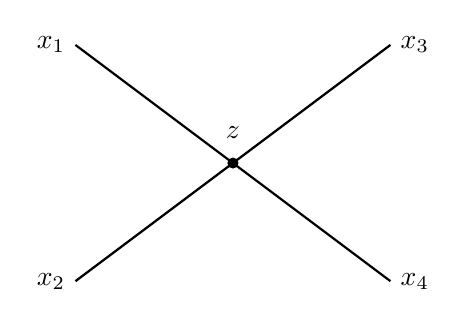
\begin{tikzpicture}[line width=.8pt,line label/.style={fill=white,fill opacity=.96,text opacity=1,inner sep=1.15pt}]
  \coordinate (v) at (0,0);
  \draw (v)--(-2,1.5) node[left]{$x_1$};
  \draw (v)--(-2,-1.5) node[left]{$x_2$};
  \draw (v)--(2,1.5) node[right]{$x_3$};
  \draw (v)--(2,-1.5) node[right]{$x_4$};
  \fill (v) circle (2pt) node[above=5pt]{$z$};
 \end{tikzpicture}
 \caption{$\varphi^4$ 理论四点 Green 函数的最低阶连通图。图只是\eqnrefs{eq:phi4-tree-green-r3} 中四个传播子与一次相互作用插入的图形缩写。}
 \label{fig:phi4-first-diagram-r3}
\end{figure}

同一 Dyson 展开在有限作用时间下还给出 Fermi 黄金律的来源。对时间无关微扰 $V$ 在时间窗 $T$ 内的一阶跃迁，定义能量失谐 $\Delta E\equiv E_f-E_i$，则有限时间概率核为
\begin{equation}
 \boxed{
 |c_f^{(1)}(T)|^2
 =\frac{|V_{fi}|^2T^2}{\hbar^2}
 \operatorname{sinc}^2\!\left(\frac{\Delta E\,T}{2\hbar}\right).}
 \label{eq:golden-sinc-r3}
\end{equation}
只有对平滑连续态密度 $\nu_f(E)$ 积分并取长时间极限，才可使用 $\sinc^2\to\delta$ 的分布极限，得到
\begin{equation}
 \boxed{
 w_{i\to f}
 =\frac{2\pi}{\hbar}|V_{fi}|^2\nu_f(E_i).}
 \label{eq:fermi-golden-r3}
\end{equation}
因此有限时间振幅先产生宽度约为 $1/T$ 的 sinc 谱核；在对平滑末态谱求和并取 $T\to\infty$ 后，该核才以分布极限收缩为能量守恒 $\delta$ 函数。

前面的自由场配对定理和图规则仍然使用自由场的产生、湮灭算符，但真实散射实验中的“入射电子”和“出射电子”属于相互作用理论。要把相关函数连接到实验散射振幅，必须先说明相互作用理论为什么在遥远过去和未来仍能定义自由的入射、出射粒子。

设相互作用理论存在稳定的单粒子态，物理质量为 $m_{\rm phys}$。把完整 Heisenberg 场记为 $\varphi_H(x)$。在遥远过去和遥远未来，彼此分离的稳定粒子已经离开有限的散射区，因此可分别引入自由的入场和出场
\begin{equation}
 \left(\Box+\frac{m_{\rm phys}^2c^2}{\hbar^2}\right)
 \varphi_{\rm in/out}(x)=0.
 \label{eq:asymptotic-free-field-dp48}
\end{equation}
它们各自具有与自由场相同形式的模展开，只是产生、湮灭算符分别记为 $a_{\rm in/out}(\mathbf p)$。于是
\begin{equation*}
 |\mathbf p;{\rm in}\rangle
 =a_{\rm in}^\dagger(\mathbf p)|\Omega\rangle,
 \qquad
 |\mathbf p;{\rm out}\rangle
 =a_{\rm out}^\dagger(\mathbf p)|\Omega\rangle,
\end{equation*}
其中 $|\Omega\rangle$ 是相互作用理论的真空。多粒子入态、出态由相应产生算符继续构造，而实验散射振幅的起点正是
\begin{equation}
 \boxed{S_{fi}=\langle f,{\rm out}|i,{\rm in}\rangle.}
 \label{eq:in-out-smatrix-dp48}
\end{equation}
这一定义把“远处可以识别的粒子”与“相互作用区内复杂的量子场”明确分开。


对无导数标量相互作用，$\pi_H=c^{-2}\partial_t\varphi_H$。自由场模展开~\eqnrefs{eq:scalar-mode-r2} 可以逐模反演，因此对完整 Heisenberg 场定义有限时刻的单粒子投影算符
\begin{equation}
 \hat a_t(\mathbf p)
 \equiv\int\dd^3 x\,\ee^{+\ii p\cdot x/\hbar}
 \left[
 \frac{1}{\hbar c}\sqrt{\frac{E_{\mathbf p}}{2}}\,\varphi_H(x)
 +\frac{\ii c}{\sqrt{2E_{\mathbf p}}}\,\pi_H(x)
 \right],
 \label{eq:lsz-finite-time-mode-projection-dp52}
\end{equation}
其中指数中的 $p^0=E_{\mathbf p}/c$ 取物理质量壳值。若 $\varphi_H$ 本身就是自由场，\eqnrefs{eq:lsz-finite-time-mode-projection-dp52} 精确返回 $\hat a(\mathbf p)$；存在相互作用时，它会随 $t$ 改变，因为局域场在散射区内不断与多粒子扇区混合。

稳定单粒子极点意味着在足够早和足够晚的时刻，完整场在单粒子方向上的投影趋于自由入、出模。用极点留数 $Z$ 修正局域场与归一化粒子态之间的重叠，定义
\begin{equation}
 \boxed{
 \hat a_{\rm in/out}(\mathbf p)
 =Z^{-1/2}\lim_{t\to\mp\infty}\hat a_t(\mathbf p).}
 \label{eq:asymptotic-annihilator-projection-dp52}
\end{equation}
对\eqnrefs{eq:lsz-finite-time-mode-projection-dp52} 求时间导数，再把空间 Laplace 项分部积分到平面波上，可得
\begin{equation}
 \boxed{
 \hat a_{\rm out}(\mathbf p)-\hat a_{\rm in}(\mathbf p)
 =\frac{\ii Z^{-1/2}}{\sqrt{2E_{\mathbf p}}}
 \int\dd^4 x\,
 \ee^{+\ii p\cdot x/\hbar}
 \left(\Box+\frac{m_{\rm phys}^2c^2}{\hbar^2}\right)
 \varphi_H(x).}
 \label{eq:lsz-one-leg-position-dp52}
\end{equation}
这里 $x^0=ct$，所以 $\dd^4 x=c\,\dd t\,\dd^3 x$。\eqnrefs{eq:lsz-one-leg-position-dp52} 已经建立了外腿约化的核心桥梁：每把一个标量渐近粒子从外态移入时序关联函数，就会在相应外部坐标上作用一次自由标量逆核 $\Box+m_{\rm phys}^2c^2/\hbar^2$。电子外腿不能沿用这一二阶算符；对自旋 $1/2$ 电子，截肢由一阶 Dirac 逆算符 $\ii\hbar\slashed\partial-\me c$ 完成。第 4 章将从 Dirac 二点函数本身建立其极点分子与外腿结构。对所有外腿分别作用与其 Lorentz 表示相匹配的自由逆算符，再 Fourier 变换，才得到相应的动量空间截肢公式。这整套由单粒子极点把时序相关函数转换成渐近散射振幅的步骤称为\emph{Lehmann--Symanzik--Zimmermann 约化}，简称 LSZ 约化。

完整场并不等于入场或出场。稳定单粒子态在精确二点函数中表现为与连续谱分支切割分离的孤立极点：
\begin{equation}
 \boxed{
 \widetilde G_2(p)
 =\frac{\ii\hbar^3c\,Z}{p^2-m_{\rm phys}^2c^2+\ii0^+}
 +\widetilde G_{2,\rm cont}(p).}
 \label{eq:lsz-pole-plus-cont-r7}
\end{equation}
$Z$ 是所选局域场与物理单粒子态的无量纲交叠留数；等价地说，$Z^{1/2}$ 衡量 $\varphi_H$ 在稳定单粒子极点附近与相应渐近自由场的重叠。因此 LSZ 中出现的 $Z^{-1/2}$ 不是人为补上的归一化常数，而是把“局域场插入”换成“归一化渐近粒子”的必要因子。

LSZ 外腿要求与连续谱分开的稳定单粒子极点。具有有限寿命的共振对应复能量平面上的极点，不能作为 $t\to\pm\infty$ 的自由渐近粒子；它只能通过内部共振传播或连续谱进入散射振幅。

对连通 $n$ 点函数，最清楚的写法不是用一个模糊的“近似于”符号，而是在每个外部质量壳附近作多变量 Laurent 分解。定义
\[
 \zeta_i\equiv p_i^2-m_i^2c^2,
\]
并先把 $\zeta_i$ 视为复变量；Feynman 的 $+\ii0^+$ 只规定最后从哪一侧取实轴边界值。则在稳定单粒子极点的邻域内可以写成精确分解
\begin{equation}
 \boxed{
 \widetilde G_{n,c}
 =
 (2\pi\hbar)^4\delta^{(4)}\!\left(\sum_i\sigma_i^{\rm io}p_i\right)
 \left[\prod_i
 \frac{\ii\hbar^3c\,Z_i^{1/2}}
 {\zeta_i+\ii0^+}\right]
 \ii\mathfrak A_{fi}(\{p_i\})
 +\widetilde R_n(\{p_i\}),}
 \label{eq:LSZ-factorization-r7}
\end{equation}
其中入射/出射外线分别取 $\sigma_i^{\rm io}=+1,-1$；$\mathfrak A_{fi}(\{p_i\})$ 在所有 $\zeta_i=0$ 的联合邻域内正则，而余项 $\widetilde R_n$ 的定义性质是它至少缺少一条外部单粒子极点，因此
\[
 \lim_{\zeta_1,\ldots,\zeta_n\to0}
 \left(\prod_i\zeta_i\right)\widetilde R_n=0.
\]
这一定义把“外腿极点”和“真正的相互作用核”严格分开。于是 LSZ 约化的核心就是先用逆极点因子截去外线传播子，再取在壳极限：
\begin{equation}
 \boxed{
 \lim_{p_i^2\to m_i^2c^2}
 \left[\prod_i
 Z_i^{-1/2}\frac{p_i^2-m_i^2c^2}{\ii\hbar^3c}\right]
 \widetilde G_{n,c}
 =(2\pi\hbar)^4\delta^{(4)}(P_f-P_i)\,\ii\mathfrak A_{fi}.}
 \label{eq:lsz-momentum-reduction-r7}
\end{equation}
对上面的 $\varphi^4$ 树图，四条外线传播子全部被这一操作消去，只留下
\begin{equation}
 \boxed{
 (2\pi\hbar)^4\delta^{(4)}(p_1+p_2-p_3-p_4)
 \left(-\frac{\ii g_4}{\hbar^2c^2}\right).}
 \label{eq:phi4-lsz-result-r7}
\end{equation}
因此外线传播子的截除来自精确单粒子极点的因子化。旋量与光子外线分别由相应的矩阵值逆动能算符完成截肢。

Dyson 级数产生自由场的时序乘积，Wick 定理把它们化为传播子与顶角，有限时间谱核说明能量守恒如何从长时间极限进入跃迁率，而精确单粒子极点再经 LSZ 约化把 Green 函数连接到渐近 $S$ 矩阵元。这四层共同构成微扰散射的算符基础。


% -----------------------------------------------------------------------------
% -----------------------------------------------------------------------------

\begin{exbox}[四点 Green 函数到截面]
前面的 LSZ 公式如果只停留在“给每条外腿乘一个逆传播子”，初学者很容易把它记成形式操作。最简单的检查是把 $\varphi^4$ 树级四点函数从头带一遍。相互作用仍取
\begin{equation*}
 \Lag_{\rm int}=-\frac{g_4}{4!\,\hbar c}\varphi^4,
 \qquad [g_4]=1,
\end{equation*}
而物理四动量满足 $p_i^2=m^2c^2$。在动量空间中，四点连通函数的最低阶奇异部分可以写成
\begin{equation}
 \begin{aligned}
 \widetilde G_{4,c}^{(1)}
 =&\,(2\pi\hbar)^4\delta^{(4)}(p_1+p_2-p_3-p_4)
 \left(-\frac{\ii g_4}{\hbar^2c^2}\right)\\
 &\times\prod_{a=1}^{4}
 \frac{\ii\hbar^3c}{p_a^2-m^2c^2+\ii0^+}.
 \end{aligned}
 \label{eq:phi4-fourpoint-poles-dp64}
\end{equation}
这个式子里其实混着三种不同信息：四维 $\delta$ 函数来自顶角位置积分；中间常数来自局域四价顶角；四个简单极点只是“从相互作用点传播到四个外部场插入点”的外腿传播。实验制备的是渐近单粒子，而不是带着这四个外腿传播子的场插入，因此 LSZ 要做的正是把最后一层剥掉。

对四条外腿逐一乘
\begin{equation*}
 \frac{p_a^2-m^2c^2}{\ii\hbar^3c}
\end{equation*}
并取 $p_a^2\to m^2c^2$，四个极点逐个相消，只留下
\begin{equation*}
 (2\pi\hbar)^4\delta^{(4)}(P_f-P_i)
 \left(-\frac{\ii g_4}{\hbar^2c^2}\right).
\end{equation*}
按上述约化振幅的统一定义，把纯粹来自 SI 场归一化的公共因子 $1/(\hbar^2c^2)$ 提出后，真正进入散射母式的是无量纲结果
\begin{equation}
 \boxed{\mathcal M_{\varphi\varphi\to\varphi\varphi}=-g_4.}
 \label{eq:phi4-reduced-amplitude-dp64}
\end{equation}
因此“图上四条外腿”与“物理振幅里的四个外粒子”不是同一件东西：前者在 Green 函数里带单粒子极点，后者经过 LSZ 后只保留在壳外态标签。

\eqnrefs{eq:phi4-reduced-amplitude-dp64} 代入二体截面母式后，等质量弹性散射有 $|\mathbf p_f|=|\mathbf p_i|$；末态两个标量完全相同，所以有额外的 $1/2!$。于是
\begin{equation*}
 \frac{\dd\sigma}{\dd\Omega}
 =\frac12\frac{\hbar^2}{64\pi^2s}g_4^2
 =\frac{\hbar^2g_4^2}{128\pi^2s},
\end{equation*}
这就是接触四点相互作用的各向同性二体截面。由于接触顶角没有任何 $t$ 或 $u$ 依赖，角分布各向同性；积分整个立体角后
\begin{equation}
 \boxed{
 \sigma_{\rm tot}
 =\frac{\hbar^2g_4^2}{32\pi s}.}
 \label{eq:phi4-total-cross-dp64}
\end{equation}
若用质心能量 $E_{\rm CM}=c\sqrt{s}$ 表示，便有
\begin{equation*}
 \sigma_{\rm tot}
 =\frac{g_4^2}{32\pi}
 \left(\frac{\hbar c}{E_{\rm CM}}\right)^2.
\end{equation*}
这最后一行也提供了一个快速量纲检查：四维无导数接触相互作用的无量纲耦合不提供长度尺度，因此高能截面只能按 $E_{\rm CM}^{-2}$ 衰减。作为数量级练习，若取 $g_4=0.50$、$E_{\rm CM}=1.00\,\mathrm{GeV}$，用 $\hbar c=0.19732698\,\mathrm{GeV\,fm}$ 得
\begin{align*}
 \sigma_{\rm tot}
 &=\frac{0.50^2}{32\pi}
 \left(\frac{0.19732698\,\mathrm{GeV\,fm}}{1.00\,\mathrm{GeV}}\right)^2,\\
 &\simeq9.68\times10^{-5}\,\mathrm{fm^2}
 =9.68\times10^{-35}\,\mathrm{m^2}
 \simeq0.968\,\mu\mathrm b.
\end{align*}
这个数值没有新的物理输入，只是在训练从自然出现的 $\hbar c/E$ 长度尺度回到实验常用的截面单位。


\medskip

\eqnrefs{eq:phi4-fourpoint-poles-dp64} 已把最低阶四点函数分成总四动量守恒、局域四价顶角和四条单粒子外腿极点。LSZ 约化作用在四条单粒子外腿极点上；直接检查四个在壳极点怎样逐个与约化算符相消。这里保留树级 $Z=1$，外部标量均视为稳定单粒子态。

对第 $a$ 条外腿定义逆极点因子
\[
 R_a(p_a)
 \equiv
 \frac{p_a^2-m^2c^2}{\ii\hbar^3c}.
\]
由\eqnrefs{eq:phi4-fourpoint-poles-dp64} 中的单腿因子可得
\[
 \lim_{p_a^2\to m^2c^2}
 R_a(p_a)
 \frac{\ii\hbar^3c}{p_a^2-m^2c^2+\ii0^+}=1.
\]
四条外腿分别取同一极限后，传播子极点全部消失，而顶角与总四动量守恒保留：
\[
 \lim_{p_a^2\to m^2c^2}
 \prod_{a=1}^{4}R_a(p_a)\,
 \widetilde G_{4,c}^{(1)}
 =(2\pi\hbar)^4\delta^{(4)}(P_f-P_i)
 \left(-\frac{\ii g_4}{\hbar^2c^2}\right).
\]
按前文约化振幅的 SI 归一化约定，把公共场归一化因子 $1/(\hbar^2c^2)$ 提出，得到
\[
 \ii\mathcal M=-\ii g_4,
 \qquad
 \mathcal M_{\varphi\varphi\to\varphi\varphi}=-g_4,
\]
即\eqnrefs{eq:phi4-reduced-amplitude-dp64}。


\medskip

\eqnrefs{eq:phi4-reduced-amplitude-dp64} 已经是可直接送入散射相空间的无量纲在壳振幅。剩下只需处理二体通量、全同末态计数和立体角积分；这一阶段不再涉及 LSZ 或 Green 函数。等质量弹性散射满足 $|\mathbf p_f|=|\mathbf p_i|$，而两个末态是同种实标量，因此二体截面母式中的对称因子为 $1/2!$。

由\eqnrefs{eq:2to2-cross-section-master-si-r9}，
\[
 \frac{\dd\sigma}{\dd\Omega}
 =\frac1{2!}\frac{\hbar^2}{64\pi^2s}
 |\mathcal M|^2
 =\frac{\hbar^2g_4^2}{128\pi^2s}.
\]
接触振幅没有 $t$ 或 $u$ 依赖，因此角分布各向同性。积分 $\int\dd\Omega=4\pi$ 得
\[
 \sigma_{\rm tot}
 =4\pi\frac{\hbar^2g_4^2}{128\pi^2s}
 =\frac{\hbar^2g_4^2}{32\pi s},
\]
即\eqnrefs{eq:phi4-total-cross-dp64}。
\end{exbox}





\begin{derivation}[从\eqnrefs{eq:wick-generating-identity-dp74}到\eqnrefs{eq:wick-general-r3}]
把生成恒等式写成“正规序线性源”与“收缩二次源”的乘积：
\begin{equation*}
 \mathcal T\exp\!\left[
 \frac{\ii}{\hbar c}\int\dd^4x\,\mathcal J(x)\varphi(x)
 \right]
 =:\exp\!\left[
 \frac{\ii}{\hbar c}\int\dd^4x\,\mathcal J(x)\varphi(x)
 \right]:
 \exp\!\left[-\frac{1}{2\hbar^2c^2}
 \int\dd^4x\dd^4y\,\mathcal J(x)\Delta_F(x-y)\mathcal J(y)
 \right].
\end{equation*}
要得到 $n$ 个指定场 $\varphi_r\equiv\varphi(x_r)$ 的时间序乘积，对两边作 $n$ 次源泛函微分后令 $\mathcal J=0$。非零项中，每一个微分只有两种去处：命中正规序指数的一次源，留下一个未收缩场；或者与另一个微分共同命中二次源指数中的同一个 $\mathcal J(x)\mathcal J(y)$，产生一条二点收缩 $\Delta_F(x_r-x_s)$。

固定恰有 $k$ 条收缩。需要从 $n$ 个标签中选择 $2k$ 个参与收缩，再把它们配成 $k$ 对。带标签配对数为
\begin{equation*}
 \binom{n}{2k}\frac{(2k)!}{2^k k!}
 =\frac{n!}{(n-2k)!2^k k!}.
\end{equation*}
这个组合因子可以直接从二次指数的展开系数看出。其第 $k$ 阶是
\begin{equation*}
 \frac{1}{k!}
 \left[-\frac{1}{2\hbar^2c^2}
 \int\dd^4x\dd^4y\,
 \mathcal J(x)\Delta_F(x-y)\mathcal J(y)
 \right]^k.
\end{equation*}
$n$ 次微分中命中这 $2k$ 个源的排列产生 $(2k)!$；每条二次因子内部交换两个端点产生 $2^k$ 重数，而 $k$ 条二次因子之间交换又产生 $k!$ 重数。原系数中的 $1/(2^kk!)$ 恰好把这些“同一无序配对的重复计数”除掉，所以每一个具体部分配对只留下系数 1。

因此若 $P$ 表示标签集合 $\{1,\ldots,n\}$ 的任意部分配对，$V(P)$ 表示所有已参与配对的标签，则
\begin{equation*}
 \mathcal T\!\left\{\prod_{r=1}^n\varphi_r\right\}
 =\sum_{P}
 \left[\prod_{(r,s)\in P}\Delta_F(x_r-x_s)\right]
 :\!\prod_{j\notin V(P)}\varphi_j\!:,
\end{equation*}
即正文\eqnrefs{eq:wick-general-r3}。

例如 $n=4$ 时，$k=2$ 的完全收缩数为
$4!/(2^2 2!)=3$，正是
$\Delta_{12}\Delta_{34}$、$\Delta_{13}\Delta_{24}$、$\Delta_{14}\Delta_{23}$ 三项。这个低阶检查同时说明 Wick 定理的组合系数来自源导数，而不是费曼图规则额外规定的权重。
\end{derivation}

\begin{derivation}[从\eqnrefs{eq:phi4-first-dyson-r68}到\eqnrefs{eq:phi4-tree-green-r3}]

正文\eqnrefs{eq:phi4-first-dyson-r68} 是 $\varphi^4$ 理论四点函数的一阶 Dyson 插入。连通树级项要求每个外场都与顶点 $z$ 上四个场中的一个且仅一个收缩，因此共有 $4!$ 种相同配对；它们与作用量中的 $1/4!$ 抵消后得到正文\eqnrefs{eq:phi4-tree-green-r3}。



四点函数的一阶 Dyson 项为
\begin{equation*}
 G^{(4,1)}(x_1,x_2,x_3,x_4)
 =-\frac{\ii g_4}{4!\,\hbar^2c^2}
 \int\dd^4 z\,
 \langle0|\Tord\{\varphi_1\varphi_2\varphi_3\varphi_4\varphi^4(z)\}|0\rangle .
\end{equation*}
要得到“一个顶点连接四个外点”的连通树图，每个外部场必须与 $z$ 点四个场中的一个且仅一个收缩。先给 $\varphi_1$ 选 $z$ 点场有 $4$ 种；再给 $\varphi_2$ 选剩余场有 $3$ 种；之后分别有 $2$ 种和 $1$ 种，所以
\begin{equation*}
 N_{\rm contr}=4\times3\times2\times1=4!.
\end{equation*}
每一种收缩都给出同一个核乘积
\begin{equation*}
 \Delta_F(x_1-z)\Delta_F(x_2-z)\Delta_F(x_3-z)\Delta_F(x_4-z).
\end{equation*}
因此 $4!$ 个相同项与相互作用中的 $1/4!$ 抵消，得到
\begin{equation*}
 G_c^{(4)}
 =-\frac{\ii g_4}{\hbar^2c^2}
 \int\dd^4 z\,\prod_{a=1}^4\Delta_F(x_a-z),
\end{equation*}
即正文\eqnrefs{eq:phi4-tree-green-r3}。

再把四条外线分别 Fourier 展开。四个传播子的指数中所有 $z$ 依赖合成
\begin{equation*}
 \exp\!\left[-\frac{\ii}{\hbar}
 (p_1+p_2-p_3-p_4)\cdot z\right].
\end{equation*}
于是顶角位置积分给
\begin{equation*}
 \int\dd^4 z\,
 \ee^{-\ii(p_1+p_2-p_3-p_4)\cdot z/\hbar}
 =(2\pi\hbar)^4\delta^{(4)}(p_1+p_2-p_3-p_4).
\end{equation*}
所以顶角四动量守恒正是局域相互作用对顶角位置积分后的 Fourier $\delta$ 函数。
\end{derivation}

\begin{derivation}[从\eqnrefs{eq:golden-sinc-r3}到\eqnrefs{eq:fermi-golden-r3}]
记 $\Delta E=E_f-E_i$。一阶振幅为

\begin{align*}
 c_f^{(1)}(T)
 &=-\frac{\ii}{\hbar}V_{fi}
 \int_{-T/2}^{T/2}\dd t\,\ee^{\ii\Delta E t/\hbar}\\
 &=-\frac{\ii}{\hbar}V_{fi}
 \left[\frac{\hbar}{\ii\Delta E}
 \ee^{\ii\Delta E t/\hbar}\right]_{-T/2}^{T/2}\\
 &=-\frac{2\ii V_{fi}}{\Delta E}
 \sin\!\left(\frac{\Delta E T}{2\hbar}\right).
\end{align*}
把 $\sinc x\equiv\sin x/x$ 提出，得到
\begin{equation*}
 |c_f^{(1)}(T)|^2
 =\frac{|V_{fi}|^2T^2}{\hbar^2}
 \sinc^2\!\left(\frac{\Delta E T}{2\hbar}\right),
\end{equation*}
即\eqnrefs{eq:golden-sinc-r3}。它在有限 $T$ 时不是 $\delta$ 函数；主峰宽度量级是 $\hbar/T$。

对连续末态求和，概率为
\begin{equation*}
 P_{i\to f}(T)
 =\int\dd E\,\nu_f(E)
 \frac{|V_{fi}(E)|^2T^2}{\hbar^2}
 \sinc^2\!\left[\frac{(E-E_i)T}{2\hbar}\right].
\end{equation*}
这里 $\nu_f(E)$ 是末态每单位能量的态密度，SI 量纲为 $\mathrm{J^{-1}}$。有限时间谱核与 Dirac $\delta$ 分布的对应由下列核固定：
\begin{equation*}
 K_T(\Delta E)
 \equiv
 \frac{T}{2\pi\hbar}
 \sinc^2\!\left(\frac{\Delta E\,T}{2\hbar}\right).
\end{equation*}
它具有能量倒数量纲。作变量代换 $x=\Delta E T/(2\hbar)$ 后，
\begin{align*}
 \int_{-\infty}^{+\infty}\dd(\Delta E)\,K_T(\Delta E)
 &=\frac{T}{2\pi\hbar}
 \frac{2\hbar}{T}
 \int_{-\infty}^{+\infty}\dd x\,\sinc^2x\\
 &=\frac1\pi\int_{-\infty}^{+\infty}\dd x\,\sinc^2x=1.
\end{align*}
因此 $K_T$ 是面积固定为一、宽度随 $T^{-1}$ 收缩的归一化谱核；对任意在 $E_i$ 附近平滑的测试函数 $F(E)$，$T\to\infty$ 时满足
\begin{equation*}
 \int\dd E\,F(E)K_T(E-E_i)\longrightarrow F(E_i),
\end{equation*}
也就是 $K_T(\Delta E)\to\delta(\Delta E)$ 的分布极限。
令
\begin{equation*}
F(E)\equiv |V_{fi}(E)|^2\nu_f(E).
\end{equation*}
由 $K_T$ 的定义，有限时间概率可以严格改写为
\begin{equation*}
P_{i\to f}(T)
=\frac{2\pi T}{\hbar}
\int\dd E\,F(E)K_T(E-E_i).
\end{equation*}
再定义有限时间余项
\begin{equation*}
\delta F_T
\equiv
\int\dd E\,[F(E)-F(E_i)]K_T(E-E_i),
\end{equation*}
利用 $\int K_T\dd E=1$ 得到精确等式
\begin{equation*}
P_{i\to f}(T)
=\frac{2\pi T}{\hbar}[F(E_i)+\delta F_T].
\end{equation*}
前面已经证明 $K_T\to\delta$ 的分布极限，所以对满足该近似恒等核收敛条件的连续 $F$，有 $\lim_{T\to\infty}\delta F_T=0$。因此长时间跃迁率严格由极限定义
\begin{equation*}
\lim_{T\to\infty}\frac{P_{i\to f}(T)}{T}
=\frac{2\pi}{\hbar}F(E_i).
\end{equation*}
也就是
\begin{equation*}
 w_{i\to f}=\frac{2\pi}{\hbar}|V_{fi}|^2\nu_f(E_i),
\end{equation*}
即 Fermi 黄金律~\eqnrefs{eq:fermi-golden-r3}。能量 $\delta$ 分布由有限时间谱核与连续谱卷积的长时间极限产生；有限 $T$ 时应保留具有有限宽度的 $\sinc^2$ 核。
\end{derivation}

% Detailed derivations gathered at the end of the owning structure.

\begin{derivation}[从\eqnrefs{eq:generic-fermion-contraction-dp8}到\eqnrefs{eq:fermion-wick-four-r68}]

正文\eqnrefs{eq:generic-fermion-contraction-dp8} 定义了自由费米场的一次收缩。对两对费米场只有直接配对和交叉配对两种完全收缩，而后者相对前者多一次 Grassmann 奇置换；把两项相加便得到正文\eqnrefs{eq:fermion-wick-four-r68}。



考虑固定初始顺序
\begin{equation*}
 \mathscr W_4
 =\langle0|T\{\psi_1\bar\psi_2\psi_3\bar\psi_4\}|0\rangle.
\end{equation*}
自由真空期望值必须把每个 $\psi$ 与一个 $\bar\psi$ 配对。第一种配对是 $(1,2)(3,4)$；两对在原顺序中已经相邻，因此不需要额外奇置换，贡献
\begin{equation*}
 +S_{12}S_{34}.
\end{equation*}
第二种配对是 $(1,4)(3,2)$。$\bar\psi_4$ 与 $\psi_1$ 收缩时必须越过中间的费米算符；等价地说，从配对 $(1,2)(3,4)$ 变到交叉配对改变了一次配对排列的宇称，因此贡献带负号。于是
\begin{equation*}
 {
 \mathscr W_4=S_{12}S_{34}-S_{14}S_{32}.}
 \end{equation*}
这个负号不是某个 QED 顶角的性质；即使没有电磁相互作用，自由费米高斯也已经具有它。

一般地，考虑 $n$ 个 $\psi_i$ 与 $n$ 个 $\bar\psi_j$。每个完全收缩等价于一个置换 $\pi\in S_n$，把第 $i$ 个 $\psi_i$ 配到 $\bar\psi_{\pi(i)}$。每次交换 Grassmann-odd 算符都产生 $-1$，故
\begin{equation*}
 \langle0|T\{\psi_1\bar\psi_1\cdots\psi_n\bar\psi_n\}|0\rangle
 =\sum_{\pi\in S_n}
 \operatorname{sgn}(\pi)
 \prod_{i=1}^{n}S_{i,\pi(i)}.
 \end{equation*}
右边正是矩阵 $S_{ij}$ 的行列式：
\begin{equation*}
 {
 \langle T\,\psi_1\bar\psi_1\cdots\psi_n\bar\psi_n\rangle_0
 =\det[S_{ij}].}
 \end{equation*}
与此相对，玻色高斯的完全收缩是不含 $\operatorname{sgn}(\pi)$ 的积和式配对和。Grassmann 高斯积分产生行列式，普通高斯积分产生行列式的负幂；它们与这里的 Wick 组合计数是同一反对易结构的不同表现。
\end{derivation}

\begin{derivation}[从\eqnrefs{eq:generic-fermion-contraction-dp8}到\eqnrefs{eq:generic-closed-fermion-loop-r68}]
在相互作用展开中，若若干费米收缩连成闭环，例如取如下示意性的双线性乘积

\begin{equation*}
 (\bar\psi_1\Gamma_1\psi_1)
 (\bar\psi_2\Gamma_2\psi_2)\cdots
 (\bar\psi_n\Gamma_n\psi_n),
\end{equation*}
并取循环收缩
\begin{equation*}
 \psi_1\leftrightarrow\bar\psi_2,
 \quad
 \psi_2\leftrightarrow\bar\psi_3,
 \quad\ldots\quad
 \psi_n\leftrightarrow\bar\psi_1,
\end{equation*}
则配对置换是一个长度为 $n$ 的循环。长度为 $n$ 的循环可分解成 $n-1$ 次对换，所以其宇称为 $(-1)^{n-1}$。另一方面，把每个双线性型中的 $\bar\psi_i$ 移到用于写矩阵迹的统一位置还产生 $(-1)^n$。两者相乘为
\begin{equation*}
 (-1)^{n-1}(-1)^n=-1.
\end{equation*}
因此一个闭合费米子圈相对于同样连接结构的对易的场多出
\begin{equation*}
 {-1.}
 \end{equation*}
下一章 QED 真空极化的迹
$-\operatorname{Tr}[\gamma^\mu S_F\gamma^\nu S_F]$
就是这个一般结论的具体实例。
\end{derivation}

\begin{derivation}[从\eqnrefs{eq:lsz-pole-plus-cont-r7}到\eqnrefs{eq:phi4-lsz-result-r7}]
先只处理一条外腿，因为多腿公式只是把同一个极点提取操作重复 $n$ 次。设 $\zeta=p^2-m_{\rm phys}^2c^2$，并把 $\zeta$ 暂时视为复变量。对时序关联函数中与坐标 $x$ 对应的那一个场插入完整态，稳定单粒子态给出
\begin{equation*}
 \langle\Omega|\varphi_H(0)|p,\lambda\rangle
 =Z^{1/2}\,\mathcal N_p,
\end{equation*}
其中 $\mathcal N_p$ 是由全书协变态归一化固定的运动学因子。把该单粒子贡献与其余所有中间态分开，Fourier 变换后必然具有形式
\begin{equation*}
 \widetilde G_{n,c}(p,\ldots)
 =\frac{\ii\hbar^3c\,Z^{1/2}}
 {\zeta}\,
 \widetilde F_{n-1}(p;\ldots)
 +\widetilde R^{(1)}_n(p,\ldots),
\end{equation*}
这里 $\widetilde F_{n-1}$ 是已经把这一条外腿换成归一化单粒子态后的矩阵元；$\widetilde R^{(1)}_n$ 包含连续谱和在这一外部通道中正则的项。稳定粒子极点与多粒子阈值分离，所以在 $\zeta=0$ 的一个小邻域内
\begin{equation*}
 \lim_{\zeta\to0}\zeta\,\widetilde R^{(1)}_n=0.
\end{equation*}
因此极点留数不是一句“外腿传播子可以删掉”，而是如下复分析极限：
\begin{align*}
 \lim_{\zeta\to0}
 Z^{-1/2}\frac{\zeta}{\ii\hbar^3c}
 \widetilde G_{n,c}
 &=\lim_{\zeta\to0}
 \left[
 \widetilde F_{n-1}
 +Z^{-1/2}\frac{\zeta}{\ii\hbar^3c}
 \widetilde R^{(1)}_n
 \right]\\
 &=\widetilde F_{n-1}(p_{\rm on};\ldots).
\end{align*}
Feynman 的 $+\ii0^+$ 是实动量边界值的处方；截肢本身应理解为先在复 $\zeta$ 平面取极点留数，再回到质量壳，因此不会出现把 $\zeta/(\zeta+\ii0^+)$ 当作普通数值比值的歧义。

对第二、第三直到第 $n$ 条外腿重复同一操作。若定义 $\zeta_i=p_i^2-m_i^2c^2$，则联合极点邻域中的多变量 Laurent 展开可写成
\begin{align*}
 \widetilde G_{n,c}
 ={}&(2\pi\hbar)^4\delta^{(4)}\!\left(\sum_i\sigma_i^{\rm io}p_i\right)
 \left[\prod_i
 \frac{\ii\hbar^3c\,Z_i^{1/2}}{\zeta_i}\right]
 \ii\mathfrak A_{fi}(\{p_i\})
 +\widetilde R_n,\\
 &\lim_{\zeta_1,\ldots,\zeta_n\to0}
 \left(\prod_i\zeta_i\right)\widetilde R_n=0.
\end{align*}
第二行正是“余项至少缺少一条完整外腿极点”的数学含义。于是
\begin{align*}
 &\lim_{\zeta_1,\ldots,\zeta_n\to0}
 \left[\prod_iZ_i^{-1/2}
 \frac{\zeta_i}{\ii\hbar^3c}\right]
 \widetilde G_{n,c}\\
 &\qquad=(2\pi\hbar)^4\delta^{(4)}\!\left(\sum_i\sigma_i^{\rm io}p_i\right)
 \ii\mathfrak A_{fi}(\{p_{i,\rm on}\}),
\end{align*}
这就得到正文的动量空间 LSZ 公式。注意截肢和在壳极限的顺序来自极点留数的定义：先乘 $\zeta_i$ 提取留数，再令 $\zeta_i\to0$；若反过来，原 Green 函数正好落在极点上。

现在把这一抽象结构用于树级 $\varphi^4$。一次 Dyson 插入给
\begin{equation*}
 -\frac{\ii}{\hbar c}
 \int\dd^4x\,
 \frac{g_4}{4!\,\hbar c}\,
 \varphi_I(x)^4.
\end{equation*}
把四个外部场分别与顶角处四个场收缩有 $4!$ 种双射，恰好消掉相互作用中的 $1/4!$。每条收缩给一个自由 Feynman 传播子，所以 Fourier 变换后的连通四点函数为
\begin{equation*}
 \widetilde G^{(1)}_{4,c}
 =-\frac{\ii g_4}{\hbar^2c^2}
 (2\pi\hbar)^4\delta^{(4)}(p_1+p_2-p_3-p_4)
 \prod_{a=1}^{4}
 \frac{\ii\hbar^3c}{p_a^2-m^2c^2+\ii0^+}.
\end{equation*}
在树级 $Z=1$。令 $\zeta_a=p_a^2-m^2c^2$，逐腿乘逆极点因子后，乘积中的四条外腿逐一消去：
\begin{align*}
 &\left[\prod_{a=1}^{4}
 \frac{\zeta_a}{\ii\hbar^3c}\right]
 \widetilde G^{(1)}_{4,c}\\
 &\quad=-\frac{\ii g_4}{\hbar^2c^2}
 (2\pi\hbar)^4\delta^{(4)}(p_1+p_2-p_3-p_4)
 \prod_{a=1}^{4}
 \frac{\zeta_a}{\zeta_a+\ii0^+}.
\end{align*}
按上面说明的极点留数顺序取极限，四个因子都贡献单位留数，于是得到正文\eqnrefs{eq:phi4-lsz-result-r7}。因此树级顶角规则不是另记的一条口诀：$4!$ 来自 Wick 收缩计数，四条传播子来自外部收缩，而 LSZ 的四个逆极点恰好把这些外腿传播子截去，只留下局域顶角系数。
\end{derivation}


\begin{derivation}[从\eqnrefs{eq:lsz-finite-time-mode-projection-dp52}到\eqnrefs{eq:lsz-one-leg-position-dp52}]
先验证有限时刻投影式的归一化。把自由场展开~\eqnrefs{eq:scalar-mode-r2} 与

\begin{equation*}
 \pi(x)=\frac{1}{c^2}\partial_t\varphi(x)
 =-\ii\int\frac{\dd^3 q}{(2\pi\hbar)^3}
 \sqrt{\frac{E_{\mathbf q}}{2c^2}}
 \left[
 a(\mathbf q)\ee^{-\ii q\cdot x/\hbar}
 -a^\dagger(\mathbf q)\ee^{+\ii q\cdot x/\hbar}
 \right]
\end{equation*}
代入\eqnrefs{eq:lsz-finite-time-mode-projection-dp52}。对 $a(\mathbf q)$ 分支，方括号中的两个系数分别给
\begin{align*}
 \frac{1}{\hbar c}\sqrt{\frac{E_{\mathbf p}}{2}}
 \frac{\hbar c}{\sqrt{2E_{\mathbf q}}}
 &\xrightarrow{\mathbf q=\mathbf p}\frac12,\\
 \frac{\ii c}{\sqrt{2E_{\mathbf p}}}
 \left(-\ii\sqrt{\frac{E_{\mathbf q}}{2c^2}}\right)
 &\xrightarrow{\mathbf q=\mathbf p}\frac12.
\end{align*}
空间积分给
\begin{equation*}
 \int\dd^3 x\,
 \ee^{-\ii(\mathbf p-\mathbf q)\cdot\mathbf x/\hbar}
 =(2\pi\hbar)^3\delta^{(3)}(\mathbf p-\mathbf q),
\end{equation*}
因此两个 $1/2$ 相加后恰好得到 $a(\mathbf p)$。对 $a^\dagger(\mathbf q)$ 分支，空间积分要求 $\mathbf q=-\mathbf p$，而两个系数变成 $+1/2$ 与 $-1/2$，所以完全抵消。由此，\eqnrefs{eq:lsz-finite-time-mode-projection-dp52} 对自由场确实是模展开的精确逆变换。

现在把场换成完整 Heisenberg 场，并记
\begin{equation*}
 f_p(x)\equiv \ee^{+\ii p\cdot x/\hbar},
 \qquad p^0=E_{\mathbf p}/c.
\end{equation*}
用 $\pi_H=c^{-2}\partial_t\varphi_H$，\eqnrefs{eq:lsz-finite-time-mode-projection-dp52} 可写成
\begin{equation*}
 a_t(\mathbf p)
 =\int\dd^3 x\,f_p(x)
 \left[
 A_p\varphi_H(x)+B_p\partial_t\varphi_H(x)
 \right],
\end{equation*}
其中
\begin{equation*}
 A_p=\frac{1}{\hbar c}\sqrt{\frac{E_{\mathbf p}}{2}},
 \qquad
 B_p=\frac{\ii}{c\sqrt{2E_{\mathbf p}}}.
\end{equation*}
对时间求导时，$\partial_t f_p=(\ii E_{\mathbf p}/\hbar)f_p$，所以
\begin{align*}
 \frac{\dd a_t}{\dd t}
 =\int\dd^3 x\,f_p
 \Bigl[&\frac{\ii E_{\mathbf p}}{\hbar}A_p\varphi_H
 +\left(A_p+\frac{\ii E_{\mathbf p}}{\hbar}B_p\right)
 \partial_t\varphi_H
 +B_p\partial_t^2\varphi_H\Bigr].
\end{align*}
中间的一阶时间导数系数为
\begin{align*}
 A_p+\frac{\ii E_{\mathbf p}}{\hbar}B_p
 &=\frac{1}{\hbar c}\sqrt{\frac{E_{\mathbf p}}{2}}
 -\frac{E_{\mathbf p}}{\hbar c\sqrt{2E_{\mathbf p}}}=0.
\end{align*}
余下两项可提出 $B_p$：
\begin{equation*}
 \frac{\dd a_t}{\dd t}
 =\frac{\ii}{c\sqrt{2E_{\mathbf p}}}
 \int\dd^3 x\,f_p
 \left[
 \partial_t^2+\frac{E_{\mathbf p}^2}{\hbar^2}
 \right]\varphi_H.
\end{equation*}
质量壳关系
\begin{equation*}
 E_{\mathbf p}^2=m_{\rm phys}^2c^4+c^2\mathbf p^2
\end{equation*}
把第二项分成质量项与空间动量项。空间部分做两次分部积分；若矩阵元中的波包在空间无穷远衰减，边界项消失，并有
\begin{equation*}
 \int\dd^3 x\,f_p\,(-c^2\nabla^2\varphi_H)
 =\int\dd^3 x\,(-c^2\nabla^2 f_p)\varphi_H
 =\frac{c^2\mathbf p^2}{\hbar^2}
 \int\dd^3 x\,f_p\varphi_H.
\end{equation*}
因此
\begin{equation*}
 \frac{\dd a_t}{\dd t}
 =\frac{\ii c}{\sqrt{2E_{\mathbf p}}}
 \int\dd^3 x\,f_p(x)
 \left(\Box+\frac{m_{\rm phys}^2c^2}{\hbar^2}\right)
 \varphi_H(x).
\end{equation*}
对 $t$ 从 $-\infty$ 积到 $+\infty$，并使用 $\dd^4 x=c\,\dd t\,\dd^3 x$，得到
\begin{equation*}
 \lim_{t\to+\infty}a_t(\mathbf p)
 -\lim_{t\to-\infty}a_t(\mathbf p)
 =\frac{\ii}{\sqrt{2E_{\mathbf p}}}
 \int\dd^4 x\,f_p(x)
 \left(\Box+\frac{m_{\rm phys}^2c^2}{\hbar^2}\right)
 \varphi_H(x).
\end{equation*}
最后用渐近定义~\eqnrefs{eq:asymptotic-annihilator-projection-dp52} 给两端同时乘 $Z^{-1/2}$，即得到\eqnrefs{eq:lsz-one-leg-position-dp52}。

该计算适用于自旋 $0$ 外腿：稳定极点保证 $t\to\pm\infty$ 的单粒子投影存在，空间分部积分要求波包或矩阵元在无穷远没有边界通量，而标量质量壳把 $E_{\mathbf p}^2$ 化成自由标量二次核 $\Box+m_{\rm phys}^2c^2/\hbar^2$。电子外腿对应一阶 Dirac 逆算符，必须使用费米场的 LSZ 约化。
\end{derivation}


\section{散射振幅与可观测量}

有了传播子和顶角，我们仍然只有计算振幅的语言；实验并不直接测量 Green 函数。LSZ、质量壳相空间和入射通量把相关函数依次变成约化振幅、截面与衰变率，从而第一次闭合“场算符—散射振幅—实验数字”的链条。

散射振幅只有与协变态归一化、质量壳测度、Mandelstam 不变量、末态相空间和不变入射流量结合后才成为衰变率或截面。以下公式统一使用物理四动量并显式保留 $c,\hbar$，使振幅归一化与实验单位之间的关系保持可追踪。

散射积分使用 $\delta[f]$、Feynman/Schwinger 参数以及相应积分恒等式。

\subsection{相空间与 Lorentz 不变量}
从振幅到实验量的第一步由运动学决定：协变态归一化固定外态的 $\delta$ 归一化，Mandelstam 变量编码 Lorentz 不变量，两体相空间给出末态态密度，不变通量给出单位入射流的归一化。具体相互作用进入这些通用因子的唯一位置是约化矩阵元 $\mathcal M$。
% -----------------------------------------------------------------------------
% Scattering foundations in strict SI units
% -----------------------------------------------------------------------------

场论计算首先给出约化振幅 $\mathcal M$，而实验记录的是事件率和截面。两者之间的桥梁完全由运动学与归一化决定：连续末态贡献质量壳相空间，总平移不变性给出四动量守恒的 $\delta$ 分布，最后除以入射通量才得到截面。因此一旦这套 SI 制相空间公式固定，QED、QCD 与 Standard Model 的区别只体现在代入的 $\mathcal M$。以下四动量始终采用全书统一的 SI 物理四动量
\begin{equation}
 p^\mu=\left(\frac{E_{\mathbf p}}{c},\mathbf p\right),
 \qquad
 p^2=m^2c^2,
 \qquad
 [p^\mu]=\mathrm{kg\,m\,s^{-1}}.
 \label{eq:si-scattering-fourmomentum-r9}
\end{equation}
因此 Mandelstam 变量具有动量平方量纲；截面中的面积量纲由显式的 \(\hbar^2\) 提供。四维积分限制到正能质量壳以后使用的基本测度是
\begin{equation}
 \boxed{
 \dd^4 p\,\delta(p^2-m^2c^2)\,\theta(p^0)
 =\frac{c\,\dd^3 p}{2E_{\mathbf p}}.}
 \label{eq:positive-energy-mass-shell-measure-r68}
\end{equation}
它说明连续末态的“态数”并不是普通的 \(\dd^3 p\)；因子 \(1/(2E_{\mathbf p})\) 正是 Lorentz 协变计数所要求的质量壳 Jacobian。

连续态统一采用 Wigner 单粒子表示的协变态归一化与完备关系 \eqnrefs{eq:rel-state-normalization-si-r9,eq:rel-completeness-si-r9}。Feynman 图经 LSZ 截肢后得到的约化不变量振幅记为 \(\mathcal M\)：外线 Dirac 旋量满足 \(\bar uu=2mc\)，而 \(2\to2\) 过程的 \(\mathcal M\) 取为无量纲。这个约定一旦与外腿留数一起固定，\(\hbar\) 与 \(c\) 的因子就不能再在振幅和截面之间任意移动。

对
\begin{equation*}
 p_1+p_2\longrightarrow p_3+p_4
\end{equation*}
定义
\begin{equation}
 \boxed{
 s=(p_1+p_2)^2,
 \qquad
 t=(p_1-p_3)^2,
 \qquad
 u=(p_1-p_4)^2.}
 \label{eq:mandelstam-def-si-r9}
\end{equation}
把三个定义相加并先只用四动量守恒 $p_1+p_2=p_3+p_4$，有
\begin{align*}
s+t+u
&=(p_1+p_2)^2+(p_1-p_3)^2+(p_1-p_4)^2\\
&=p_1^2+p_2^2+p_3^2+p_4^2,
\end{align*}
其中交叉项用 $p_2-p_3-p_4=-p_1$ 合并。再对四条外腿使用 $p_i^2=m_i^2c^2$，得到
\begin{equation}
 \boxed{
 s+t+u=(m_1^2+m_2^2+m_3^2+m_4^2)c^2.}
 \label{eq:stu-sum-si-r9}
\end{equation}
因此三个 Mandelstam 变量中只有两个独立；这是纯运动学约束，不依赖相互作用类型。
且质心总能量为
\begin{equation}
 E_{\rm cm}=c\sqrt{s}.
 \label{eq:Ecm-s-si-r9}
\end{equation}
因此 \(c\sqrt s\) 而非 \(\sqrt s\) 才具有能量量纲。


两体质心动量由 Källén 函数
\begin{equation*}
 \Lambda_K(a,b,c)\equiv a^2+b^2+c^2-2ab-2ac-2bc
\end{equation*}
统一给出：
\begin{equation}
 \boxed{
 |\mathbf p_i|
 =\frac{\sqrt{\Lambda_K(s,m_1^2c^2,m_2^2c^2)}}{2\sqrt s},
 \qquad
 |\mathbf p_f|
 =\frac{\sqrt{\Lambda_K(s,m_3^2c^2,m_4^2c^2)}}{2\sqrt s}.}
 \label{eq:cm-momenta-kallen-si-r9}
\end{equation}
根号非负同时给出末态阈值 \(c\sqrt s\ge(m_3+m_4)c^2\)。

为避免在四维 \(\delta\) 函数中混合动量与能量单位，定义能量四矢量
\begin{equation*}
 \mathcal P^\mu\equiv cp^\mu=(E,c\mathbf p).
\end{equation*}
二体 Lorentz 不变相空间于是定义为
\begin{equation}
 \dd\mathfrak P_2
 =(2\pi)^4\delta^{(4)}(\mathcal P_1+\mathcal P_2-\mathcal P_3-\mathcal P_4)
 \prod_{a=3,4}\frac{c^3\dd^3 p_a}{(2\pi)^3\,2E_a},
 \label{eq:phase2-si-start-r9}
\end{equation}
在质心系化为
\begin{equation}
 \boxed{
 \dd\mathfrak P_2
 =\frac1{16\pi^2}\frac{|\mathbf p_f|}{\sqrt s}\,\dd\Omega.}
 \label{eq:phase2-final-si-r9}
\end{equation}
这里 \(|\mathbf p_f|/\sqrt s\) 无量纲。

截面还需要一个“单位入射束流”的定义。非相对论情况下常用两束粒子的相对速度，但普通三速度差不是 Lorentz 标量。由两条入射四动量可以构造
\begin{equation}
 \mathcal I_{12}
 \equiv\sqrt{(p_1\!\cdot p_2)^2-m_1^2m_2^2c^4}
 \label{eq:invariant-flux-scalar-r9}
\end{equation}
它在任意惯性系给出同一个入射通量因子。把它换算成速度量纲后定义
\begin{equation}
 v_{\rm M}
 \equiv
 \frac{c^3\mathcal I_{12}}{E_1E_2}.
 \label{eq:moller-velocity-si-r9}
\end{equation}
这个量传统上称为 M\o ller 相对速度；名称本身并不增加新的物理假设。它在质心系满足 \(\mathcal I_{12}=|\mathbf p_i|\sqrt s\)，并恰好退化成两条轨迹的相对相遇速度。

连续态的平方 \(\delta\) 函数必须由有限空间盒和有限观测时间定义。若初态与末态的总能量分别为 $E_i$ 与 $E_f$，先定义能量失配
\begin{equation*}
 \delta E\equiv E_f-E_i,\qquad [\delta E]=\mathrm J.
\end{equation*}
能量守恒就是 $\delta E=0$。取体积 \(V\) 与观测时间 \(T\)，则
\begin{equation}
 (2\pi\hbar)^3\delta^{(3)}(\mathbf0)=V,
 \qquad
 \sum_{\mathbf p}\longrightarrow
 V\int\frac{\dd^3 p}{(2\pi\hbar)^3},
 \label{eq:box-delta-density-r15}
\end{equation}
以及
\begin{equation}
 \lim_{T\to\infty}\frac1T
 \left|\int_{-T/2}^{T/2}\dd t\,\ee^{\ii\delta E t/\hbar}\right|^2
 =2\pi\hbar\delta(\delta E).
 \label{eq:delta-square-time-r15}
\end{equation}
有限时空调节先把 $S$ 矩阵元的平方变成“单位时间、单位盒中一对入射粒子”的跃迁率；这还不是截面，因为其中仍含任意盒体积。只有再除以同一归一化下的入射通量密度，$V$ 才会消失并留下可与实验比较的面积。由此先得到二体末态跃迁率
\begin{equation}
 \boxed{
 \dd\Gamma_{1+2\to2}
 =\frac{\hbar^2c^3}{4VE_1E_2}
 \overline{|\mathcal M|^2}\,\dd\mathfrak P_2.}
 \label{eq:box-transition-rate-r15}
\end{equation}
除以入射通量密度 \(v_{\rm M}/V\)，便得到后续所有 \(2\to2\) 过程共用的截面母式
\begin{equation}
 \boxed{
 \frac{\dd\sigma}{\dd\Omega}
 =\frac{\hbar^2}{64\pi^2s}
 \frac{|\mathbf p_f|}{|\mathbf p_i|}
 \overline{|\mathcal M|^2}.}
 \label{eq:2to2-cross-section-master-si-r9}
\end{equation}
固定 \(s\) 时，\(t=(p_1-p_3)^2\) 对散射角的依赖完全由二体运动学决定。把角变量换成 \(t\)，同一截面母式可以写成
\begin{equation}
 \boxed{
 \frac{\dd\sigma}{\dd t}
 =\frac{\hbar^2\overline{|\mathcal M|^2}}
 {16\pi\Lambda_K(s,m_1^2c^2,m_2^2c^2)}.}
 \label{eq:2to2-dsigma-dt-si-r68}
\end{equation}
这个形式在比较不同交换道或直接以 Mandelstam 变量积分时更方便；它没有引入新的动力学假设，只是把\eqnrefs{eq:2to2-cross-section-master-si-r9} 的角变量重新参数化。末态若含 \(N\) 个完全相同、而相空间又以有序标签积分的粒子，还需除以 \(N!\) 消除重复计数。

对等质量弹性散射 \(m_1=m_2=m_3=m_4=m\)，在质心系取
\begin{equation*}
p_1=(E/c,\mathbf p),\quad p_2=(E/c,-\mathbf p),\quad
p_3=(E/c,\mathbf p'),\quad p_4=(E/c,-\mathbf p'),
\end{equation*}
其中 $|\mathbf p'|=|\mathbf p|\equiv p$、$\mathbf p\cdot\mathbf p'=p^2\cos\theta$。于是
\begin{equation*}
(p_1-p_3)^2=-|\mathbf p-\mathbf p'|^2,
\qquad
(p_1-p_4)^2=-|\mathbf p+\mathbf p'|^2,
\end{equation*}
再用 $E^2=m^2c^4+p^2c^2$ 代入并整理，得到
\begin{equation}
 \boxed{
 t=-2p^2(1-\cos\theta),
 \qquad
 u=-2p^2(1+\cos\theta),
 \qquad
 s=4(m^2c^2+p^2).}
 \label{eq:t-u-cm-equalmass-si-r9}
\end{equation}
具体相互作用只通过 \(\mathcal M(s,t,u)\) 进入，不改变这些运动学关系。

同一有限时间归一化给出质量为 \(M\) 的一体初态衰变母式
\begin{equation}
 \boxed{
 \dd\Gamma_{1\to n}
 =\frac{1}{2M\hbar}
 \overline{|\mathcal M|^2}\,\dd\mathfrak P_n.}
 \label{eq:master-decay-rate-si-r9}
\end{equation}
散射截面与衰变率因此共享同一套连续态归一化、质量壳测度和 LSZ 振幅约定，而不是两套互不相干的记忆公式。


三体末态第一次引入一个两体末态没有的新自由度：即使总四动量已经固定，三个末态粒子之间仍可连续重新分配内部不变质量。为把这个自由度显式化，定义
\begin{equation}
 \mathcal S_{ij}
 \equiv \bigl[c(p_i+p_j)\bigr]^2
 =c^2(p_i+p_j)^2,
 \qquad [\mathcal S_{ij}]=\mathrm{J^2}.
 \label{eq:threebody-invariant-mass-energy2-dp52}
\end{equation}
设质量为 $M$ 的母粒子衰变为 $1+2+3$，并令
$q_{12}\equiv p_1+p_2$、$\mathcal Q_{12}\equiv c q_{12}$。三体 Lorentz 不变相空间本身仍由三条单粒子质量壳测度和一个总四动量 $\delta$ 函数组成：
\begin{equation}
 \boxed{
 \dd\mathfrak P_3
 =(2\pi)^4\delta^{(4)}
 (\mathcal P-\mathcal P_1-\mathcal P_2-\mathcal P_3)
 \prod_{i=1}^{3}
 \frac{\dd^3 \boldsymbol{\mathcal P}_i}{(2\pi)^3 2E_i}.}
 \label{eq:phase3-definition-dp68}
\end{equation}
要把内部不变质量 $\mathcal S_{12}$ 显式取作积分变量，只需在\eqnrefs{eq:phase3-definition-dp68} 中插入恒等分解
\begin{equation*}
 1=\int\frac{\dd\mathcal S_{12}}{2\pi}
 \int\frac{\dd^4 \mathcal Q_{12}}{(2\pi)^4}
 (2\pi)^4\delta^{(4)}(\mathcal Q_{12}-c p_1-c p_2)
 (2\pi)\delta(\mathcal Q_{12}^2-\mathcal S_{12})\theta(\mathcal Q_{12}^0),
\end{equation*}
便可把三体问题递归拆成两个二体问题：
\begin{equation}
 \boxed{
 \dd\mathfrak P_3(P;1,2,3)
 =\frac{\dd\mathcal S_{12}}{2\pi}\,
 \dd\mathfrak P_2(P;q_{12},3)\,
 \dd\mathfrak P_2(q_{12};1,2).}
 \label{eq:phase3-recursive-dp52}
\end{equation}
这个分解的物理含义很直接：先把母粒子看成衰变为“质量为 $\sqrt{\mathcal S_{12}}/c^2$ 的复合中间系统 $q_{12}$”和粒子 3，再在 $q_{12}$ 的静止系中让它衰变为粒子 1 与 2。$q_{12}=p_1+p_2$ 是对同一三体运动学作 $(12)+3$ 分组时引入的复合四动量坐标。

若母粒子无自旋，或已对其自旋取平均，则整体空间方向没有物理信息。积分掉整体转动自由度后，可直接用两项独立的不变质量平方作为 Dalitz 坐标：
\begin{equation}
 \boxed{
 \dd\mathfrak P_3
 =\frac{\dd\mathcal S_{12}\,\dd\mathcal S_{23}}
 {128\pi^3 M^2c^4}.}
 \label{eq:phase3-dalitz-dp52}
\end{equation}
因此三体相空间的非平凡内容全部进入 Dalitz 区域的边界，而不是测度中的复杂权重；若实验 Dalitz 图内部出现非均匀事件密度，它来自振幅的动力学权重而不是这一 Jacobian。要得到边界，只需在 $q_{12}$ 的静止系中观察粒子 2 与粒子 3 的夹角 $\theta^*$。此时
\begin{equation}
 \boxed{
 \mathcal S_{23}
 =m_2^2c^4+m_3^2c^4
 +2\left(E_2^*E_3^*
 -c^2|\mathbf p_2^*||\mathbf p_3^*|\cos\theta^*\right).}
 \label{eq:dalitz-angular-map-dp68}
\end{equation}
星号只表示在 $q_{12}$ 静止系取值。物理角满足 $-1\le\cos\theta^*\le1$，因此固定 $\mathcal S_{12}$ 时，$\mathcal S_{23}$ 的上下界为
\begin{align}
 \mathcal S_{23}^{\pm}(\mathcal S_{12})
 ={}&m_2^2c^4+m_3^2c^4
 +\frac{1}{2\mathcal S_{12}}
 \Bigl[
 (\mathcal S_{12}+m_2^2c^4-m_1^2c^4)
 (M^2c^4-\mathcal S_{12}-m_3^2c^4)
 \nonumber\\
 &\qquad\qquad
 \pm
 \sqrt{\Lambda_K(\mathcal S_{12},m_1^2c^4,m_2^2c^4)}
 \sqrt{\Lambda_K(M^2c^4,\mathcal S_{12},m_3^2c^4)}
 \Bigr].
 \label{eq:dalitz-boundary-dp52}
\end{align}
这里同一个 K\"all\'en 函数同时控制“$1+2$ 子系统能否形成”以及“该子系统能否与粒子 3 共同来自母粒子”两个阈值。

\begin{exbox}[无质量三体末态的 Dalitz 三角形]
取 $m_1=m_2=m_3=0$。三项不变质量满足
\begin{equation*}
 \mathcal S_{12}+\mathcal S_{23}+\mathcal S_{13}=M^2c^4,
 \qquad
 \mathcal S_{ij}\ge0.
\end{equation*}
因此物理区域就是
\begin{equation*}
 \mathcal S_{12}\ge0,
 \qquad
 \mathcal S_{23}\ge0,
 \qquad
 \mathcal S_{12}+\mathcal S_{23}\le M^2c^4
\end{equation*}
围成的直角三角形。除去母粒子质量尺度后，定义无量纲坐标
\begin{equation*}
 x\equiv\frac{\mathcal S_{12}}{M^2c^4},
 \qquad
 y\equiv\frac{\mathcal S_{23}}{M^2c^4}.
\end{equation*}
于是三个顶点依次为 $(0,0)$、$(1,0)$、$(0,1)$，物理区域满足 $x\ge0$、$y\ge0$、$x+y\le1$，无量纲面积恰为 $1/2$：
\begin{equation*}
 \int_0^1\dd x\int_0^{1-x}\dd y=\frac12.
\end{equation*}
\begin{center}
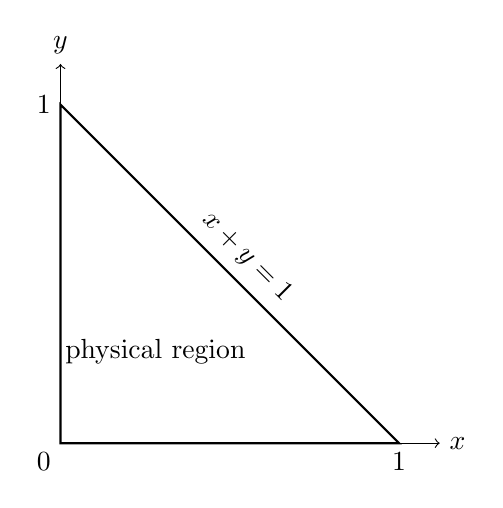
\begin{tikzpicture}[x=4.3cm,y=4.3cm]
  \draw[->] (0,0)--(1.12,0) node[right] {$x$};
  \draw[->] (0,0)--(0,1.12) node[above] {$y$};
  \draw[thick] (0,0)--(1,0)--(0,1)--cycle;
  \node[below left] at (0,0) {$0$};
  \node[below] at (1,0) {$1$};
  \node[left] at (0,1) {$1$};
  \node[rotate=-45,fill=white,inner sep=1pt] at (0.55,0.55) {$x+y=1$};
  \node at (0.28,0.27) {physical region};
\end{tikzpicture}
\end{center}
若截肢振幅在这个区域内近似为常数，三体相空间在 $(x,y)$ 平面上的事件密度就是常数，所以归一化后的二维密度为 $2$。任何明显的条带、边缘增强或局域峰都必须来自振幅本身的传播子、共振或角动量结构，而不是来自这个无质量三体测度的运动学边界。
\end{exbox}

\begin{derivation}[从\eqnrefs{eq:si-scattering-fourmomentum-r9}到\eqnrefs{eq:positive-energy-mass-shell-measure-r68}]
先从四维积分开始，并逐项检查其 Lorentz 变换性质：

\begin{equation*}
 I[F]\equiv
 \int\dd^4 p\,
 \delta(p^2-m^2c^2)\,\theta(p^0)F(p),
 \end{equation*}
其中 $\dd^4 p$ 的雅可比行列式在保向正时 Lorentz 变换下为 $1$，$p^2$ 是 Lorentz 标量，而这类变换保持 $p^0>0$。因此 $I[F]$ 对标量 $F$ 是 Lorentz 不变量。固定三动量后，把 $\delta$ 函数的自变量写成
\begin{equation*}
 f(p^0)=(p^0)^2-\mathbf p^2-m^2c^2.
\end{equation*}
两个根为 $p^0_\pm=\pm E_{\mathbf p}/c$，且
\begin{equation*}
 \left|\frac{\dd f}{\dd p^0}\right|_{p^0=p^0_\pm}
 =2\left|p^0_\pm\right|
 =\frac{2E_{\mathbf p}}{c}.
\end{equation*}
由一维恒等式
\begin{equation*}
 \delta[f(x)]
 =\sum_i\frac{\delta(x-x_i)}{|f'(x_i)|}
\end{equation*}
得到
\begin{equation*}
 \delta(p^2-m^2c^2)\theta(p^0)
 =\frac{c}{2E_{\mathbf p}}
 \delta\!\left(p^0-\frac{E_{\mathbf p}}{c}\right).
\end{equation*}
对 $p^0$ 积分以后，
\begin{equation*}
 I[F]
 =\int\frac{\dd^3 p}{2p^0}F(p)
 =\int\frac{c\,\dd^3 p}{2E_{\mathbf p}}F(p).
 \end{equation*}
左端是 Lorentz 不变量，因此右端就是正能质量壳上的不变量测度；完备关系~\eqnrefs{eq:rel-completeness-si-r9} 再按 Fourier 约定除以 $(2\pi\hbar)^3$。
\end{derivation}

\begin{derivation}[从\eqnrefs{eq:Ecm-s-si-r9}到\eqnrefs{eq:cm-momenta-kallen-si-r9}]
正文\eqnrefs{eq:Ecm-s-si-r9} 把质心总能量写成 $c\sqrt s$。在两体质心系中，两条粒子的三动量必定大小相同、方向相反，因此只剩一个未知的动量模。把两条质量壳条件与总能量守恒联立即可消去单粒子能量，得到正文\eqnrefs{eq:cm-momenta-kallen-si-r9}；根号何时变为实数同时给出二体阈值。

定义
\begin{equation*}
 \Lambda_K(a,b,c)=a^2+b^2+c^2-2ab-2ac-2bc.
 \end{equation*}
在初态质心系写
\begin{equation*}
 p_1^\mu=\left(\frac{E_1}{c},\mathbf p\right),
 \qquad
 p_2^\mu=\left(\frac{E_2}{c},-\mathbf p\right),
 \qquad
 c\sqrt s=E_1+E_2.
\end{equation*}
由
\begin{equation*}
 s=(p_1+p_2)^2=m_1^2c^2+m_2^2c^2+2p_1\!\cdot p_2
\end{equation*}
先得到
\begin{equation*}
 p_1\!\cdot p_2
 =\frac{s-(m_1^2+m_2^2)c^2}{2}.
\end{equation*}
另一方面
\begin{equation*}
 p_1\!\cdot p_2=\frac{E_1E_2}{c^2}+\mathbf p^2.
\end{equation*}
更直接的做法是先由 $P=p_1+p_2$ 与 $P^2=s$ 计算
\begin{align*}
 P\!\cdot p_1
 &=p_1^2+p_1\!\cdot p_2
 =\frac{s+(m_1^2-m_2^2)c^2}{2},\\
 P\!\cdot p_1
 &=\sqrt s\,\frac{E_1}{c},
\end{align*}
所以
\begin{equation*}
 E_1
 =\frac{c}{2\sqrt s}
 \left[s+(m_1^2-m_2^2)c^2\right].
\end{equation*}
再用 $E_1^2=m_1^2c^4+c^2p^2$，
\begin{align*}
 p^2
 &=\frac{1}{4s}
 \left[s+(m_1^2-m_2^2)c^2\right]^2-m_1^2c^2,\\
 &=\frac{\Lambda_K(s,m_1^2c^2,m_2^2c^2)}{4s}.
\end{align*}
因此
\begin{equation*}
 {
 |\mathbf p_i|
 =\frac{\sqrt{\Lambda_K(s,m_1^2c^2,m_2^2c^2)}}{2\sqrt s},
 \qquad
 |\mathbf p_f|
 =\frac{\sqrt{\Lambda_K(s,m_3^2c^2,m_4^2c^2)}}{2\sqrt s}.}
 \end{equation*}
末态阈值条件由根号非负给出 $c\sqrt s\ge(m_3+m_4)c^2$。
\end{derivation}

\begin{derivation}[从\eqnrefs{eq:phase2-si-start-r9}到\eqnrefs{eq:phase2-final-si-r9}]
正文\eqnrefs{eq:phase2-si-start-r9} 仍含两个末态三动量积分和一个四维守恒 $\delta$ 函数。在质心系中，三维 $\delta$ 函数先固定 $\mathbf p_4=-\mathbf p_3$，剩下的能量 $\delta$ 函数再固定径向动量模；最后只留下末态方向 $\dd\Omega$，从而得到正文\eqnrefs{eq:phase2-final-si-r9}。

采用能量四矢量
\begin{equation*}
 \mathcal P^\mu\equiv cp^\mu=(E,c\mathbf p),
 \end{equation*}
它只是物理四动量乘以常数 $c$。定义标准二体相空间因子
\begin{equation*}
 \dd\mathfrak P_2
 =(2\pi)^4\delta^{(4)}(\mathcal P_1+\mathcal P_2-\mathcal P_3-\mathcal P_4)
 \prod_{a=3,4}\frac{c^3\dd^3 p_a}{(2\pi)^3\,2E_a}.
 \end{equation*}
每个 $c^3\dd^3 p$ 都是 $\dd^3(c\mathbf p)$，所以 \eqnrefs{eq:phase2-si-start-r9} 完全由能量量纲的四动量组成。在质心系 $\mathcal P_1+\mathcal P_2=(c\sqrt s,\mathbf0)$。三维 $\delta$ 先令 $\mathbf p_4=-\mathbf p_3$，于是
\begin{equation*}
 \dd\mathfrak P_2
 =\frac{c^4p^2\dd p\,\dd\Omega}{(2\pi)^2 4E_3E_4}
 \delta(c\sqrt s-E_3-E_4).
\end{equation*}
令
\begin{equation*}
 f(p)=c\sqrt s-E_3(p)-E_4(p).
\end{equation*}
由 $\dd E_a/\dd p=c^2p/E_a$，
\begin{equation*}
 \left|f'(p)\right|
 =c^2p\left(\frac1{E_3}+\frac1{E_4}\right)
 =\frac{c^3p\sqrt s}{E_3E_4}.
\end{equation*}
所以
\begin{equation*}
 \delta[f(p)]
 =\frac{E_3E_4}{c^3p_f\sqrt s}\delta(p-p_f).
\end{equation*}
代回并积分 $p$，得到
\begin{equation*}
 {
 \dd\mathfrak P_2
 =\frac1{16\pi^2}\frac{|\mathbf p_f|}{\sqrt s}\,\dd\Omega.}
 \end{equation*}
右端无量纲，因为 $|\mathbf p_f|$ 与 $\sqrt s$ 都具有动量量纲。
\end{derivation}

\begin{derivation}[从\eqnrefs{eq:invariant-flux-scalar-r9}到\eqnrefs{eq:moller-velocity-si-r9}]
对两条入射轨迹，普通同一参考系中的相对相遇速率不能简单写成任意参考系都适用的 $|\mathbf v_1-\mathbf v_2|$。由四动量构造 Lorentz 标量

\begin{equation*}
 \mathcal I_{12}
 \equiv\sqrt{(p_1\!\cdot p_2)^2-m_1^2m_2^2c^4}.
 \end{equation*}
它具有动量平方量纲。定义 M\o ller 相对速率
\begin{equation*}
 v_{\rm M}
 \equiv
 \frac{c^3\mathcal I_{12}}{E_1E_2}.
 \end{equation*}
检查质心系时不跳过中间平方。写
\begin{equation*}
 p_1^\mu=\left(\frac{E_1}{c},\mathbf p_i\right),
 \qquad
 p_2^\mu=\left(\frac{E_2}{c},-\mathbf p_i\right),
\end{equation*}
于是
\begin{equation*}
 p_1\!\cdot p_2=\frac{E_1E_2}{c^2}+|\mathbf p_i|^2.
\end{equation*}
两条质量壳又分别给
\begin{equation*}
 m_a^2c^2=\frac{E_a^2}{c^2}-|\mathbf p_i|^2,
 \qquad a=1,2.
\end{equation*}
因此 \eqnrefs{eq:invariant-flux-scalar-r9} 根号中的量逐项化为
\begin{align*}
 \mathcal I_{12}^2
 &=\left(\frac{E_1E_2}{c^2}+p_i^2\right)^2
 -\left(\frac{E_1^2}{c^2}-p_i^2\right)
  \left(\frac{E_2^2}{c^2}-p_i^2\right),\\
 &=\frac{E_1^2E_2^2}{c^4}
 +\frac{2E_1E_2p_i^2}{c^2}+p_i^4
 -\frac{E_1^2E_2^2}{c^4}
 +\frac{(E_1^2+E_2^2)p_i^2}{c^2}-p_i^4,\\
 &=\frac{p_i^2}{c^2}(E_1+E_2)^2,
\end{align*}
其中 $p_i\equiv|\mathbf p_i|\ge0$。取正根得到
\begin{equation*}
 {
 \mathcal I_{12}
 =\frac{|\mathbf p_i|(E_1+E_2)}{c}
 =|\mathbf p_i|\sqrt s.}
 \end{equation*}
最后一步用了 $E_1+E_2=c\sqrt s$。于是
\begin{align*}
 v_{\rm M}
 &=|\mathbf p_i|c^2
 \left(\frac1{E_1}+\frac1{E_2}\right),\\
 &=|\mathbf v_1-\mathbf v_2|,
\end{align*}
因为 $\mathbf v_a=c^2\mathbf p_a/E_a$。所以 \eqnrefs{eq:moller-velocity-si-r9} 的协变表达确实回到熟悉的相对速度。
\end{derivation}

\begin{derivation}[从\eqnrefs{eq:delta-square-time-r15}到\eqnrefs{eq:2to2-cross-section-master-si-r9}]

取空间周期盒体积 $V$ 与观测时间 $T$。空间连续态满足
\begin{equation*}
 (2\pi\hbar)^3\delta^{(3)}(\mathbf0)=V,
 \qquad
 \sum_{\mathbf p}\longrightarrow
 V\int\frac{\dd^3 p}{(2\pi\hbar)^3}.
\end{equation*}
时间方向令 $\delta E\equiv E_f-E_i$，则
\begin{equation*}
 \int_{-T/2}^{T/2}\dd t\,\ee^{\ii\delta E t/\hbar}
 =T\,\operatorname{sinc}\!\left(\frac{\delta E T}{2\hbar}\right),
\end{equation*}
并由正文\eqnrefs{eq:delta-square-time-r15} 有
\begin{equation*}
 \lim_{T\to\infty}\frac1T
 \left|\int_{-T/2}^{T/2}\dd t\,\ee^{\ii\delta E t/\hbar}\right|^2
 =2\pi\hbar\delta(\delta E).
\end{equation*}
因此四维动量守恒 $\delta$ 函数平方在概率除以 $T$ 后留下一个能量守恒 $\delta$，其空间零点因子给出一个 $V$。结合两条初态的协变归一化，单位盒中单对入射粒子的二体末态跃迁率为正文\eqnrefs{eq:box-transition-rate-r15}，即
\begin{equation*}
 \dd\Gamma_{1+2\to2}
 =\frac{\hbar^2c^3}{4VE_1E_2}
 \overline{|\mathcal M|^2}\,\dd\mathfrak P_2.
\end{equation*}

单个归一化入射粒子在盒中的数密度是 $1/V$。正文\eqnrefs{eq:moller-velocity-si-r9} 给出相对速率，所以入射通量密度为
\begin{equation*}
 j_{12}=\frac{v_{\rm M}}{V}
 =\frac{c^3\mathcal I_{12}}{VE_1E_2}.
\end{equation*}
按正文中“跃迁率除以入射通量密度”的截面关系：
\begin{align*}
 \dd\sigma
 &=\frac{\dd\Gamma_{1+2\to2}}{j_{12}}\\
 &=\frac{\hbar^2}{4\mathcal I_{12}}
 \overline{|\mathcal M|^2}\,\dd\mathfrak P_2.
\end{align*}
$V$、$T$ 与参考系依赖的 $E_1E_2$ 在这一步全部消去。对 $2\to2$ 过程代入正文\eqnrefs{eq:phase2-final-si-r9}，并在质心系使用
$\mathcal I_{12}=|\mathbf p_i|\sqrt s$，得到
\begin{align*}
 \frac{\dd\sigma}{\dd\Omega}
 &=\frac{\hbar^2}{4|\mathbf p_i|\sqrt s}
 \overline{|\mathcal M|^2}
 \frac1{16\pi^2}\frac{|\mathbf p_f|}{\sqrt s}\\
 &=\frac{\hbar^2}{64\pi^2s}
 \frac{|\mathbf p_f|}{|\mathbf p_i|}
 \overline{|\mathcal M|^2},
\end{align*}
即正文\eqnrefs{eq:2to2-cross-section-master-si-r9}。
\end{derivation}

\begin{derivation}[从\eqnrefs{eq:delta-square-time-r15}到\eqnrefs{eq:master-decay-rate-si-r9}]
协变态归一化的单粒子初态在盒归一化后带因子 $(2P^0V)^{-1/2}$； 末态每条外腿给对应的质量壳测度。 LSZ 矩阵元中的四维 $\delta$ 在平方后，空间部分利用

\begin{equation*}
 (2\pi\hbar)^3\delta^{(3)}(\mathbf0)=V
\end{equation*}
消去母粒子的盒体积，而时间部分利用 \eqnrefs{eq:delta-square-time-r15} 把 $|\delta(E_f-E_i)|^2/T$ 化为单个能量 $\delta$。于是概率除以 $T$ 后只剩一个母粒子归一化因子 $1/(2P^0)$ 与 $n$ 体末态相空间。

为避免混淆能量量纲和动量量纲，先定义能量归一化截肢振幅
\begin{equation*}
 \mathcal A_E\equiv c\,\mathcal M.
\end{equation*}
若 $\mathcal M$ 在某个过程具有一个动量量纲，则 $\mathcal A_E$ 具有能量量纲。有限盒推导给
\begin{equation*}
 \dd\Gamma_{1\to n}
 =\frac{1}{2E_P\hbar}\,
 \overline{|\mathcal A_E|^2}\,\dd\mathfrak P_n,
 \qquad E_P=Mc^2.
 \end{equation*}
把 $\mathcal A_E=c\mathcal M$ 与 $E_P=Mc^2$ 代入，两个 $c^2$ 消去：
\begin{align*}
 \dd\Gamma_{1\to n}
 &=\frac{c^2}{2Mc^2\hbar}
 \overline{|\mathcal M|^2}\,\dd\mathfrak P_n,\\
 &={
 \frac{1}{2M\hbar}
 \overline{|\mathcal M|^2}\,\dd\mathfrak P_n.}
 \end{align*}
这里 $\dd\mathfrak P_n$ 使用能量四矢量 $\mathcal P^\mu=cp^\mu$ 的定义。以无量纲 Yukawa 耦合的费米子对衰变为例，振幅含有双线性因子 $\bar u v$；在上述外腿归一化下该双线性具有动量量纲，因此
\begin{equation*}
 \left[\frac{|\mathcal M|^2}{M\hbar}\right]
 =\mathrm{s^{-1}},
\end{equation*}
与衰变率的 SI 单位一致。这样 \eqnrefs{eq:master-decay-rate-si-r9} 与散射截面主式共享同一套有限盒、有限时间和外腿归一化，而不是独立记忆的另一条规则。
\end{derivation}



\begin{derivation}[从\eqnrefs{eq:phase3-definition-dp68}到\eqnrefs{eq:phase3-recursive-dp52}]
正文\eqnrefs{eq:phase3-definition-dp68} 是三体末态的原始 Lorentz 不变测度。内部不变质量 $\mathcal S_{12}$ 可以作为显式积分变量。引入 $\mathcal Q_{12}=\mathcal P_1+\mathcal P_2$，并插入

\begin{align*}
1
={}&\int\dd^4 \mathcal Q_{12}\,
\delta^{(4)}(\mathcal Q_{12}-\mathcal P_1-\mathcal P_2)\\
&\times\int\dd\mathcal S_{12}\,
\delta(\mathcal Q_{12}^2-\mathcal S_{12})\theta(\mathcal Q_{12}^0).
\end{align*}
正能质量壳恒等式
\begin{equation*}
\delta(\mathcal Q_{12}^2-\mathcal S_{12})\theta(\mathcal Q_{12}^0)
=\frac{1}{2E_{12}}\delta(\mathcal Q_{12}^0-E_{12})
\end{equation*}
把 $\mathcal Q_{12}$ 的四维积分化成标准单粒子质量壳测度。重新组合总四动量 $\delta$ 函数与三条末态测度后得到
\begin{align*}
\dd\mathfrak P_3
={}&\frac{\dd\mathcal S_{12}}{2\pi}
\left[\dd\mathfrak P_2(P;q_{12},3)\right]
\left[\dd\mathfrak P_2(q_{12};1,2)\right],
\end{align*}
这就是正文\eqnrefs{eq:phase3-recursive-dp52}。中间四动量 $q_{12}=p_1+p_2$ 仅用于把同一组三体末态按 $(12)+3$ 分组；其不变量 $q_{12}^2=\mathcal S_{12}$ 是三体相空间积分变量。
\end{derivation}

\begin{derivation}[从\eqnrefs{eq:phase3-recursive-dp52}到\eqnrefs{eq:phase3-dalitz-dp52}]
在母粒子静止系中，对正文\eqnrefs{eq:phase3-recursive-dp52} 的两个二体因子分别使用\eqnrefs{eq:phase2-final-si-r9}：

\begin{equation*}
\dd\mathfrak P_3
=\frac{\dd\mathcal S_{12}}{2\pi}
\frac{1}{16\pi^2}\frac{|\mathbf p_3|}{Mc}\dd\Omega_3
\frac{1}{16\pi^2}\frac{|\mathbf p_2^*|}{\sqrt{\mathcal S_{12}}/c}\dd\Omega_2^*.
\end{equation*}
若母粒子无自旋或已做自旋平均，整体方向积分给 $\int\dd\Omega_3=4\pi$。在 $q_{12}$ 静止系中以粒子 3 为极轴，方位角再给 $2\pi$，于是
\begin{equation*}
\dd\mathfrak P_3
=\frac{\dd\mathcal S_{12}\,\dd\cos\theta^*}{64\pi^3}
\frac{|\mathbf p_3|}{Mc}
\frac{|\mathbf p_2^*|}{\sqrt{\mathcal S_{12}}/c}.
\end{equation*}
正文\eqnrefs{eq:dalitz-angular-map-dp68} 给出
\begin{equation*}
\left|\frac{\partial\mathcal S_{23}}{\partial\cos\theta^*}\right|
=2c^2|\mathbf p_2^*||\mathbf p_3^*|.
\end{equation*}
因此把 $\cos\theta^*$ 换成 $\mathcal S_{23}$ 时，两个动量模恰好与 Jacobian 相消；再用 $\sqrt{\mathcal S_{12}}$ 和母粒子质量整理剩余因子，得到
\begin{equation*}
\dd\mathfrak P_3
=\frac{\dd\mathcal S_{12}\,\dd\mathcal S_{23}}{128\pi^3M^2c^4},
\end{equation*}
即正文\eqnrefs{eq:phase3-dalitz-dp52}。
\end{derivation}

\begin{derivation}[从\eqnrefs{eq:dalitz-angular-map-dp68}到\eqnrefs{eq:dalitz-boundary-dp52}]
在 $q_{12}$ 静止系中，两次二体运动学分别给

\begin{align*}
E_2^*
&=\frac{\mathcal S_{12}+m_2^2c^4-m_1^2c^4}{2\sqrt{\mathcal S_{12}}},\\
E_3^*
&=\frac{M^2c^4-\mathcal S_{12}-m_3^2c^4}{2\sqrt{\mathcal S_{12}}},\\
c|\mathbf p_2^*|
&=\frac{\sqrt{\Lambda_K(\mathcal S_{12},m_1^2c^4,m_2^2c^4)}}{2\sqrt{\mathcal S_{12}}},\\
c|\mathbf p_3^*|
&=\frac{\sqrt{\Lambda_K(M^2c^4,\mathcal S_{12},m_3^2c^4)}}{2\sqrt{\mathcal S_{12}}}.
\end{align*}
把这些量代入正文\eqnrefs{eq:dalitz-angular-map-dp68}。由于 $\mathcal S_{23}$ 对 $\cos\theta^*$ 是线性的，固定 $\mathcal S_{12}$ 时的最大值与最小值必定出现在 $\cos\theta^*=\mp1$。逐项代入便得到正文\eqnrefs{eq:dalitz-boundary-dp52}。

两个 Källén 根号还必须同时为实数，因此
\begin{equation*}
(m_1+m_2)^2c^4
\le\mathcal S_{12}
\le(M-m_3)^2c^4.
\end{equation*}
这给出 Dalitz 区域在 $\mathcal S_{12}$ 方向上的完整阈值范围。
\end{derivation}


\subsection{交叉与色散}
同一个截肢核在不同外态指派下产生交叉过程；解析性又把不同能区的实部、虚部和阈值连接起来。因而交叉不是“换符号口诀”，色散关系也不是独立技巧，而是同一复解析振幅的两种读取方式。
LSZ 约化把时序关联函数转化为实验散射振幅以后，同一个解析振幅还包含比单一反应道更多的信息。改变某条外腿的入射/出射解释会把散射、湮灭和对产生联系起来；真实中间态打开后出现的虚部，则通过复解析性约束阈值以下的实部。前者由交叉关系描述，后者由色散关系描述。

第一个问题的答案来自外腿的解析延拓。LSZ 振幅取自同一个截肢关联函数，只是不同物理过程把不同外腿解释为入射粒子、出射粒子或相应反粒子。改变这种解释时，四动量的符号和外线波函数必须一起改变。这一关系称为\emph{交叉}。

第二个问题来自复变量解析性。虚中间态尚不能处在真实质量壳上时，振幅可以平滑地随运动学变量变化；一旦某个真实多粒子通道打开，振幅在相应阈值处出现分支点，实轴两侧的边界值不再相同。这个差值就是割线不连续度，它的虚部由真实在壳中间态决定。若振幅在割线之外解析，Cauchy 公式便把这些边界值与其它运动学区域联系起来；为了控制高能端的积分，必要时要做有限次减法。这就是色散关系的来源。


交叉关系最清楚的记号是把四点截肢连通核统一写成“所有四动量均流入顶角”的形式
\begin{equation}
 \mathcal A(p_1,p_2,p_3,p_4),
 \qquad
 p_1+p_2+p_3+p_4=0.
 \label{eq:all-incoming-amplitude-dp9}
\end{equation}
对物理过程 $1+2\to3+4$，$p_1,p_2,p_3,p_4$ 都取正能物理四动量；出射外腿在全入射核中必须反向，因此
\begin{equation}
 \boxed{
 \mathcal M_{12\to34}
 =\mathcal A(p_1,p_2,-p_3,-p_4).}
 \label{eq:physical-from-all-incoming-dp9}
\end{equation}
若把某条外腿改解释为交叉过程中的反粒子，不能只机械地把 Mandelstam 变量换名；必须同时解析延拓该外腿四动量，并把 Dirac 外线的 $u$、$v$ 或矢量场的偏振波函数换成新物理态对应的外线因子。这个联合替换才保持同一截肢核与不同物理外态之间的对应。

\begin{note}[交叉关系的使用范围]
在逐阶微扰展开中，外腿延拓可直接作用于 Feynman 图的解析表达式。完全非微扰的交叉定理还依赖局域性、谱条件和解析延拓的全局性质。\eqnrange{eq:all-incoming-amplitude-dp9}{eq:physical-from-all-incoming-dp9} 所用的是标准局域量子场论中的外腿交叉规则，而不是对任意非局域模型的无条件恒等式。
\end{note}

转向第二个问题。固定其它运动学变量，把待研究的振幅或形状因子记作复变量 $z$ 的函数 $F(z)$。这里 $z$ 可取某个 Mandelstam 不变量，因而具有动量平方量纲。真实中间态通常从某个右手阈值 $s_R$ 开始产生割线；交叉道可以在负实轴方向产生左手割线，其最高端点记为 $s_L$。在两条割线之间选一个解析点 $z_0$ 作为减法点。

减法的目的很具体：如果 $F(z)$ 在无穷远衰减得不够快，就不能直接丢掉 Cauchy 大圆。取整数 $N\ge1$，用 $F$ 在 $z_0$ 的前 $N$ 阶 Taylor 数据构造
\begin{equation}
 \boxed{
 H_N(\zeta;z)
 \equiv
 \frac{
 F(\zeta)-\displaystyle\sum_{r=0}^{N-1}
 \frac{F^{(r)}(z_0)}{r!}(\zeta-z_0)^r
 }
 {(\zeta-z_0)^N(\zeta-z)}.}
 \label{eq:subtracted-cauchy-kernel-dp68}
\end{equation}
只要 $N$ 取得足够大，使 $H_N$ 在无穷远大圆上的积分消失，就可以把闭合轮廓收缩到实轴割线和孤立极点。于是得到 $N$ 次减法色散关系
\begin{equation}
 \boxed{
 \begin{aligned}
 F(z)
 &=\sum_{r=0}^{N-1}
 \frac{F^{(r)}(z_0)}{r!}(z-z_0)^r
 +\frac{(z-z_0)^N}{\pi}
 \int_{s_R}^{\infty}\!\dd s'\,
 \frac{\operatorname{Im}F(s'+\ii0^+)}{(s'-z_0)^N(s'-z)}
 \\
 &\quad
 +\frac{(z-z_0)^N}{\pi}
 \int_{-\infty}^{s_L}\!\dd s'\,
 \frac{\operatorname{Im}F(s'+\ii0^+)}{(s'-z_0)^N(s'-z)}
 +\text{孤立极点项}.
 \end{aligned}}
 \label{eq:general-subtracted-dispersion-dp9}
\end{equation}
这里的减法多项式由 $F(z_0),F'(z_0),\ldots$ 这样的低能输入或重整化条件确定；割线积分则来自真实中间态。二者的物理来源不同，不能把减法常数误认为由幺正性自动决定。

若只有从 $s_0$ 开始的右手割线，并取一次减法 $N=1$、$z_0=0$ 且 $F(0)=0$，\eqnrefs{eq:general-subtracted-dispersion-dp9} 退化为
\begin{equation}
 \boxed{
 F(z)
 =\frac{z}{\pi}
 \int_{s_0}^{\infty}\dd s'\,
 \frac{\operatorname{Im}F(s'+\ii0^+)}{s'(s'-z)}.}
 \label{eq:once-subtracted-single-cut-dp9}
\end{equation}
例如在真空极化中，时间样区域的真实 $e^-e^+$ 产生决定 $\operatorname{Im}F$，同一色散积分据此重建类空区域的实部。

对某些由光学定理保证谱权重 $\rho(s)\equiv\operatorname{Im}F(s+\ii0^+)\ge0$ 的标量投影，\eqnrefs{eq:once-subtracted-single-cut-dp9} 还给出一个直接的符号检查。令 $z=-Q^2<0$，只要相应谱矩收敛，就有
\begin{equation}
 \boxed{
 (-1)^n\frac{\dd^n}{\dd(Q^2)^n}F(-Q^2)\ge0,
 \qquad n\ge1.}
 \label{eq:spacelike-spectral-positivity-dp68}
\end{equation}
这不是任意振幅都满足的额外公理；它只适用于当前投影的谱密度确实非负的情形。

交叉关系与色散关系连接散射振幅的两个不同层面：前者把不同外态过程识别为同一截肢关联函数在不同质量壳边界上的取值，后者用割线虚部和必要的减法常数重建解析域中的其余部分。具体理论只需要把相应粒子质量、耦合与传播子代入这些一般结构。


\begin{derivation}[从\eqnrefs{eq:all-incoming-amplitude-dp9}到\eqnrefs{eq:physical-from-all-incoming-dp9}]
全入射约定把每一条外腿的四动量都定义成指向相互作用区。设全入射核的四个参数为 $k_i$，则正文\eqnrefs{eq:all-incoming-amplitude-dp9} 要求
\[
k_1+k_2+k_3+k_4=0.
\]
对物理过程 $1+2\to3+4$，实验四动量满足
\[
p_1+p_2=p_3+p_4.
\]
前两条腿本来就流入，所以
\[
k_1=p_1,\qquad k_2=p_2.
\]
末态 3、4 的物理箭头流出相互作用区；若仍要求 $k_i$ 全部向内，必须反号：
\[
k_3=-p_3,\qquad k_4=-p_4.
\]
于是全入射的动量守恒自动变成
\begin{align*}
k_1+k_2+k_3+k_4
&=p_1+p_2-p_3-p_4\\
&=0,
\end{align*}
与物理守恒完全一致。将四个 $k_i$ 代回同一个截肢四点核，便得到正文\eqnrefs{eq:physical-from-all-incoming-dp9}：
\[
\mathcal M_{12\to34}
=\mathcal A(p_1,p_2,-p_3,-p_4).
\]
\end{derivation}

\begin{derivation}[从\eqnrefs{eq:subtracted-cauchy-kernel-dp68}到\eqnrefs{eq:general-subtracted-dispersion-dp9}]
把轮廓收缩到两条实轴割线。实解析性给出

\begin{equation*}
 F(s'-\ii0^+)=F(s'+\ii0^+)^*,
\end{equation*}
所以割线两侧的差为
\begin{equation*}
 \operatorname{Disc}F(s')
 \equiv F(s'+\ii0^+)-F(s'-\ii0^+)
 =2\ii\operatorname{Im}F(s'+\ii0^+).
\end{equation*}
右手割线因此贡献
\begin{equation*}
 \frac{(z-z_0)^N}{\pi}
 \int_{s_R}^{\infty}\!\dd s'\,
 \frac{\operatorname{Im}F(s'+\ii0^+)}
 {(s'-z_0)^N(s'-z)},
\end{equation*}
左手割线同理给出从 $-\infty$ 到 $s_L$ 的积分。最后把预先减去的 Taylor 多项式加回，并把轮廓内未并入割线的孤立极点留作显式留数项，就得到正文\eqnrefs{eq:general-subtracted-dispersion-dp9}。

若 $z$ 逼近割线，分母 $1/(s'-z)$ 按 $z\to z+\ii0^+$ 理解。其主值部分给出实部，跨越极点产生的 $\ii\pi$ 项恢复原来的虚部，因此色散式同时编码了割线两侧的完整边界值。
\end{derivation}



\begin{derivation}[从\eqnrefs{eq:once-subtracted-single-cut-dp9}到\eqnrefs{eq:spacelike-spectral-positivity-dp68}]
这一结论只讨论谱密度 $\rho(s)\equiv\operatorname{Im}F(s+\ii0^+)\ge0$ 的投影。令 $z=-Q^2$、$Q^2>0$，正文\eqnrefs{eq:once-subtracted-single-cut-dp9} 变为
\begin{equation*}
F(-Q^2)
=-\frac{Q^2}{\pi}
\int_{s_0}^{\infty}\dd s'\,
\frac{\rho(s')}{s'(s'+Q^2)}.
\end{equation*}
利用恒等式
\begin{equation*}
\frac{Q^2}{s'(s'+Q^2)}
=\frac1{s'}-\frac1{s'+Q^2},
\end{equation*}
可以把所有 $Q^2$ 依赖集中到第二项：
\begin{equation*}
F(-Q^2)
=-\frac1\pi\int_{s_0}^{\infty}\frac{\rho(s')}{s'}\dd s'
+\frac1\pi\int_{s_0}^{\infty}\frac{\rho(s')}{s'+Q^2}\dd s'.
\end{equation*}
若相应谱矩收敛，可以逐次把 $Q^2$ 导数移入积分号。一次和二次导数分别为
\begin{align*}
\frac{\dd}{\dd Q^2}F(-Q^2)
&=-\frac1\pi\int_{s_0}^{\infty}\dd s'\,
\frac{\rho(s')}{(s'+Q^2)^2}\le0,\\
\frac{\dd^2}{\dd(Q^2)^2}F(-Q^2)
&=\frac{2}{\pi}\int_{s_0}^{\infty}\dd s'\,
\frac{\rho(s')}{(s'+Q^2)^3}\ge0.
\end{align*}
继续求导时，每次只会再产生一个负号和一个正的整数系数，因此归纳得到正文\eqnrefs{eq:spacelike-spectral-positivity-dp68}。它给出了一个很实用的自洽检查：若显式圈积分声称对应同一非负谱投影，却违反这一导数符号层级，就说明符号、减法或解析延拓中至少有一处不一致。
\end{derivation}



\subsection{标量散射实验室}
最简单的标量相互作用已经足以同时产生图、振幅、衰变率、截面与静态势，并且不引入自旋和规范自由度。它因此隔离出散射论本身的运动学、相空间与解析结构；自旋和规范代数只在更复杂的费米子与光子模型中加入。
% -----------------------------------------------------------------------------
% Scalar-only reduced momentum-space rules in strict SI units
% -----------------------------------------------------------------------------

LSZ 给出的物理场 Green 函数在标量散射中可整理为一组约化图因子。“约化”表示把每张图中重复出现的 SI 场归一化常数统一提出；四动量采用物理动量量纲，SI 归一化常数显式保留在 Green 函数与外线因子中。

质量为 $m$ 的实标量场，其动量-空间 Feynman 二点函数已由正则量子化得到
\begin{equation}
 \widetilde\Delta_F(p)
 =\frac{\ii\hbar^3c}{p^2-m^2c^2+\ii0^+}.
 \label{eq:scalar-physical-propagator-common-r15}
\end{equation}
分子 $\hbar^3c$ 来自采用的 SI 场归一化与 Fourier 约定；极点的位置 $p^2=m^2c^2$ 和 $+\ii0^+$ 边界条件与这个共同常数无关。因此定义标量约化内部线
\begin{equation}
 \boxed{
 \Delta_{\rm red}(p)
 \equiv\frac{\ii}{p^2-m^2c^2+\ii0^+}.}
 \label{eq:scalar-reduced-propagator-common-r15}
\end{equation}
它的 SI 量纲是物理动量的负二次方。这个定义不会把质量 $m$ 当成动量；分母中必须写 $m^2c^2$。


对实标量场 $\varphi$，把四次相互作用写成
\begin{equation}
 \boxed{
 \Lag_{\varphi^4}^{\rm int}
 =-\frac{g_4}{4!\,\hbar c}\varphi^4,}
 \qquad [g_4]=1.
 \label{eq:phi4-si-coupling-common-r15}
\end{equation}
由于 $[\varphi]=\sqrt{\mathrm{J/m}}$，有 $[\varphi^4]=\mathrm{J^2/m^2}$，而 $[\hbar c]=\mathrm{J\,m}$，所以右端确实具有拉格朗日密度的 SI 单位 $\mathrm{J/m^3}$。Dyson 插入与 LSZ 外腿截肢合并后，一个约化 $\varphi^4$ 顶角留下 $-\ii g_4$；这与 \eqnrefs{eq:phi4-lsz-result-r7} 的 SI 归一化完全一致。


% -----------------------------------------------------------------------------
% Full scalar-interaction laboratory in strict SI units
% -----------------------------------------------------------------------------

复标量物质场与实标量媒介场提供了不含自旋指标的最小散射模型。在这个体系中，作用量、Dyson 展开、Wick 收缩、LSZ 截肢、散射振幅、相空间和截面可以在同一套归一化下完整闭合。四动量继续采用全书的 SI 约定
\begin{equation*}
 p^\mu=(E_{\mathbf p}/c,\mathbf p),\qquad p^2=m_{\rm ch}^2c^2,
\end{equation*}
质量通过质壳条件进入能量--动量关系。复标量的质量记为 $m_{\rm ch}$，实媒介粒子的静质量记为 $m_\chi$；$m_\chi$ 的 SI 单位为 $\mathrm{kg}$。

由标量场作用量的 SI 归一化有 $[\varphi_{\rm ch}]=[\chi]=\sqrt{\mathrm{J/m}}$。因此三次单项式 $\varphi_{\rm ch}^\dagger\varphi_{\rm ch}\chi$ 的系数不能写成一个无量纲常数。定义具有\emph{动量量纲}的约化三次耦合 $g_3$，并写
\begin{equation}
 \boxed{
 \Lag_{3}
 =-\frac{g_3}{\hbar\sqrt{\hbar c}}\,\varphi_{\rm ch}^\dagger\varphi_{\rm ch}\chi,}
 \qquad [g_3]=\mathrm{kg\,m\,s^{-1}}.
 \label{eq:scalar-cubic-si-r10}
\end{equation}
量纲可逐项检查：$[\hbar\sqrt{\hbar c}]=\mathrm{kg^{3/2}m^{7/2}s^{-2}}$，所以 $[g_3/(\hbar\sqrt{\hbar c})]=\mathrm{J^{-1/2}m^{-3/2}}$；再乘 $[\varphi_{\rm ch}^\dagger\varphi_{\rm ch}\chi]=\mathrm{J^{3/2}m^{-3/2}}$，正好得到 $\mathrm{J/m^3}$。

\begin{exbox}[$\chi\to\varphi_{\rm ch}+\varphi_{\rm ch}^{\ast}$ 的两体衰变]
取母媒介粒子的四动量为 $p_\chi$，末态四动量为 $p_1,p_2$：
\begin{equation*}
 p_\chi=p_1+p_2,\qquad p_\chi^2=m_\chi^2c^2,\qquad p_1^2=p_2^2=m_{\rm ch}^2c^2.
\end{equation*}
只有一个顶角，所以约化振幅为
\begin{equation}
 \ii\mathcal M=-\ii g_3,
 \qquad |\mathcal M|^2=g_3^2.
 \label{eq:scalar-cubic-decay-mphi-r15}
\end{equation}
在母粒子静止系，
\begin{equation*}
 p_\chi^\mu=(m_\chi c,\mathbf0),\qquad
 p_1^\mu=(E/c,\mathbf p),\qquad
 p_2^\mu=(E/c,-\mathbf p).
\end{equation*}
能量守恒给 $2E=m_\chi c^2$。再用 $E^2=m_{\rm ch}^2c^4+c^2p^2$，
\begin{align*}
 p^2
 &=\frac{E^2}{c^2}-m_{\rm ch}^2c^2,\\
 &=\frac{m_\chi^2c^2}{4}-m_{\rm ch}^2c^2,
\end{align*}
所以
\begin{equation}
 \boxed{
 |\mathbf p|
 =\frac{c}{2}\sqrt{m_\chi^2-4m_{\rm ch}^2},
 \qquad m_\chi\ge 2m_{\rm ch}.}
 \label{eq:scalar-cubic-decay-p-r10}
\end{equation}
使用由 Lorentz 不变量二体相空间得到的一体衰变公式 \eqnrefs{eq:master-decay-rate-si-r9}，并代入
\begin{equation*}
 \int\dd\mathfrak P_2
 =\frac{|\mathbf p|}{4\pi m_\chi c},
\end{equation*}
得到
\begin{align}
 \Gamma_{\chi\to\varphi_{\rm ch}\varphi_{\rm ch}^{\ast}}
 &=\frac{1}{2m_\chi\hbar}g_3^2
 \frac{|\mathbf p|}{4\pi m_\chi c},\\
 &=\boxed{
 \frac{g_3^2}{16\pi m_\chi\hbar}
 \sqrt{1-\frac{4m_{\rm ch}^2}{m_\chi^2}}.}
 \label{eq:scalar-cubic-decay-width-r10}
\end{align}
量纲检查为 $[g_3^2/(m_\chi\hbar)]=\mathrm{s^{-1}}$。末态粒子与反粒子可区分，所以没有 $1/2!$；若两个末态是同种实标量，相空间必须再除以 $2!$。


\medskip

\eqnrefs{eq:scalar-cubic-si-r10} 已固定三次相互作用的 SI 归一化。取 Dyson 展开的最低非零阶，把三条外腿接到同一个局域插入点，并按 LSZ 约定截去外腿传播子，就得到\eqnrefs{eq:scalar-cubic-decay-mphi-r15} 中的约化顶角振幅。这里三种场在顶角上彼此可区分，因此不存在额外的 $3!$ 组合因子。

相互作用绘景散射算符的一阶项为
\begin{align*}
\hat S_3^{(1)}
&=\frac{\ii}{\hbar c}\int\dd^4 x\,\Lag_3(x)\\
&=-\frac{\ii g_3}{\hbar^2c\sqrt{\hbar c}}
\int\dd^4 x\,
\varphi_{\rm ch}^\dagger(x)\varphi_{\rm ch}(x)\chi(x).
\end{align*}
把一条 $\varphi_{\rm ch}$、一条 $\varphi_{\rm ch}^\ast$ 和一条 $\chi$ 外腿接到该插入点，树级连通三点函数的极点部分为
\begin{align*}
\widetilde G_{3,c}^{(1)}
={}&(2\pi\hbar)^4\delta^{(4)}(p_\chi-p_1-p_2)
\left(-\frac{\ii g_3}{\hbar^2c\sqrt{\hbar c}}\right)\\
&\times
\widetilde\Delta_{\rm ch}(p_1)
\widetilde\Delta_{\rm ch}(p_2)
\widetilde\Delta_\chi(p_\chi),
\end{align*}
其中
\begin{equation*}
\widetilde\Delta_a(p)
=\frac{\ii\hbar^3c}{p^2-m_a^2c^2+\ii0^+}.
\end{equation*}
树级留数为 $Z_a=1$。对三条外腿分别乘相应逆极点因子并取质量壳极限，三个传播子全部消去，留下
\begin{equation*}
\ii\mathfrak A_3
=-\frac{\ii g_3}{\hbar^2c\sqrt{\hbar c}}.
\end{equation*}
按照约化标量振幅的定义
$\mathcal M_3\equiv\hbar^2c\sqrt{\hbar c}\,\mathfrak A_3$，于是
\begin{equation*}
\ii\mathcal M_3=-\ii g_3,
\end{equation*}
即\eqnrefs{eq:scalar-cubic-decay-mphi-r15} 的第一式。
\end{exbox}

在同一三次耦合理论中，若两种可区分物质场 $\varphi_{{\rm ch},A}$、$\varphi_{{\rm ch},B}$ 分别以 $g_{3A}$、$g_{3B}$ 耦合到同一中性媒介场 $\chi$，最低阶弹性过程
\[
A(p_1)+B(p_2)\to A(p_3)+B(p_4)
\]
由一条 $t$ 道媒介传播线连接两个三点顶角。令交换四动量 $q=p_1-p_3$、$t=q^2$，则树级约化振幅为
\begin{equation}
\boxed{
\mathcal M_t
=\frac{g_{3A}g_{3B}}{m_\chi^2c^2-t}.}
\label{eq:scalar-exchange-mphi-r15}
\end{equation}
分母直接记录媒介传播子的极点位置；$g_{3A}g_{3B}$ 与分母具有相同的动量平方量纲，因此 $\mathcal M_t$ 无量纲。它同时决定相对论散射截面和低速极限中的有效势，两者只是同一交换核在不同运动学区域的读出。

\begin{exbox}[单媒介粒子交换的角分布]
取 $m_A,m_B$ 为两种物质粒子的质量。由正文\eqnrefs{eq:scalar-exchange-mphi-r15}，标量外腿没有自旋求和，故
\begin{equation}
 \boxed{
 \overline{|\mathcal M_t|^2}
 =\frac{g_{3A}^2g_{3B}^2}{(m_\chi^2c^2-t)^2}.}
 \label{eq:scalar-exchange-M2-r10}
\end{equation}
对等质量弹性散射 $m_A=m_B=m_{\rm ch}$，质心系
\begin{equation*}
 s=4(m_{\rm ch}^2c^2+p^2),\qquad
 t=-2p^2(1-\cos\theta),
\end{equation*}
而 $p_f=p_i$。代入 SI 截面主式，
\begin{equation}
 \boxed{
 \frac{\dd\sigma}{\dd\Omega}
 =\frac{\hbar^2}{64\pi^2s}
 \frac{g_{3A}^2g_{3B}^2}
 {[m_\chi^2c^2+2p^2(1-\cos\theta)]^2}.}
 \label{eq:scalar-exchange-angular-r10}
\end{equation}
这里 $\hbar^2/s$ 提供面积量纲，因此该因子必须保留在 SI 截面中。
\end{exbox}

交换振幅还可以回答一个与截面不同的问题：当两粒子运动足够慢、能量转移远小于空间动量转移时，这个相对论交换过程能否被一个定态势能描述？这个问题不能只看传播子分母的形状，因为相对论外态与 Schr\"odinger 两体态采用不同归一化。需要先把同一个低速散射截面在两种描述中匹配，再把动量空间核 Fourier 变换到坐标空间。

令
\begin{equation*}
 m_{\rm red}\equiv\frac{m_A m_B}{m_A+m_B},
 \qquad
 \kappa\equiv\frac{p}{\hbar},
\end{equation*}
分别表示两体相对运动的约化质量与波数。定态 Schr\"odinger 方程可写成 Helmholtz 形式
\begin{equation}
 (\nabla^2+\kappa^2)\psi(\mathbf r)
 =\frac{2m_{\rm red}}{\hbar^2}V(\mathbf r)\psi(\mathbf r),
 \label{eq:sch-helmholtz-r13}
\end{equation}
其出射 Green 核 $G_0^{(+)}$ 给出 Lippmann--Schwinger 方程
\begin{equation}
 \psi(\mathbf r)=\ee^{\ii\boldsymbol\kappa_i\cdot\mathbf r}
 -\frac{2m_{\rm red}}{\hbar^2}\int\dd^3 r'\,
 G_0^{(+)}(\mathbf r-\mathbf r')V(\mathbf r')\psi(\mathbf r').
 \label{eq:sch-lippmann-r13}
\end{equation}
在 $|q^0|/|\mathbf q|\ll1$ 与 $|\mathbf p|/(m_{A,B}c)\ll1$ 的静态低速区间，相对论外态与 Schr\"odinger 两体态的归一化必须先统一。对可区分的弹性二体通道，在前文固定的 $S$ 矩阵、相空间与空间 Fourier 约定下，若 $\mathcal M_{\rm rel}^{\rm NR}(\mathbf q)$ 表示相对论约化振幅的低速矩阵元，则通用匹配关系为
\begin{equation}
\boxed{
\widetilde V_{\rm NR}(\mathbf q)
=-\frac{\hbar^3}{4m_A m_Bc}\,
\mathcal M_{\rm rel}^{\rm NR}(\mathbf q).}
\label{eq:relativistic-to-nr-potential-matching-dp75}
\end{equation}
这里 $\widetilde V_{\rm NR}$ 是对空间坐标作 Fourier 变换得到的势核，量纲为 $\mathrm{J\,m^3}$；若振幅仍含自旋指标，\eqnrefs{eq:relativistic-to-nr-potential-matching-dp75} 按固定自旋通道理解为势算符的矩阵元。这个关系只属于低速、近静态、弹性的一体势描述，不适用于显著能量转移、实粒子产生或不可忽略迟滞的区域。

对当前标量交换，\eqnrefs{eq:scalar-exchange-mphi-r15} 在该极限变成
$\mathcal M_{\rm rel}^{\rm NR}=g_{3A}g_{3B}/(\mathbf q^2+m_\chi^2c^2)$，故\eqnrefs{eq:relativistic-to-nr-potential-matching-dp75} 立即给出
\begin{equation}
 \boxed{
 \widetilde V_{\rm NR}(\mathbf q)
 =-\frac{\hbar^3g_{3A}g_{3B}}{4m_A m_Bc}
 \frac{1}{\mathbf q^2+m_\chi^2c^2}.}
 \label{eq:scalar-yukawa-momentum-kernel-dp68}
\end{equation}
再按全书空间 Fourier 约定变回坐标空间，得到
\begin{equation}
 \boxed{
 V_Y(r)=-\alpha_{AB}^{(s)}\frac{\hbar c}{r}\ee^{-r/\lambda_\chi},
 \qquad
 \alpha_{AB}^{(s)}\equiv\frac{g_{3A}g_{3B}}{16\pi m_A m_Bc^2},
 \qquad
 \lambda_\chi\equiv\frac{\hbar}{m_\chi c}.}
 \label{eq:scalar-yukawa-potential-dp49}
\end{equation}
无量纲 $\alpha_{AB}^{(s)}$ 控制势强度，$\lambda_\chi$ 是媒介粒子的 Compton 长度并控制作用程。$m_\chi\to0$ 时 $\lambda_\chi\to\infty$，屏蔽因子消失；因此有质量传播子的极点位置经三维 Fourier 变换直接生成指数屏蔽与有限作用程。
同一三次顶角允许
\begin{equation*}
 \chi(p_\chi)+\varphi_{\rm ch}(p)\to\chi(p_\chi')+\varphi_{\rm ch}(p').
\end{equation*}
两条外部 $\chi$ 沿物质线有两种次序，因此内部物质线四动量分别为 $p+p_\chi$ 与 $p-p_\chi'$。约化振幅是
\begin{equation}
 \boxed{
 \mathcal M
 =g_3^2\left[
 \frac1{(p+p_\chi)^2-m_{\rm ch}^2c^2+\ii0^+}
 +\frac1{(p-p_\chi')^2-m_{\rm ch}^2c^2+\ii0^+}
 \right].}
 \label{eq:scalar-compton-analogue-si-r10}
\end{equation}
由 $p^2=p'^2=m_{\rm ch}^2c^2$、$p_\chi^2=p_\chi'^2=m_\chi^2c^2$，
\begin{align*}
 (p+p_\chi)^2-m_{\rm ch}^2c^2&=m_\chi^2c^2+2p\cdot p_\chi,\\
 (p-p_\chi')^2-m_{\rm ch}^2c^2&=m_\chi^2c^2-2p\cdot p_\chi'.
\end{align*}
这组公式的目的不是建立一个新的命名模型，而是提前看清后来 Compton 散射会反复出现的拓扑结构：两个外部玻色量子沿同一条物质线连接时，存在两种不同的时间排序或线连接顺序。两项必须先在振幅层相加，再对总振幅取模平方。真正的光子 Compton 散射还会额外包含偏振矢量、Dirac 分子和规范约束；这些结构在 QED 建立后再逐项加入。

树级图的内部动量通常被外部动量守恒完全固定；一旦内部线形成闭合回路，情况就不同了。以 $\varphi^4$ 理论四点函数的 $g_4^2$ 阶 $s$ 道泡形结构为例，两条内部线只要求总四动量为 $P=p_1+p_2$。若第一条内部线取四动量 $\ell$，第二条就是 $P-\ell$，而 $\ell$ 本身仍可连续变化，因此必须对它积分：
\begin{equation}
 \ii\mathcal M_{\rm 1L}^{(s)}
 =
 \frac{(-\ii g_4)^2}{2}
 \int_{\ell}^{(d)}
 \frac{\ii}{\ell^2-m^2c^2+\ii0^+}
 \frac{\ii}{(P-\ell)^2-m^2c^2+\ii0^+}.
 \label{eq:phi4-bubble-toy-r12}
\end{equation}
这种没有被外部动量固定、必须连续积分的内部四动量称为\emph{环动量}，相应闭合内部线结构称为\emph{环图}。这里的 $1/2$ 来自前文 Wick 收缩的组合计数。对 $d=4$，当 $|\ell|\to\infty$ 时，积分核按 $\dd^4 \ell/\ell^4$ 缩放，径向部分表现为 $\int^{\Lambda}\dd\ell/\ell$；因此高动量端出现对数发散。后面所谓正规化与重整化，正是为了先给这类高动量积分一个明确数学定义，再把可测低能参数与调节器依赖分开。




\begin{derivation}[从\eqnrefs{eq:2to2-cross-section-master-si-r9}到\eqnrefs{eq:relativistic-to-nr-potential-matching-dp75}]
低速弹性区有 $|\mathbf p_f|=|\mathbf p_i|$。定义非相对论振幅为阈值极限
\begin{equation*}
\mathcal M_{\rm rel}^{\rm NR}(\mathbf q)
\equiv\lim_{|\mathbf p_i|/(m_{A,B}c)\to0}\mathcal M_{\rm rel},
\qquad
\lim_{|\mathbf p_i|\to0}\sqrt{s}=(m_A+m_B)c.
\end{equation*}
因此对截面主式取同一极限得到
\begin{equation*}
 \frac{\dd\sigma}{\dd\Omega}
 =\frac{\hbar^2}{64\pi^2(m_A+m_B)^2c^2}
 |\mathcal M_{\rm rel}^{\rm NR}(\mathbf q)|^2.
\end{equation*}
另一方面，对\eqnrefs{eq:sch-lippmann-r13} 作一次 Born 迭代，采用同一出射波相位约定可写
\begin{equation*}
 f_B(\mathbf q)
 =-\frac{m_{\rm red}}{2\pi\hbar^2}
 \widetilde V_{\rm NR}(\mathbf q),
 \qquad
 \frac{\dd\sigma}{\dd\Omega}=|f_B|^2,
\end{equation*}
其中 $m_{\rm red}=m_Am_B/(m_A+m_B)$。与相对论截面对应的散射振幅归一化为
\begin{equation*}
 f_{\rm rel}(\mathbf q)
 =\frac{\hbar}{8\pi(m_A+m_B)c}
 \mathcal M_{\rm rel}^{\rm NR}(\mathbf q),
\end{equation*}
其相位由前面固定的 $S$ 矩阵约定与出射 Green 核共同确定。令 $f_B=f_{\rm rel}$，得到
\begin{align*}
 \widetilde V_{\rm NR}(\mathbf q)
 &=-\frac{\hbar^3}{4m_{\rm red}(m_A+m_B)c}
 \mathcal M_{\rm rel}^{\rm NR}(\mathbf q)\\
 &=-\frac{\hbar^3}{4m_Am_Bc}
 \mathcal M_{\rm rel}^{\rm NR}(\mathbf q),
\end{align*}
即\eqnrefs{eq:relativistic-to-nr-potential-matching-dp75}。
\end{derivation}




\subsection{精确关联函数与谱表示}\label{subsec:exact-correlators-spectral}

树级展开给出了相互作用振幅的最低阶近似，但完整理论的传播子并不等于有限阶图的和。更基础的问题是：不截断微扰级数时，完整二点函数必须具有怎样的方程和谱结构？稳定粒子之所以能作为散射外态，正是因为完整传播子存在孤立单粒子极点；多粒子产生则对应连续谱。因而需要直接从路径积分恒等式和完整 Hamiltonian 的谱分解约束二点函数，而不是把极点结构当成额外假设。

路径积分首先给出相关函数之间的动力学约束。积分变量的平移不改变积分值，因此生成泛函满足一个泛函微分恒等式；继续对外源求导，就得到把不同阶相关函数连接起来的 Schwinger--Dyson 层级。

谱分解回答另一个问题：一个完整传播子究竟由哪些物理激发组成。把完整 Hamiltonian 的完备本征态插入二点函数，稳定单粒子产生孤立极点，多粒子态产生连续谱。把这些谱权重整理成 Lorentz 不变形式，就得到 Källén--Lehmann 表示。

实标量 $\varphi^4$ 模型已经包含相互作用、完整二点函数和非平凡谱结构，同时不需要额外携带自旋或规范指标，因此足以承载这两条一般结论：积分变量不变性约束相关函数，完整态分解决定传播子的谱结构。
% Generic exact correlators and spectral representation in SI units

沿用上一小节的实标量场 $\varphi(x)$ 和四次自相互作用。这样做的好处是，传播子、顶角和 LSZ 的记号都已经出现过；现在只改变问题本身：不再把相互作用截断在某个微扰阶，而是问完整相关函数必须满足哪些恒等式。$\varphi$ 的 SI 单位仍为 $[\varphi]=\sqrt{\mathrm{J/m}}$，静质量 $m_\varphi$ 的单位为 kg，无量纲耦合仍记为 $g_4$。相应拉格朗日密度是
\begin{equation}
 \boxed{
 \Lag[\varphi]
 =\frac12\partial_\mu\varphi\,\partial^\mu\varphi
 -\frac12\frac{m_\varphi^2c^2}{\hbar^2}\varphi^2
 -\frac{g_4}{4!\,\hbar c}\varphi^4.}
 \label{eq:SD-scalar-L-SI-r12}
\end{equation}
$\Lag$ 的单位为 $\mathrm{J\,m^{-3}}$。不同阶相关函数可以统一由外源泛函微分产生。定义带源作用量
\begin{equation*}
 S[\varphi]=\frac1c\int\dd^4 x\,\Lag[\varphi].
\end{equation*}
再加入一个复数值函数 $\mathcal J(x)$，只把它当作产生场插入的数学记账变量，而不把它解释成实验电流。源作用量和归一化生成泛函分别定义为
\begin{align}
 S_{\rm src}[\varphi,\mathcal J]
 &=\frac1c\int\dd^4 x\,\mathcal J(x)\varphi(x),
 \label{eq:SD-source-action-dp76}\\
 Z[\mathcal J]
 &=\frac1{\mathcal N}\int\mathcal D\varphi\,
 \exp\!\left\{\frac{\ii}{\hbar}
 [S[\varphi]+S_{\rm src}[\varphi,\mathcal J]]\right\},
 \qquad Z[0]=1.
 \label{eq:SD-generating-functional-dp76}
\end{align}
源的量纲由 $\mathcal J\varphi$ 必须具有能量密度量纲固定为
\begin{equation*}
 [\mathcal J]=\mathrm{J^{1/2}m^{-5/2}}.
\end{equation*}
对 $Z[\mathcal J]$ 作一次泛函微分会在积分中带下一次 $\varphi(x)$ 插入，因此 $n$ 点时间有序相关函数可统一记为
\begin{equation}
 G_n(x_1,\ldots,x_n)
 \equiv
 \left.
 \left(\frac{\hbar c}{\ii}\right)^n
 \frac{\delta^nZ}
 {\delta\mathcal J(x_1)\cdots\delta\mathcal J(x_n)}
 \right|_{\mathcal J=0}.
 \label{eq:SD-correlator-source-definition-dp76}
\end{equation}
这里的 $G_n$ 是同一个量子理论在不同插入点数下的相关函数，不是彼此独立定义的动力学对象。

把经典 Euler--Lagrange 算符定义为
\begin{equation}
 \boxed{
 \mathfrak E[\varphi](x)
 \equiv c\frac{\delta S}{\delta\varphi(x)}
 =-\left(\Box+\frac{m_\varphi^2c^2}{\hbar^2}\right)\varphi(x)
 -\frac{g_4}{3!\,\hbar c}\varphi^3(x).}
 \label{eq:SD-euler-operator-SI-r16}
\end{equation}
归一化生成泛函记为 $Z[\mathcal J]$，并取 $Z[0]=1$。场空间测度在平移下不变这一条件，把“经典运动方程”提升为作用在整个生成泛函上的精确函数微分方程：
\begin{equation}
 \boxed{
 \left[
 \mathfrak E\!\left[
 \frac{\hbar c}{\ii}\frac{\delta}{\delta\mathcal J}
 \right](x)
 +\mathcal J(x)
 \right]Z[\mathcal J]=0.}
 \label{eq:SD-master-SI-r12}
\end{equation}
这就是 Schwinger--Dyson 母方程。它的物理内容是：经典场方程中的每个 $\varphi$ 因子，在量子理论里都变成对外源的泛函微分，所以一个固定点数的相关函数会与更高点数相关函数耦合。对母方程再作一次源微分并令 $\mathcal J=0$，最先得到
\begin{equation}
 \boxed{
 \left(\Box_x+\frac{m_\varphi^2c^2}{\hbar^2}\right)G_2(x,y)
 +\frac{g_4}{3!\,\hbar c}G_4(x,x,x,y)
 =-\ii\hbar c\,\delta^{(4)}(x-y).}
 \label{eq:SD-two-four-hierarchy-dp76}
\end{equation}
因此相互作用理论的二点函数通常不能独立闭合；继续微分会依次得到 $G_4$、$G_6$ 等更高相关函数的方程，形成无限层级。

对二点函数本身，另一种精确组织方式是把所有单粒子不可约二点插入重求和。记自由约化传播子为 $G_0(p)$、完整约化传播子为 $G(p)$。定义标量自能 $\Sigma_\varphi(p)$ 为所有不能通过切断一条内部标量线而分离的二点单粒子不可约插入之和。由于 $[G_0]=[p]^{-2}$，有 $[\Sigma_\varphi]=[p]^2$。按 1PI 自能插入次数组织完整二点函数，先得到形式级数
\begin{equation}
 \boxed{
 G
 =G_0+G_0\Sigma_\varphi G_0
 +G_0\Sigma_\varphi G_0\Sigma_\varphi G_0+\cdots .}
 \label{eq:exact-dyson-series-scalar-r68}
\end{equation}
把这一级数重求和后，等价的逆传播子形式为
\begin{equation}
 \boxed{G^{-1}(p)=G_0^{-1}(p)-\Sigma_\varphi(p).}
 \label{eq:exact-dyson-scalar-SI-r15}
\end{equation}
Dirac 场和规范场的对应关系分别提升为自旋矩阵和 Lorentz 张量逆核；标量情形给出这一逆核结构的最小代数原型。

Dyson 方程告诉我们“相互作用怎样改写逆传播子”，但还没有说明完整传播子允许包含哪些谱成分。为此取精确真空 $|\Omega\rangle$，并令 $|n\rangle$ 是完整 Hamilton 算符和四动量算符的共同谱态。对厄米标量场定义 Wightman 二点函数
\begin{equation*}
 W(x)\equiv\langle\Omega|\hat\varphi(x)\hat\varphi(0)|\Omega\rangle.
\end{equation*}
在两个场之间插入完整态的单位分解，并使用平移协变性，得到离散记号下的精确谱和
\begin{equation}
 \boxed{
 W(x)
 =\sum_n \ee^{-\ii p_n\cdot x/\hbar}
 |\langle\Omega|\hat\varphi(0)|n\rangle|^2.}
 \label{eq:W-spectral-sum-SI-r12}
\end{equation}
连续谱时求和符号同时代表相应 Lorentz 不变积分。矩阵元以模方出现，所以谱权重非负。把具有同一不变量
\begin{equation*}
 \zeta\equiv p_n^2,\qquad [\zeta]=[p]^2,
\end{equation*}
的态合并，定义 Källén--Lehmann 谱密度 $\rho_{\rm KL}(\zeta)$。采用全书的物理四动量归一化，Wightman 函数可写成
\begin{equation}
 \boxed{
 W(x)=\int_0^\infty\dd\zeta\,\rho_{\rm KL}(\zeta)
 \int\frac{\dd^3 p}{(2\pi\hbar)^3}\frac{\hbar^2 c}{2p^0}
 \ee^{-\ii p\cdot x/\hbar},
 \qquad p^0=\sqrt{\mathbf p^2+\zeta}.}
 \label{eq:KL-Wightman-mass-shell-r15}
\end{equation}
这里 $p^0$ 具有动量量纲，而不是能量量纲。谱密度满足
\begin{equation}
 \boxed{
 \rho_{\rm KL}(\zeta)\ge0,
 \qquad
 \int_0^\infty\dd\zeta\,\rho_{\rm KL}(\zeta)=1,
 \qquad [\rho_{\rm KL}]=[p]^{-2}.}
 \label{eq:KL-positive-normalization-r16}
\end{equation}
第一条来自完整态矩阵元的模方，第二条由等时正则对易关系固定。为清楚展示归一化来源，正文先记录两种计算同一等时导数的目标式：谱表示给
\begin{align}
 \left.\partial_{x^0}C(x-y)\right|_{x^0=y^0}
 &=-\ii\hbar c
 \left[\int_0^\infty\dd\zeta\,\rho_{\rm KL}(\zeta)\right]
 \delta^{(3)}(\mathbf x-\mathbf y),
 \label{eq:KL-commutator-spectral-derivative-r15}
\end{align}
而 $C(x-y)\equiv\langle\Omega|[\hat\varphi(x),\hat\varphi(y)]|\Omega\rangle$ 与正则对易关系给
\begin{equation}
 \left.\partial_{x^0}C(x-y)\right|_{x^0=y^0}
 =-\ii\hbar c\,\delta^{(3)}(\mathbf x-\mathbf y).
 \label{eq:KL-commutator-canonical-r15}
\end{equation}
比较两式即固定\eqnrefs{eq:KL-positive-normalization-r16} 的总谱权重；详细质量壳代数放在节末推导区。

时间排序把正、负时间的 Wightman 函数拼成 Feynman 二点函数。其约化动量空间形式是
\begin{equation}
 \boxed{
 G_{F,\rm red}(p)
 =\int_0^\infty\dd\zeta\,
 \rho_{\rm KL}(\zeta)
 \frac{\ii}{p^2-\zeta+\ii0^+}.}
 \label{eq:KL-SI-r12}
\end{equation}
因此每一个精确中间态质量都对应一个自由型 Feynman 分母，而相互作用的信息全部进入正谱密度。若场与稳定单粒子态有非零重叠，谱密度包含孤立 $\delta$ 峰：
\begin{equation}
 \boxed{
 \rho_{\rm KL}(\zeta)
 =Z\,\delta(\zeta-m_{\rm phys}^2c^2)
 +\rho_{\rm KL,cont}(\zeta).}
 \label{eq:rho-pole-cont-SI-r12}
\end{equation}
其中 $Z\ge0$ 是场对该稳定单粒子态的谱权重，$m_{\rm phys}$ 是物理极点质量，$\rho_{\rm KL,cont}$ 是从最低多粒子阈值开始的连续谱。代回谱表示得到
\begin{equation}
 \boxed{
 G_{F,\rm red}(p)
 =\frac{\ii Z}{p^2-m_{\rm phys}^2c^2+\ii0^+}
 +\int_{\zeta_{\rm th}}^\infty\dd\zeta\,
 \rho_{\rm KL,cont}(\zeta)
 \frac{\ii}{p^2-\zeta+\ii0^+}.}
 \label{eq:KL-pole-plus-cont-SI-r12}
\end{equation}
若最轻连续谱通道由两个质量为 $m$ 的粒子组成，则 $\zeta_{\rm th}=4m^2c^2$。这个阈值并非只是一条抽象的“支割起点”：四维二体相空间本身已经带有无量纲开阈因子
\begin{equation}
 \boxed{
 \beta_2(\zeta)
 =\sqrt{1-\frac{4m^2c^2}{\zeta}}\,
 \Theta(\zeta-4m^2c^2).}
 \label{eq:two-particle-threshold-factor-dp68}
\end{equation}
具体的 $\rho_{\rm KL,cont}$ 还要乘上真空到该多粒子态的矩阵元模方和相应态密度，但无论相互作用细节怎样，二粒子通道都不能在 $\zeta<4m^2c^2$ 出现。\figref{fig:qft-two-particle-threshold-dp68} 直接画出\eqnrefs{eq:two-particle-threshold-factor-dp68} 的开阈行为：连续谱不是在阈值处突然获得有限常数权重，而是先由相空间从零开启。

\begin{figure}[htbp]
 \centering
 
\includegraphics[width=0.72\textwidth]{qft_two_particle_threshold_dp68.pdf}
 \caption{两个等质量粒子连续谱的普适相空间开阈因子。横轴 $x=\zeta/(m^2c^2)$；虚线 $x=4$ 是二体阈值。实际 Källén--Lehmann 连续谱还包含相互作用矩阵元权重，因此本图只展示由运动学固定的阈值部分。}
 \label{fig:qft-two-particle-threshold-dp68}
\end{figure}

孤立极点与支割线因此不是两个额外模型，而是同一个精确二点函数的离散谱和连续谱贡献；LSZ 正是利用孤立极点把场插入约化为渐近单粒子态。

同一解析思想也控制线性响应。对任意厄米玻色可观测量 $\hat A$，推迟响应函数定义为
\begin{equation}
 \boxed{
 \chi_R(t)
 =-\frac{\ii}{\hbar}\Theta(t)
 \langle[\hat A(t),\hat A(0)]\rangle.}
 \label{eq:retarded-susceptibility-def-r68}
\end{equation}
因果支撑 $\chi_R(t<0)=0$ 使其 Fourier 变换在复频率上半平面解析。只要高频衰减足以使闭合轮廓积分成立，实轴边界值便满足
\begin{equation}
 \boxed{
 \begin{aligned}
 \operatorname{Re}\chi_R(\omega)
 &=\frac1\pi\mathcal P\int_{-\infty}^{\infty}\dd\omega'
 \frac{\operatorname{Im}\chi_R(\omega')}{\omega'-\omega},\\
 \operatorname{Im}\chi_R(\omega)
 &=-\frac1\pi\mathcal P\int_{-\infty}^{\infty}\dd\omega'
 \frac{\operatorname{Re}\chi_R(\omega')}{\omega'-\omega}.
 \end{aligned}}
 \label{eq:kramers-kronig-r68}
\end{equation}
这就是 Kramers--Kronig 关系：吸收与色散并不是两个独立经验函数，而是同一个因果响应的虚部和实部。

稳定粒子的极点位于物理支的实质量壳。可衰变激发与连续谱混合后，以能量 $E$ 为变量的推迟预解式在共振附近可先写成精确的局部分解
\begin{equation*}
 G_R(E)
 =\frac{Z_R}{E-E_R+\ii\Gamma_E/2}+G_{\rm reg}(E),
\end{equation*}
其中 $G_{\rm reg}$ 在所考察共振邻域解析。令 $\Delta_R$ 表示从 $E_R$ 到最近其他极点、阈值支点或背景显著变化尺度的能量距离，并定义
\begin{equation*}
 \epsilon_R
 =\frac{\max(|E-E_R|,\Gamma_E)}{\Delta_R},
 \qquad
 \epsilon_{\rm bg}
 =\frac{|E-E_R+\ii\Gamma_E/2|\,|G_{\rm reg}(E_R)|}{|Z_R|}.
\end{equation*}
当 $\epsilon_R\ll1$ 且 $\epsilon_{\rm bg}\ll1$ 时，解析背景的变化与幅度均可作为次阶修正，于是得到单极点近似
\begin{equation}
 \boxed{
 G_R(E)
 =\frac{Z_R}{E-E_R+\ii\Gamma_E/2}
 \left[1+O(\epsilon_R,\epsilon_{\rm bg})\right].}
 \label{eq:resonance-pole-SI-r12}
\end{equation}
$E_R$ 与 $\Gamma_E$ 均以 J 为单位；极点项在时域给出振幅 $\exp[-\Gamma_E t/(2\hbar)]$，因此概率衰减寿命为 $\tau=\hbar/\Gamma_E$。在相应黎曼支上解析延拓后，共振极点位于非物理支。纳米光子学准正常模、极化激元共振以及电子自能引起的能移与线宽都可用这一受控极点展开描述；当共振接近另一极点或连续谱阈值、使 $\epsilon_R$ 不再小，单极点形式必须恢复为多极点或极点--支割线的完整谱表示。


\begin{exbox}[由共振极点直接读出线宽与寿命]
在 $\epsilon_R,\epsilon_{\rm bg}\ll1$ 的单极点区间内，若探测链在线性区把响应强度乘以能量无关增益 $C_{\mathcal I}>0$，定义 $\mathcal I(E)\equiv C_{\mathcal I}|G_R(E)|^2$，则
\begin{equation}
 \mathcal I(E)
 =C_{\mathcal I}|G_R(E)|^2
 \simeq
 \frac{C_{\mathcal I}|Z_R|^2}{(E-E_R)^2+(\Gamma_E/2)^2}.
 \label{eq:resonance-lorentzian-example-dp48}
\end{equation}
峰值位于 $E=E_R$。要求信号降到峰值的一半，有
\begin{align*}
 (E-E_R)^2+(\Gamma_E/2)^2
 &=2(\Gamma_E/2)^2,\\
 |E-E_R|&=\Gamma_E/2.
\end{align*}
因此两个半高点相距
\begin{equation*}
 \Delta E_{\rm FWHM}=\Gamma_E.
\end{equation*}
另一方面，同一极点在时域给出归一化概率
$P(t)=P(0)\ee^{-\Gamma_E t/\hbar}$，故寿命
\begin{equation*}
 \tau=\frac{\hbar}{\Gamma_E}.
\end{equation*}
这说明频域线宽与时域寿命不是两个独立经验量，而是同一个复极点的实频与时间表示。对窄带光学或电子--光子共振，还可定义无量纲品质因子 $Q_R\equiv E_R/\Gamma_E$；只有在单极点条件成立时，$Q_R$ 才能由这一 Lorentz 型线宽直接解释。
\end{exbox}

% -----------------------------------------------------------------------------
% -----------------------------------------------------------------------------

\begin{exbox}[Dyson 自能与寿命]
精确二点函数的谱表示告诉我们，稳定单粒子对应实轴上的孤立极点；一旦该激发能向其它在壳通道衰变，自能获得虚部，极点离开实轴。相应的可计算对象是能量变量 $E$ 下的推迟 Green 函数
\begin{equation*}
 G^R(E)=\frac{1}{E-E_0-\Sigma^R(E)}.
\end{equation*}
在一个窄共振附近，把自能在 $E=E_r$ 邻域展开成
\begin{equation*}
 \Sigma^R(E)
 \simeq \Delta E
 +(1-Z^{-1})(E-E_r)
 -\frac{\ii\Gamma}{2Z},
\end{equation*}
其中 $\Gamma>0$ 具有能量量纲，$Z$ 是极点留数。把实部吸收到重整化共振能量 $E_r=E_0+\Delta E$ 后，Green 函数约化为
\begin{equation}
 \boxed{
 G^R(E)\simeq
 \frac{Z}{E-E_r+\ii\Gamma/2}.}
 \label{eq:dyson-pole-breit-wigner-dp65}
\end{equation}
相应谱函数定义为 $A(E)=-2\operatorname{Im}G^R(E)$，因此
\begin{equation}
 \boxed{
 A(E)=
 \frac{Z\Gamma}{(E-E_r)^2+(\Gamma/2)^2}.}
 \label{eq:dyson-lorentzian-spectral-dp65}
\end{equation}
若该窄共振几乎耗尽单粒子谱权重，则 $Z\simeq1$，并且
\begin{equation*}
 \int_{-\infty}^{\infty}\frac{\dd E}{2\pi}A(E)=Z.
\end{equation*}
所以 $\Gamma$ 不是随意画在谱线上的“展宽参数”，而是由同一个复极点的虚部固定：$\Gamma=-2\,\operatorname{Im}E_\star$，同时也是该 Lorentzian 的半峰全宽。

再把\eqnrefs{eq:dyson-pole-breit-wigner-dp65} Fourier 变回时间。对 $t>0$ 闭合下半平面，只拾取
\begin{equation*}
 E_\star=E_r-\frac{\ii\Gamma}{2}
\end{equation*}
这个极点，得到
\begin{equation*}
 G^R(t)\simeq
 -\frac{\ii Z}{\hbar}\,\theta(t)
 \exp\!\left(-\frac{\ii E_rt}{\hbar}\right)
 \exp\!\left(-\frac{\Gamma t}{2\hbar}\right),
\end{equation*}
因此振幅寿命尺度是 $2\hbar/\Gamma$，而概率或能量按
\begin{equation*}
 \ee^{-\Gamma t/\hbar}
\end{equation*}
衰减，对应通常定义的寿命
\begin{equation}
 \boxed{\tau=\frac{\hbar}{\Gamma}.}
 \label{eq:width-lifetime-si-dp65}
\end{equation}

作为数量级练习，若一个光学共振位于 $E_r=1.55\,\mathrm{eV}$，品质因子 $Q=100$，并按 $Q=E_r/\Gamma$ 定义能量线宽，则
\begin{align*}
 \Gamma&=15.5\,\mathrm{meV},\\
 \tau&=\frac{\hbar}{\Gamma}
 \simeq42.5\,\mathrm{fs}.
\end{align*}
“复极点 $\leftrightarrow$ Lorentzian 频谱 $\leftrightarrow$ 指数时间衰减”是推迟预解式的一般解析结构；有损光学正常模、QNM Green 张量和电子能量损失谱都由相应自能的复极点实现同一结构。


\medskip

稳定粒子对应实轴上的孤立极点；当该态能够衰变时，推迟 Green 函数的极点移入下半复能量平面。\eqnrefs{eq:dyson-pole-breit-wigner-dp65} 已把窄共振附近的分母写成 Breit--Wigner 形式。对能量变量作 Fourier 变换时，下半平面的极点直接产生时间域指数衰减，并给出\eqnrefs{eq:width-lifetime-si-dp65} 的 $\tau=\hbar/\Gamma$。这一近似要求共振孤立、$\Gamma\ll E_r$，且自能在宽度 $\Gamma$ 的能量范围内变化缓慢。


从 Dyson 分母
\begin{equation*}
 D(E)=E-E_0-\Sigma^R(E)
\end{equation*}
开始。把自能实部在 $E_r$ 附近展开：
\begin{equation*}
 \operatorname{Re}\Sigma^R(E)
 \simeq \operatorname{Re}\Sigma^R(E_r)
 +(E-E_r)\,\partial_E\operatorname{Re}\Sigma^R(E_r).
\end{equation*}
令
\begin{equation*}
 E_r-E_0-\operatorname{Re}\Sigma^R(E_r)=0,
 \qquad
 Z^{-1}=1-\partial_E\operatorname{Re}\Sigma^R(E_r),
\end{equation*}
并定义
\begin{equation*}
 \Gamma=-2Z\operatorname{Im}\Sigma^R(E_r)>0.
\end{equation*}
于是
\begin{align*}
 D(E)
 &\simeq Z^{-1}(E-E_r)+\ii\frac{\Gamma}{2Z},\\
 G^R(E)=\frac1{D(E)}
 &\simeq\frac{Z}{E-E_r+\ii\Gamma/2},
\end{align*}
即\eqnrefs{eq:dyson-pole-breit-wigner-dp65}。

取虚部：
\begin{align*}
 \operatorname{Im}\frac{1}{x+\ii a}
 &=-\frac{a}{x^2+a^2},\\
 A(E)=-2\operatorname{Im}G^R(E)
 &=\frac{Z\Gamma}{(E-E_r)^2+(\Gamma/2)^2},
\end{align*}
得到\eqnrefs{eq:dyson-lorentzian-spectral-dp65}。再计算时间核
\begin{equation*}
 G^R(t)=\int_{-\infty}^{\infty}\frac{\dd E}{2\pi\hbar}
 \ee^{-\ii Et/\hbar}G^R(E).
\end{equation*}
对 $t>0$，因 $\ee^{-\ii Et/\hbar}$ 在下半平面衰减，闭合下半圆；唯一极点是 $E_\star=E_r-\ii\Gamma/2$。留数定理给
\begin{equation*}
 G^R(t)\simeq
 -\frac{\ii Z}{\hbar}\,
 \ee^{-\ii E_rt/\hbar}\ee^{-\Gamma t/(2\hbar)}.
\end{equation*}
振幅模方因而为
\begin{equation*}
 |G^R(t)|^2\simeq
 \frac{|Z|^2}{\hbar^2}\ee^{-\Gamma t/\hbar}.
\end{equation*}
若把寿命定义为概率下降到 $\ee^{-1}$ 的时间，便得到\eqnrefs{eq:width-lifetime-si-dp65}。
\end{exbox}




\begin{derivation}[从\eqnrefs{eq:SD-scalar-L-SI-r12}到\eqnrefs{eq:SD-master-SI-r12}]
由正文\eqnrefs{eq:SD-generating-functional-dp76}，在泛函积分中作无穷小平移 $\varphi\to\varphi+\delta\varphi$。测度平移不变且场空间边界项消失时，
\begin{equation*}
 0=
 \int\mathcal D\varphi\,
 \frac{\delta}{\delta\varphi(x)}
 \exp\!\left\{
 \frac{\ii}{\hbar}(S+S_{\rm src})
 \right\}.
\end{equation*}
把导数作用到指数，
\begin{equation*}
 0=
 \int\mathcal D\varphi\,
 \frac{\ii}{\hbar}
 \left[
 \frac{\delta S}{\delta\varphi(x)}
 +\frac1c\mathcal J(x)
 \right]
 \ee^{\ii(S+S_{\rm src})/\hbar}.
\end{equation*}
正文\eqnrefs{eq:SD-euler-operator-SI-r16} 给出
\begin{equation*}
 c\frac{\delta S}{\delta\varphi(x)}
 =\mathfrak E[\varphi](x).
\end{equation*}
另一方面，由正文的源生成泛函直接求导，
\begin{equation*}
 \frac{\delta Z}{\delta\mathcal J(x)}
 =\frac{\ii}{\hbar c}
 \langle\varphi(x)\rangle_{\mathcal J}Z,
\end{equation*}
所以积分中的一次场插入可由
\begin{equation*}
 \varphi(x)\longrightarrow
 \frac{\hbar c}{\ii}\frac{\delta}{\delta\mathcal J(x)}
\end{equation*}
替换。将同一替换用于 $\mathfrak E[\varphi]$ 中的各次幂，便有
\begin{equation*}
 \left[
 \mathfrak E\!\left[
 \frac{\hbar c}{\ii}\frac{\delta}{\delta\mathcal J}
 \right](x)
 +\mathcal J(x)
 \right]Z[\mathcal J]=0,
\end{equation*}
即正文\eqnrefs{eq:SD-master-SI-r12}。
\end{derivation}

\begin{derivation}[从\eqnrefs{eq:SD-master-SI-r12}到\eqnrefs{eq:SD-two-four-hierarchy-dp76}]
母方程中“把场换成源导数”很紧凑，但第一次接触 Schwinger--Dyson 层级时，最容易混淆的是三件事：每次源微分带来什么 $\hbar,c,\ii$ 因子，$\varphi^3(x)$ 为什么产生四点函数，以及右端的 $\delta^{(4)}(x-y)$ 从哪里出现。为把这三件事分开，定义场插入算符
\begin{equation*}
\widehat\Phi_x
\equiv\frac{\hbar c}{\ii}\frac{\delta}{\delta\mathcal J(x)}.
\end{equation*}
正文\eqnrefs{eq:SD-correlator-source-definition-dp76} 因而等价于
\begin{equation*}
G_n(x_1,\ldots,x_n)
=\left.
\widehat\Phi_{x_1}\cdots\widehat\Phi_{x_n}Z[\mathcal J]
\right|_{\mathcal J=0}.
\end{equation*}
特别地，$Z[0]=1$ 给
\begin{equation*}
\left.\widehat\Phi_x\widehat\Phi_yZ\right|_0=G_2(x,y),
\qquad
\left.\widehat\Phi_x^3\widehat\Phi_yZ\right|_0=G_4(x,x,x,y).
\end{equation*}
第二式没有额外的 $3!$：正文 Euler--Lagrange 算符里的 $1/3!$ 已经来自对 $\varphi^4/4!$ 求一次场导数；这里的三次 $\widehat\Phi_x$ 只是把三个位于同一点 $x$ 的场插入逐个生成出来。

把正文\eqnrefs{eq:SD-euler-operator-SI-r16} 代入母方程，先把算符写开：
\begin{equation*}
\left[
-\left(\Box_x+\frac{m_\varphi^2c^2}{\hbar^2}\right)\widehat\Phi_x
-\frac{g_4}{3!\,\hbar c}\widehat\Phi_x^3
+\mathcal J(x)
\right]Z[\mathcal J]=0.
\end{equation*}
现在从左边再作用一次 $\widehat\Phi_y$。前两个项中的源导数彼此可交换，所以
\begin{align*}
&-\left(\Box_x+\frac{m_\varphi^2c^2}{\hbar^2}\right)
\widehat\Phi_x\widehat\Phi_yZ
-\frac{g_4}{3!\,\hbar c}
\widehat\Phi_x^3\widehat\Phi_yZ\\
&\qquad
+\widehat\Phi_y\!\left[\mathcal J(x)Z\right]=0.
\end{align*}
真正产生接触项的是最后一个显式源因子。乘积法则给
\begin{align*}
\widehat\Phi_y\!\left[\mathcal J(x)Z\right]
&=\frac{\hbar c}{\ii}
\frac{\delta\mathcal J(x)}{\delta\mathcal J(y)}Z
+\mathcal J(x)\widehat\Phi_yZ\\
&=\frac{\hbar c}{\ii}\delta^{(4)}(x-y)Z
+\mathcal J(x)\widehat\Phi_yZ.
\end{align*}
令 $\mathcal J=0$ 后第二项消失，而 $Z[0]=1$，因此
\begin{equation*}
\left.\widehat\Phi_y[\mathcal J(x)Z]\right|_0
=-\ii\hbar c\,\delta^{(4)}(x-y).
\end{equation*}
同时利用上面的相关函数定义，母方程的一次源微分成为
\begin{equation*}
-\left(\Box_x+\frac{m_\varphi^2c^2}{\hbar^2}\right)G_2(x,y)
-\frac{g_4}{3!\,\hbar c}G_4(x,x,x,y)
-\ii\hbar c\,\delta^{(4)}(x-y)=0.
\end{equation*}
整体乘以 $-1$ 就得到正文\eqnrefs{eq:SD-two-four-hierarchy-dp76}：
\begin{equation*}
\left(\Box_x+\frac{m_\varphi^2c^2}{\hbar^2}\right)G_2(x,y)
+\frac{g_4}{3!\,\hbar c}G_4(x,x,x,y)
=-\ii\hbar c\,\delta^{(4)}(x-y).
\end{equation*}
因此层级不闭合的来源也已经显式可见：四次相互作用的经典运动方程含 $\varphi^3$，对二点函数方程而言它必然生成三个 $x$ 插入加一个 $y$ 插入的 $G_4$；接触 $\delta$ 则来自对外源本身的泛函微分，而不是相互作用顶角。
\end{derivation}

\begin{derivation}[从\eqnrefs{eq:exact-dyson-series-scalar-r68}到\eqnrefs{eq:exact-dyson-scalar-SI-r15}]
按自能插入次数排列完整标量二点函数。每个 $\Sigma_\varphi$ 两侧都由自由传播子连接，因此

\begin{align*}
 G
 &=G_0+G_0\Sigma_\varphi G_0
 +G_0\Sigma_\varphi G_0\Sigma_\varphi G_0+\cdots,\\
 &=G_0\left[
 1+\Sigma_\varphi G_0+(\Sigma_\varphi G_0)^2+\cdots
 \right].
\end{align*}
在几何级数作为形式微扰级数或相应逆算符存在的范围内，括号内可写成
\begin{equation*}
 \left(1-\Sigma_\varphi G_0\right)^{-1},
\end{equation*}
所以
\begin{equation*}
 G=G_0(1-\Sigma_\varphi G_0)^{-1}.
\end{equation*}
对标量动量空间核，$G_0(p)$ 与 $\Sigma_\varphi(p)$ 是同一固定四动量处的复数函数，因而彼此可交换。先取逆：
\begin{align*}
 G^{-1}
 &=\left[G_0(1-\Sigma_\varphi G_0)^{-1}\right]^{-1},\\
 &=(1-\Sigma_\varphi G_0)G_0^{-1},\\
 &=G_0^{-1}-\Sigma_\varphi G_0G_0^{-1},\\
 &=G_0^{-1}-\Sigma_\varphi.
\end{align*}
这就是\eqnrefs{eq:exact-dyson-scalar-SI-r15}。矩阵值或张量值传播子仍满足同一算符恒等式，但必须保留因子次序，不能使用标量交换性简化中间步骤。
\end{derivation}

\begin{derivation}[从\eqnrefs{eq:KL-Wightman-mass-shell-r15}到\eqnrefs{eq:KL-positive-normalization-r16}]
令 $r\equiv\mathbf x-\mathbf y$、
$\tau\equiv x^0-y^0$。对固定 $\zeta$，正文质量壳核为
\begin{equation*}
 W_\zeta(\tau,\mathbf r)
 =\int\frac{\dd^3p}{(2\pi\hbar)^3}
 \frac{\hbar^2c}{2p^0}
 \exp\!\left[-\frac{\ii}{\hbar}
 (p^0\tau-\mathbf p\cdot\mathbf r)\right],
 \qquad p^0=\sqrt{\mathbf p^2+\zeta}.
\end{equation*}
场对易函数中这一质量壳的贡献是
\[
 C_\zeta(\tau,\mathbf r)
 =W_\zeta(\tau,\mathbf r)-W_\zeta(-\tau,-\mathbf r).
\]
现在对 $x^0$ 求导；因为 $\partial_{x^0}\tau=1$，第一项给
\begin{align*}
 \left.\partial_{x^0}W_\zeta(\tau,\mathbf r)\right|_{\tau=0}
 &=-\frac{\ii\hbar c}{2}
 \int\frac{\dd^3p}{(2\pi\hbar)^3}
 \ee^{+\ii\mathbf p\cdot\mathbf r/\hbar}.
\end{align*}
第二项要同时注意前面的减号和 $-\tau$ 的链式法则：
\begin{align*}
 \left.\partial_{x^0}[-W_\zeta(-\tau,-\mathbf r)]\right|_{\tau=0}
 &=-\frac{\ii\hbar c}{2}
 \int\frac{\dd^3p}{(2\pi\hbar)^3}
 \ee^{-\ii\mathbf p\cdot\mathbf r/\hbar}.
\end{align*}
在第二个积分中令 $\mathbf p\mapsto-\mathbf p$，两项相同，因此
\begin{align*}
 \left.\partial_{x^0}C_\zeta(\tau,\mathbf r)\right|_{\tau=0}
 &=-\ii\hbar c
 \int\frac{\dd^3p}{(2\pi\hbar)^3}
 \ee^{+\ii\mathbf p\cdot\mathbf r/\hbar}\\
 &=-\ii\hbar c\,\delta^{(3)}(\mathbf r).
\end{align*}
注意 $p^0$ 已在求导时与核中的 $1/(2p^0)$ 精确约掉，所以这个等时结果与 $\zeta$ 无关。把所有质量壳按谱密度叠加：
\begin{align*}
 \left.\partial_{x^0}C(x-y)\right|_{x^0=y^0}
 =-\ii\hbar c\,
 \left[\int_0^\infty\dd\zeta\,\rho_{\rm KL}(\zeta)\right]
 \delta^{(3)}(\mathbf x-\mathbf y).
\end{align*}
另一方面，$\hat\pi=c^{-1}\partial_{x^0}\hat\varphi$，所以等时正则关系
$[\hat\varphi(\mathbf x),\hat\pi(\mathbf y)]=\ii\hbar\delta^{(3)}(\mathbf x-\mathbf y)$
给出同一个导数
\[
 \left.\partial_{x^0}C(x-y)\right|_{x^0=y^0}
 =-\ii\hbar c\,\delta^{(3)}(\mathbf x-\mathbf y).
\]
比较 $\delta^{(3)}$ 的系数得到
\[
 \int_0^\infty\dd\zeta\,\rho_{\rm KL}(\zeta)=1.
\]
再结合完整态插入中
$|\langle\Omega|\hat\varphi(0)|n\rangle|^2\ge0$，便得到正文
\eqnrefs{eq:KL-positive-normalization-r16} 的非负性与总权重归一化。
\end{derivation}

\begin{derivation}[从\eqnrefs{eq:KL-Wightman-mass-shell-r15}到\eqnrefs{eq:KL-SI-r12}]
固定谱参数 $\zeta$，定义
\[
 \varepsilon_{\mathbf p,\zeta}
 \equiv\sqrt{\mathbf p^2+\zeta}>0.
\]
正文\eqnrefs{eq:KL-Wightman-mass-shell-r15} 中对应这一 $\zeta$ 的正频质量壳核含时间因子
$\exp[-\ii\varepsilon_{\mathbf p,\zeta}x^0/\hbar]$。时间排序要求
\begin{align*}
 \Delta_F^{(\zeta)}(x)
 ={}&\Theta(x^0)\Delta_+^{(\zeta)}(x)
 +\Theta(-x^0)\Delta_+^{(\zeta)}(-x).
\end{align*}
关键问题是：什么四维动量分母的逆 Fourier 变换恰好产生这两个时间支路？对固定 $\mathbf p$ 考察
\begin{equation*}
 \frac{\ii}{(p^0)^2-\varepsilon_{\mathbf p,\zeta}^2+\ii0^+}.
\end{equation*}
其分布意义下的部分分式为
\begin{equation*}
 \frac{\ii}{(p^0)^2-\varepsilon^2+\ii0^+}
 =\frac{\ii}{2\varepsilon}
 \left[
 \frac1{p^0-\varepsilon+\ii0^+}
 -\frac1{p^0+\varepsilon-\ii0^+}
 \right].
\end{equation*}
因此正能极点位于 $p^0=+\varepsilon-\ii0^+$，负能极点位于
$p^0=-\varepsilon+\ii0^+$。逆 Fourier 因子是
$\exp[-\ii p^0x^0/\hbar]$：
当 $x^0>0$ 时，为使大半圆上的指数衰减，轮廓闭合到下半平面，只包围正能极点；当 $x^0<0$ 时闭合到上半平面，只包围负能极点。两次留数分别产生
\begin{align*}
 x^0>0:&\quad
 \frac{1}{2\varepsilon}
 \ee^{-\ii\varepsilon x^0/\hbar},\\
 x^0<0:&\quad
 \frac{1}{2\varepsilon}
 \ee^{+\ii\varepsilon x^0/\hbar},
\end{align*}
正好是 $\Delta_+^{(\zeta)}(x)$ 与
$\Delta_+^{(\zeta)}(-x)$ 的时间部分。把空间 Fourier 因子恢复后，固定 $\zeta$ 的时间排序核因此具有约化动量表示
\[
 \Delta_{F,\rm red}^{(\zeta)}(p)
 =\frac{\ii}{p^2-\zeta+\ii0^+}.
\]

K\"all\'en--Lehmann 表示只是把所有允许的不变量 $\zeta$ 按正谱权重线性叠加，所以
\begin{align*}
 G_{F,\rm red}(p)
 &=\int_0^\infty\dd\zeta\,
 \rho_{\rm KL}(\zeta)\Delta_{F,\rm red}^{(\zeta)}(p)\\
 &=\int_0^\infty\dd\zeta\,
 \rho_{\rm KL}(\zeta)
 \frac{\ii}{p^2-\zeta+\ii0^+},
\end{align*}
即正文\eqnrefs{eq:KL-SI-r12}。这里 $+\ii0^+$ 的作用已经由轮廓选择明确：它把正能极点放到实轴下方、负能极点放到实轴上方，从而编码“正频向未来传播、负频向过去传播”的时间排序边界条件。
\end{derivation}
\begin{derivation}[从\eqnrefs{eq:retarded-susceptibility-def-r68}到\eqnrefs{eq:kramers-kronig-r68}]
由正文\eqnrefs{eq:retarded-susceptibility-def-r68} 的因果支撑 $\chi_R(t)=0$（$t<0$），其 Fourier 变换

\begin{equation*}
 \chi_R(\omega)=\int_{-\infty}^{\infty}\dd t\,\ee^{+\ii\omega t}\chi_R(t)
\end{equation*}
在复频率上半平面解析：若 $\operatorname{Im}\omega>0$，因子 $\ee^{\ii\omega t}=\ee^{\ii\operatorname{Re}\omega t}\ee^{-\operatorname{Im}\omega t}$ 保证 $t>0$ 积分收敛。对上半平面闭合积分轮廓应用 Cauchy formula，取实轴边界值后得到
\begin{equation*}
 \chi_R(\omega)
 =\frac1{\pi\ii}
 \mathcal P\int_{-\infty}^{\infty}\dd\omega'
 \frac{\chi_R(\omega')}{\omega'-\omega}.
\end{equation*}
分别取实部与虚部：
\begin{align*}
 {
 \operatorname{Re}\chi_R(\omega)
 =\frac1\pi\mathcal P\int_{-\infty}^{\infty}\dd\omega'
 \frac{\operatorname{Im}\chi_R(\omega')}{\omega'-\omega}},\\
 {
 \operatorname{Im}\chi_R(\omega)
 =-\frac1\pi\mathcal P\int_{-\infty}^{\infty}\dd\omega'
 \frac{\operatorname{Re}\chi_R(\omega')}{\omega'-\omega}}.
 \end{align*}
两式正是正文\eqnrefs{eq:kramers-kronig-r68}。
\end{derivation}


\section{量子修正与规范结构}

树级振幅只包含有限条内部传播线；闭合圈出现以后，内部四动量必须在所有可能取值上积分，于是首先要回答两个具体问题：这些积分的高动量部分怎样定义，以及中间态真正达到质量壳时为什么会给振幅带来虚部。规范场还包含并非独立物理自由度的冗余分量；具有简并最低能态的理论则在选定真空后出现新的低能自由度。

$S$ 矩阵的幺正性首先把振幅虚部与真实中间态联系起来，这使圈积分的解析结构具有直接的概率解释。圈积分的紫外部分又迫使裸参数改写成由实验条件定义的有限参数。规范场还多出一个结构性问题：规范冗余使二次核不可逆，必须先选定规范截面才能定义传播子。若势能最低点不是孤立点，真空附近的二次涨落还会沿简并方向出现新的低能结构。

\subsection{幺正性与割线}
散射概率不能在时间演化中凭空增加或减少，因此 $S$ 矩阵必须满足幺正性。把这一条件展开到给定初态和末态之间，会发现振幅的虚部并不是独立信息：它由所有允许的真实在壳中间态共同决定。等到这个算符关系写成具体圈图积分时，才得到通常所称的 Cutkosky 割线规则。
% 幺正性、支割线与 Cutkosky 关系
圈图中的内部传播子通常不在质量壳上，因此它们只是积分变量，并不对应可直接探测的中间粒子。随着外部总能量升高，某些内部线可能第一次同时满足正能质量壳条件；从这一阈值开始，积分中出现与真实中间态相同的相空间。Feynman 分母中的 $+\ii0^+$ 规定决定这个新贡献以怎样的虚部进入振幅。把“哪些内部线同时在壳”画成切开图以后，才得到通常所说的 Cutkosky 规则；所谓极点夹逼（pinch）只是这一阈值在复积分平面上的解析表现。


二体阈值的解析结构已经包含在两个标量传播子的共同分母中，与具体顶角分子无关。取完成 $k^0$ 轮廓积分后的标量泡图核
\begin{equation}
 \mathcal B(P^0)
 \equiv
 \int\frac{\dd^3 \mathbf k}{(2\pi\hbar)^3}
 \frac{c^2}{4E_1E_2}
 \left[
 \frac{1}{P^0c-E_1-E_2+\ii0^+}
 -\frac{1}{P^0c+E_1+E_2-\ii0^+}
 \right],
 \label{eq:qft-bubble-after-k0-dp8}
\end{equation}
其中
\begin{equation*}
 E_1=\sqrt{m_1^2c^4+c^2\mathbf k^2},
 \qquad
 E_2=\sqrt{m_2^2c^4+c^2(\mathbf P-\mathbf k)^2}.
\end{equation*}
对正的 $P^0$，只有第一项的分母能够在实积分域取零，因此其虚部为
\begin{align}
 \operatorname{Im}\mathcal B(P^0)
 &=-\pi
 \int\frac{\dd^3 \mathbf k}{(2\pi\hbar)^3}
 \frac{c^2}{4E_1E_2}
 \delta(P^0c-E_1-E_2).
 \label{eq:bubble-imag-phase-space-dp8}
\end{align}
这个 $\delta$ 函数正是“两个内部粒子同时成为真实正能粒子”的能量守恒条件。对等质量情形 $m_1=m_2=m$，质心系中的在壳动量和速度因子为
\begin{align}
 k_*^2
 &=\frac{s-4m^2c^2}{4},\\
 \beta_*(s)
 &\equiv\frac{ck_*}{E_{\rm cm}/2}
 =\sqrt{1-\frac{4m^2c^2}{s}}.
 \label{eq:two-body-threshold-beta-dp8}
\end{align}
因此二粒子连续谱只能在 $s\ge4m^2c^2$ 后打开，并在阈值附近按 $\beta_*(s)$ 从零增长。

传播子割线的局部规则来自同一个分布恒等式。先写单个 Feynman 分母跨过实轴的差：
\begin{equation}
 \operatorname{Disc}\frac1{q^2-m^2c^2+\ii0^+}
 =-2\pi\ii\,\delta(q^2-m^2c^2).
 \label{eq:feynman-denominator-discontinuity-dp68}
\end{equation}
物理中间态还必须选取正能支撑，于是图中被切开的标量传播子采用
\begin{equation}
 \boxed{
 \frac1{q^2-m^2c^2+\ii0^+}
 \quad\longrightarrow\quad
 -2\pi\ii\,\delta_+(q^2-m^2c^2)}
 \label{eq:cutkosky-propagator-rule-dp8}
\end{equation}
其中 $\delta_+(q^2-m^2c^2)\equiv\Theta(q^0)\delta(q^2-m^2c^2)$。若采用带显式 $\ii$ 的传播子定义，相应整体 $\ii$ 因子也必须按同一约定保留。

另一方面，前文散射幺正性正文\eqnrefs{eq:optical-unitarity-r68} 可以按耦合阶数逐阶展开。最低非平凡阶给出
\begin{equation}
 \boxed{
 2\operatorname{Im}\langle i|\hat T^{(2)}|i\rangle
 =\sum_X
 \langle i|\hat T^{(1)\dagger}|X\rangle
 \langle X|\hat T^{(1)}|i\rangle,}
 \label{eq:perturbative-optical-theorem-dp68}
\end{equation}
其中 $|X\rangle$ 是完整的真实在壳中间态。\eqnrefs{eq:cutkosky-propagator-rule-dp8} 正是把这一算符关系翻译成圈积分的逐图计算规则。

\begin{figure}[htbp]
 \centering
 
\includegraphics[width=0.78\textwidth]{two_body_cut_threshold.png}
 \caption{等质量二粒子割线的无量纲阈值因子 $\beta_*(s)$，由\eqnrefs{eq:two-body-threshold-beta-dp8} 直接计算。横轴 $x=\sqrt{s}/(2mc)$；$x=1$ 是二粒子阈值。该图只展示相空间开启因子，具体圈图的整体前因子和分子结构由相互作用决定。}
 \label{fig:two-body-cut-threshold-dp8}
\end{figure}

\begin{figure}[htbp]
 \centering
 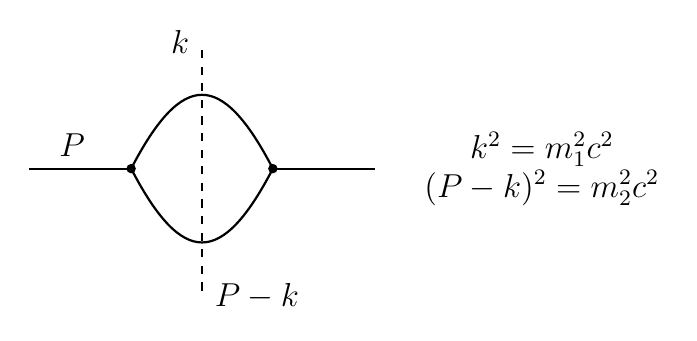
\begin{tikzpicture}[x=1cm,y=1cm,every node/.style={font=\large}]
 \coordinate (L) at (-2.2,0); \coordinate (R) at (2.2,0);
 \coordinate (a) at (-0.9,0); \coordinate (b) at (0.9,0);
 \draw[line width=.8pt] (L)--(a);
 \draw[line width=.8pt] (b)--(R);
 \draw[line width=.8pt] (a) .. controls (-0.25,1.25) and (0.25,1.25) .. (b);
 \draw[line width=.8pt] (a) .. controls (-0.25,-1.25) and (0.25,-1.25) .. (b);
 \fill (a) circle (1.7pt); \fill (b) circle (1.7pt);
 \draw[dashed,line width=1pt] (0,-1.55)--(0,1.55);
 \node at (-1.65,.3) {$P$};
 \node[anchor=south east,fill=white,inner sep=1pt] at (-.12,1.42) {$k$};
 \node[anchor=north west,fill=white,inner sep=1pt] at (.12,-1.42) {$P-k$};
 \node[align=center,right] at (2.7,0) {$k^2=m_1^2c^2$\\$(P-k)^2=m_2^2c^2$};
\end{tikzpicture}

 \caption{二体泡图的幺正性割线。虚线表示把两条内部传播子同时置于正能质量壳；割线积分使用的测度就是相应真实二体 Lorentz 不变相空间。}
 \label{fig:qft-bubble-cut-dp8}
\end{figure}



\begin{derivation}[从\eqnrefs{eq:bubble-imag-phase-space-dp8}到\eqnrefs{eq:two-body-threshold-beta-dp8}]

正文\eqnrefs{eq:bubble-imag-phase-space-dp8} 表明虚部只有在两个内部粒子同时满足正能质量壳和能量守恒时才存在。对等质量情形进入质心系，能量 $\delta$ 函数固定唯一的径向动量 $k_*$；解出这个根并把它写成相对论速度因子，就得到正文\eqnrefs{eq:two-body-threshold-beta-dp8}。

在质心系 $\mathbf P=0$ 且 $m_1=m_2=m$ 时，
\begin{equation*}
 E_1=E_2=E_k=\sqrt{m^2c^4+c^2k^2},
 \qquad
 \sqrt{s}\,c=2E_k.
\end{equation*}
平方后有
\begin{align*}
 sc^2
 &=4m^2c^4+4c^2k_*^2,\\
 k_*^2
 &=\frac{s-4m^2c^2}{4}.
\end{align*}
因此只有 $s\ge4m^2c^2$ 时 $k_*$ 才为实数。再用 $E_{\rm cm}=\sqrt{s}\,c$，
\begin{align*}
 \beta_*(s)
 &=\frac{ck_*}{E_{\rm cm}/2}
 =\frac{2ck_*}{\sqrt{s}\,c}\\
 &=\sqrt{1-\frac{4m^2c^2}{s}},
\end{align*}
即正文\eqnrefs{eq:two-body-threshold-beta-dp8}。为把阈值因子的整体归一化也固定下来，定义正文\eqnrefs{eq:bubble-imag-phase-space-dp8} 中的径向相空间核
\begin{equation*}
 \rho_2(s)
 \equiv
 \int\frac{\dd^3\mathbf k}{(2\pi\hbar)^3}
 \frac{c^2}{4E_k^2}
 \delta\!\left(\sqrt{s}\,c-2E_k\right).
\end{equation*}
利用
\begin{equation*}
 \left.\frac{\dd(2E_k)}{\dd k}\right|_{k_*}
 =\frac{2c^2k_*}{E_*},
 \qquad E_*\equiv E_{k_*}=\frac{\sqrt{s}\,c}{2},
\end{equation*}
径向 $\delta$ 积分严格给出
\begin{align*}
 \rho_2(s)
 &=\frac{4\pi k_*^2}{(2\pi\hbar)^3}
 \frac{c^2}{4E_*^2}
 \frac{E_*}{2c^2k_*}\\
 &=\frac{k_*}{16\pi^2\hbar^3E_*}
 =\frac{\beta_*(s)}{16\pi^2\hbar^3c}.
\end{align*}
因此连续谱在阈值处按确定的线性因子 $\beta_*(s)$ 从零打开。
\end{derivation}

\begin{derivation}[从\eqnrefs{eq:optical-unitarity-r68}到\eqnrefs{eq:perturbative-optical-theorem-dp68}]

正文\eqnrefs{eq:optical-unitarity-r68} 是精确散射算符的幺正性关系。把跃迁算符按耦合阶数展开，并只比较最低出现虚部的二阶项，就能把圈振幅的虚部写成一阶真实跃迁振幅的模平方之和，从而得到正文\eqnrefs{eq:perturbative-optical-theorem-dp68}。

写
\begin{equation*}
 \hat T_S=\hat T^{(1)}+\hat T^{(2)}+\hat T^{(3)}+\cdots .
\end{equation*}
代入
$-\ii(\hat T_S-\hat T_S^\dagger)=\hat T_S^\dagger\hat T_S$，二阶部分为
\begin{equation*}
 -\ii\bigl(\hat T^{(2)}-\hat T^{(2)\dagger}\bigr)
 =\hat T^{(1)\dagger}\hat T^{(1)}.
\end{equation*}
在同一初态 $|i\rangle$ 两侧取矩阵元，并在右端插入在壳中间态完备关系 $\sum_X|X\rangle\langle X|=\mathbb I$，得到
\begin{align*}
 -\ii\left[
 \langle i|\hat T^{(2)}|i\rangle
 -\langle i|\hat T^{(2)}|i\rangle^*
 \right]
 &=\sum_X
 \langle i|\hat T^{(1)\dagger}|X\rangle
 \langle X|\hat T^{(1)}|i\rangle\\
 &=2\operatorname{Im}\langle i|\hat T^{(2)}|i\rangle,
\end{align*}
这就是正文\eqnrefs{eq:perturbative-optical-theorem-dp68}。图形语言中的割线规则只是把右端的在壳中间态完备和翻译成内部传播子的 $\delta_+$ 替换。
\end{derivation}


\subsection{紫外发散、尺度依赖与短距离展开}
圈积分会探测任意大的内部动量，因此中间表达式可能依赖一个人为引入的紫外调节尺度。物理预测不能依赖这个人为选择：需要先把发散写成局域参数的重新定义，再研究当参考尺度改变时这些有限参数怎样随之变化。这种有限参数随重整化尺度的演化就是重整化群。

当计算推广到多圈或局域复合算符时，同一个“短距离效应应由局域结构吸收”的原则仍然成立，只是需要更系统的递归组织。等真正比较两个相近时空点上的算符乘积时，再引入算符乘积展开；热核则只在需要计算一般二次算符的一圈紫外项时出现。
\phantomsection\label{sec:qft-renormalization-rg-dp10}

前面的微扰规则已经把散射振幅写成顶角、传播子和内部动量积分的组合。新的困难出现在圈积分的高动量端：某些积分若一直延伸到任意大的内部动量，会发散，因而“直接代入裸质量和裸耦合再积分”并不是一个完整的计算定义。解决它需要先把发散积分改写成带有临时控制参数的有限表达式，再用实验可定义的质量、耦合和场归一化重新参数化作用量，使最终可观测量不依赖这个临时参数。前一步称为正则化，后一步称为重整化。

重整化以后，同一个物理过程仍可在不同外部能标下被探测，因此有限参数必须随分辨尺度变化而保持可观测量不变；描述这种尺度依赖的微分方程就是重整化群。当实验能量远低于某些重自由度的质量尺度时，这些自由度不能成为真实外态，却仍通过虚过程留下低能效应；有效场论把这些高能效应编码成局域算符及其 Wilson 系数。

圈动量定义为顶角守恒约束后仍未固定的独立内部 Fourier 积分变量；一般内部传播线处于离壳状态。紫外发散说明“裸参数直接等于实验参数”的写法没有把短程贡献与测量条件分开。正则化引入临时数学参数；反项与重整化条件再把这种临时依赖吸收到有限个参数定义中。最终可观测量只依赖物理输入与外部运动学尺度，而不依赖正则化器本身。


共同放大所有独立圈物理四动量，\(\ell_r^\mu\mapsto\Lambda\ell_r^\mu\) 且 \(\Lambda\to\infty\)，即可诊断图的表面紫外次数。四维圈测度贡献四次幂，玻色传播子贡献负二次幂，Dirac 传播子在大动量下贡献负一次幂；若顶角分子还含 \(N_\partial\) 个圈动量因子，则连通图满足
\begin{equation}
 \boxed{
 \omega_{\rm UV}=4L-2I_B-I_F+N_\partial,}
 \label{eq:superficial-degree-general-dp10}
\end{equation}
其中 \(L\) 是独立圈数，\(I_B\) 与 \(I_F\) 分别为内部玻色子线与费米子线数。\(\omega_{\rm UV}<0\) 只说明所有圈动量共同放大时表面收敛，仍须检查发散子图；\(\omega_{\rm UV}\ge0\) 也只是最坏幂次上界，对称性还可以排除相应局域结构。

对四维 \(\varphi^4\) 理论，每个四次顶角提供四个线端。若连通图含 $V$ 个顶角、$I$ 条内部线和 $E$ 条外线，则线端计数与独立圈数满足
\begin{equation}
 \boxed{
 4V=2I+E,
 \qquad
 L=I-V+1.}
 \label{eq:phi4-topology-r68}
\end{equation}
把这两条纯拓扑关系代入\eqnrefs{eq:superficial-degree-general-dp10}，便得到
\begin{equation}
 \boxed{\omega_{\varphi^4}=4-E,}
 \label{eq:phi4-superficial-degree-dp10}
\end{equation}
所以除真空图外，只有二点与四点函数需要原理论已有的质量、场强和四次耦合局域结构作为反项。QED 的每个最小耦合顶角连接一个光子腿和两个费米子腿。相应的光子线端、费米子线端和独立圈数同时满足
\begin{equation}
 \boxed{
 V=2I_\gamma+E_\gamma,
 \qquad
 2V=2I_\psi+E_\psi,
 \qquad
 L=I_\gamma+I_\psi-V+1.}
 \label{eq:qed-topology-r68}
\end{equation}
把这些拓扑恒等式代入 $\omega=4L-2I_\gamma-I_\psi$，即可消去内部线数并得到
\begin{equation}
 \boxed{
 \omega_{\rm QED}=4-E_\gamma-\frac32E_\psi.}
 \label{eq:qed-superficial-degree-dp10}
\end{equation}
例如光子二点函数表面计数给二次发散，但 Ward 恒等式要求 \(q_\mu\Pi^{\mu\nu}=0\)，把允许张量限制到横向结构，实际只剩对数发散。幂次计数决定潜在紫外阶数，规范对称性再决定哪些局域项真正允许出现。

发散积分必须先被数学地定义。维数正则化取
\begin{equation*}
 d=4-2\epsilon,
 \qquad \epsilon>0,
\end{equation*}
并引入具有\emph{物理四动量量纲}的尺度 \(\mu_{\rm DR}\)。四维无量纲耦合的一般圈积分写成
\begin{equation}
 \boxed{
 \mu_{\rm DR}^{2\epsilon}
 \int\frac{\dd^d \ell}{(2\pi)^d}(\cdots),}
 \label{eq:dim-reg-measure-general-dp10}
\end{equation}
其中 $\ell^\mu$ 始终是物理四动量。若改用逆长度变量 $\kappa^\mu=\ell^\mu/\hbar$，则测度提供 $\hbar^{-d}$，两个二次传播子分母提供 $\hbar^4$，而维数正则化尺度 $\mu_\kappa^{2\epsilon}=(\mu_{\rm DR}/\hbar)^{2\epsilon}$ 再提供 $\hbar^{-2\epsilon}$。因为 $d=4-2\epsilon$，总幂次
\[
 -d+4-2\epsilon=0
\]
恰好为零，因此物理动量形式中的显式 $\hbar$ 由变量换元严格抵消。典型积分在 $\epsilon\to0$ 时产生局域极点与外部尺度对数；前者由反项吸收，后者保留为可测尺度依赖。

有外部四动量时，一圈分子通常还含 $\ell^\mu$、$\ell^\mu\ell^\nu$ 等张量。Lorentz 协变性保证它们只能展开在 $\eta^{\mu\nu}$ 与外部四动量张量基上，因此张量积分可以先约化为少数标量母积分；这一步称为 Passarino--Veltman 约化。沿用\eqnrefs{eq:reduced-loop-measure-si-r10} 的物理四动量测度，对任意具有动量量纲的质量参数 $M_i$ 定义
\begin{equation}
\boxed{
\begin{aligned}
 A_0(M^2)
 &\equiv \frac{16\pi^2}{\ii}\int_\ell^{(d)}
 \frac{1}{\ell^2-M^2+\ii0},\\
 B_0(p^2;M_1^2,M_2^2)
 &\equiv \frac{16\pi^2}{\ii}\int_\ell^{(d)}
 \frac{1}{(\ell^2-M_1^2+\ii0)[(\ell+p)^2-M_2^2+\ii0]},\\
 C_0(p_1^2,p_2^2,(p_1+p_2)^2;M_1^2,M_2^2,M_3^2)
 &\equiv \frac{16\pi^2}{\ii}\int_\ell^{(d)}
 \frac{1}{D_1D_2D_3},
\end{aligned}}
\label{eq:pv-scalar-masters-dp90}
\end{equation}
其中
\[
D_1=\ell^2-M_1^2+\ii0,\quad
D_2=(\ell+p_1)^2-M_2^2+\ii0,\quad
D_3=(\ell+p_1+p_2)^2-M_3^2+\ii0.
\]
按这一定义，$A_0$、$B_0$、$C_0$ 的动量量纲依次为 $2,0,-2$。例如秩二三点积分不需要引入新的非标量函数作为物理输入，因为必可写成
\begin{equation}
\frac{16\pi^2}{\ii}\int_\ell^{(d)}\frac{\ell^\mu\ell^\nu}{D_1D_2D_3}
=C_{00}\eta^{\mu\nu}+\sum_{i,j=1}^{2}C_{ij}p_i^\mu p_j^\nu .
\label{eq:pv-rank2-decomposition-dp90}
\end{equation}
分别用 $\eta_{\mu\nu}$、$p_{1\mu}p_{1\nu}$、$p_{1\mu}p_{2\nu}$、$p_{2\mu}p_{2\nu}$ 收缩即可得到 $C_{00},C_{ij}$ 的线性方程；再利用 $2\ell\!\cdot p_i$ 与相邻传播子分母之差，把右端化为\eqnrefs{eq:pv-scalar-masters-dp90}。因此 QED、QCD 与标准模型的一圈张量约化都归结为同一件事：先在 Lorentz 张量基上展开，再用传播子恒等式把张量积分精确消元为标量主积分。

重整化把同一裸作用量精确拆成“用有限参数写成的原型拉氏量 + 局域反项”。以实标量场为例，写成
\begin{equation*}
 \varphi_B=Z_\varphi^{1/2}\varphi_R,
 \qquad
 m_B^2=m_R^2+\delta m^2+\cdots,
 \qquad
 g_{4,B}=\mu_{\rm DR}^{2\epsilon}(g_4+\delta g_4),
\end{equation*}
即可得到
\begin{equation*}
 \Lag_B=\Lag_{\rm R}+\Lag_{\rm ct}.
\end{equation*}
反项系数由重整化条件以及裸理论对临时正则化参数的独立性确定。

\begin{note}[常用重整化方案]
壳上方案以传播子物理极点、留数和指定运动学点的电荷作为输入；最小减除只减去 \(1/\epsilon\) 极点；\(\overline{\rm MS}\) 方案同时减去 \(1/\epsilon-\gamma_E+\ln4\pi\)。有限阶计算会保留方案依赖，但同一可观测量在相同完整微扰阶上的方案差异属于更高阶截断误差。
\end{note}


\begin{exbox}[$\varphi^4$ 理论的三类重整化]
单靠“圈积分发散”还看不出应该重定义哪个参数。最清楚的办法是分别看二点函数与四点函数。

一圈二点 1PI 图只有一个四次顶角。两条外腿占用顶角的两个场，剩余两个场彼此收缩成蝌蚪圈，因此
\begin{equation}
 \boxed{
 -\ii\Sigma_{\rm tad}^{(1)}
 =\frac{-\ii g_4}{2}
 \mu_{\rm DR}^{2\epsilon}
 \int\frac{\dd^d \ell}{(2\pi)^d}
 \frac{\ii}{\ell^2-m_R^2c^2+\ii0^+}.}
 \label{eq:phi4-tadpole-selfenergy-dp52}
\end{equation}
$1/2$ 是同一顶角上两条内部腿互换的对称性因子。这个积分不含外部四动量 $p$，所以它只能平移传播子极点的位置，而不能改变极点附近对 $p^2$ 的斜率。于是四维 $\varphi^4$ 理论在一圈阶满足
\begin{equation}
 \boxed{
 \delta m^2=O(g_4),
 \qquad
 Z_\varphi=1+O(g_4^2).}
 \label{eq:phi4-one-loop-mass-vs-Z-dp52}
\end{equation}
也就是说，质量反项在一圈就需要，场强反项要到二圈才第一次被二点函数要求。

四点函数的情况不同。$g_4^2$ 阶出现 $s,t,u$ 三个泡图，每个都依赖外部不变量，并具有同一个局域对数紫外极点。它们不能由质量反项消去，而必须重定义四次耦合。于是“哪一种反项出现”并不是预先背下来的规则，而是由 1PI 函数的外腿数和外部动量结构决定：二点函数的常数部分固定质量，二点函数的 $p^2$ 斜率固定场强，四点函数在指定运动学点的值固定耦合。

把重整化后二点函数写成
\begin{equation}
 \widetilde G_R(p)
 =\frac{\ii}
 {p^2-m_R^2c^2-\Sigma_R(p^2)+\ii0^+},
 \label{eq:phi4-ren-propagator-dp52}
\end{equation}
壳上方案直接把“物理质量”和“单位极点留数”翻译成
\begin{equation}
 \boxed{
 \Sigma_R(m_R^2c^2)=0,
 \qquad
 \left.\frac{\dd\Sigma_R}{\dd p^2}\right|_{p^2=m_R^2c^2}=0.}
 \label{eq:phi4-onshell-ren-conditions-dp52}
\end{equation}
第一式固定极点位置，第二式固定极点斜率。$\overline{\rm MS}$ 不直接采用这两个物理条件，而只减去维数正则化极点；两种方案得到的中间参数不同，但把参数都换成同一组实验输入后，可观测量只在被截掉的更高微扰阶上不同。


\medskip

\eqnrefs{eq:phi4-tadpole-selfenergy-dp52} 是 $\varphi^4$ 二点 1PI 函数的一圈蝌蚪贡献。由于积分与外部四动量无关，它在这一阶只移动传播子的极点位置，而不产生随 $p^2$ 变化的紫外斜率项。顶角收缩计数给出 $1/2$ 对称因子；维数正规化把紫外极点显式分离，质量与场强反项分别控制逆传播子的常数项和 $p^2$ 斜率。把重整化逆传播子在物理极点附近展开并固定极点位置与留数，便得到\eqnrefs{eq:phi4-onshell-ren-conditions-dp52}。



从相互作用
\begin{equation*}
 \Lag_{\rm int}
 =-\frac{g_4}{4!\,\hbar c}\varphi^4
\end{equation*}
的一阶 Dyson 插入开始。为形成二点 1PI 函数，两个外部场必须分别与顶角上的两个场收缩；选择有序外腿的方式数为
\begin{equation*}
 4\times3=12.
\end{equation*}
剩余两个顶角场彼此收缩只有一种方式。作用量中的 $1/4!=1/24$ 因而留下
\begin{equation*}
 \frac{12}{24}=\frac12,
\end{equation*}
这就是\eqnrefs{eq:phi4-tadpole-selfenergy-dp52} 的对称性因子。内部线从顶角出发又回到同一顶角，没有任何外部四动量流经圈，因此积分只依赖 $m_R$ 与正则化尺度，而不依赖 $p$。

令
\begin{equation*}
 T(m_R^2)
 \equiv
 \mu_{\rm DR}^{2\epsilon}
 \int\frac{\dd^d \ell}{(2\pi)^d}
 \frac{\ii}{\ell^2-m_R^2c^2+\ii0^+}.
\end{equation*}
用 Schwinger 参数
\begin{equation*}
 \frac{\ii}{\ell^2-m_R^2c^2+\ii0^+}
 =\int_0^\infty\dd\tau\,
 \ee^{\ii\tau(\ell^2-m_R^2c^2+\ii0^+)},
\end{equation*}
把动量积分化成 $d$ 维高斯积分，再对 $\tau$ 积分，得到解析延拓形式
\begin{equation*}
 T(m_R^2)
 =\frac{\mu_{\rm DR}^{2\epsilon}}
 {(4\pi)^{d/2}}
 \Gamma\!\left(1-\frac d2\right)
 (m_R^2c^2)^{d/2-1}.
\end{equation*}
取 $d=4-2\epsilon$，并展开
\begin{align*}
 \Gamma(-1+\epsilon)
 &=-\frac1\epsilon+\gamma_E-1+O(\epsilon),\\
 (4\pi)^\epsilon
 \left(\frac{\mu_{\rm DR}^2}{m_R^2c^2}\right)^\epsilon
 &=1+\epsilon
 \left[
 \ln4\pi+\ln\frac{\mu_{\rm DR}^2}{m_R^2c^2}
 \right]+O(\epsilon^2),
\end{align*}
所以
\begin{equation*}
 T(m_R^2)
 =-\frac{m_R^2c^2}{16\pi^2}
 \left[
 \frac1{\bar\epsilon}
 +1-\ln\frac{m_R^2c^2}{\mu_{\rm DR}^2}
 \right]
 +O(\epsilon),
\end{equation*}
其中 $1/\bar\epsilon=1/\epsilon-\gamma_E+\ln4\pi$。这个结果的关键结构是“局域、与 $p$ 无关、正比于 $m_R^2c^2$”；其有限常数部分会随减除方案改变，而这三个结构不会改变。

把裸二次部分写成重整化场与反项：
\begin{equation*}
 \frac12 Z_\varphi(\partial\varphi_R)^2
 -\frac12 Z_\varphi m_B^2c^2\frac{\varphi_R^2}{\hbar^2}
 =\frac12(\partial\varphi_R)^2
 -\frac12m_R^2c^2\frac{\varphi_R^2}{\hbar^2}
 +\Lag_{\rm ct}^{(2)}.
\end{equation*}
在动量空间，二点反项只能产生
\begin{equation*}
 \Sigma_{\rm ct}(p^2)
 =A_{\rm ct}+B_{\rm ct}(p^2-m_R^2c^2),
\end{equation*}
其中常数 $A_{\rm ct}$ 由质量反项控制，斜率 $B_{\rm ct}$ 由 $\delta Z_\varphi$ 控制。由于一圈蝌蚪满足
\begin{equation*}
 \frac{\dd\Sigma_{\rm tad}^{(1)}}{\dd p^2}=0,
\end{equation*}
一圈阶没有任何紫外斜率需要 $\delta Z_\varphi$ 抵消，因此
\begin{equation*}
 \delta Z_\varphi^{(1)}=0,
 \qquad
 Z_\varphi=1+O(g_4^2),
\end{equation*}
而常数紫外极点必须由 $\delta m^2=O(g_4)$ 吸收。这得到\eqnrefs{eq:phi4-one-loop-mass-vs-Z-dp52}。

最后检查壳上条件。精确重整化传播子定义为
\begin{equation*}
 \widetilde G_R(p)
 =\frac{\ii}
 {p^2-m_R^2c^2-\Sigma_R(p^2)+\ii0^+}.
\end{equation*}
要求物理极点仍位于 $p^2=m_R^2c^2$，分母在该点必须为零，因此
\begin{equation*}
 \Sigma_R(m_R^2c^2)=0.
\end{equation*}
在极点附近令 $p^2=m_R^2c^2+\delta$，Taylor 展开
\begin{align*}
 p^2-m_R^2c^2-\Sigma_R(p^2)
 &=\delta
 -\Sigma_R(m_R^2c^2)
 -\delta\,\Sigma_R'(m_R^2c^2)
 +O(\delta^2),\\
 &=\delta\,[1-\Sigma_R'(m_R^2c^2)]
 +O(\delta^2).
\end{align*}
若把重整化场定义成极点留数为 1，就必须再要求
\begin{equation*}
 \Sigma_R'(m_R^2c^2)=0.
\end{equation*}
这正是\eqnrefs{eq:phi4-onshell-ren-conditions-dp52}。因此质量反项与场强反项分别控制“极点位置”和“极点留数”；它们不是两个形式相似但物理意义不明的常数。
\end{exbox}

四维 \(\varphi^4\) 理论把“正则化—反项—尺度流”三步直接连在一起。一圈四点函数的三个通道都归结为同一个标量泡图。以 \(s\) 通道为例，先把需要计算的标量泡图明确写成
\begin{equation}
 \boxed{
 I(s)=\mu_{\rm DR}^{2\epsilon}
 \int\frac{\dd^d \ell}{(2\pi)^d}
 \frac{\ii}
 {\bigl(\ell^2-m_R^2c^2+\ii0^+\bigr)
  \bigl((\ell+p)^2-m_R^2c^2+\ii0^+\bigr)},
 \qquad p^2=s.}
 \label{eq:phi4-bubble-integral-r68}
\end{equation}
对\eqnrefs{eq:phi4-bubble-integral-r68} 做 Feynman 参数化和维数正则化后得到
\begin{equation}
 \boxed{
 I(s)
 =-\frac1{16\pi^2}
 \left[
 \frac1{\bar\epsilon}
 -\int_0^1\dd x\,
 \ln\frac{m_R^2c^2-x(1-x)s-\ii0^+}{\mu_{\rm DR}^2}
 \right]
 +\order(\epsilon),}
 \label{eq:phi4-bubble-result-dp10}
\end{equation}
其中 \(1/\bar\epsilon\equiv1/\epsilon-\gamma_E+\ln4\pi\)。三个通道具有相同的局域紫外极点，因此在 $d=4-2\epsilon$ 中，$\overline{\rm MS}$ 的一圈裸耦合可以写为
\begin{equation}
 \boxed{
 g_{4,B}
 =\mu^{2\epsilon}
 \left[
 g_4(\mu)
 +\frac{3}{32\pi^2}\frac{g_4^2(\mu)}{\bar\epsilon}
 +\order(g_4^3)
 \right].}
 \label{eq:phi4-bare-coupling-r68}
\end{equation}
裸参数不能依赖人为引入的减除尺度。对\eqnrefs{eq:phi4-bare-coupling-r68} 在固定 $g_{4,B}$ 下求尺度导数，得到
\begin{equation}
 \boxed{
 \beta_{g_4}(g_4)
 \equiv
 \mu\frac{\dd g_4}{\dd\mu}\Big|_{g_{4,B}}
 =\frac{3g_4^2}{16\pi^2}+\order(g_4^3).}
 \label{eq:phi4-beta-one-loop-dp10}
\end{equation}
一圈积分解为
\begin{equation}
 \boxed{
 \frac1{g_4(\mu)}
 =\frac1{g_4(\mu_0)}
 -\frac{3}{16\pi^2}\ln\frac\mu{\mu_0}.}
 \label{eq:phi4-running-one-loop-dp10}
\end{equation}

\begin{exbox}[一圈运行的数值尺度]
设某个参考尺度 $\mu_0$ 上测得 $g_4(\mu_0)=1$。先把分辨尺度提高三个数量级，考察一个仍然温和的尺度比
\begin{equation*}
 \frac\mu{\mu_0}=10^3,
 \qquad
 \ln\frac\mu{\mu_0}=6.9078.
\end{equation*}
一圈解给
\begin{align*}
 \frac1{g_4(\mu)}
 &=1-\frac{3}{16\pi^2}(6.9078)\\
 &\simeq0.8688,
\end{align*}
所以
\begin{equation*}
 g_4(10^3\mu_0)\simeq1.151.
\end{equation*}
耦合本身只增加约 $15\%$，但固定阶展开中真正控制大对数的是
\begin{equation*}
 \epsilon_{\log}
 \equiv\frac{g_4}{16\pi^2}\left|\ln\frac\mu{\mu_0}\right|
 \simeq4.37\times10^{-2},
\end{equation*}
仍明显小于 1，因此一圈结果在这个例子里仍是受控的。

继续把一圈解的分母外推到零，可得到形式上的 Landau 极点
\begin{equation*}
 \frac{\mu_L}{\mu_0}
 =\exp\!\left(\frac{16\pi^2}{3g_4(\mu_0)}\right)
 \simeq7.3\times10^{22}
 \qquad[g_4(\mu_0)=1].
\end{equation*}
这个巨大数字不应被误读成“一圈理论精确预言了一个真实新粒子能标”。它只说明正的一圈 $\beta$ 函数会让耦合随紫外尺度增大，并且若坚持把同一低阶方程外推足够远，最终一定离开微扰控制区。重整化群的价值正是把这种尺度积累显式量化出来。
\end{exbox}

普通固定阶一圈截断要求 \(g_4/(16\pi^2)\ll1\)；跨越很大的尺度比时还需 \(|g_4\ln(\mu/\mu_0)|/(16\pi^2)\ll1\)，否则应使用重整化群方程重求和大对数，而不是继续展开\eqnrefs{eq:phi4-bubble-result-dp10} 的有限阶对数。

任意重整化 $n$ 点函数的尺度依赖应从整个重整化参数空间一次建立。若裸场与重整化场满足 $\varphi_B=Z_\varphi^{1/2}\varphi_R$，同一组外点的裸与重整化关联函数满足
\begin{equation}
 \boxed{
 G_B^{(n)}=Z_\varphi^{n/2}G_R^{(n)}.}
 \label{eq:bare-ren-green-relation-r68}
\end{equation}
设理论含一组无量纲耦合 $\{g_a(\mu)\}$ 和一组质量参数 $\{m_b(\mu)\}$。耦合和质量对尺度的对数导数分别描述参数怎样随分辨尺度流动；场归一化因子 $Z_\varphi$ 的尺度导数则描述量子涨落使场偏离经典工程尺度律的程度。后一个量通常称为场的\emph{反常维数}；“反常”在这里只表示额外的量子尺度修正，并不表示理论发生了量子对称性反常。具体定义为
\begin{equation}
\boxed{
 \beta_{g_a}\equiv\mu\frac{\dd g_a}{\dd\mu}\bigg|_{\rm bare},
 \qquad
 \beta_{m_b}\equiv\mu\frac{\dd m_b}{\dd\mu}\bigg|_{\rm bare},
 \qquad
 \gamma_\varphi\equiv\frac12\mu\frac{\dd\ln Z_\varphi}{\dd\mu}\bigg|_{\rm bare}.}
\label{eq:rg-general-flow-definitions-dp74}
\end{equation}
固定所有裸参数时，$G_B^{(n)}$ 不依赖人为减除尺度，因此得到一般尺度方程
\begin{equation}
 \boxed{
 \left[
 \mu\frac{\partial}{\partial\mu}
 +\sum_a\beta_{g_a}\frac{\partial}{\partial g_a}
 +\sum_b\beta_{m_b}\frac{\partial}{\partial m_b}
 +n\gamma_\varphi
 \right]G_R^{(n)}=0.}
 \label{eq:callan-symanzik-general-dp10}
\end{equation}
这条方程描述重整化参数空间上的全尺度流。若只保留一个耦合 $g_{\rm R}$ 和一个质量 $m$，上式退化为
\[
 \left(
 \mu\partial_\mu+\beta_{g_{\rm R}}\partial_{g_{\rm R}}
 +\beta_m\partial_m+n\gamma_\varphi
 \right)G_R^{(n)}=0,
\]
这正是前面 $\varphi^4$ 一圈运行的参数特例。

局域复合算符具有另一种尺度结构。多个具有相同守恒量子数的算符在改变量子分辨尺度时可以彼此混合，因此它们的尺度修正不再由一个数描述，而由算符空间中的矩阵描述。这个矩阵就是复合算符的反常维数矩阵。若一组算符满足
\begin{equation}
\boxed{
 \mathcal O_i^B=Z_{ij}^{(\mathcal O)}\mathcal O_j^R,
 \qquad
 \gamma^{(\mathcal O)}
 =(Z^{(\mathcal O)})^{-1}\mu\frac{\dd Z^{(\mathcal O)}}{\dd\mu},}
\label{eq:operator-mixing-general-dp74}
\end{equation}
那么 $\gamma^{(\mathcal O)}$ 从一开始就是算符空间上的线性算符；其非对角元表示尺度流把一个基算符混入另一个基算符。只有在该空间恰为一维时，它才退化成单个反常维数。

\phantomsection\label{sec:qft-eft-unitarity-dp10}
重整化控制给定理论内部的紫外敏感性，却不要求低能实验显式解析所有高能自由度。若某些自由度的特征能量远高于实验能量，它们不能作为真实外态产生，但仍会通过虚过程改变低能振幅。

有效场论（effective field theory，EFT）只保留当前分辨率能够直接激发的轻自由度，并把重自由度的虚效应编码为由轻场构成的局域高维算符。若实验特征动量远小于重尺度，局域展开就按“实验动量/重尺度”的幂次有序；算符维数越高，通常受到越高次幂的抑制。EFT 的适用范围因此首先由这一无量纲展开参数控制，并还需满足散射矩阵幺正性等一致性界限。

采用 \(x^0=ct\)，定义几何拉氏量密度 \(\widehat\Lag=\Lag/(\hbar c)\)。同一个重尺度可等价写成逆长度、物理动量或能量：
\begin{equation}
 \boxed{
 \Lambda_*\ [\mathrm{m^{-1}}],
 \qquad
 p_*\equiv\hbar\Lambda_*,
 \qquad
 \Lambda_E\equiv cp_*=\hbar c\Lambda_*.}
 \label{eq:qft-eft-three-scales-dp42}
\end{equation}
若局域算符 \(\widehat{\mathcal O}_i\) 的逆长度工程维数为 \(\Delta_i>4\)，一般低能有效拉氏量为
\begin{equation}
 \boxed{
 \widehat\Lag_{\rm EFT}
 =\widehat\Lag_{\Delta\le4}
 +\sum_{\Delta_i>4}
 \frac{c_i}{\Lambda_*^{\Delta_i-4}}
 \widehat{\mathcal O}_i,}
 \label{eq:eft-operator-suppression-dp10}
\end{equation}
其中 \(c_i\) 无量纲。它们记录被消去高能自由度的短距离信息，而低能算符 \(\widehat{\mathcal O}_i\) 描述仍可分辨的自由度；乘在局域有效算符前的这些短距离系数称为\emph{Wilson 系数}。

Wilson 系数不能仅凭低能理论自身决定：应选择一组低能外态或 Green 函数，在包含重自由度的完整理论与有效理论中分别计算，并要求两种描述在共同适用的低能区域逐阶给出相同结果。用这种“比较同一低能物理并据此固定 Wilson 系数”的步骤称为\emph{匹配}（matching）。匹配解决的是高能信息怎样进入低能系数，而随后随重整化尺度改变这些系数则是另一个独立的重整化群问题。特征外部物理动量为 \(Q\) 时，维数 \(\Delta_i\) 的算符典型贡献按
\begin{equation}
 \boxed{
 \epsilon_{\rm EFT}^{(i)}
 \sim
 \left(\frac{Q}{p_*}\right)^{\Delta_i-4}
 \ll1}
 \label{eq:eft-power-counting-dp10}
\end{equation}
排序。若 \(Q\sim p_*\)，局域高维展开失去层级，必须恢复被消去的高能自由度或改用非局域描述。

有效场论把未解析的高能自由度编码为高维局域算符，并以 \(Q/p_*\) 排序；Feshbach--Schur、Schrieffer--Wolff 与 Green 张量投影则利用谱隙或预解式消去远失谐或连续自由度，控制参数通常是耦合与能隙之比以及预解式的能量依赖。二者都只保留给定能窗内可分辨的自由度，但展开参数不同。


有效场论截断还必须满足散射矩阵幺正性。对无自旋、单通道弹性 \(2\to2\) 散射，在质心系定义
\begin{equation}
 \boxed{
 \mathcal M(s,\theta)
 =16\pi\sum_{\ell=0}^{\infty}(2\ell+1)
 a_\ell(s)P_\ell(\cos\theta).}
 \label{eq:partial-wave-expansion-dp10}
\end{equation}
单弹性通道中 \(S_\ell=1+2\ii a_\ell\)，由 \(|S_\ell|=1\) 得到 Argand 圆，因此
\begin{equation}
 \boxed{
 |a_\ell|\le1,
 \qquad
 |\Re a_\ell|\le\frac12.}
 \label{eq:partial-wave-unitarity-bound-dp10}
\end{equation}
存在非弹性通道时允许区域收缩到圆盘内部。若树级有效场论振幅已经增长到 \(|\Re a_\ell|\gtrsim1/2\)，失效的是固定阶低能截断；此时必须加入圈修正、重求和或新的高能自由度，而不能把精确理论解释为“不幺正”。

幂次计数判断潜在紫外行为；正则化定义发散积分；重整化用有限输入定义参数；重整化群组织减除尺度变化；有效场论按 \(Q/p_*\) 排列未解析高能结构；分波幺正性给出振幅的非微扰边界。QED、QCD 与电弱理论的规范群和场内容不同，但共享这套紫外组织原则。


这些结构可与 \cite{PeskinSchroeder1995,Schwartz2014QFT} 对照；全部尺度均按物理四动量与 SI 约定解释，并显式保留 \(c\) 与 \(\hbar\)。

% 多圈重整化、复合算符混合、算符乘积展开与有限温度边界条件
单圈原始发散图通常只有一个整体紫外发散，需要相应的局域反项吸收。进入多圈以后，同一图内部还会出现嵌套或重叠的发散真子图。若等整张图积分完成后再一次性减去极点，子图发散会被带入更高阶图中，无法由局域参数重定义逐阶吸收。局域性因此要求一种递归减除：先对所有真子图完成重整化，再处理缩约图剩余的整体发散。

对一张单粒子不可约图 $\Gamma$，记维数正则化后的裸振幅为 $I_\Gamma$。令线性算符 $K$ 只抽取所选减除方案中的局域紫外发散部分；例如在修正的最小减除方案（$\overline{\rm MS}$）中，$K$ 抽取所有 $1/\bar\epsilon^n$ 极点。对没有发散真子图的原始发散图，反项定义为
\begin{equation*}
 C(\Gamma)=-K I_\Gamma.
\end{equation*}
存在发散真子图时，先把所有真子图的局域反项插回原图，定义不完全 $R$ 运算
\begin{equation}
 \boxed{
 \bar R I_\Gamma
 =I_\Gamma
 +\sum_{\{\gamma_i\}}
 \left[\prod_i C(\gamma_i)\right]
 I_{\Gamma/\{\gamma_i\}}.}
 \label{eq:rbar-operation-dp68}
\end{equation}
其中求和遍历两两不重叠的紫外发散真子图集合，$\Gamma/\{\gamma_i\}$ 表示把每个 $\gamma_i$ 缩成一个局域顶角。完整 $R$ 运算由
\begin{equation}
 \boxed{
 C(\Gamma)=-K\bar RI_\Gamma,
 \qquad
 RI_\Gamma=(1-K)\bar RI_\Gamma}
 \label{eq:r-operation-dp11}
\end{equation}
给出。第一式只抽取已经消除子图发散后剩余的整体局域极点；第二式留下有限的重整化图。

嵌套与重叠子图可以用 Zimmermann 森林公式统一组织。森林 $F$ 是一组彼此不重叠或互相包含的发散真子图，$T_\gamma$ 表示对子图 $\gamma$ 作局域减除。Zimmermann 定理把递归过程写成
\begin{equation}
 \boxed{
 RI_\Gamma
 =\sum_{F\in\operatorname{Forests}(\Gamma)}
 \left(\prod_{\gamma\in F}(-T_\gamma)\right)I_\Gamma.}
 \label{eq:zimmermann-forest-dp11}
\end{equation}
空森林给出原图；含一个子图的森林给一次减除；嵌套森林自动按从内到外的顺序作用。定理的关键假设是紫外发散部分在外动量和轻质量上可作局域 Taylor 展开，因此 $T_\gamma$ 抽取的是有限阶局域多项式。这一局域性正是多圈反项仍能写回原拉格朗日量允许算符的原因。

重整化局域算符还需要处理重合点奇异性，因此场与耦合的重整化之后必须进一步引入复合算符混合。

分离时空点的 Green 函数完成重整化后，局域复合算符仍会产生额外的重合点奇异性。若一组算符 $\mathcal O_i$ 具有相同守恒量子数，重整化一般不是逐个乘一个常数，而是矩阵混合：
\begin{equation}
 \boxed{\mathcal O_{i,B}=Z_{ij}^{\mathcal O}\mathcal O_{j,R}.}
 \label{eq:composite-operator-mixing-dp11}
\end{equation}
定义反常维数矩阵
\begin{equation*}
 \gamma^{\mathcal O}
 \equiv (Z^{\mathcal O})^{-1}\mu\frac{\dd Z^{\mathcal O}}{\dd\mu},
\end{equation*}
即可得到
\begin{equation*}
 \mu\frac{\dd}{\dd\mu}\mathcal O_{i,R}
 =-\gamma_{ij}^{\mathcal O}\mathcal O_{j,R}.
\end{equation*}
若有效拉格朗日量含 $C_i(\mu)\mathcal O_i(\mu)$，物理作用量不能依赖任意重整化尺度，因此 Wilson 系数沿相反方向演化：
\begin{equation}
 \boxed{
 \mu\frac{\dd C_i}{\dd\mu}
 =C_j\gamma_{ji}^{\mathcal O}.}
 \label{eq:wilson-rg-dp11}
\end{equation}
多个局域算符之间的尺度演化都具有这一矩阵结构；具体物理系统只改变算符基与反常维数矩阵。

复合算符的尺度演化确定以后，短距离乘积可以继续按同一局域算符基展开，从而把短程系数与长程矩阵元分离。

当两个重整化局域算符的类空间隔 $x$ 远小于强子、介质或外态的长程尺度时，局域性允许把短距离乘积按局域算符基作渐近展开。算符乘积展开（OPE）的结构为
\begin{equation}
 \boxed{
 \mathcal O_A(x)\mathcal O_B(0)
 \sim\sum_i C_{AB}^{\ \ i}(x,\mu)\mathcal O_i(0,\mu),
 \qquad x\to0.}
 \label{eq:ope-general-dp11}
\end{equation}
Wilson 系数 $C_{AB}^{\ i}$ 编码距离尺度 $|x|$ 附近的短程物理，在硬尺度足够高时可用微扰理论计算。外态矩阵元 $\langle H|\mathcal O_i|H\rangle$ 则承载长程动力学。

OPE 按算符维数与对称性排序。截断误差由下一批被省略算符相对于保留项的幂次决定，而不能只看某一个 Wilson 系数是否数值很小。

\eqnrefs{eq:ope-general-dp11} 的两边必须具有相同的重整化尺度依赖。复合算符的混合因此强制 Wilson 系数满足耦合的矩阵重整化群方程；选择 $\mu$ 接近短距离硬尺度可以把大对数从固定阶系数中转移到尺度演化中。具体的短程--长程分离问题只需把相应算符基和外态代入这一一般结构。

自由场给出一个最直接的检查。Wick 定理给
\begin{equation*}
 \varphi(x)\varphi(0)
 =\mathcal C(x)+:\!\varphi(x)\varphi(0)\!:.
\end{equation*}
对正规序部分在 $x=0$ 附近作 Taylor 展开，
\begin{equation*}
 :\!\varphi(x)\varphi(0)\!:
 =:\!\varphi^2(0)\!:
 +x^\mu:\!(\partial_\mu\varphi)\varphi\!:(0)+\cdots.
\end{equation*}
单位算符的 Wilson 系数就是短距离奇异的传播子 $\mathcal C(x)$，而 $:\!\varphi^2\!:$ 等局域算符承载较软的场信息。相互作用理论中的 OPE 保留这一职责分离，但系数和算符都必须经过重整化并允许混合。

零温连续频率积分在热平衡态中还会因虚时间边界条件离散化。热密度算符由
\begin{equation*}
 \hat\rho_{\beta_T}=\frac{\ee^{-\beta_T\hat H}}{Z(\beta_T)},
 \qquad Z(\beta_T)=\Tr \ee^{-\beta_T\hat H},
 \qquad \beta_T=(k_BT)^{-1}
\end{equation*}
定义。把实时间解析延拓到虚时间 $t=-\ii\tau$ 后，迹的循环性给出 Kubo--Martin--Schwinger 边界条件：玻色场在 $\tau\to\tau+\beta_T\hbar$ 下周期，费米场反周期，
\begin{align}
 \phi(\tau+\beta_T\hbar)&=+\phi(\tau),\\
 \psi(\tau+\beta_T\hbar)&=-\psi(\tau).
 \label{eq:matsubara-boundary-dp11}
\end{align}
因此虚时 Fourier 模式只能取离散的 Matsubara 频率
\begin{equation}
 \boxed{
 \begin{aligned}
 \omega_n^{(B)}&=\frac{2\pi n}{\beta_T\hbar},\\
 \omega_n^{(F)}&=\frac{(2n+1)\pi}{\beta_T\hbar}.
 \end{aligned}}
 \label{eq:matsubara-frequencies-dp11}
\end{equation}
零温圈积分中的连续频率测度相应替换为
\begin{equation}
 \boxed{
 \int\frac{\dd\omega}{2\pi}
 \longrightarrow
 \frac1{\beta_T\hbar}\sum_n.}
 \label{eq:matsubara-loop-replacement-dp11}
\end{equation}
例如自由玻色子的虚时传播子分母为 $(\omega_n^{(B)})^2+\omega_{\mathbf k}^2$。完成频率求和后出现 Bose--Einstein 分布；统计因子由热边界条件与传播子谱极点共同决定。



多圈 $R$ 运算要求紫外反项保持局域；复合算符重整化把重合点奇异性组织成混合矩阵；算符乘积展开再把短距离奇异性编码进 Wilson 系数。三者描述的是同一局域量子场论在不同尺度组织方式下的同一个紫外结构。


泛函行列式的固有时表示把一圈紫外问题转化为短固有时的局域渐近展开。对欧氏正谱二次算符 \(\Delta\)，先选取逆长度减除尺度 \(\mu_\kappa\,[\mathrm{m^{-1}}]\)。谱定理把标量恒等式 \(\ln(\lambda/\mu_\kappa^2)\) 提升为
\begin{equation}
 \boxed{
 \Tr\ln\frac{\Delta}{\mu_\kappa^2}
 =-\int_0^\infty\frac{\dd s}{s}
 \Tr\!\left(\ee^{-s\Delta}-\ee^{-s\mu_\kappa^2}\right).}
 \label{eq:proper-time-functional-dp11}
\end{equation}
因为 \(\Delta\) 的本征值具有 \(\mathrm{m^{-2}}\) 量纲，固有时 \(s\) 具有 \(\mathrm{m^2}\) 量纲；大本征值对应 \(s\to0^+\)，所以紫外发散完全由热核的短时系数决定。若改用物理动量尺度，则 \(\mu_p=\hbar\mu_\kappa\)，不能把二者直接混入同一个无量纲比值。

在平直欧氏空间中，对 Laplace 型算符定义
\begin{equation}
 \boxed{
 \Delta=-\left(\nabla^2+E\right),
 \qquad
 \nabla_\mu=\partial_\mu+\omega_\mu,
 \qquad
 \Omega_{\mu\nu}=[\nabla_\mu,\nabla_\nu].}
 \label{eq:laplace-type-operator-dp11}
\end{equation}
其中 \(E\) 是纤维内部空间上的局域端同态，\(\omega_\mu\) 是联络，\(\Omega_{\mu\nu}\) 是其曲率。对角热核的短时展开为
\begin{equation}
 \boxed{
 K(x,x;s)
 =\frac1{(4\pi s)^{d/2}}
 \left[
 I+sE+s^2\left(
 \frac12E^2+\frac1{12}\Omega_{\mu\nu}\Omega^{\mu\nu}
 +\frac16\nabla^2E
 \right)+\order(s^3)
 \right].}
 \label{eq:heat-kernel-a4-flat-dp11}
\end{equation}
无边界体积分中 \(\nabla^2E\) 是全导数，因此四维对数紫外极点真正依赖的局域不变量是 \(E^2\) 与 \(\Omega_{\mu\nu}\Omega^{\mu\nu}\)。

在 \(d=4-2\epsilon\) 中，\eqnrefs{eq:heat-kernel-a4-flat-dp11} 的 \(s^2\) 项与 \(\dd s/s\) 组合成 \(\dd s\,s^{-1+\epsilon}\)，从而直接产生 \(1/\epsilon\) 极点。对实玻色场的一圈高斯行列式，发散部分为
\begin{equation}
 \boxed{
 \left.\frac12\Tr\ln\Delta\right|_{\rm div}
 =-\frac1{2(4\pi)^2\bar\epsilon}
 \int\dd^4 x\,
 \tr\!\left[
 \frac12E^2+\frac1{12}\Omega_{\mu\nu}\Omega^{\mu\nu}
 \right].}
 \label{eq:heat-kernel-divergence-master-dp11}
\end{equation}
反交换标量变量和 Dirac 费米变量会因统计性质改变泛函行列式的整体符号与简并度，但允许出现的局域算符基仍由同一短时系数决定。对非阿贝尔规范场，规范场本身与规范固定 Jacobian 产生的 Grassmann 辅助场分别贡献各自的有限维指标迹；这些辅助变量的出现来自规范轨道换元的 Jacobian，而不是额外的物理渐近自由度。


% 多圈重整化、算符混合与虚时边界条件的集中推导。

\begin{derivation}[从\eqnrefs{eq:rbar-operation-dp68}到\eqnrefs{eq:r-operation-dp11}]
设两圈振幅为 $I_\Gamma$，其中 $\gamma$ 是一个对数发散的单圈真子图。对子图定义

\begin{equation*}
 C(\gamma)=-K I_\gamma.
\end{equation*}
在只有这一个发散真子图的情形，正文\eqnrefs{eq:rbar-operation-dp68} 化为
\begin{align*}
 \bar R I_\Gamma
 &=I_\Gamma+C(\gamma)I_{\Gamma/\gamma}\\
 &=I_\Gamma-(K I_\gamma)I_{\Gamma/\gamma}.
\end{align*}
第二项在每一个外层动量处抵消子图的大动量局域极点，因此 $\bar R I_\Gamma$ 只可能还保留整张图共同放大时的整体局域发散。正文\eqnrefs{eq:r-operation-dp11} 已把这一剩余整体发散的局域反项写成 $C(\Gamma)=-K\bar R I_\Gamma$。将该反项插回后便有
\begin{align*}
 R I_\Gamma
 &=\bar R I_\Gamma+C(\Gamma)\\
 &=(1-K)\bar R I_\Gamma,
\end{align*}
即正文\eqnrefs{eq:r-operation-dp11}。多个互不重叠或彼此嵌套的真子图只是在\eqnrefs{eq:rbar-operation-dp68} 中增加允许的子图集合，随后同样只对剩余整体发散作最后一次局域减除。
\end{derivation}

\begin{derivation}[从\eqnrefs{eq:composite-operator-mixing-dp11}到\eqnrefs{eq:wilson-rg-dp11}]
由

\begin{equation*}
 \mathcal O_B=Z^{\mathcal O}\mathcal O_R
\end{equation*}
并固定裸理论参数，
\begin{equation*}
 0=\mu\frac{\dd Z^{\mathcal O}}{\dd\mu}\mathcal O_R
 +Z^{\mathcal O}\mu\frac{\dd\mathcal O_R}{\dd\mu}.
\end{equation*}
左乘 $(Z^{\mathcal O})^{-1}$，并定义
\begin{equation*}
 \gamma^{\mathcal O}
 =(Z^{\mathcal O})^{-1}\mu\frac{\dd Z^{\mathcal O}}{\dd\mu},
\end{equation*}
得到
\begin{equation*}
 \mu\frac{\dd\mathcal O_{i,R}}{\dd\mu}
 =-\gamma_{ij}^{\mathcal O}\mathcal O_{j,R}.
\end{equation*}
有效作用量中的同一局域项写成 $C_i\mathcal O_i$。物理量不依赖任意重整化尺度，所以
\begin{align*}
 0
 &=\mu\frac{\dd}{\dd\mu}(C_i\mathcal O_i)\\
 &=\left(\mu\frac{\dd C_i}{\dd\mu}\right)\mathcal O_i
 -C_i\gamma_{ij}^{\mathcal O}\mathcal O_j.
\end{align*}
把第二项的哑指标交换到与第一项相同的算符基，逐个比较 $\mathcal O_i$ 的系数即得正文\eqnrefs{eq:wilson-rg-dp11}。
\end{derivation}

\begin{derivation}[从\eqnrefs{eq:matsubara-boundary-dp11}到\eqnrefs{eq:matsubara-frequencies-dp11}]
玻色 Fourier 模写成 $\ee^{-\ii\omega_n\tau}$。周期条件给

\begin{equation*}
 \ee^{-\ii\omega_n\beta_T\hbar}=1,
\end{equation*}
因此
\begin{equation*}
 \omega_n^{(B)}=\frac{2\pi n}{\beta_T\hbar},
 \qquad n\in\mathbb Z.
\end{equation*}
费米场满足反周期条件，于是
\begin{equation*}
 \ee^{-\ii\omega_n\beta_T\hbar}=-1,
\end{equation*}
从而
\begin{equation*}
 \omega_n^{(F)}=\frac{(2n+1)\pi}{\beta_T\hbar}.
\end{equation*}
两者合起来就是正文\eqnrefs{eq:matsubara-frequencies-dp11}。在区间 $0\le\tau<\beta_T\hbar$ 上，这些模式满足
\begin{equation*}
 \frac1{\beta_T\hbar}\int_0^{\beta_T\hbar}\dd\tau\,
 \ee^{\ii(\omega_n-\omega_m)\tau}=\delta_{nm},
\end{equation*}
因此零温连续 Fourier 测度相应变为正文\eqnrefs{eq:matsubara-loop-replacement-dp11} 的离散求和。
\end{derivation}

\begin{derivation}[从\eqnrefs{eq:one_loop_effective_action_general}到\eqnrefs{eq:proper-time-functional-dp11}]

正文\eqnrefs{eq:one_loop_effective_action_general} 表明一圈修正由二次涨落算符的 $\Tr\ln$ 决定。为把紫外问题改写成可按短距离展开的积分，先 Wick 转动到正谱 Euclidean 算符 $\Delta$，再把标量对数恒等式逐个作用在 $\Delta$ 的本征值上。

对正数 $\lambda>0$ 定义
\begin{equation*}
 F(\lambda)
 =-\int_0^\infty\frac{\dd s}{s}
 \left(\ee^{-s\lambda}-\ee^{-s\mu_\kappa^2}\right).
\end{equation*}
对 $\lambda$ 求导，
\begin{equation*}
 \frac{\dd F}{\dd\lambda}
 =\int_0^\infty\dd s\,\ee^{-s\lambda}
 =\frac1\lambda,
\end{equation*}
并且 $F(\mu_\kappa^2)=0$，所以
\begin{equation*}
 F(\lambda)=\ln\frac{\lambda}{\mu_\kappa^2}.
\end{equation*}
若 $\Delta|n\rangle=\lambda_n|n\rangle$，谱定理给出
\begin{align*}
 \Tr\ln\frac{\Delta}{\mu_\kappa^2}
 &=\sum_n\ln\frac{\lambda_n}{\mu_\kappa^2}\\
 &=-\sum_n\int_0^\infty\frac{\dd s}{s}
 \left(\ee^{-s\lambda_n}-\ee^{-s\mu_\kappa^2}\right)\\
 &=-\int_0^\infty\frac{\dd s}{s}
 \Tr\!\left(\ee^{-s\Delta}-\ee^{-s\mu_\kappa^2}\right),
\end{align*}
这就是正文\eqnrefs{eq:proper-time-functional-dp11}。
\end{derivation}

\begin{derivation}[从\eqnrefs{eq:laplace-type-operator-dp11}到\eqnrefs{eq:heat-kernel-a4-flat-dp11}]
在基点 $x$ 选择 Fock--Schwinger 规范

\begin{equation*}
 (y-x)^\mu\omega_\mu(y)=0,
\end{equation*}
则联络在 $x$ 附近为
\begin{equation*}
 \omega_\mu(y)
 =\frac12(y-x)^\nu\Omega_{\nu\mu}(x)
 +O((y-x)^2).
\end{equation*}
自由热核是
\begin{equation*}
 K_0(x,y;s)=\frac1{(4\pi s)^{d/2}}
 \exp\!\left[-\frac{(x-y)^2}{4s}\right].
\end{equation*}
令 $\xi=y-x$，其 Gaussian 矩为
\begin{align*}
 \langle\xi^\mu\xi^\nu\rangle_s
 &=2s\,\delta^{\mu\nu},\\
 \langle\xi^\mu\xi^\nu\xi^\rho\xi^\sigma\rangle_s
 &=4s^2(\delta^{\mu\nu}\delta^{\rho\sigma}
 +\delta^{\mu\rho}\delta^{\nu\sigma}
 +\delta^{\mu\sigma}\delta^{\nu\rho}).
\end{align*}
把 $E$ 与联络项作为固有时有序展开中的插入：一次 $E$ 插入给 $sE$，两次 $E$ 插入给 $s^2E^2/2$；两个线性联络插入结合四阶 Gaussian 矩给
\begin{equation*}
 \frac{s^2}{12}\Omega_{\mu\nu}\Omega^{\mu\nu},
\end{equation*}
而 $E(y)$ 的二阶协变 Taylor 项结合二阶 Gaussian 矩给
\begin{equation*}
 \frac{s^2}{6}\nabla^2E.
\end{equation*}
将这些项与自由热核前因子合并，就得到正文\eqnrefs{eq:heat-kernel-a4-flat-dp11}。
\end{derivation}

\begin{derivation}[从\eqnrefs{eq:heat-kernel-a4-flat-dp11}到\eqnrefs{eq:heat-kernel-divergence-master-dp11}]

对正定欧几里得二次算符 $\Delta$，一圈实玻色 Gaussian 行列式可用正文已经建立的固有时表示写成
\[
\frac12\Tr\ln\Delta
=-\frac12\mu_{\rm DR}^{2\epsilon}
\int_0^\infty\frac{\dd s}{s}\,
\Tr \ee^{-s\Delta},
\]
其中与场无关的加法常数不影响局域反项。把正文\eqnrefs{eq:heat-kernel-a4-flat-dp11} 代入，并只保留含 $s^2$ 的四维局域系数，得到
\begin{align*}
\left.\frac12\Tr\ln\Delta\right|_{a_4}
={}&-\frac12\mu_{\rm DR}^{2\epsilon}
\int\dd^d x\,
\tr a_4(x)\\
&\times\int_0^\infty\frac{\dd s}{s}
\frac{s^2}{(4\pi s)^{d/2}}.
\end{align*}
取 $d=4-2\epsilon$ 后，短固有时端的幂次变为
\[
\frac1s\frac{s^2}{s^{2-\epsilon}}
=s^{-1+\epsilon}.
\]
因此紫外极点只需从 $s\to0^+$ 端读取。任取固定分界尺度 $s_0$，
\begin{align*}
\mu_{\rm DR}^{2\epsilon}
\int_0^{s_0}\dd s\,s^{-1+\epsilon}
&=\mu_{\rm DR}^{2\epsilon}
\frac{s_0^\epsilon}{\epsilon}\\
&=\frac1\epsilon
+\ln(\mu_{\rm DR}^2s_0)+O(\epsilon).
\end{align*}
所以极点系数与任意分界 $s_0$ 无关，而长固有时部分只改变有限项。代入
\[
 a_4(x)
 =\frac12E^2
 +\frac1{12}\Omega_{\mu\nu}\Omega^{\mu\nu}
 +\frac16\nabla^2E
\]
并使用无边界体积分
\(
\int\dd^4 x\,\nabla^2E=0
\)，得到
\[
\left.\frac12\Tr\ln\Delta\right|_{\rm pole}
=-\frac1{2(4\pi)^2}\frac1\epsilon
\int\dd^4 x\,
\tr\left[
\frac12E^2+\frac1{12}\Omega_{\mu\nu}\Omega^{\mu\nu}
\right].
\]
最后使用正文已经固定的 $1/\bar\epsilon$ 记号整理 $1/\epsilon-\gamma_E+\ln4\pi$，即得到\eqnrefs{eq:heat-kernel-divergence-master-dp11}。
\end{derivation}


\begin{derivation}[从\eqnrefs{eq:phi4-bubble-integral-r68}到\eqnrefs{eq:phi4-bubble-result-dp10}]
\eqnrefs{eq:dim-reg-measure-general-dp10} 中显式 \(\hbar\) 的消去可由变量替换直接看出。若从逆长度圈变量 \(\kappa^\mu\) 开始，定义物理动量

\begin{equation*}
 \ell^\mu=\hbar\kappa^\mu,
 \qquad
 \mu_{\rm DR}=\hbar\mu_\kappa,
\end{equation*}
则
\begin{equation*}
 \dd^d \kappa=\frac{\dd^d \ell}{\hbar^d},
 \qquad
 (\kappa^2-M^2)^{-2}
 =\frac{\hbar^4}{(\ell^2-m_R^2c^2)^2},
\end{equation*}
其中 \(M=m_Rc/\hbar\)。维数正则化尺度给
\begin{equation*}
 \mu_\kappa^{2\epsilon}
 =\frac{\mu_{\rm DR}^{2\epsilon}}{\hbar^{2\epsilon}}.
\end{equation*}
由于 \(d=4-2\epsilon\)，总的 \(\hbar\) 次数为
\begin{equation*}
 4-d-2\epsilon=0.
\end{equation*}
因此变量换元后的物理四动量形式为
\begin{equation*}
 \mu_{\rm DR}^{2\epsilon}
 \int\frac{\dd^d \ell}{(2\pi)^d}
 \frac{\ii}{(\ell^2-m_R^2c^2+\ii0^+)
 ((\ell+p)^2-m_R^2c^2+\ii0^+)},
\end{equation*}
其中显式 $\hbar$ 已由测度、分母和正则化尺度的幂次精确抵消。

用 Feynman 参数
\begin{equation*}
 \frac1{AB}=\int_0^1\frac{\dd x}{[xA+(1-x)B]^2}
\end{equation*}
并令 \(L=\ell+xp\)，分母化为
\begin{equation*}
 L^2-\Delta_s(x)+\ii0^+,
 \qquad
 \Delta_s(x)=m_R^2c^2-x(1-x)s.
\end{equation*}
于是
\begin{equation*}
 I(s)=\int_0^1\dd x\,
 \mu_{\rm DR}^{2\epsilon}
 \int\frac{\dd^d L}{(2\pi)^d}
 \frac{\ii}{(L^2-\Delta_s+\ii0^+)^2}.
\end{equation*}
做 Wick 转动 \(L^0=\ii L_E^0\)：
\begin{equation*}
 \dd^d L=\ii\dd^d L_E,
 \qquad
 L^2-\Delta+\ii0^+=-(L_E^2+\Delta-\ii0^+),
\end{equation*}
故
\begin{equation*}
 I(s)=-\int_0^1\dd x\,
 \mu_{\rm DR}^{2\epsilon}
 \int\frac{\dd^d L_E}{(2\pi)^d}
 \frac1{(L_E^2+\Delta_s-\ii0^+)^2}.
\end{equation*}
利用欧氏母积分
\begin{equation*}
 \int\frac{\dd^d L_E}{(2\pi)^d}
 \frac1{(L_E^2+\Delta)^2}
 =\frac1{(4\pi)^{d/2}}
 \Gamma\!\left(2-\frac d2\right)
 \Delta^{d/2-2},
\end{equation*}
代入 \(d=4-2\epsilon\)：
\begin{equation*}
 I(s)=-\int_0^1\dd x\,
 \frac1{(4\pi)^2}
 \Gamma(\epsilon)(4\pi)^\epsilon
 \left(\frac{\mu_{\rm DR}^2}{\Delta_s-\ii0^+}\right)^\epsilon.
\end{equation*}
逐项展开
\begin{align*}
 \Gamma(\epsilon)&=\frac1\epsilon-\gamma_E+\order(\epsilon),\\
 (4\pi)^\epsilon&=1+\epsilon\ln4\pi+\order(\epsilon^2),\\
 \left(\frac{\mu_{\rm DR}^2}{\Delta_s-\ii0^+}\right)^\epsilon
 &=1+\epsilon\ln\frac{\mu_{\rm DR}^2}{\Delta_s-\ii0^+}
 +\order(\epsilon^2).
\end{align*}
相乘到有限阶并执行参数积分，得到
\begin{equation*}
 I(s)=-\frac1{16\pi^2}
 \left[
 \frac1{\bar\epsilon}
 -\int_0^1\dd x\,
 \ln\frac{\Delta_s(x)-\ii0^+}{\mu_{\rm DR}^2}
 \right]+
 \order(\epsilon),
\end{equation*}
即\eqnrefs{eq:phi4-bubble-result-dp10}。当 \(\Delta_s(x)\) 穿过零时，\(-\ii0^+\) 决定对数的虚部，并与在壳中间态的 Cutkosky 不连续度一致。
\end{derivation}

\begin{derivation}[从\eqnrefs{eq:phi4-bare-coupling-r68}到\eqnrefs{eq:phi4-beta-one-loop-dp10}]
记

\begin{equation*}
 a_1\equiv\frac{3}{32\pi^2},
 \qquad
 P_\epsilon\equiv\frac1{\bar\epsilon}.
\end{equation*}
一圈阶裸耦合为
\begin{equation*}
 g_{4,B}
 =\mu^{2\epsilon}
 \left[g_4(\mu)+a_1P_\epsilon g_4^2(\mu)
 +\order(g_4^3)\right].
\end{equation*}
按正文\eqnrefs{eq:phi4-beta-one-loop-dp10} 中 $\beta_{g_4}$ 的定义，$d=4-2\epsilon$ 时固定裸耦合的总尺度导数写成
\begin{equation*}
 \mu\frac{\dd g_4}{\dd\mu}\Big|_{g_{4,B}}
 =-2\epsilon g_4+\beta_{g_4}(g_4).
\end{equation*}
对裸表达式求导时，反项同样通过 \(g_4(\mu)\) 依赖于 \(\mu\)：
\begin{align*}
 0={}&2\epsilon
 \left(g_4+a_1P_\epsilon g_4^2\right)\\
 &+\left(1+2a_1P_\epsilon g_4\right)
 \left(-2\epsilon g_4+\beta_{g_4}\right)
 +\order(g_4^3).
\end{align*}
保留到 \(g_4^2\) 后，\(2\epsilon g_4\) 项相消，并得到
\begin{equation*}
 0=\beta_{g_4}
 -2a_1\epsilon P_\epsilon g_4^2
 +\order(g_4^3,\epsilon g_4^2).
\end{equation*}
因为
\begin{equation*}
 \epsilon P_\epsilon
 =\epsilon\left(\frac1\epsilon-\gamma_E+\ln4\pi\right)
 \longrightarrow1,
\end{equation*}
四维极限给出
\begin{equation*}
 \beta_{g_4}=2a_1g_4^2+
\order(g_4^3)
 =\frac{3g_4^2}{16\pi^2}+
\order(g_4^3).
\end{equation*}
这里关键的因子 2 来自 \(d=4-2\epsilon\) 下的 \(\mu^{2\epsilon}\)；若把反项对 \(g_4(\mu)\) 的隐含尺度依赖漏掉，就会错误地得到相反符号。
\end{derivation}

\begin{derivation}[从\eqnrefs{eq:bare-ren-green-relation-r68}到\eqnrefs{eq:callan-symanzik-general-dp10}]

固定所有裸参数，对正文\eqnrefs{eq:bare-ren-green-relation-r68} 求 $\mu$ 的全导数：
\begin{equation*}
 0=\mu\frac{\dd}{\dd\mu}
 \left[Z_\varphi^{n/2}G_R^{(n)}(\mu,\{g_a\},\{m_b\})\right].
\end{equation*}
除以 $Z_\varphi^{n/2}$ 后，场强因子给出
\begin{equation*}
 \mu\frac{\dd}{\dd\mu}\ln Z_\varphi^{n/2}
 =n\gamma_\varphi.
\end{equation*}
而 Green 函数的全导数沿全部重整化参数方向展开为
\begin{equation*}
 \mu\frac{\dd G_R^{(n)}}{\dd\mu}
 =\left(
 \mu\partial_\mu
 +\sum_a\mu\frac{\dd g_a}{\dd\mu}\partial_{g_a}
 +\sum_b\mu\frac{\dd m_b}{\dd\mu}\partial_{m_b}
 \right)G_R^{(n)}.
\end{equation*}
代入正文\eqnrefs{eq:rg-general-flow-definitions-dp74} 的 $\beta$ 函数定义便得到正文\eqnrefs{eq:callan-symanzik-general-dp10}。单耦合、单质量理论只是把上述求和各保留一项后的特例。
\end{derivation}

\begin{derivation}[从\eqnrefs{eq:partial-wave-expansion-dp10}到\eqnrefs{eq:partial-wave-unitarity-bound-dp10}]
单通道弹性区间内

\begin{equation*}
 S_\ell=1+2\ii a_\ell,
 \qquad
 S_\ell S_\ell^*=1.
\end{equation*}
展开得到
\begin{align*}
 (1+2\ii a_\ell)(1-2\ii a_\ell^*)
 &=1+2\ii(a_\ell-a_\ell^*)+4|a_\ell|^2,\\
 &=1-4\Im a_\ell+4|a_\ell|^2.
\end{align*}
与 1 比较即有
\begin{equation*}
 \Im a_\ell=|a_\ell|^2.
\end{equation*}
写 \(a_\ell=x_\ell+\ii y_\ell\)，则
\begin{equation*}
 y_\ell=x_\ell^2+y_\ell^2,
\end{equation*}
配方得到
\begin{equation*}
 x_\ell^2+\left(y_\ell-\frac12\right)^2=\frac14.
\end{equation*}
因此精确弹性振幅位于以 \(\ii/2\) 为圆心、半径为 \(1/2\) 的 Argand 圆上。等价地，令
\begin{equation*}
 S_\ell=\ee^{2\ii\delta_\ell},
\end{equation*}
则
\begin{equation*}
 a_\ell
 =\frac{\ee^{2\ii\delta_\ell}-1}{2\ii}
 =\ee^{\ii\delta_\ell}\sin\delta_\ell,
\end{equation*}
从而
\begin{equation*}
 |a_\ell|\le1,
 \qquad
 |\Re a_\ell|\le\frac12.
\end{equation*}
树级振幅通常为实数，而精确弹性振幅必须位于上述 Argand 圆上。因此可采用保守的树级微扰一致性判据
\begin{equation*}
|\Re a_\ell^{\rm tree}|\le\frac12.
\end{equation*}
若树级结果越过该界，说明固定阶低能展开已经不能近似满足精确部分波幺正性，需要加入更高阶或新的有效自由度。
\end{derivation}





\subsection{规范固定与量子规范冗余}
普通高斯场的传播子来自可逆二次核；规范势却含有不改变场强的冗余方向，所以其二次核有零模，不能直接求逆。必须在每条规范轨道上只计数一个代表，这就是规范固定。非阿贝尔情况下，这个变量约束产生依赖规范场的泛函 Jacobian；用一对反交换辅助场表示该 Jacobian 后，扩大场空间具有一个幂零对称变换。这个幂零结构把规范冗余转化为代数约束，并使物理态能够由相应上同调类选出。
% 一般规范场路径积分、Faddeev--Popov 规范固定与 BRST 结构
局域规范对称性的出发点可以先用一个简单事实理解：同一个物理内部状态，可以在每个时空点选择不同的内部基底来描述。若这个基底变化依赖于位置，普通导数会额外微分到基底本身，于是两个相邻点上的内部向量不能直接比较。为补偿这种“局域基底变化”而引入的规范势称为\emph{规范联络}；协变导数就是利用它规定相邻时空点之间怎样比较内部状态。电磁势 $A_\mu$ 对应阿贝尔 $U(1)$ 联络；当内部变换不再彼此交换时，同一局域比较原则给出非阿贝尔联络。

量子理论还遇到第二个问题：不同的联络函数可以只相差一次局域规范变换，却表示完全相同的物理状态。把“所有可能的场函数”整体看成一个巨大空间，称为\emph{场空间}；其中一个“点”不是普通坐标，而是一整套函数 $\mathscr C_\mu^a(x)$。从某个场构形出发施加所有可能的局域规范变换，会在场空间中扫出一族彼此物理等价的点，这一族称为\emph{规范轨道}。若路径积分把轨道上的每一点都积分一次，就会把同一个物理状态无限重复计数。

因此规范固定不是增加新的动力学，而是在每条规范轨道上选择一个代表。几何上，这相当于在场空间中选一张横截轨道的“切片”。换变量时还必须乘上 Jacobian；这里的\emph{泛函 Jacobian}只是普通多变量积分 Jacobian 行列式在无限多个场自由度上的对应物。它衡量规范参数发生微小变化时，规范条件函数改变多少。这个 Jacobian 可写成明确的泛函行列式；其标准名称是 Faddeev--Popov 行列式。

令紧致李群 $G$ 表示内部规范变换群，生成元与结构常数沿用第一章的 Lie 代数定义。所有联络构成的场空间记为 $\mathscr A$，一条规范轨道记为 $[\mathscr C]=\{\mathscr C^U\}$。作用量沿轨道不变，因此二次变分在轨道切向上有零模；未经规范固定时，传播子需要反演的二次核便不可逆。采用几何联络归一化
\begin{equation}
 \mathscr C_\mu=\mathscr C_\mu^aT^a,
 \qquad
 D_\mu=\partial_\mu+\ii g_{\rm G}\mathscr C_\mu,
 \label{eq:generic-gauge-cov-derivative-dp11}
\end{equation}
其中 $g_{\rm G}$ 是与一般规范群 $G$ 对应的无量纲规范耦合，$[\mathscr C_\mu]=\mathrm{m^{-1}}$。场强由协变导数的对易子定义，
\begin{align}
 [D_\mu,D_\nu]&=\ii g_{\rm G}\mathcal F_{\mu\nu},\\
 \mathcal F_{\mu\nu}^a
 &=\partial_\mu\mathscr C_\nu^a-\partial_\nu\mathscr C_\mu^a
 -g_{\rm G} f^{abc}\mathscr C_\mu^b\mathscr C_\nu^c,
 \label{eq:generic-field-strength-dp11}
\end{align}
对应的纯规范场拉格朗日密度为
\begin{equation}
 \Lag_{\rm YM}
 =-\frac{\hbar c}{4}\mathcal F_{\mu\nu}^a\mathcal F^{a\mu\nu}.
 \label{eq:generic-ym-lagrangian-dp11}
\end{equation}

一般局域规范变换首先作用在联络本身。与上面的协变导数约定相容的有限变换为
\begin{equation}
\boxed{
 \mathscr C_\mu'
 =U\mathscr C_\mu U^{-1}
 +\frac{\ii}{g_{\rm G}}(\partial_\mu U)U^{-1}.}
\label{eq:generic-finite-gauge-transform-dp68}
\end{equation}
现在才取无穷小形式 $U=I+\ii\vartheta^aT^a+\order(\vartheta^2)$。它给出规范轨道在场空间中的切向量
\begin{equation}
 \boxed{
 \delta\mathscr C_\mu^a
 =-\frac1{g_{\rm G}}(\mathcal D_\mu^{\rm adj})^{ab}\vartheta^b,
 \qquad
 (\mathcal D_\mu^{\rm adj})^{ab}
 =\delta^{ab}\partial_\mu-g_{\rm G}f^{acb}\mathscr C_\mu^c.}
 \label{eq:generic-infinitesimal-gauge-dp11}
\end{equation}
同一规范轨道上的场构形给出相同物理状态，因此沿\eqnrefs{eq:generic-infinitesimal-gauge-dp11} 的切向方向积分只是在重复计算同一个物理点。

选取规范条件 $F^a[\mathscr C]=\omega^a$。它的作用只是从同一条规范轨道上选取一个代表。要把这一步放进路径积分，需要知道规范参数变化会把 $F$ 改变多少。把规范条件对无穷小规范参数的函数导数看成一个线性算符，它就是规范轨道坐标到规范条件坐标之间的 Jacobian 核；其泛函行列式给出积分测度的修正：
\begin{equation}
\boxed{
 \mathcal M_{\rm FP}^{ab}(x,y)
 =\left.\frac{\delta F^a[\mathscr C^\vartheta](x)}{\delta\vartheta^b(y)}\right|_{\vartheta=0},
 \qquad
 \Delta_{\rm FP}[\mathscr C]=\det\mathcal M_{\rm FP}.}
\label{eq:fp-jacobian-definition-dp68}
\end{equation}
算符 $\mathcal M_{\rm FP}$ 称为\emph{Faddeev--Popov 算符}，$\Delta_{\rm FP}$ 称为 Faddeev--Popov 行列式。若这个规范条件在所讨论的局部场空间区域内与每条规范轨道横截一次，函数空间的换元公式便给出
\begin{equation}
 \boxed{
 1=\Delta_{\rm FP}[\mathscr C]
 \int\mathcal D\vartheta\,
 \delta\!\left[F(\mathscr C^\vartheta)-\omega\right].}
 \label{eq:fp-identity-general-dp11}
\end{equation}
这里 $\Delta_{\rm FP}$ 是从规范参数 $\vartheta$ 到规范条件 $F$ 的泛函雅可比，它只修正规范轨道上的积分测度。对协变规范 $F^a=\partial^\mu\mathscr C_\mu^a$，相应算符为
\begin{equation*}
 \mathcal M_{\rm FP}^{ab}
 =-\partial^\mu(\mathcal D_\mu^{\rm adj})^{ab}
\end{equation*}
（略去与场无关的整体常数）。对辅助函数 $\omega^a$ 作高斯平均后得到
\begin{equation}
 \boxed{
 \Lag_{\rm gf}
 =-\frac{\hbar c}{2\xi}
 (\partial^\mu\mathscr C_\mu^a)^2,}
 \label{eq:general-covariant-gf-dp11}
\end{equation}
其中 $\xi$ 是无量纲规范参数。

Faddeev--Popov 行列式仍是一个非局域的泛函行列式。前面已经见过 Grassmann 高斯积分会产生普通矩阵的行列式；把同一个代数恒等式应用到这里，可以用两组 Grassmann 奇的标量场 $c^a,\bar c^a$ 把该行列式写成局域作用量。它们称为\emph{鬼场}（ghost fields）。鬼场是表示规范轨道 Jacobian 的辅助 Grassmann 变量；BRST 物理态条件把它们排除在可探测的渐近态之外。由此得到鬼场拉格朗日量
\begin{equation}
 \boxed{
 \Lag_{\rm gh}
 =\hbar c\,\bar c^a
 \left[-\partial^\mu(\mathcal D_\mu^{\rm adj})^{ab}\right]c^b.}
 \label{eq:general-ghost-lagrangian-dp11}
\end{equation}
阿贝尔理论中 $f^{abc}=0$，$\mathcal M_{\rm FP}$ 与规范场无关，鬼场行列式可并入归一化；非阿贝尔理论中 $\mathcal M_{\rm FP}$ 含 $\mathscr C_\mu$，鬼场因而与规范场相互作用。鬼场不是物理渐近粒子，它们是规范轨道雅可比的局域场表示。

\begin{exbox}[自由 $U(1)$ 场中的规范零模]
一般规范轨道结构在自由电磁场中退化为线性零模。把 Fourier 波矢记为 $\kappa^\mu$，Maxwell 二次核为
\begin{equation}
 \boxed{
 \mathcal K_0^{\mu\nu}(\kappa)
 =-\kappa^2\eta^{\mu\nu}+\kappa^\mu\kappa^\nu,
 \qquad
 \mathcal K_0^{\mu\nu}\kappa_\nu=0.}
 \label{eq:u1-gauge-zero-mode-dp50}
\end{equation}
因此任意 $\mathscr C_\mu=\lambda\kappa_\mu$（$\lambda$ 为任意标量 Fourier 系数）都满足 $\mathcal K_0^{\mu\nu}\mathscr C_\nu=0$，它们正是规范轨道切向的零模。加入协变规范固定项 $-(\hbar c/2\xi)(\partial\!\cdot\!\mathscr C)^2$ 后，核变为
\begin{equation}
 \boxed{
 \mathcal K_\xi^{\mu\nu}
 =-\kappa^2\eta^{\mu\nu}
 +\left(1-\frac1\xi\right)\kappa^\mu\kappa^\nu,}
 \label{eq:u1-gauge-fixed-kernel-dp50}
\end{equation}
其横向与纵向本征值分别为 $-\kappa^2$ 与 $-\kappa^2/\xi$。这个线性阿贝尔例子展示一般规范轨道切片的最简单实现；Faddeev--Popov Jacobian 则由一般规范变换在规范条件上的泛函导数定义。


\medskip

\eqnrefs{eq:u1-gauge-zero-mode-dp50} 已经把问题具体化为“二次核沿 $\kappa^\mu$ 方向有零本征值”。这里加入协变规范固定项，并在横向、纵向投影上重新求二次核的本征值，从而得到可逆的\eqnrefs{eq:u1-gauge-fixed-kernel-dp50}。这一计算只涉及自由 $U(1)$ 场，还不需要鬼场或 BRST。

取 Fourier 约定 $\partial_\mu\to-\ii\kappa_\mu$。自由场强为
\begin{equation*}
 \mathcal F_{\mu\nu}
 =-\ii(\kappa_\mu\mathscr C_\nu-\kappa_\nu\mathscr C_\mu).
\end{equation*}
把它代入 $-\hbar c\,\mathcal F_{\mu\nu}\mathcal F^{\mu\nu}/4$，并把二次型写成
\begin{equation*}
 \frac{\hbar c}{2}\,
 \mathscr C_\mu(-\kappa)\mathcal K_0^{\mu\nu}(\kappa)\mathscr C_\nu(\kappa),
\end{equation*}
得到
\begin{equation*}
 \mathcal K_0^{\mu\nu}
 =-\kappa^2\eta^{\mu\nu}+\kappa^\mu\kappa^\nu.
\end{equation*}
右乘 $\kappa_\nu$ 后两项逐项抵消：
\begin{equation*}
 \mathcal K_0^{\mu\nu}\kappa_\nu
 =-\kappa^2\kappa^\mu+\kappa^\mu(\kappa^\nu\kappa_\nu)=0.
\end{equation*}
这就是规范变换 $\mathscr C_\mu\mapsto\mathscr C_\mu+\partial_\mu\chi$ 在 Fourier 空间中的切向方向。

协变规范固定项为
\begin{equation*}
 \Lag_{\rm gf}
 =-\frac{\hbar c}{2\xi}(\partial_\mu\mathscr C^\mu)^2.
\end{equation*}
它只修改纵向二次型，因此总核成为\eqnrefs{eq:u1-gauge-fixed-kernel-dp50}。定义横向、纵向投影
\begin{equation*}
 P_T^{\mu\nu}=\eta^{\mu\nu}-\frac{\kappa^\mu\kappa^\nu}{\kappa^2},
 \qquad
 P_L^{\mu\nu}=\frac{\kappa^\mu\kappa^\nu}{\kappa^2},
\end{equation*}
它们满足 $P_TP_L=0$、$P_T^2=P_T$、$P_L^2=P_L$。于是
\begin{equation*}
 \mathcal K_\xi
 =-\kappa^2 P_T-\frac{\kappa^2}{\xi}P_L.
\end{equation*}
因此除去 $\kappa^2=0$ 的物理传播极点以后，横向和纵向方向都已有非零本征值；规范固定正是通过给纯规范方向指定可逆的二次核来定义传播子。
\end{exbox}

规范固定除去路径积分中的重复计数以后，还需要保证不同规范参数给出相同的物理振幅。为此引入一种同时作用于规范场和鬼场的 Grassmann 奇变换；“Grassmann 奇”表示它会改变变量的玻色/费米奇偶性，并遵守带符号的 Leibniz 法则。这个变换称为 Becchi--Rouet--Stora--Tyutin（BRST）变换。其核心代数性质是幂零性 $s^2=0$：连续作用两次返回零。正是这一性质允许把规范冗余写成同调中的“恰当方向”，从而在量子态空间中识别物理等价类。

规范固定项可以写成一次 BRST 变换；为此引入 Nakanishi--Lautrup 辅助场 $B^a$。所谓\emph{辅助场}是指它没有独立传播的动能项，Euler--Lagrange 方程只是代数方程，因此可以在最后直接消去而不增加物理自由度。为与\eqnrefs{eq:generic-infinitesimal-gauge-dp11} 的规范变换约定一致，固定鬼场归一化为 $c^a=-\vartheta^a/g_{\rm G}$；BRST 微分 $s$ 定义为
\begin{align}
 s\mathscr C_\mu^a
 &=(\mathcal D_\mu^{\rm adj})^{ab}c^b,\\
 sc^a
 &=+\frac {g_{\rm G}}2 f^{abc}c^bc^c,\\
 s\bar c^a
 &=B^a,\\
 sB^a&=0.
 \label{eq:brst-transform-general-dp11}
\end{align}
连续作用两次时，真正需要检查的非平凡对象是鬼场和规范场；这不是两个彼此独立的结论，而是同一算符恒等式 $s^2=0$ 在两类非平凡场上的分量检验。分别有
\begin{align}
 s^2c^a&=0,
 \label{eq:brst-ghost-nilpotent-dp68}\\
 s^2\mathscr C_\mu^a&=0.
 \label{eq:brst-gauge-nilpotent-dp68}
\end{align}
第一式由结构常数的 Jacobi 恒等式与三个鬼场的反对称性给出；第二式还需要把 $\partial_\mu(sc)$ 与 $s\mathscr C_\mu$ 中的导数项逐项相消。再结合 $s\bar c^a=B^a$、$sB^a=0$，可汇总为
\begin{equation}
 \boxed{s^2=0}
 \label{eq:brst-nilpotent-dp11}
\end{equation}
对上述全部场成立。幂零性不是记号便利，而是物理态上同调能够定义的必要条件。

规范固定项与鬼场项可以合并成一个 BRST 恰当项：
\begin{equation}
 \boxed{
 \Lag_{\rm gf+gh}
 =\hbar c\,s\left[
 \bar c^a\left(\partial^\mu\mathscr C_\mu^a+\frac\xi2B^a\right)
 \right].}
 \label{eq:brst-exact-gf-dp11}
\end{equation}
展开后为
\begin{equation}
 \frac{\Lag_{\rm gf+gh}}{\hbar c}
 =B^a\partial^\mu\mathscr C_\mu^a
 +\frac\xi2B^aB^a
 -\bar c^a\partial^\mu(\mathcal D_\mu^{\rm adj})^{ab}c^b,
 \label{eq:brst-gf-expanded-dp11}
\end{equation}
消去没有动力学导数的 $B^a$ 就恢复\eqnrefs{eq:general-covariant-gf-dp11,eq:general-ghost-lagrangian-dp11}。因此协变规范固定不是与规范理论并列的另一套动力学，而是同一规范轨道空间的一种坐标选择。

协变量子化为了保持 Lorentz 协变性，会暂时把横向、纵向、类时规范激发和鬼场都放进计算用的 Fock 空间。因此这个空间包含冗余方向，不能直接等同于物理 Hilbert 空间。

BRST 荷 $Q_B$ 在态空间上实现幂零关系 $Q_B^2=0$。物理态取为 BRST 闭合态，而相差一个 BRST 恰当态的两个闭合态代表同一物理状态：
\begin{equation*}
 Q_B|\mathrm{phys}\rangle=0,
 \qquad
 |\mathrm{phys}\rangle\sim|\mathrm{phys}\rangle+Q_B|\chi\rangle.
\end{equation*}
其中 $Q_B|\chi\rangle$ 只改变规范代表而不改变物理矩阵元。于是物理态空间是核与像之商 $\ker Q_B/\operatorname{im}Q_B$；这正是 BRST 上同调的定义。


对生成泛函作无穷小 BRST 换元时，积分测度与规范固定后的作用量保持不变。对单粒子不可约有效作用量 $\Gamma_{\rm eff}$，这一事实写成 Slavnov--Taylor 泛函恒等式
\begin{equation}
 \boxed{\mathcal S(\Gamma_{\rm eff})=0.}
 \label{eq:st-functional-general-dp11}
\end{equation}
对它作不同阶泛函微分可得到各个顶角函数之间的 Slavnov--Taylor 恒等式。阿贝尔 $U(1)$ 中鬼场脱耦，它退化为 Ward--Takahashi 恒等式；非阿贝尔理论中则同时约束物质场、规范场和鬼场顶角，以及波函数与耦合的重整化常数。

量子化还可能暴露另一类更根本的问题。一个连续变换即使保持经典作用量不变，调节后的函数积分测度或量子有效作用量也未必能同时保持同一对称性。若这种破坏不能通过允许的局域反项消去，就说这个经典对称性在量子理论中具有\emph{量子反常}（quantum anomaly）。对整体对称性，反常可以成为真实的量子效应；对必须用来消除非物理自由度的局域规范对称性，未抵消的规范反常会破坏物理态空间的一致性，因此可接受的基本规范理论必须使所有规范反常相互抵消。轴流反常与手征规范反常的差别，正来自这一一般量子测度效应作用在整体对称性或局域规范对称性上的不同物理角色。



Faddeev--Popov 行列式解决“规范轨道重复积分”的测度问题；鬼场把这个泛函行列式局域化；BRST 幂零性进一步保证规范固定后的扩大场空间能够通过上同调投影回物理态空间。三者属于同一规范冗余问题的不同层次，而不是彼此独立的附加规则。




\begin{derivation}[从\eqnrefs{eq:generic-finite-gauge-transform-dp68}到\eqnrefs{eq:generic-infinitesimal-gauge-dp11}]

正文\eqnrefs{eq:generic-finite-gauge-transform-dp68} 给出了联络在有限局域变换下的变化。把 $U$ 展开到规范参数 $\vartheta^a$ 的一阶，并使用 Lie 代数对易关系，就得到沿规范轨道的无穷小切向量~\eqnrefs{eq:generic-infinitesimal-gauge-dp11}。这一步只是在场空间中线性化有限变换。

从有限规范变换
\begin{equation*}
 \mathscr C_\mu'
 =U\mathscr C_\mu U^{-1}
 +\frac{\ii}{g_{\rm G}}(\partial_\mu U)U^{-1}
\end{equation*}
出发。令 $U=I+\ii\vartheta+\order(\vartheta^2)$、$U^{-1}=I-\ii\vartheta+\order(\vartheta^2)$，则
\begin{align*}
 U\mathscr C_\mu U^{-1}
 &=\mathscr C_\mu+\ii[\vartheta,\mathscr C_\mu]+\order(\vartheta^2),\\
 \frac{\ii}{g_{\rm G}}(\partial_\mu U)U^{-1}
 &=-\frac1{g_{\rm G}}\partial_\mu\vartheta+\order(\vartheta^2).
\end{align*}
因此
\begin{equation*}
 \delta\mathscr C_\mu
 =-\frac1{g_{\rm G}}\partial_\mu\vartheta+\ii[\vartheta,\mathscr C_\mu].
\end{equation*}
写成分量并使用 $[T^a,T^b]=\ii f^{abc}T^c$，得到
\begin{equation*}
 \delta\mathscr C_\mu^a
 =-\frac1{g_{\rm G}}\left(\partial_\mu\vartheta^a-g_{\rm G}f^{acb}\mathscr C_\mu^c\vartheta^b\right)
 =-\frac1{g_{\rm G}}(\mathcal D_\mu^{\rm adj})^{ab}\vartheta^b.
\end{equation*}
\end{derivation}

\begin{derivation}[从\eqnrefs{eq:fp-jacobian-definition-dp68}到\eqnrefs{eq:fp-identity-general-dp11}]

规范固定的数学结构与普通多元积分中的换元完全相同，只是“坐标”变成了函数。先把规范场记为 \(\mathscr C_\mu^a(x)\)，无穷小规范参数记为 \(\vartheta^a(x)\)。沿规范轨道作变换
\[
\mathscr C_\mu
\longmapsto
\mathscr C_\mu^\vartheta .
\]
选定规范条件
\[
F^a[\mathscr C](x)=\omega^a(x).
\]
在一条给定规范轨道上，真正需要积分的是参数 \(\vartheta\)；因此定义映射
\[
\mathcal F_{\mathscr C}:
\vartheta
\longmapsto
F[\mathscr C^\vartheta]-\omega .
\]
若在所研究区域内每条规范轨道与切片 \(F=\omega\) 只有一个局部交点，则
\(\mathcal F_{\mathscr C}\) 在交点附近可逆。它的 Fr\'echet 导数为
\[
\left(
\mathcal M_{\rm FP}[\mathscr C]
\right)^{ab}(x,y)
\equiv
\left.
\frac{\delta F^a[\mathscr C^\vartheta](x)}
{\delta\vartheta^b(y)}
\right|_{\vartheta=0},
\]
即正文\eqnrefs{eq:fp-jacobian-definition-dp68}。

先回忆有限维公式。若 \(y=f(x)\) 且根 \(x_*\) 孤立，
\[
\delta^{(n)}[f(x)]
=
\frac{\delta^{(n)}(x-x_*)}
{|\det(\partial f/\partial x)_{x_*}|}.
\]
对 \(x\) 积分得到
\[
1
=
|\det J_f(x_*)|
\int\dd^n x\,\delta^{(n)}[f(x)].
\]
函数空间的局部换元完全平行：
\[
\mathcal D\!\left(F[\mathscr C^\vartheta]-\omega\right)
=
\det\mathcal M_{\rm FP}[\mathscr C^\vartheta]\,
\mathcal D\vartheta .
\]
于是只要切片在局部唯一，
\begin{align*}
\int\mathcal D\vartheta\,
\delta\!\left[F(\mathscr C^\vartheta)-\omega\right]
&=
\left[
\det\mathcal M_{\rm FP}[\mathscr C]
\right]^{-1},
\end{align*}
从而
\[
\boxed{
1
=
\Delta_{\rm FP}[\mathscr C]
\int\mathcal D\vartheta\,
\delta\!\left[
F(\mathscr C^\vartheta)-\omega
\right],
\qquad
\Delta_{\rm FP}[\mathscr C]
\equiv
\det\mathcal M_{\rm FP}[\mathscr C].
}
\]
这就是正文\eqnrefs{eq:fp-identity-general-dp11}。

为了看清这个抽象 Jacobian 的具体内容，取 Yang--Mills 场的无穷小规范变换
\[
\delta_\vartheta \mathscr C_\mu^a
=
(D_\mu\vartheta)^a
=
\partial_\mu\vartheta^a
+g_s f^{acb}\mathscr C_\mu^c\vartheta^b,
\]
并选 Lorenz 型规范条件
\[
F^a[\mathscr C]
=
\partial^\mu\mathscr C_\mu^a.
\]
则
\begin{align*}
\delta_\vartheta F^a(x)
&=
\partial^\mu
(D_\mu\vartheta)^a(x)\\
&=
\int\dd^4 y\,
\left[
\partial^\mu D_\mu^{ab}(x)
\delta^{(4)}(x-y)
\right]
\vartheta^b(y),
\end{align*}
所以
\[
\mathcal M_{\rm FP}^{ab}(x,y)
=
\partial^\mu D_\mu^{ab}(x)
\delta^{(4)}(x-y)
\]
到所选整体号规。Abelian \(U(1)\) 中 \(f^{abc}=0\)，于是
\[
\mathcal M_{\rm FP}
=
\partial^2
\]
与电磁场本身无关；其行列式只给一个可吸收的常数。非 Abelian 理论中 \(D_\mu\) 含规范场，因此
\(\det\mathcal M_{\rm FP}\) 是场依赖的，这正是后续 Faddeev--Popov ghost 与规范场耦合的来源。

若规范切片与同一轨道出现多个交点，上述“一个根对应一个 Jacobian”的局部换元不再全局成立；这就是 Gribov 问题出现的数学位置。Faddeev--Popov 恒等式因此是局部规范轨道坐标公式，而不是无条件的全局几何恒等式。
\end{derivation}

\begin{derivation}[从\eqnrefs{eq:brst-transform-general-dp11}到\eqnrefs{eq:brst-nilpotent-dp11}]

先检验鬼场。由
\begin{equation*}
 sc^a=\frac{g_{\rm G}}2f^{abc}c^bc^c
\end{equation*}
以及分次 Leibniz 法则
\begin{equation*}
 s(c^bc^c)=(sc^b)c^c-c^b(sc^c),
\end{equation*}
得到
\begin{align*}
 s^2c^a
 &=\frac{g_{\rm G}^2}{4}f^{abc}f^{bde}c^dc^ec^c
 -\frac{g_{\rm G}^2}{4}f^{abc}f^{cde}c^bc^dc^e.
\end{align*}
利用鬼场反对易性把三个鬼场统一排序，并对 $(b,d,e)$ 完全反对称化，
\begin{equation*}
 s^2c^a
 =\frac{g_{\rm G}^2}{12}
 \left(
 f^{abm}f^{mde}
 +f^{adm}f^{meb}
 +f^{aem}f^{mbd}
 \right)c^bc^dc^e=0,
\end{equation*}
其中最后一个等号使用 Lie 代数 Jacobi 恒等式。这就是正文\eqnrefs{eq:brst-ghost-nilpotent-dp68}。

再检验规范场。由
\begin{equation*}
 s\mathscr C_\mu^a
 =\partial_\mu c^a-g_{\rm G}f^{abc}\mathscr C_\mu^bc^c
\end{equation*}
再作用一次 $s$，
\begin{equation*}
 s^2\mathscr C_\mu^a
 =\partial_\mu(sc^a)
 -g_{\rm G}f^{abc}(s\mathscr C_\mu^b)c^c
 -g_{\rm G}f^{abc}\mathscr C_\mu^b(sc^c).
\end{equation*}
第一项化为
\begin{align*}
 \partial_\mu(sc^a)
 &=\frac{g_{\rm G}}2f^{ade}
 [ (\partial_\mu c^d)c^e+c^d\partial_\mu c^e]\\
 &=g_{\rm G}f^{ade}(\partial_\mu c^d)c^e,
\end{align*}
恰好抵消第二项中
$-g_{\rm G}f^{abc}(\partial_\mu c^b)c^c$ 的导数部分。剩余项先保持由 Leibniz 法则产生的系数，得到
\begin{align*}
 s^2\mathscr C_\mu^a
 &=g_{\rm G}^2f^{abc}f^{bde}\mathscr C_\mu^d c^e c^c
 -\frac{g_{\rm G}^2}{2}f^{abc}f^{cde}\mathscr C_\mu^b c^dc^e\\
 &=-\frac{g_{\rm G}^2}{2}\mathscr C_\mu^b
 \left(
 f^{abm}f^{mde}
 +f^{adm}f^{meb}
 +f^{aem}f^{mbd}
 \right)c^dc^e\\
 &=0,
\end{align*}
所以得到正文\eqnrefs{eq:brst-gauge-nilpotent-dp68}。此外
\begin{equation*}
 s^2\bar c^a=sB^a=0,
 \qquad
 s^2B^a=0,
\end{equation*}
故正文\eqnrefs{eq:brst-nilpotent-dp11} 对这组场变量全部成立。
\end{derivation}

\begin{derivation}[从\eqnrefs{eq:brst-exact-gf-dp11}到\eqnrefs{eq:brst-gf-expanded-dp11}]

正文\eqnrefs{eq:brst-exact-gf-dp11} 把规范固定与鬼场项写成一个 BRST 恰当量。这里仅展开一次 BRST 微分，检查 $B$ 场、规范固定条件和 Faddeev--Popov 鬼算符的相对符号，从而得到正文\eqnrefs{eq:brst-gf-expanded-dp11}；随后消去代数辅助场 $B^a$ 的一步留在正文中完成。

令
\begin{equation*}
 \Psi_{\rm gf}
 =\bar c^a\left(\partial^\mu\mathscr C_\mu^a+\frac\xi2B^a\right).
\end{equation*}
因为 $\bar c$ 是 Grassmann 奇对象，分次 Leibniz 法则给
\begin{align*}
 s\Psi_{\rm gf}
 ={}&(s\bar c^a)
 \left(\partial\!\cdot\!\mathscr C^a+\frac\xi2B^a\right)
 -\bar c^a\left[
 \partial^\mu(s\mathscr C_\mu^a)+\frac\xi2sB^a
 \right].
\end{align*}
代入正文\eqnrefs{eq:brst-transform-general-dp11} 中的
$s\bar c^a=B^a$、$sB^a=0$ 与
$s\mathscr C_\mu^a=(\mathcal D_\mu^{\rm adj})^{ab}c^b$，得到
\begin{equation*}
 s\Psi_{\rm gf}
 =B^a\partial^\mu\mathscr C_\mu^a
 +\frac\xi2B^aB^a
 -\bar c^a\partial^\mu(\mathcal D_\mu^{\rm adj})^{ab}c^b.
\end{equation*}
乘回正文\eqnrefs{eq:brst-exact-gf-dp11} 中的整体因子 $\hbar c$，就是正文\eqnrefs{eq:brst-gf-expanded-dp11}。
\end{derivation}



\subsection{自发对称破缺}
一个对称势能可以拥有一整族等能最低点。理论方程仍保持对称，但一旦选择其中一个最低点作为真空，沿最低点族切向移动就可能没有恢复力。对真正作用在物理态上的整体连续对称性，这种平坦方向对应低能无隙激发；对局域规范冗余，同样的场方向会与规范场的纵向分量重新组合。为了区分这两种机制，先用势能 Hessian 判断真空切向方向是否具有恢复力，再用规范质量矩阵判断哪些方向被重新组织进有质量规范场。
对称的运动方程并不保证最低能量态本身也具有同样的对称性。最简单的情形是势能最低点不是一个点，而是一整圈等能真空：理论允许沿这条圆周变换而不改变能量，但一旦实际选定其中一个真空，围绕该真空的“径向”与“沿圆周”涨落就不再等价。沿圆周移动没有恢复力，因此会出现一个无能隙的低能模。连续整体对称性自发破缺时出现这种无隙模的结论通常称为 Goldstone 定理；只从真空几何和守恒荷把这一结论推出来。

这里还必须区分两种性质不同的变换。若同一个变换参数在整个时空中取同一常数，它连接不同的物理态，是整体对称性；若参数可以逐点任意改变而只是在描述同一物理配置，它属于规范冗余。前一种情形的无能隙模是真实激发，后一种情形则会在规范场存在时与纵向规范自由度重新组合。整体 \(U(1)\) 复标量场已经足以显示“简并真空为何产生无能隙方向”；把同一对称性局域化以后，角向涨落才与纵向规范自由度重新组合。

采用的 SI 场归一化
\begin{equation*}
 [\varphi_{\rm ssb}]=\sqrt{\mathrm{J/m}},
\end{equation*}
使 \((\partial_\mu\varphi_{\rm ssb})^*(\partial^\mu\varphi_{\rm ssb})\) 具有 \(\mathrm{J/m^3}\) 量纲。取
\begin{equation}
 \Lag
 =(\partial_\mu\varphi_{\rm ssb})^*(\partial^\mu\varphi_{\rm ssb})-V(\varphi_{\rm ssb}),
 \qquad
 V(\varphi_{\rm ssb})
 =-\mu_{\rm ssb}^2\varphi_{\rm ssb}^*\varphi_{\rm ssb}
 +\frac{\lambda}{\hbar c}(\varphi_{\rm ssb}^*\varphi_{\rm ssb})^2,
 \label{eq:ssb-complex-scalar-lag-dp11}
\end{equation}
其中 \(\mu_{\rm ssb}\,[\mathrm{m^{-1}}]\)、\(\lambda>0\) 无量纲。势能只依赖 \(\varphi_{\rm ssb}^*\varphi_{\rm ssb}\)，故在 \(\varphi_{\rm ssb}\to \ee^{\ii\alpha}\varphi_{\rm ssb}\) 下不变。

非平凡真空由势能极小条件确定。定义实真空尺度 \(v\) 使
\begin{equation}
 \boxed{
 \langle\varphi_{\rm ssb}\rangle=\frac{v}{\sqrt2},
 \qquad
 v^2=\frac{\mu_{\rm ssb}^2\hbar c}{\lambda}.}
 \label{eq:ssb-vev-general-dp11}
\end{equation}
所有 \((v/\sqrt2)\ee^{\ii\theta}\) 具有相同能量；选择其中一个真空破坏整体 \(U(1)\)，但作用量仍保持该对称性。

在所选真空附近写成 Cartesian 涨落
\begin{equation}
 \varphi_{\rm ssb}(x)=\frac1{\sqrt2}\left[v+h(x)+\ii\pi(x)\right].
 \label{eq:ssb-cartesian-fields-dp11}
\end{equation}
势能 Hessian 的二次项为
\begin{equation}
 V^{(2)}=\mu_{\rm ssb}^2h^2+0\times\pi^2,
 \label{eq:ssb-quadratic-potential-dp11}
\end{equation}
与实标量质量项 \(\tfrac12(m^2c^2/\hbar^2)\phi^2\) 比较可得
\begin{equation}
 \boxed{
 m_h^2=\frac{2\hbar^2\mu_{\rm ssb}^2}{c^2},
 \qquad
 m_\pi=0.}
 \label{eq:ssb-higgs-goldstone-masses-dp11}
\end{equation}
\(h\) 沿真空流形的径向振动，\(\pi\) 沿连续简并真空的切向振动。质量为零不是参数偶合，而是势能沿对称轨道恒定所强制的 Hessian 零本征值。

上面的 Hessian 计算依赖具体的四次势，但“沿被破缺对称方向没有能隙”并不依赖这个势的特殊形式。对任意连续整体对称性，Noether 流 \(j_a^\mu\) 定义守恒荷；若这个荷作用在某个局域场上能把真空推向一个不同真空，就有
\begin{equation}
\boxed{
 Q_a=\int\dd^3 x\,j_a^0(x),
 \qquad
 \frac{\dd Q_a}{\dd t}=0,
 \qquad
 \langle\Omega|[Q_a,\phi_i(0)]|\Omega\rangle\neq0.}
\label{eq:goldstone-broken-charge-dp68}
\end{equation}
最后一个非零对易子就是“真空没有保持该生成元”的可计算判据。把完整能量--动量本征态插入这个对易子后，空间积分只留下零三动量中间态；而守恒荷又要求整个矩阵元不随时间振荡。因此谱中必须存在可以把能量连续压到零的激发，记为
\begin{equation}
\boxed{
 \exists\,|G_a(\mathbf p)\rangle:
 \qquad
 \lim_{\mathbf p\to0}E_{G_a}(\mathbf p)=0.}
\label{eq:goldstone-gapless-spectrum-dp68}
\end{equation}
Goldstone 定理所需的关键输入因此是作用在物理 Hilbert 空间上的整体守恒荷。局域规范变换属于描述冗余，不满足这一前提，必须另行分析其约束与物理自由度。

局域规范对称性的质量结构直接由一般群表示和标量真空的稳定子确定。设紧致规范群的一个简单因子为 $G$，标量多重态 $\varphi_{\rm ssb}$ 属于酉表示 $R$，其厄米生成元为 $T_R^a$，并定义
\begin{equation}
 D_\mu\varphi_{\rm ssb}
 =\left(\partial_\mu+\ii g_{\rm G}\mathscr C_\mu^aT_R^a\right)\varphi_{\rm ssb}.
 \label{eq:general-ssb-covariant-derivative-dp73}
\end{equation}
若势能的平稳真空为 $\langle\varphi_{\rm ssb}\rangle=v_R$，则在真空上
\begin{equation*}
 D_\mu v_R=\ii g_{\rm G}\mathscr C_\mu^aT_R^av_R.
\end{equation*}
因此标量动能的规范场二次项为
\begin{align*}
 (D_\mu v_R)^\dagger(D^\mu v_R)
 &=g_{\rm G}^2\mathscr C_\mu^a\mathscr C^{b\mu}
 v_R^\dagger T_R^aT_R^bv_R,\\
 &=\frac{g_{\rm G}^2}{2}\mathscr C_\mu^a\mathscr C^{b\mu}
 v_R^\dagger\{T_R^a,T_R^b\}v_R,
\end{align*}
其中第二行只用了 $\mathscr C_\mu^a\mathscr C^{b\mu}$ 对 $a,b$ 的对称性。与几何规范场归一化下的质量项
\[
\frac{\hbar c}{2}\mathscr C_\mu^a(M_g^2)_{ab}\mathscr C^{b\mu}
\]
比较，得到一般规范玻色子几何质量平方矩阵
\begin{equation}
 \boxed{
 (M_g^2)_{ab}
 =\frac{g_{\rm G}^2}{\hbar c}
 v_R^\dagger\{T_R^a,T_R^b\}v_R.}
 \label{eq:general-gauge-boson-mass-matrix-dp11}
\end{equation}
其本征值满足 $\lambda_r(M_g^2)=(m_rc/\hbar)^2$。更直接地，对任意实伴随向量 $x_a$，
\begin{equation}
 \boxed{
 x_a(M_g^2)_{ab}x_b
 =\frac{2g_{\rm G}^2}{\hbar c}
 \bigl\|x_aT_R^av_R\bigr\|^2\ge0.}
 \label{eq:gauge-mass-positive-quadratic-form-dp68}
\end{equation}
因此 $M_g^2$ 正半定，而零空间恰好由满足 $x_aT_R^av_R=0$ 的 Lie 代数组合组成；这些方向保持真空不变，构成未破缺子代数。非零本征方向对应被真空选择破缺的生成元，并产生有质量规范玻色子。这个结论完全由一般表示和真空决定。

现在才取单生成元的 $U(1)$ 特例，以显式看清自由度如何重组。令标量的所选 $U(1)$ 生成元本征值吸收到 $g_{\rm G}$ 中，采用几何规范联络 $\mathscr C_\mu\,[\mathrm{m^{-1}}]$，
\begin{equation*}
 D_\mu=\partial_\mu+\ii g_{\rm G}\mathscr C_\mu,
 \qquad
 \mathcal F_{\mu\nu}
 =\partial_\mu\mathscr C_\nu-\partial_\nu\mathscr C_\mu.
\end{equation*}
带有前述自发破缺复标量的这个阿贝尔规范模型通常称为 Abelian Higgs 模型，其拉格朗日量为
\begin{equation}
 \Lag_{\rm AH}
 =(D_\mu\varphi_{\rm ssb})^*(D^\mu\varphi_{\rm ssb})-V(\varphi_{\rm ssb})
 -\frac{\hbar c}{4}\mathcal F_{\mu\nu}\mathcal F^{\mu\nu}.
 \label{eq:abelian-higgs-lag-dp11}
\end{equation}
用极坐标参数化
\begin{equation}
 \varphi_{\rm ssb}(x)=\frac{v+h(x)}{\sqrt2}
 \exp\!\left[\frac{\ii\pi(x)}{v}\right].
 \label{eq:abelian-higgs-polar-dp11}
\end{equation}
局域变换 $\varphi_{\rm ssb}\to \ee^{\ii\alpha(x)}\varphi_{\rm ssb}$ 对应
\begin{equation*}
 \pi\to\pi+v\alpha,
 \qquad
 \mathscr C_\mu\to\mathscr C_\mu-\frac1{g_{\rm G}}\partial_\mu\alpha,
\end{equation*}
所以组合
\begin{equation}
 \boxed{
 \mathcal B_\mu
 \equiv\mathscr C_\mu+\frac1{g_{\rm G}v}\partial_\mu\pi}
 \label{eq:gauge-invariant-massive-vector-dp11}
\end{equation}
在局域变换下不变。标量动能变为
\begin{equation}
 (D_\mu\varphi_{\rm ssb})^*(D^\mu\varphi_{\rm ssb})
 =\frac12(\partial h)^2
 +\frac{g_{\rm G}^2}{2}(v+h)^2\mathcal B_\mu\mathcal B^\mu.
 \label{eq:abelian-higgs-kinetic-expanded-dp11}
\end{equation}
其中二次项正是一般质量矩阵~\eqnrefs{eq:general-gauge-boson-mass-matrix-dp11} 在一维表示、$v_R=v/\sqrt2$ 时的特例。与
\[
 \frac{\hbar c}{2}
 \left(\frac{m_Ac}{\hbar}\right)^2
 \mathcal B_\mu\mathcal B^\mu
\]
比较得到
\begin{equation}
 \boxed{m_Ac^2=g_{\rm G}\sqrt{\hbar c}\,v.}
 \label{eq:abelian-higgs-vector-mass-dp11}
\end{equation}
若定义能量形式真空尺度 $v_E\equiv\sqrt{\hbar c}\,v$，则 $m_Ac^2=g_{\rm G}v_E$。破缺前的两个实标量自由度与两个无质量规范横向偏振总数为 4；破缺后重组为一个径向标量和三个有质量矢量偏振，自由度总数不变。

微扰计算若保留 $\mathscr C_\mu$ 与 $\pi$ 为独立场，需要选择能消去二次混合的规范固定。Cartesian 参数化产生
\begin{equation}
 \Lag^{(2)}\supset g_{\rm G}v\,\mathscr C^\mu\partial_\mu\pi.
 \label{eq:gauge-goldstone-mixing-dp11}
\end{equation}
定义
\begin{equation}
 \boxed{
 F=\partial^\mu\mathscr C_\mu
 -\xi\frac{g_{\rm G}v}{\hbar c}\,\pi,}
 \label{eq:rxi-gauge-functional-abelian-dp42}
\end{equation}
并加入
\begin{equation}
 \Lag_{\rm gf}
 =-\frac{\hbar c}{2\xi}F^2.
 \label{eq:rxi-abelian-gf-dp11}
\end{equation}
这种一参数规范选择通常称为 $R_\xi$ 规范。其交叉项经分部积分后抵消\eqnrefs{eq:gauge-goldstone-mixing-dp11}，剩余 $\pi^2$ 项给出
\begin{equation}
 \boxed{m_\pi^2=\xi m_A^2.}
 \label{eq:rxi-goldstone-mass-abelian-dp42}
\end{equation}
因此 $\pi$ 在固定规范中的质量依赖 $\xi$，不能把它解释成独立可观测粒子的质量；可观测散射矩阵中的规范参数依赖必须在完整规范恒等式中相消。

对外部有质量规范玻色子的物理四动量 \(k^\mu\)，若 \(E\gg m_Vc^2\)，纵向偏振满足
\begin{equation*}
 \epsilon_L^\mu(k)
 =\frac{k^\mu}{m_Vc}
 +\order\!\left(\frac{m_Vc^2}{E}\right).
\end{equation*}
Slavnov--Taylor 恒等式把 \(k_\mu\mathcal M^\mu\) 与对应 Goldstone 振幅联系起来，因此
\begin{equation}
 \mathcal M(\cdots V_L\cdots)
 =C\,\mathcal M(\cdots\pi\cdots)
 +\order\!\left(\frac{m_Vc^2}{E}\right),
 \label{eq:goldstone-equivalence-general-dp11}
\end{equation}
其中常用壳上树级约定给 \(C=1\)。控制量为 \(\epsilon_{\rm GE}=m_Vc^2/E\)。当 \(\epsilon_{\rm GE}\not\ll1\)（尤其接近产生阈值）时，高能展开失效，必须使用完整纵向偏振矢量与规范一致的原振幅；高阶修正还会改变有限的匹配因子 \(C\)。


整体破缺生成元通过守恒荷要求真实无质量 Goldstone 模；局域规范冗余经规范固定与 BRST 量子化后，把真空切向自由度与纵向规范偏振重组为有质量矢量表示。一般质量矩阵\eqnrefs{eq:general-gauge-boson-mass-matrix-dp11} 的零空间给出未破缺子代数，非零本征值给出规范玻色子质量。






对于一般多分量标量场，前面的圆形真空可以写成一个不依赖具体表示的代数结论。若势在生成元 \(T^a\) 下不变，则
\begin{equation}
\boxed{
\frac{\partial V}{\partial\phi_i}(T^a)_{ij}\phi_j=0.}
\label{eq:ssb-general-potential-invariance-dp68}
\end{equation}
在平稳真空 \(v\) 处再对场求导，定义 Hessian \(H_{ki}(v)=\partial_k\partial_iV|_v\)，得到
\begin{equation}
\boxed{
H_{ki}(v)(T^av)_i=0.}
\label{eq:ssb-general-hessian-zero-mode-dp68}
\end{equation}
因此只有当 \(T^av\neq0\) 时，这个生成元才给出一个非平凡 Hessian 零方向。


\begin{derivation}[从\eqnrefs{eq:ssb-general-potential-invariance-dp68}到\eqnrefs{eq:ssb-general-hessian-zero-mode-dp68}]
把一组实标量场坐标记为 $\phi_i$。连续整体对称性的无穷小作用写成

\begin{equation*}
 \delta\phi_i=\epsilon^a(T^a)_{ij}\phi_j,
\end{equation*}
其中 $\epsilon^a$ 是无穷小实参数，$T^a$ 是该实场表示中的生成元。势能在整个场空间上保持不变，因此对任意场构型都有
\begin{align*}
 0=\delta V
 &=\frac{\partial V}{\partial\phi_i}\,\delta\phi_i,\\
 &=\epsilon^a\frac{\partial V}{\partial\phi_i}(T^a)_{ij}\phi_j.
\end{align*}
由于各 $\epsilon^a$ 相互独立，每个生成元分别满足函数恒等式
\begin{equation*}
 \frac{\partial V}{\partial\phi_i}(T^a)_{ij}\phi_j=0.
\end{equation*}
对 $\phi_k$ 再求一次偏导，乘积法则给
\begin{equation*}
 0=
 \frac{\partial^2V}{\partial\phi_k\partial\phi_i}
 (T^a)_{ij}\phi_j
 +\frac{\partial V}{\partial\phi_i}(T^a)_{ik}.
\end{equation*}
令 $v_i$ 为平稳真空，即
\begin{equation*}
 \left.\frac{\partial V}{\partial\phi_i}\right|_{\phi=v}=0.
\end{equation*}
第二项在真空处消失，于是
\begin{align*}
 0
 &=\left.\frac{\partial^2V}{\partial\phi_k\partial\phi_i}
 \right|_{v}(T^av)_i,\\
 &=H_{ki}(v)(T^av)_i,
\end{align*}
其中
\begin{equation*}
 H_{ki}(v)\equiv
 \left.\frac{\partial^2V}{\partial\phi_k\partial\phi_i}\right|_v
\end{equation*}
是势能在真空处的 Hessian 矩阵。若生成元 $T^a$ 被真空自发破缺，则 $T^av\neq0$；上式说明非零向量 $T^av$ 属于 $H(v)$ 的零空间。对具有标准正定动能项的实标量场，二次拉氏量中的质量平方矩阵正比于该 Hessian 矩阵，所以这个真空轨道切向方向对应零质量模。Goldstone 零模因此来自“势能沿连续对称轨道保持常数”这一一般几何事实，而不依赖墨西哥帽势的具体形状。
\end{derivation}

\begin{derivation}[从\eqnrefs{eq:general-gauge-boson-mass-matrix-dp11}到\eqnrefs{eq:gauge-mass-positive-quadratic-form-dp68}]

正文\eqnrefs{eq:general-gauge-boson-mass-matrix-dp11} 给出生成元空间中的质量矩阵。要判断它是否可能产生负质量平方，不需要先对角化；只需把它与任意实向量 \(x_a\) 收缩，并把结果改写成真空向量的范数平方。


定义
\begin{equation*}
 (M_g^2)_{ab}
 =\frac{g_{\rm G}^2}{\hbar c}
 v_R^\dagger\{T^a,T^b\}v_R.
\end{equation*}
对任意实伴随空间向量 $x_a$，令
\begin{equation*}
 X\equiv x_aT^a.
\end{equation*}
若采用厄米生成元 $T^{a\dagger}=T^a$，则 $X^\dagger=X$。质量矩阵对应的二次型逐步化为
\begin{align*}
 x_a(M_g^2)_{ab}x_b
 &=\frac{g_{\rm G}^2}{\hbar c}
 v_R^\dagger x_ax_b\{T^a,T^b\}v_R,\\
 &=\frac{g_{\rm G}^2}{\hbar c}
 v_R^\dagger\{X,X\}v_R,\\
 &=\frac{2g_{\rm G}^2}{\hbar c}v_R^\dagger X^2v_R,\\
 &=\frac{2g_{\rm G}^2}{\hbar c}(Xv_R)^\dagger(Xv_R),\\
 &=\frac{2g_{\rm G}^2}{\hbar c}\|Xv_R\|^2\ge0.
\end{align*}
因此 $M_g^2$ 是实对称正半定矩阵，树级谱不会从这一机制产生负质量平方的矢量模。

等号成立当且仅当
\begin{equation*}
 Xv_R=0.
\end{equation*}
于是质量矩阵的零空间恰由所有湮灭真空的 Lie 代数方向组成，也就是未破缺子代数。反之，若 $Xv_R\neq0$，对应二次型严格为正，该生成元方向属于破缺子空间，并为相应规范玻色子提供非零质量。破缺方向上的 Goldstone 切向自由度与规范场纵向偏振重组为有质量矢量表示；这一线性代数结论不依赖某个具体规范群的显式矩阵对角化。
\end{derivation}


\begin{derivation}[从\eqnrefs{eq:ssb-complex-scalar-lag-dp11}到\eqnrefs{eq:ssb-higgs-goldstone-masses-dp11}]

正文\eqnrefs{eq:ssb-complex-scalar-lag-dp11} 给出了只依赖 \(|\varphi_{\rm ssb}|\) 的对称势。先由驻点条件确定真空半径，再在所选真空附近展开到二次阶；径向与切向二次系数的差别最终给出正文\eqnrefs{eq:ssb-higgs-goldstone-masses-dp11} 的有质量径向模和无质量切向模。


令 \(r^2\equiv\varphi_{\rm ssb}^*\varphi_{\rm ssb}\)，则
\begin{equation*}
 V(r)=-\mu_{\rm ssb}^2r^2+\frac\lambda{\hbar c}r^4.
\end{equation*}
极值条件为
\begin{align*}
 \frac{\dd V}{\dd r}
 &=-2\mu_{\rm ssb}^2r+\frac{4\lambda}{\hbar c}r^3,\\
 &=2r\left(-\mu_{\rm ssb}^2+\frac{2\lambda}{\hbar c}r^2\right)=0.
\end{align*}
除去不稳定的 \(r=0\)，稳定极小值满足
\begin{equation*}
 r^2=\frac{\mu_{\rm ssb}^2\hbar c}{2\lambda}.
\end{equation*}
定义 \(r=v/\sqrt2\) 即得到
\begin{equation*}
 v^2=\frac{\mu_{\rm ssb}^2\hbar c}{\lambda}.
\end{equation*}

将真空附近参数化代入
\begin{equation*}
 \varphi_{\rm ssb}=\frac1{\sqrt2}(v+h+\ii\pi),
 \qquad
 \varphi_{\rm ssb}^*\varphi_{\rm ssb}=\frac12[(v+h)^2+\pi^2].
\end{equation*}
保留到二次阶：
\begin{align*}
 V
 ={}&-\frac{\mu_{\rm ssb}^2}{2}
 (v^2+2vh+h^2+\pi^2)\\
 &+\frac\lambda{4\hbar c}
 (v^2+2vh+h^2+\pi^2)^2.
\end{align*}
线性 \(h\) 项系数为
\begin{equation*}
 -\mu_{\rm ssb}^2v+\frac{\lambda v^3}{\hbar c}=0,
\end{equation*}
二次项为
\begin{equation*}
 V^{(2)}=\mu_{\rm ssb}^2h^2+0\times\pi^2.
\end{equation*}
与 \(\tfrac12(m^2c^2/\hbar^2)\phi^2\) 比较即得\eqnrefs{eq:ssb-higgs-goldstone-masses-dp11}。
\end{derivation}

\begin{derivation}[从\eqnrefs{eq:goldstone-broken-charge-dp68}到\eqnrefs{eq:goldstone-gapless-spectrum-dp68}]
设连续整体对称性有守恒流 \(j_a^\mu\) 与荷

\begin{equation*}
 Q_a=\int\dd^3 x\,j_a^0(x),
 \qquad
 \frac{\dd Q_a}{\dd t}=0.
\end{equation*}
若某个局域场满足
\begin{equation*}
 \langle\Omega|[Q_a,\phi_i(0)]|\Omega\rangle\neq0,
\end{equation*}
则把 \(Q_a\) 写成空间积分并在对易子中插入完整能量--动量本征态，得到
\begin{align*}
 \langle[Q_a,\phi_i(0)]\rangle
 =\int\dd^3 x\sum_n
 \bigl[&\langle\Omega|j_a^0(x)|n\rangle
 \langle n|\phi_i(0)|\Omega\rangle\\
 &-\langle\Omega|\phi_i(0)|n\rangle
 \langle n|j_a^0(x)|\Omega\rangle\bigr].
\end{align*}
平移不变性给
\begin{equation*}
 \langle\Omega|j_a^0(x)|n\rangle
 =\ee^{-\ii p_n\cdot x/\hbar}
 \langle\Omega|j_a^0(0)|n\rangle.
\end{equation*}
空间积分产生 \((2\pi\hbar)^3\delta^{(3)}(\mathbf p_n)\)，故只有零三动量态贡献。左边又因 \(Q_a\) 守恒与真空定态性而与时间无关；若所有零三动量中间态都有严格正的能隙，则右边只能含非零频率相位，不能维持非零常数。因此谱必须在 \(\mathbf p\to0\) 时具有 \(E\to0\) 的支撑，即 Goldstone 模。
\end{derivation}

\begin{derivation}[从\eqnrefs{eq:abelian-higgs-polar-dp11}到\eqnrefs{eq:abelian-higgs-vector-mass-dp11}]
从
\[
\varphi_{\rm ssb}(x)
=\frac{v+h(x)}{\sqrt2}\ee^{\ii\pi(x)/v},
\qquad
D_\mu=\partial_\mu+\ii g_{\rm G}\mathscr C_\mu
\]
出发。局域 $U(1)$ 变换
\[
\varphi_{\rm ssb}\to \ee^{\ii\alpha(x)}\varphi_{\rm ssb},
\qquad
\mathscr C_\mu\to
\mathscr C_\mu-\frac1{g_{\rm G}}\partial_\mu\alpha
\]
要求极坐标变量变成
\[
h\to h,
\qquad
\pi\to\pi+v\alpha.
\]
因此组合
\[
\mathcal B_\mu
\equiv
\mathscr C_\mu+\frac1{g_{\rm G}v}\partial_\mu\pi
\]
满足 $\mathcal B_\mu\to\mathcal B_\mu$，它才是破缺相位中的规范不变矢量变量。

显式求协变导数：
\begin{align*}
D_\mu\varphi_{\rm ssb}
&=\frac{\ee^{\ii\pi/v}}{\sqrt2}
\left[
\partial_\mu h
+\ii(v+h)
\left(\frac{\partial_\mu\pi}{v}+g_{\rm G}\mathscr C_\mu\right)
\right]\\
&=\frac{\ee^{\ii\pi/v}}{\sqrt2}
\left[
\partial_\mu h
+\ii g_{\rm G}(v+h)\mathcal B_\mu
\right].
\end{align*}
取模平方时，实的径向项与纯虚的相位项交叉项严格相消：
\[
(D_\mu\varphi)^*(D^\mu\varphi)
=\frac12(\partial h)^2
+\frac{g_{\rm G}^2}{2}(v+h)^2\mathcal B_\mu\mathcal B^\mu.
\]
展开 $(v+h)^2=v^2+2vh+h^2$。与矢量二次型有关的纯二次项是
\[
\frac{g_{\rm G}^2v^2}{2}\mathcal B_\mu\mathcal B^\mu.
\]
在上述 SI 归一化下，Proca 质量项写成
\[
\frac{\hbar c}{2}
\left(\frac{m_Ac}{\hbar}\right)^2
\mathcal B_\mu\mathcal B^\mu.
\]
两者是同一个二次算符，所以系数必须相等：
\[
g_{\rm G}^2v^2
=\hbar c\left(\frac{m_Ac}{\hbar}\right)^2,
\]
从而
\[
\boxed{m_Ac^2=g_{\rm G}\sqrt{\hbar c}\,v.}
\]
Goldstone 场 $\pi$ 通过 $\mathcal B_\mu$ 重组为有质量矢量场的纵向偏振。破缺前自由度计数为“复标量的两个实自由度 + 无质量矢量的两个横向偏振”共四个；破缺后为“径向标量 $h$ 一个 + 有质量矢量 $\mathcal B_\mu$ 三个偏振”仍共四个。这个计数是上述变量重组没有丢失物理自由度的独立检查。
\end{derivation}

\begin{derivation}[从\eqnrefs{eq:gauge-goldstone-mixing-dp11}到\eqnrefs{eq:rxi-goldstone-mass-abelian-dp42}]
Cartesian 展开给出
\[
\Lag_{\rm mix}=g_{\rm G}v\,\mathscr C^\mu\partial_\mu\pi,
\qquad
F=\partial\!\cdot\!\mathscr C-\xi\frac{g_{\rm G}v}{\hbar c}\pi .
\]
规范固定项展开为
\[
\Lag_{\rm gf}
=-\frac{\hbar c}{2\xi}(\partial\!\cdot\!\mathscr C)^2
+g_{\rm G}v\,\pi\,\partial\!\cdot\!\mathscr C
-\frac{\xi g_{\rm G}^2v^2}{2\hbar c}\pi^2 .
\]
对中间项分部积分，
\[
g_{\rm G}v\,\pi\,\partial_\mu\mathscr C^\mu
=-g_{\rm G}v\,\mathscr C^\mu\partial_\mu\pi+\text{边界项},
\]
故它与 $\Lag_{\rm mix}$ 相消。剩余 $\pi^2$ 项与标准质量项比较：
\[
-\frac{\xi g_{\rm G}^2v^2}{2\hbar c}\pi^2
=-\frac12\left(\frac{m_\pi c}{\hbar}\right)^2\pi^2,
\qquad
\left(\frac{m_Ac}{\hbar}\right)^2=\frac{g_{\rm G}^2v^2}{\hbar c},
\]
于是
\[
\boxed{m_\pi^2=\xi m_A^2}.
\]
$\pi$ 的质量依赖规范参数 $\xi$，而物理规范玻色子质量 $m_A$ 不随 $\xi$ 改变。
\end{derivation}


